
%2multibyte Version: 5.50.0.2953 CodePage: 1251
%%              Scientific Word   Wrap/Unwrap  Version 2.5             %
%%              Scientific Word   Wrap/Unwrap  Version 3.0             %
%% If you are separating the files in this message by hand, you will   %
%% need to identify the file type and place it in the appropriate      %
%% directory.  The possible types are: Document, DocAssoc, Other,      %
%% Macro, Style, Graphic, PastedPict, and PlotPict. Extract files      %
%% tagged as Document, DocAssoc, or Other into your TeX source file    %
%% directory.  Macro files go into your TeX macros directory. Style    %
%% files are used by Scientific Word and do not need to be extracted.  %
%% Graphic, PastedPict, and PlotPict files should be placed in a       %
%% graphics directory.                                                 %
%% Graphic files need to be converted from the text format (this is    %
%% done for e-mail compatability) to the original 8-bit binary format. %
%% Files included:                                                     %
%% "/document/NonbalancedJune18.tex", Document, 124302, 6/18/2004, 0:45:10, ""%
%% "/document/HZH9JA00.wmf", PastePict, 30602, 6/17/2004, 21:53:40, "" %
%% "/document/HZH9JA01.wmf", PastePict, 31310, 6/17/2004, 21:55:05, "" %
%% "/document/HZH9JA02.wmf", PastePict, 31498, 6/17/2004, 21:56:09, "" %
%% "/document/HXIWF402.wmf", ImportPict, 31112, 6/11/2004, 2:52:58, "" %
%% "/document/figure1new.wmf", ImportPict, 8034, 6/11/2004, 2:52:58, ""%
%% "/document/HZH9JA03.wmf", PastePict, 49212, 6/11/2004, 2:52:58, ""  %
%%%%%%%%%%%%%%%%% Start /document/NonbalancedJune18.tex %%%%%%%%%%%%%%%%
%%TCIDATA{OutputFilter=LATEX.DLL}
%%TCIDATA{Version=5.50.0.2890}
%%TCIDATA{Codepage=1251}
%%TCIDATA{<META NAME="SaveForMode" CONTENT="1">}
%%TCIDATA{BibliographyScheme=Manual}
%%TCIDATA{Created=Sat Jul 31 12:49:26 1999}
%%TCIDATA{LastRevised=Monday, February 20, 2012 12:05:46}
%%TCIDATA{<META NAME="GraphicsSave" CONTENT="32">}
%%TCIDATA{Language=American English}
%%TCIDATA{CSTFile=LaTeX article (bright).cst}
%=====================================================  tom front end %==================================================
%\documentclass[12pt]{article}
%\usepackage{amsmath,amssymb,amsthm,enumerate,graphicx}
%\usepackage{ifthen,latexsym,syntonly}
%\usepackage{setspace}
%\usepackage[showrefs]{refcheck}  %use this to show equation and section labels
%\usepackage{color}
%\usepackage[round,comma,authoryear]{natbib}   % for natbib
%\usepackage{subfigure}
%\usepackage{float}
%\bibliographystyle{mynat}
%\onehalfspacing
%   % for natbib
%%\bibpunct{(}{)}{,}{a}{}{,}  % for natbib
%%                            % need to have mynat.bst in an accesssible directory
%\bibpunct{(}{)}{,}{a}{}{,}  % for natbib
%                            % need to have mynat.bst in an accesssible directory
%\newtheorem{theorem}{Theorem}[section]
%\newtheorem{remark}[theorem]{Remark}
%\newtheorem{assumption}[theorem]{Assumption}
%\newtheorem{case}[theorem]{Case}
%\newtheorem{claim}[theorem]{Claim}
%%\newtheorem{conclusion}[theorem]{Conclusion}
%\newtheorem{corollary}[theorem]{Corollary}
%\newtheorem{condition}[theorem]{Condition}
%\newtheorem{criterion}[theorem]{Criterion}
%\newtheorem{definition}[theorem]{Definition}
%\newtheorem{example}[theorem]{Example}
%\newtheorem{lemma}[theorem]{Lemma}
%\newtheorem{problem}[theorem]{Problem}
%\newtheorem{proposition}[theorem]{Theorem}
%%\newtheorem{solution}[theorem]{Solution}
%%\newtheorem{summary}[theorem]{Summary}
%\newtheorem{thm}[theorem]{Theorem}
%\setlength{\oddsidemargin}{.05in} \setlength{\topmargin}{-.45in}
%\setlength{\textwidth}{6.4in} \setlength{\textheight}{8.5in}
%%\pagestyle{empty}
%%=================================================== end of tom front end %=================================================
%\usepackage[showrefs]{refcheck}
%\usepackage{showlabels}
%% Macros for Scientific Word 3.5 documents saved with the LaTeX filter.
% Copyright (C) 2000 Mackichan Software, Inc.

\typeout{TCILATEX Macros for Scientific Word 3.5 <19 July 2000>.}
\typeout{NOTICE:  This macro file is NOT proprietary and may be 
freely copied and distributed.}
%
\makeatletter

%%%%%%%%%%%%%%%%%%%%%
% FMTeXButton
% This is used for putting TeXButtons in the 
% frontmatter of a document. Add a line like
% \QTagDef{FMTeXButton}{101}{} to the filter 
% section of the cst being used. Also add a
% new section containing:
%     [f_101]
%     ALIAS=FMTexButton
%     TAG_TYPE=FIELD
%     TAG_LEADIN=TeX Button:
%
% It also works to put \defs in the preamble after 
% the \input tcilatex
\def\FMTeXButton#1{#1}
%
%%%%%%%%%%%%%%%%%%%%%%
% macros for time
\newcount\@hour\newcount\@minute\chardef\@x10\chardef\@xv60
\def\tcitime{
\def\@time{%
  \@minute\time\@hour\@minute\divide\@hour\@xv
  \ifnum\@hour<\@x 0\fi\the\@hour:%
  \multiply\@hour\@xv\advance\@minute-\@hour
  \ifnum\@minute<\@x 0\fi\the\@minute
  }}%

%%%%%%%%%%%%%%%%%%%%%%
% macro for hyperref
%%% \@ifundefined{hyperref}{\def\hyperref#1#2#3#4{#2\ref{#4}#3}}{}

\def\x@hyperref#1#2#3{%
   % Trun off various catcodes before reading parameter 4
   \catcode`\~ = 12
   \catcode`\$ = 12
   \catcode`\_ = 12
   \catcode`\# = 12
   \catcode`\& = 12
   \y@hyperref{#1}{#2}{#3}%
}

\def\y@hyperref#1#2#3#4{%
   #2\ref{#4}#3
   \catcode`\~ = 13
   \catcode`\$ = 3
   \catcode`\_ = 8
   \catcode`\# = 6
   \catcode`\& = 4
}

\@ifundefined{hyperref}{\let\hyperref\x@hyperref}{}


% macro for external program call
\@ifundefined{qExtProgCall}{\def\qExtProgCall#1#2#3#4#5#6{\relax}}{}
%%%%%%%%%%%%%%%%%%%%%%
%
% macros for graphics
%
\def\FILENAME#1{#1}%
%
\def\QCTOpt[#1]#2{%
  \def\QCTOptB{#1}
  \def\QCTOptA{#2}
}
\def\QCTNOpt#1{%
  \def\QCTOptA{#1}
  \let\QCTOptB\empty
}
\def\Qct{%
  \@ifnextchar[{%
    \QCTOpt}{\QCTNOpt}
}
\def\QCBOpt[#1]#2{%
  \def\QCBOptB{#1}%
  \def\QCBOptA{#2}%
}
\def\QCBNOpt#1{%
  \def\QCBOptA{#1}%
  \let\QCBOptB\empty
}
\def\Qcb{%
  \@ifnextchar[{%
    \QCBOpt}{\QCBNOpt}%
}
\def\PrepCapArgs{%
  \ifx\QCBOptA\empty
    \ifx\QCTOptA\empty
      {}%
    \else
      \ifx\QCTOptB\empty
        {\QCTOptA}%
      \else
        [\QCTOptB]{\QCTOptA}%
      \fi
    \fi
  \else
    \ifx\QCBOptA\empty
      {}%
    \else
      \ifx\QCBOptB\empty
        {\QCBOptA}%
      \else
        [\QCBOptB]{\QCBOptA}%
      \fi
    \fi
  \fi
}
\newcount\GRAPHICSTYPE
%\GRAPHICSTYPE 0 is for TurboTeX
%\GRAPHICSTYPE 1 is for DVIWindo (PostScript)
%%%(removed)%\GRAPHICSTYPE 2 is for psfig (PostScript)
\GRAPHICSTYPE=\z@
\def\GRAPHICSPS#1{%
 \ifcase\GRAPHICSTYPE%\GRAPHICSTYPE=0
   \special{ps: #1}%
 \or%\GRAPHICSTYPE=1
   \special{language "PS", include "#1"}%
%%%\or%\GRAPHICSTYPE=2
%%%  #1%
 \fi
}%
%
\def\GRAPHICSHP#1{\special{include #1}}%
%
% \graffile{ body }                                  %#1
%          { contentswidth (scalar)  }               %#2
%          { contentsheight (scalar) }               %#3
%          { vertical shift when in-line (scalar) }  %#4

\def\graffile#1#2#3#4{%
%%% \ifnum\GRAPHICSTYPE=\tw@
%%%  %Following if using psfig
%%%  \@ifundefined{psfig}{\input psfig.tex}{}%
%%%  \psfig{file=#1, height=#3, width=#2}%
%%% \else
  %Following for all others
  % JCS - added BOXTHEFRAME, see below
    \bgroup
	   \@inlabelfalse
       \leavevmode
       \@ifundefined{bbl@deactivate}{\def~{\string~}}{\activesoff}%
        \raise -#4 \BOXTHEFRAME{%
           \hbox to #2{\raise #3\hbox to #2{\null #1\hfil}}}%
    \egroup
}%
%
% A box for drafts
\def\draftbox#1#2#3#4{%
 \leavevmode\raise -#4 \hbox{%
  \frame{\rlap{\protect\tiny #1}\hbox to #2%
   {\vrule height#3 width\z@ depth\z@\hfil}%
  }%
 }%
}%
%
\newcount\draft
\draft=\z@
\let\nographics=\draft
\newif\ifwasdraft
\wasdraftfalse

%  \GRAPHIC{ body }                                  %#1
%          { draft name }                            %#2
%          { contentswidth (scalar)  }               %#3
%          { contentsheight (scalar) }               %#4
%          { vertical shift when in-line (scalar) }  %#5
\def\GRAPHIC#1#2#3#4#5{%
   \ifnum\draft=\@ne\draftbox{#2}{#3}{#4}{#5}%
   \else\graffile{#1}{#3}{#4}{#5}%
   \fi
}
%
\def\addtoLaTeXparams#1{%
    \edef\LaTeXparams{\LaTeXparams #1}}%
%
% JCS -  added a switch BoxFrame that can 
% be set by including X in the frame params.
% If set a box is drawn around the frame.

\newif\ifBoxFrame \BoxFramefalse
\newif\ifOverFrame \OverFramefalse
\newif\ifUnderFrame \UnderFramefalse

\def\BOXTHEFRAME#1{%
   \hbox{%
      \ifBoxFrame
         \frame{#1}%
      \else
         {#1}%
      \fi
   }%
}


\def\doFRAMEparams#1{\BoxFramefalse\OverFramefalse\UnderFramefalse\readFRAMEparams#1\end}%
\def\readFRAMEparams#1{%
 \ifx#1\end%
  \let\next=\relax
  \else
  \ifx#1i\dispkind=\z@\fi
  \ifx#1d\dispkind=\@ne\fi
  \ifx#1f\dispkind=\tw@\fi
  \ifx#1t\addtoLaTeXparams{t}\fi
  \ifx#1b\addtoLaTeXparams{b}\fi
  \ifx#1p\addtoLaTeXparams{p}\fi
  \ifx#1h\addtoLaTeXparams{h}\fi
  \ifx#1X\BoxFrametrue\fi
  \ifx#1O\OverFrametrue\fi
  \ifx#1U\UnderFrametrue\fi
  \ifx#1w
    \ifnum\draft=1\wasdrafttrue\else\wasdraftfalse\fi
    \draft=\@ne
  \fi
  \let\next=\readFRAMEparams
  \fi
 \next
 }%
%
%Macro for In-line graphics object
%   \IFRAME{ contentswidth (scalar)  }               %#1
%          { contentsheight (scalar) }               %#2
%          { vertical shift when in-line (scalar) }  %#3
%          { draft name }                            %#4
%          { body }                                  %#5
%          { caption}                                %#6


\def\IFRAME#1#2#3#4#5#6{%
      \bgroup
      \let\QCTOptA\empty
      \let\QCTOptB\empty
      \let\QCBOptA\empty
      \let\QCBOptB\empty
      #6%
      \parindent=0pt
      \leftskip=0pt
      \rightskip=0pt
      \setbox0=\hbox{\QCBOptA}%
      \@tempdima=#1\relax
      \ifOverFrame
          % Do this later
          \typeout{This is not implemented yet}%
          \show\HELP
      \else
         \ifdim\wd0>\@tempdima
            \advance\@tempdima by \@tempdima
            \ifdim\wd0 >\@tempdima
               \setbox1 =\vbox{%
                  \unskip\hbox to \@tempdima{\hfill\GRAPHIC{#5}{#4}{#1}{#2}{#3}\hfill}%
                  \unskip\hbox to \@tempdima{\parbox[b]{\@tempdima}{\QCBOptA}}%
               }%
               \wd1=\@tempdima
            \else
               \textwidth=\wd0
               \setbox1 =\vbox{%
                 \noindent\hbox to \wd0{\hfill\GRAPHIC{#5}{#4}{#1}{#2}{#3}\hfill}\\%
                 \noindent\hbox{\QCBOptA}%
               }%
               \wd1=\wd0
            \fi
         \else
            \ifdim\wd0>0pt
              \hsize=\@tempdima
              \setbox1=\vbox{%
                \unskip\GRAPHIC{#5}{#4}{#1}{#2}{0pt}%
                \break
                \unskip\hbox to \@tempdima{\hfill \QCBOptA\hfill}%
              }%
              \wd1=\@tempdima
           \else
              \hsize=\@tempdima
              \setbox1=\vbox{%
                \unskip\GRAPHIC{#5}{#4}{#1}{#2}{0pt}%
              }%
              \wd1=\@tempdima
           \fi
         \fi
         \@tempdimb=\ht1
         %\advance\@tempdimb by \dp1
         \advance\@tempdimb by -#2
         \advance\@tempdimb by #3
         \leavevmode
         \raise -\@tempdimb \hbox{\box1}%
      \fi
      \egroup%
}%
%
%Macro for Display graphics object
%   \DFRAME{ contentswidth (scalar)  }               %#1
%          { contentsheight (scalar) }               %#2
%          { draft label }                           %#3
%          { name }                                  %#4
%          { caption}                                %#5
\def\DFRAME#1#2#3#4#5{%
 \begin{center}
     \let\QCTOptA\empty
     \let\QCTOptB\empty
     \let\QCBOptA\empty
     \let\QCBOptB\empty
	 \vbox\bgroup
        \ifOverFrame 
           #5\QCTOptA\par
        \fi
        \GRAPHIC{#4}{#3}{#1}{#2}{\z@}
        \ifUnderFrame 
           \par#5\QCBOptA
        \fi
	 \egroup
 \end{center}%
 }%
%
%Macro for Floating graphic object
%   \FFRAME{ framedata f|i tbph x F|T }              %#1
%          { contentswidth (scalar)  }               %#2
%          { contentsheight (scalar) }               %#3
%          { caption }                               %#4
%          { label }                                 %#5
%          { draft name }                            %#6
%          { body }                                  %#7
\def\FFRAME#1#2#3#4#5#6#7{%
 %If float.sty loaded and float option is 'h', change to 'H'  (gp) 1998/09/05
  \@ifundefined{floatstyle}
    {%floatstyle undefined (and float.sty not present), no change
     \begin{figure}[#1]%
    }
    {%floatstyle DEFINED
	 \ifx#1h%Only the h parameter, change to H
      \begin{figure}[H]%
	 \else
      \begin{figure}[#1]%
	 \fi
	}
  \let\QCTOptA\empty
  \let\QCTOptB\empty
  \let\QCBOptA\empty
  \let\QCBOptB\empty
  \ifOverFrame
    #4
    \ifx\QCTOptA\empty
    \else
      \ifx\QCTOptB\empty
        \caption{\QCTOptA}%
      \else
        \caption[\QCTOptB]{\QCTOptA}%
      \fi
    \fi
    \ifUnderFrame\else
      \label{#5}%
    \fi
  \else
    \UnderFrametrue%
  \fi
  \begin{center}\GRAPHIC{#7}{#6}{#2}{#3}{\z@}\end{center}%
  \ifUnderFrame
    #4
    \ifx\QCBOptA\empty
      \caption{}%
    \else
      \ifx\QCBOptB\empty
        \caption{\QCBOptA}%
      \else
        \caption[\QCBOptB]{\QCBOptA}%
      \fi
    \fi
    \label{#5}%
  \fi
  \end{figure}%
 }%
%
%
%    \FRAME{ framedata f|i tbph x F|T }              %#1
%          { contentswidth (scalar)  }               %#2
%          { contentsheight (scalar) }               %#3
%          { vertical shift when in-line (scalar) }  %#4
%          { caption }                               %#5
%          { label }                                 %#6
%          { name }                                  %#7
%          { body }                                  %#8
%
%    framedata is a string which can contain the following
%    characters: idftbphxFT
%    Their meaning is as follows:
%             i, d or f : in-line, display, or floating
%             t,b,p,h   : LaTeX floating placement options
%             x         : fit contents box to contents
%             F or T    : Figure or Table. 
%                         Later this can expand
%                         to a more general float class.
%
%
\newcount\dispkind%

\def\makeactives{
  \catcode`\"=\active
  \catcode`\;=\active
  \catcode`\:=\active
  \catcode`\'=\active
  \catcode`\~=\active
}
\bgroup
   \makeactives
   \gdef\activesoff{%
      \def"{\string"}
      \def;{\string;}
      \def:{\string:}
      \def'{\string'}
      \def~{\string~}
      %\bbl@deactivate{"}%
      %\bbl@deactivate{;}%
      %\bbl@deactivate{:}%
      %\bbl@deactivate{'}%
    }
\egroup

\def\FRAME#1#2#3#4#5#6#7#8{%
 \bgroup
 \ifnum\draft=\@ne
   \wasdrafttrue
 \else
   \wasdraftfalse%
 \fi
 \def\LaTeXparams{}%
 \dispkind=\z@
 \def\LaTeXparams{}%
 \doFRAMEparams{#1}%
 \ifnum\dispkind=\z@\IFRAME{#2}{#3}{#4}{#7}{#8}{#5}\else
  \ifnum\dispkind=\@ne\DFRAME{#2}{#3}{#7}{#8}{#5}\else
   \ifnum\dispkind=\tw@
    \edef\@tempa{\noexpand\FFRAME{\LaTeXparams}}%
    \@tempa{#2}{#3}{#5}{#6}{#7}{#8}%
    \fi
   \fi
  \fi
  \ifwasdraft\draft=1\else\draft=0\fi{}%
  \egroup
 }%
%
% This macro added to let SW gobble a parameter that
% should not be passed on and expanded. 

\def\TEXUX#1{"texux"}

%
% Macros for text attributes:
%
\def\BF#1{{\bf {#1}}}%
\def\NEG#1{\leavevmode\hbox{\rlap{\thinspace/}{$#1$}}}%
%
%%%%%%%%%%%%%%%%%%%%%%%%%%%%%%%%%%%%%%%%%%%%%%%%%%%%%%%%%%%%%%%%%%%%%%%%
%
%
% macros for user - defined functions
\def\limfunc#1{\mathop{\rm #1}}%
\def\func#1{\mathop{\rm #1}\nolimits}%
% macro for unit names
\def\unit#1{\mathop{\rm #1}\nolimits}%

%
% miscellaneous 
\long\def\QQQ#1#2{%
     \long\expandafter\def\csname#1\endcsname{#2}}%
\@ifundefined{QTP}{\def\QTP#1{}}{}
\@ifundefined{QEXCLUDE}{\def\QEXCLUDE#1{}}{}
\@ifundefined{Qlb}{\def\Qlb#1{#1}}{}
\@ifundefined{Qlt}{\def\Qlt#1{#1}}{}
\def\QWE{}%
\long\def\QQA#1#2{}%
\def\QTR#1#2{{\csname#1\endcsname #2}}%(gp) Is this the best?
\long\def\TeXButton#1#2{#2}%
\long\def\QSubDoc#1#2{#2}%
\def\EXPAND#1[#2]#3{}%
\def\NOEXPAND#1[#2]#3{}%
\def\PROTECTED{}%
\def\LaTeXparent#1{}%
\def\ChildStyles#1{}%
\def\ChildDefaults#1{}%
\def\QTagDef#1#2#3{}%

% Constructs added with Scientific Notebook
\@ifundefined{correctchoice}{\def\correctchoice{\relax}}{}
\@ifundefined{HTML}{\def\HTML#1{\relax}}{}
\@ifundefined{TCIIcon}{\def\TCIIcon#1#2#3#4{\relax}}{}
\if@compatibility
  \typeout{Not defining UNICODE  U or CustomNote commands for LaTeX 2.09.}
\else
  \providecommand{\UNICODE}[2][]{\protect\rule{.1in}{.1in}}
  \providecommand{\U}[1]{\protect\rule{.1in}{.1in}}
  \providecommand{\CustomNote}[3][]{\marginpar{#3}}
\fi

%
% Macros for style editor docs
\@ifundefined{StyleEditBeginDoc}{\def\StyleEditBeginDoc{\relax}}{}
%
% Macros for footnotes
\def\QQfnmark#1{\footnotemark}
\def\QQfntext#1#2{\addtocounter{footnote}{#1}\footnotetext{#2}}
%
% Macros for indexing.
%
\@ifundefined{TCIMAKEINDEX}{}{\makeindex}%
%
% Attempts to avoid problems with other styles
\@ifundefined{abstract}{%
 \def\abstract{%
  \if@twocolumn
   \section*{Abstract (Not appropriate in this style!)}%
   \else \small 
   \begin{center}{\bf Abstract\vspace{-.5em}\vspace{\z@}}\end{center}%
   \quotation 
   \fi
  }%
 }{%
 }%
\@ifundefined{endabstract}{\def\endabstract
  {\if@twocolumn\else\endquotation\fi}}{}%
\@ifundefined{maketitle}{\def\maketitle#1{}}{}%
\@ifundefined{affiliation}{\def\affiliation#1{}}{}%
\@ifundefined{proof}{\def\proof{\noindent{\bfseries Proof. }}}{}%
\@ifundefined{endproof}{\def\endproof{\mbox{\ \rule{.1in}{.1in}}}}{}%
\@ifundefined{newfield}{\def\newfield#1#2{}}{}%
\@ifundefined{chapter}{\def\chapter#1{\par(Chapter head:)#1\par }%
 \newcount\c@chapter}{}%
\@ifundefined{part}{\def\part#1{\par(Part head:)#1\par }}{}%
\@ifundefined{section}{\def\section#1{\par(Section head:)#1\par }}{}%
\@ifundefined{subsection}{\def\subsection#1%
 {\par(Subsection head:)#1\par }}{}%
\@ifundefined{subsubsection}{\def\subsubsection#1%
 {\par(Subsubsection head:)#1\par }}{}%
\@ifundefined{paragraph}{\def\paragraph#1%
 {\par(Subsubsubsection head:)#1\par }}{}%
\@ifundefined{subparagraph}{\def\subparagraph#1%
 {\par(Subsubsubsubsection head:)#1\par }}{}%
%%%%%%%%%%%%%%%%%%%%%%%%%%%%%%%%%%%%%%%%%%%%%%%%%%%%%%%%%%%%%%%%%%%%%%%%
% These symbols are not recognized by LaTeX
\@ifundefined{therefore}{\def\therefore{}}{}%
\@ifundefined{backepsilon}{\def\backepsilon{}}{}%
\@ifundefined{yen}{\def\yen{\hbox{\rm\rlap=Y}}}{}%
\@ifundefined{registered}{%
   \def\registered{\relax\ifmmode{}\r@gistered
                    \else$\m@th\r@gistered$\fi}%
 \def\r@gistered{^{\ooalign
  {\hfil\raise.07ex\hbox{$\scriptstyle\rm\text{R}$}\hfil\crcr
  \mathhexbox20D}}}}{}%
\@ifundefined{Eth}{\def\Eth{}}{}%
\@ifundefined{eth}{\def\eth{}}{}%
\@ifundefined{Thorn}{\def\Thorn{}}{}%
\@ifundefined{thorn}{\def\thorn{}}{}%
% A macro to allow any symbol that requires math to appear in text
\def\TEXTsymbol#1{\mbox{$#1$}}%
\@ifundefined{degree}{\def\degree{{}^{\circ}}}{}%
%
% macros for T3TeX files
\newdimen\theight
\@ifundefined{Column}{\def\Column{%
 \vadjust{\setbox\z@=\hbox{\scriptsize\quad\quad tcol}%
  \theight=\ht\z@\advance\theight by \dp\z@\advance\theight by \lineskip
  \kern -\theight \vbox to \theight{%
   \rightline{\rlap{\box\z@}}%
   \vss
   }%
  }%
 }}{}%
%
\@ifundefined{qed}{\def\qed{%
 \ifhmode\unskip\nobreak\fi\ifmmode\ifinner\else\hskip5\p@\fi\fi
 \hbox{\hskip5\p@\vrule width4\p@ height6\p@ depth1.5\p@\hskip\p@}%
 }}{}%
%
\@ifundefined{cents}{\def\cents{\hbox{\rm\rlap/c}}}{}%
\@ifundefined{miss}{\def\miss{\hbox{\vrule height2\p@ width 2\p@ depth\z@}}}{}%
%
\@ifundefined{vvert}{\def\vvert{\Vert}}{}%  %always translated to \left| or \right|
%
\@ifundefined{tcol}{\def\tcol#1{{\baselineskip=6\p@ \vcenter{#1}} \Column}}{}%
%
\@ifundefined{dB}{\def\dB{\hbox{{}}}}{}%        %dummy entry in column 
\@ifundefined{mB}{\def\mB#1{\hbox{$#1$}}}{}%   %column entry
\@ifundefined{nB}{\def\nB#1{\hbox{#1}}}{}%     %column entry (not math)
%
\@ifundefined{note}{\def\note{$^{\dag}}}{}%
%
\def\newfmtname{LaTeX2e}
% No longer load latexsym.  This is now handled by SWP, which uses amsfonts if necessary
%
\ifx\fmtname\newfmtname
  \DeclareOldFontCommand{\rm}{\normalfont\rmfamily}{\mathrm}
  \DeclareOldFontCommand{\sf}{\normalfont\sffamily}{\mathsf}
  \DeclareOldFontCommand{\tt}{\normalfont\ttfamily}{\mathtt}
  \DeclareOldFontCommand{\bf}{\normalfont\bfseries}{\mathbf}
  \DeclareOldFontCommand{\it}{\normalfont\itshape}{\mathit}
  \DeclareOldFontCommand{\sl}{\normalfont\slshape}{\@nomath\sl}
  \DeclareOldFontCommand{\sc}{\normalfont\scshape}{\@nomath\sc}
\fi

%
% Greek bold macros
% Redefine all of the math symbols 
% which might be bolded	 - there are 
% probably others to add to this list

\def\alpha{{\Greekmath 010B}}%
\def\beta{{\Greekmath 010C}}%
\def\gamma{{\Greekmath 010D}}%
\def\delta{{\Greekmath 010E}}%
\def\epsilon{{\Greekmath 010F}}%
\def\zeta{{\Greekmath 0110}}%
\def\eta{{\Greekmath 0111}}%
\def\theta{{\Greekmath 0112}}%
\def\iota{{\Greekmath 0113}}%
\def\kappa{{\Greekmath 0114}}%
\def\lambda{{\Greekmath 0115}}%
\def\mu{{\Greekmath 0116}}%
\def\nu{{\Greekmath 0117}}%
\def\xi{{\Greekmath 0118}}%
\def\pi{{\Greekmath 0119}}%
\def\rho{{\Greekmath 011A}}%
\def\sigma{{\Greekmath 011B}}%
\def\tau{{\Greekmath 011C}}%
\def\upsilon{{\Greekmath 011D}}%
\def\phi{{\Greekmath 011E}}%
\def\chi{{\Greekmath 011F}}%
\def\psi{{\Greekmath 0120}}%
\def\omega{{\Greekmath 0121}}%
\def\varepsilon{{\Greekmath 0122}}%
\def\vartheta{{\Greekmath 0123}}%
\def\varpi{{\Greekmath 0124}}%
\def\varrho{{\Greekmath 0125}}%
\def\varsigma{{\Greekmath 0126}}%
\def\varphi{{\Greekmath 0127}}%

\def\nabla{{\Greekmath 0272}}
\def\FindBoldGroup{%
   {\setbox0=\hbox{$\mathbf{x\global\edef\theboldgroup{\the\mathgroup}}$}}%
}

\def\Greekmath#1#2#3#4{%
    \if@compatibility
        \ifnum\mathgroup=\symbold
           \mathchoice{\mbox{\boldmath$\displaystyle\mathchar"#1#2#3#4$}}%
                      {\mbox{\boldmath$\textstyle\mathchar"#1#2#3#4$}}%
                      {\mbox{\boldmath$\scriptstyle\mathchar"#1#2#3#4$}}%
                      {\mbox{\boldmath$\scriptscriptstyle\mathchar"#1#2#3#4$}}%
        \else
           \mathchar"#1#2#3#4% 
        \fi 
    \else 
        \FindBoldGroup
        \ifnum\mathgroup=\theboldgroup % For 2e
           \mathchoice{\mbox{\boldmath$\displaystyle\mathchar"#1#2#3#4$}}%
                      {\mbox{\boldmath$\textstyle\mathchar"#1#2#3#4$}}%
                      {\mbox{\boldmath$\scriptstyle\mathchar"#1#2#3#4$}}%
                      {\mbox{\boldmath$\scriptscriptstyle\mathchar"#1#2#3#4$}}%
        \else
           \mathchar"#1#2#3#4% 
        \fi     	    
	  \fi}

\newif\ifGreekBold  \GreekBoldfalse
\let\SAVEPBF=\pbf
\def\pbf{\GreekBoldtrue\SAVEPBF}%
%

\@ifundefined{theorem}{\newtheorem{theorem}{Theorem}}{}
\@ifundefined{lemma}{\newtheorem{lemma}[theorem]{Lemma}}{}
\@ifundefined{corollary}{\newtheorem{corollary}[theorem]{Corollary}}{}
\@ifundefined{conjecture}{\newtheorem{conjecture}[theorem]{Conjecture}}{}
\@ifundefined{proposition}{\newtheorem{proposition}[theorem]{Proposition}}{}
\@ifundefined{axiom}{\newtheorem{axiom}{Axiom}}{}
\@ifundefined{remark}{\newtheorem{remark}{Remark}}{}
\@ifundefined{example}{\newtheorem{example}{Example}}{}
\@ifundefined{exercise}{\newtheorem{exercise}{Exercise}}{}
\@ifundefined{definition}{\newtheorem{definition}{Definition}}{}


\@ifundefined{mathletters}{%
  %\def\theequation{\arabic{equation}}
  \newcounter{equationnumber}  
  \def\mathletters{%
     \addtocounter{equation}{1}
     \edef\@currentlabel{\theequation}%
     \setcounter{equationnumber}{\c@equation}
     \setcounter{equation}{0}%
     \edef\theequation{\@currentlabel\noexpand\alph{equation}}%
  }
  \def\endmathletters{%
     \setcounter{equation}{\value{equationnumber}}%
  }
}{}

%Logos
\@ifundefined{BibTeX}{%
    \def\BibTeX{{\rm B\kern-.05em{\sc i\kern-.025em b}\kern-.08em
                 T\kern-.1667em\lower.7ex\hbox{E}\kern-.125emX}}}{}%
\@ifundefined{AmS}%
    {\def\AmS{{\protect\usefont{OMS}{cmsy}{m}{n}%
                A\kern-.1667em\lower.5ex\hbox{M}\kern-.125emS}}}{}%
\@ifundefined{AmSTeX}{\def\AmSTeX{\protect\AmS-\protect\TeX\@}}{}%
%

% This macro is a fix to eqnarray
\def\@@eqncr{\let\@tempa\relax
    \ifcase\@eqcnt \def\@tempa{& & &}\or \def\@tempa{& &}%
      \else \def\@tempa{&}\fi
     \@tempa
     \if@eqnsw
        \iftag@
           \@taggnum
        \else
           \@eqnnum\stepcounter{equation}%
        \fi
     \fi
     \global\tag@false
     \global\@eqnswtrue
     \global\@eqcnt\z@\cr}


\def\TCItag{\@ifnextchar*{\@TCItagstar}{\@TCItag}}
\def\@TCItag#1{%
    \global\tag@true
    \global\def\@taggnum{(#1)}}
\def\@TCItagstar*#1{%
    \global\tag@true
    \global\def\@taggnum{#1}}
%
%%%%%%%%%%%%%%%%%%%%%%%%%%%%%%%%%%%%%%%%%%%%%%%%%%%%%%%%%%%%%%%%%%%%%
%
\def\tfrac#1#2{{\textstyle {#1 \over #2}}}%
\def\dfrac#1#2{{\displaystyle {#1 \over #2}}}%
\def\binom#1#2{{#1 \choose #2}}%
\def\tbinom#1#2{{\textstyle {#1 \choose #2}}}%
\def\dbinom#1#2{{\displaystyle {#1 \choose #2}}}%
\def\QATOP#1#2{{#1 \atop #2}}%
\def\QTATOP#1#2{{\textstyle {#1 \atop #2}}}%
\def\QDATOP#1#2{{\displaystyle {#1 \atop #2}}}%
\def\QABOVE#1#2#3{{#2 \above#1 #3}}%
\def\QTABOVE#1#2#3{{\textstyle {#2 \above#1 #3}}}%
\def\QDABOVE#1#2#3{{\displaystyle {#2 \above#1 #3}}}%
\def\QOVERD#1#2#3#4{{#3 \overwithdelims#1#2 #4}}%
\def\QTOVERD#1#2#3#4{{\textstyle {#3 \overwithdelims#1#2 #4}}}%
\def\QDOVERD#1#2#3#4{{\displaystyle {#3 \overwithdelims#1#2 #4}}}%
\def\QATOPD#1#2#3#4{{#3 \atopwithdelims#1#2 #4}}%
\def\QTATOPD#1#2#3#4{{\textstyle {#3 \atopwithdelims#1#2 #4}}}%
\def\QDATOPD#1#2#3#4{{\displaystyle {#3 \atopwithdelims#1#2 #4}}}%
\def\QABOVED#1#2#3#4#5{{#4 \abovewithdelims#1#2#3 #5}}%
\def\QTABOVED#1#2#3#4#5{{\textstyle 
   {#4 \abovewithdelims#1#2#3 #5}}}%
\def\QDABOVED#1#2#3#4#5{{\displaystyle 
   {#4 \abovewithdelims#1#2#3 #5}}}%
%
% Macros for text size operators:
%
\def\tint{\mathop{\textstyle \int}}%
\def\tiint{\mathop{\textstyle \iint }}%
\def\tiiint{\mathop{\textstyle \iiint }}%
\def\tiiiint{\mathop{\textstyle \iiiint }}%
\def\tidotsint{\mathop{\textstyle \idotsint }}%
\def\toint{\mathop{\textstyle \oint}}%
\def\tsum{\mathop{\textstyle \sum }}%
\def\tprod{\mathop{\textstyle \prod }}%
\def\tbigcap{\mathop{\textstyle \bigcap }}%
\def\tbigwedge{\mathop{\textstyle \bigwedge }}%
\def\tbigoplus{\mathop{\textstyle \bigoplus }}%
\def\tbigodot{\mathop{\textstyle \bigodot }}%
\def\tbigsqcup{\mathop{\textstyle \bigsqcup }}%
\def\tcoprod{\mathop{\textstyle \coprod }}%
\def\tbigcup{\mathop{\textstyle \bigcup }}%
\def\tbigvee{\mathop{\textstyle \bigvee }}%
\def\tbigotimes{\mathop{\textstyle \bigotimes }}%
\def\tbiguplus{\mathop{\textstyle \biguplus }}%
%
%
%Macros for display size operators:
%
\def\dint{\displaystyle \int}%
\def\diint{\displaystyle \iint}%
\def\diiint{\displaystyle \iiint}%
\def\diiiint{\mathop{\displaystyle \iiiint }}%
\def\didotsint{\mathop{\displaystyle \idotsint }}%
\def\doint{\mathop{\displaystyle \oint}}%
\def\dsum{\mathop{\displaystyle \sum }}%
\def\dprod{\mathop{\displaystyle \prod }}%
\def\dbigcap{\mathop{\displaystyle \bigcap }}%
\def\dbigwedge{\mathop{\displaystyle \bigwedge }}%
\def\dbigoplus{\mathop{\displaystyle \bigoplus }}%
\def\dbigodot{\mathop{\displaystyle \bigodot }}%
\def\dbigsqcup{\mathop{\displaystyle \bigsqcup }}%
\def\dcoprod{\mathop{\displaystyle \coprod }}%
\def\dbigcup{\mathop{\displaystyle \bigcup }}%
\def\dbigvee{\mathop{\displaystyle \bigvee }}%
\def\dbigotimes{\mathop{\displaystyle \bigotimes }}%
\def\dbiguplus{\mathop{\displaystyle \biguplus }}%

%%%%%%%%%%%%%%%%%%%%%%%%%%%%%%%%%%%%%%%%%%%%%%%%%%%%%%%%%%%%%%%%%%%%%%%
% NOTE: The rest of this file is read only if amstex has not been
% loaded.  This section is used to define amstex constructs in the
% event they have not been defined.
%
%


\def\ExitTCILatex{\makeatother\endinput}

\bgroup
\ifx\ds@amstex\relax
   \message{amstex already loaded}\aftergroup\ExitTCILatex
\else
   \@ifpackageloaded{amsmath}%
      {\message{amsmath already loaded}\aftergroup\ExitTCILatex}
      {}
   \@ifpackageloaded{amstex}%
      {\message{amstex already loaded}\aftergroup\ExitTCILatex}
      {}
   \@ifpackageloaded{amsgen}%
      {\message{amsgen already loaded}\aftergroup\ExitTCILatex}
      {}
\fi
\egroup


%%%%%%%%%%%%%%%%%%%%%%%%%%%%%%%%%%%%%%%%%%%%%%%%%%%%%%%%%%%%%%%%%%%%%%%%
%%
%
%
%  Macros to define some AMS LaTeX constructs when 
%  AMS LaTeX has not been loaded
% 
% These macros are copied from the AMS-TeX package for doing
% multiple integrals.
%
\typeout{TCILATEX defining AMS-like constructs}
\let\DOTSI\relax
\def\RIfM@{\relax\ifmmode}%
\def\FN@{\futurelet\next}%
\newcount\intno@
\def\iint{\DOTSI\intno@\tw@\FN@\ints@}%
\def\iiint{\DOTSI\intno@\thr@@\FN@\ints@}%
\def\iiiint{\DOTSI\intno@4 \FN@\ints@}%
\def\idotsint{\DOTSI\intno@\z@\FN@\ints@}%
\def\ints@{\findlimits@\ints@@}%
\newif\iflimtoken@
\newif\iflimits@
\def\findlimits@{\limtoken@true\ifx\next\limits\limits@true
 \else\ifx\next\nolimits\limits@false\else
 \limtoken@false\ifx\ilimits@\nolimits\limits@false\else
 \ifinner\limits@false\else\limits@true\fi\fi\fi\fi}%
\def\multint@{\int\ifnum\intno@=\z@\intdots@                          %1
 \else\intkern@\fi                                                    %2
 \ifnum\intno@>\tw@\int\intkern@\fi                                   %3
 \ifnum\intno@>\thr@@\int\intkern@\fi                                 %4
 \int}%                                                               %5
\def\multintlimits@{\intop\ifnum\intno@=\z@\intdots@\else\intkern@\fi
 \ifnum\intno@>\tw@\intop\intkern@\fi
 \ifnum\intno@>\thr@@\intop\intkern@\fi\intop}%
\def\intic@{%
    \mathchoice{\hskip.5em}{\hskip.4em}{\hskip.4em}{\hskip.4em}}%
\def\negintic@{\mathchoice
 {\hskip-.5em}{\hskip-.4em}{\hskip-.4em}{\hskip-.4em}}%
\def\ints@@{\iflimtoken@                                              %1
 \def\ints@@@{\iflimits@\negintic@
   \mathop{\intic@\multintlimits@}\limits                             %2
  \else\multint@\nolimits\fi                                          %3
  \eat@}%                                                             %4
 \else                                                                %5
 \def\ints@@@{\iflimits@\negintic@
  \mathop{\intic@\multintlimits@}\limits\else
  \multint@\nolimits\fi}\fi\ints@@@}%
\def\intkern@{\mathchoice{\!\!\!}{\!\!}{\!\!}{\!\!}}%
\def\plaincdots@{\mathinner{\cdotp\cdotp\cdotp}}%
\def\intdots@{\mathchoice{\plaincdots@}%
 {{\cdotp}\mkern1.5mu{\cdotp}\mkern1.5mu{\cdotp}}%
 {{\cdotp}\mkern1mu{\cdotp}\mkern1mu{\cdotp}}%
 {{\cdotp}\mkern1mu{\cdotp}\mkern1mu{\cdotp}}}%
%
%
%  These macros are for doing the AMS \text{} construct
%
\def\RIfM@{\relax\protect\ifmmode}
\def\text{\RIfM@\expandafter\text@\else\expandafter\mbox\fi}
\let\nfss@text\text
\def\text@#1{\mathchoice
   {\textdef@\displaystyle\f@size{#1}}%
   {\textdef@\textstyle\tf@size{\firstchoice@false #1}}%
   {\textdef@\textstyle\sf@size{\firstchoice@false #1}}%
   {\textdef@\textstyle \ssf@size{\firstchoice@false #1}}%
   \glb@settings}

\def\textdef@#1#2#3{\hbox{{%
                    \everymath{#1}%
                    \let\f@size#2\selectfont
                    #3}}}
\newif\iffirstchoice@
\firstchoice@true
%
%These are the AMS constructs for multiline limits.
%
\def\Let@{\relax\iffalse{\fi\let\\=\cr\iffalse}\fi}%
\def\vspace@{\def\vspace##1{\crcr\noalign{\vskip##1\relax}}}%
\def\multilimits@{\bgroup\vspace@\Let@
 \baselineskip\fontdimen10 \scriptfont\tw@
 \advance\baselineskip\fontdimen12 \scriptfont\tw@
 \lineskip\thr@@\fontdimen8 \scriptfont\thr@@
 \lineskiplimit\lineskip
 \vbox\bgroup\ialign\bgroup\hfil$\m@th\scriptstyle{##}$\hfil\crcr}%
\def\Sb{_\multilimits@}%
\def\endSb{\crcr\egroup\egroup\egroup}%
\def\Sp{^\multilimits@}%
\let\endSp\endSb
%
%
%These are AMS constructs for horizontal arrows
%
\newdimen\ex@
\ex@.2326ex
\def\rightarrowfill@#1{$#1\m@th\mathord-\mkern-6mu\cleaders
 \hbox{$#1\mkern-2mu\mathord-\mkern-2mu$}\hfill
 \mkern-6mu\mathord\rightarrow$}%
\def\leftarrowfill@#1{$#1\m@th\mathord\leftarrow\mkern-6mu\cleaders
 \hbox{$#1\mkern-2mu\mathord-\mkern-2mu$}\hfill\mkern-6mu\mathord-$}%
\def\leftrightarrowfill@#1{$#1\m@th\mathord\leftarrow
\mkern-6mu\cleaders
 \hbox{$#1\mkern-2mu\mathord-\mkern-2mu$}\hfill
 \mkern-6mu\mathord\rightarrow$}%
\def\overrightarrow{\mathpalette\overrightarrow@}%
\def\overrightarrow@#1#2{\vbox{\ialign{##\crcr\rightarrowfill@#1\crcr
 \noalign{\kern-\ex@\nointerlineskip}$\m@th\hfil#1#2\hfil$\crcr}}}%
\let\overarrow\overrightarrow
\def\overleftarrow{\mathpalette\overleftarrow@}%
\def\overleftarrow@#1#2{\vbox{\ialign{##\crcr\leftarrowfill@#1\crcr
 \noalign{\kern-\ex@\nointerlineskip}$\m@th\hfil#1#2\hfil$\crcr}}}%
\def\overleftrightarrow{\mathpalette\overleftrightarrow@}%
\def\overleftrightarrow@#1#2{\vbox{\ialign{##\crcr
   \leftrightarrowfill@#1\crcr
 \noalign{\kern-\ex@\nointerlineskip}$\m@th\hfil#1#2\hfil$\crcr}}}%
\def\underrightarrow{\mathpalette\underrightarrow@}%
\def\underrightarrow@#1#2{\vtop{\ialign{##\crcr$\m@th\hfil#1#2\hfil
  $\crcr\noalign{\nointerlineskip}\rightarrowfill@#1\crcr}}}%
\let\underarrow\underrightarrow
\def\underleftarrow{\mathpalette\underleftarrow@}%
\def\underleftarrow@#1#2{\vtop{\ialign{##\crcr$\m@th\hfil#1#2\hfil
  $\crcr\noalign{\nointerlineskip}\leftarrowfill@#1\crcr}}}%
\def\underleftrightarrow{\mathpalette\underleftrightarrow@}%
\def\underleftrightarrow@#1#2{\vtop{\ialign{##\crcr$\m@th
  \hfil#1#2\hfil$\crcr
 \noalign{\nointerlineskip}\leftrightarrowfill@#1\crcr}}}%
%%%%%%%%%%%%%%%%%%%%%

\def\qopnamewl@#1{\mathop{\operator@font#1}\nlimits@}
\let\nlimits@\displaylimits
\def\setboxz@h{\setbox\z@\hbox}


\def\varlim@#1#2{\mathop{\vtop{\ialign{##\crcr
 \hfil$#1\m@th\operator@font lim$\hfil\crcr
 \noalign{\nointerlineskip}#2#1\crcr
 \noalign{\nointerlineskip\kern-\ex@}\crcr}}}}

 \def\rightarrowfill@#1{\m@th\setboxz@h{$#1-$}\ht\z@\z@
  $#1\copy\z@\mkern-6mu\cleaders
  \hbox{$#1\mkern-2mu\box\z@\mkern-2mu$}\hfill
  \mkern-6mu\mathord\rightarrow$}
\def\leftarrowfill@#1{\m@th\setboxz@h{$#1-$}\ht\z@\z@
  $#1\mathord\leftarrow\mkern-6mu\cleaders
  \hbox{$#1\mkern-2mu\copy\z@\mkern-2mu$}\hfill
  \mkern-6mu\box\z@$}


\def\projlim{\qopnamewl@{proj\,lim}}
\def\injlim{\qopnamewl@{inj\,lim}}
\def\varinjlim{\mathpalette\varlim@\rightarrowfill@}
\def\varprojlim{\mathpalette\varlim@\leftarrowfill@}
\def\varliminf{\mathpalette\varliminf@{}}
\def\varliminf@#1{\mathop{\underline{\vrule\@depth.2\ex@\@width\z@
   \hbox{$#1\m@th\operator@font lim$}}}}
\def\varlimsup{\mathpalette\varlimsup@{}}
\def\varlimsup@#1{\mathop{\overline
  {\hbox{$#1\m@th\operator@font lim$}}}}

%
%Companion to stackrel
\def\stackunder#1#2{\mathrel{\mathop{#2}\limits_{#1}}}%
%
%
% These are AMS environments that will be defined to
% be verbatims if amstex has not actually been 
% loaded
%
%
\begingroup \catcode `|=0 \catcode `[= 1
\catcode`]=2 \catcode `\{=12 \catcode `\}=12
\catcode`\\=12 
|gdef|@alignverbatim#1\end{align}[#1|end[align]]
|gdef|@salignverbatim#1\end{align*}[#1|end[align*]]

|gdef|@alignatverbatim#1\end{alignat}[#1|end[alignat]]
|gdef|@salignatverbatim#1\end{alignat*}[#1|end[alignat*]]

|gdef|@xalignatverbatim#1\end{xalignat}[#1|end[xalignat]]
|gdef|@sxalignatverbatim#1\end{xalignat*}[#1|end[xalignat*]]

|gdef|@gatherverbatim#1\end{gather}[#1|end[gather]]
|gdef|@sgatherverbatim#1\end{gather*}[#1|end[gather*]]

|gdef|@gatherverbatim#1\end{gather}[#1|end[gather]]
|gdef|@sgatherverbatim#1\end{gather*}[#1|end[gather*]]


|gdef|@multilineverbatim#1\end{multiline}[#1|end[multiline]]
|gdef|@smultilineverbatim#1\end{multiline*}[#1|end[multiline*]]

|gdef|@arraxverbatim#1\end{arrax}[#1|end[arrax]]
|gdef|@sarraxverbatim#1\end{arrax*}[#1|end[arrax*]]

|gdef|@tabulaxverbatim#1\end{tabulax}[#1|end[tabulax]]
|gdef|@stabulaxverbatim#1\end{tabulax*}[#1|end[tabulax*]]


|endgroup
  

  
\def\align{\@verbatim \frenchspacing\@vobeyspaces \@alignverbatim
You are using the "align" environment in a style in which it is not defined.}
\let\endalign=\endtrivlist
 
\@namedef{align*}{\@verbatim\@salignverbatim
You are using the "align*" environment in a style in which it is not defined.}
\expandafter\let\csname endalign*\endcsname =\endtrivlist




\def\alignat{\@verbatim \frenchspacing\@vobeyspaces \@alignatverbatim
You are using the "alignat" environment in a style in which it is not defined.}
\let\endalignat=\endtrivlist
 
\@namedef{alignat*}{\@verbatim\@salignatverbatim
You are using the "alignat*" environment in a style in which it is not defined.}
\expandafter\let\csname endalignat*\endcsname =\endtrivlist




\def\xalignat{\@verbatim \frenchspacing\@vobeyspaces \@xalignatverbatim
You are using the "xalignat" environment in a style in which it is not defined.}
\let\endxalignat=\endtrivlist
 
\@namedef{xalignat*}{\@verbatim\@sxalignatverbatim
You are using the "xalignat*" environment in a style in which it is not defined.}
\expandafter\let\csname endxalignat*\endcsname =\endtrivlist




\def\gather{\@verbatim \frenchspacing\@vobeyspaces \@gatherverbatim
You are using the "gather" environment in a style in which it is not defined.}
\let\endgather=\endtrivlist
 
\@namedef{gather*}{\@verbatim\@sgatherverbatim
You are using the "gather*" environment in a style in which it is not defined.}
\expandafter\let\csname endgather*\endcsname =\endtrivlist


\def\multiline{\@verbatim \frenchspacing\@vobeyspaces \@multilineverbatim
You are using the "multiline" environment in a style in which it is not defined.}
\let\endmultiline=\endtrivlist
 
\@namedef{multiline*}{\@verbatim\@smultilineverbatim
You are using the "multiline*" environment in a style in which it is not defined.}
\expandafter\let\csname endmultiline*\endcsname =\endtrivlist


\def\arrax{\@verbatim \frenchspacing\@vobeyspaces \@arraxverbatim
You are using a type of "array" construct that is only allowed in AmS-LaTeX.}
\let\endarrax=\endtrivlist

\def\tabulax{\@verbatim \frenchspacing\@vobeyspaces \@tabulaxverbatim
You are using a type of "tabular" construct that is only allowed in AmS-LaTeX.}
\let\endtabulax=\endtrivlist

 
\@namedef{arrax*}{\@verbatim\@sarraxverbatim
You are using a type of "array*" construct that is only allowed in AmS-LaTeX.}
\expandafter\let\csname endarrax*\endcsname =\endtrivlist

\@namedef{tabulax*}{\@verbatim\@stabulaxverbatim
You are using a type of "tabular*" construct that is only allowed in AmS-LaTeX.}
\expandafter\let\csname endtabulax*\endcsname =\endtrivlist

% macro to simulate ams tag construct


% This macro is a fix to the equation environment
 \def\endequation{%
     \ifmmode\ifinner % FLEQN hack
      \iftag@
        \addtocounter{equation}{-1} % undo the increment made in the begin part
        $\hfil
           \displaywidth\linewidth\@taggnum\egroup \endtrivlist
        \global\tag@false
        \global\@ignoretrue   
      \else
        $\hfil
           \displaywidth\linewidth\@eqnnum\egroup \endtrivlist
        \global\tag@false
        \global\@ignoretrue 
      \fi
     \else   
      \iftag@
        \addtocounter{equation}{-1} % undo the increment made in the begin part
        \eqno \hbox{\@taggnum}
        \global\tag@false%
        $$\global\@ignoretrue
      \else
        \eqno \hbox{\@eqnnum}% $$ BRACE MATCHING HACK
        $$\global\@ignoretrue
      \fi
     \fi\fi
 } 

 \newif\iftag@ \tag@false
 
 \def\TCItag{\@ifnextchar*{\@TCItagstar}{\@TCItag}}
 \def\@TCItag#1{%
     \global\tag@true
     \global\def\@taggnum{(#1)}}
 \def\@TCItagstar*#1{%
     \global\tag@true
     \global\def\@taggnum{#1}}

  \@ifundefined{tag}{
     \def\tag{\@ifnextchar*{\@tagstar}{\@tag}}
     \def\@tag#1{%
         \global\tag@true
         \global\def\@taggnum{(#1)}}
     \def\@tagstar*#1{%
         \global\tag@true
         \global\def\@taggnum{#1}}
  }{}
% Do not add anything to the end of this file.  
% The last section of the file is loaded only if 
% amstex has not been.



\makeatother
\endinput




\documentclass[thmsb,11pt]{article}
%%%%%%%%%%%%%%%%%%%%%%%%%%%%%%%%%%%%%%%%%%%%%%%%%%%%%%%%%%%%%%%%%%%%%%%%%%%%%%%%%%%%%%%%%%%%%%%%%%%%%%%%%%%%%%%%%%%%%%%%%%%%%%%%%%%%%%%%%%%%%%%%%%%%%%%%%%%%%%%%%%%%%%%%%%%%%%%%%%%%%%%%%%%%%%%%%%%%%%%%%%%%%%%%%%%%%%%%%%%%%%%%%%%%%%%%%%%%%%%%%%%%%%%%%%%%
\usepackage{amsfonts}
\usepackage{appendix}
\usepackage[pagewise,displaymath, mathlines]{lineno}
\usepackage{amssymb}
\usepackage{amsmath}
\usepackage{graphicx}
\usepackage{color}
\usepackage{refcount}
\usepackage{natbib}
\usepackage{bm}
\usepackage{hyperref}
\usepackage{epstopdf}
\setcounter{MaxMatrixCols}{10}
%TCIDATA{TCIstyle=article/art4.lat,lart,article}

%TCIDATA{OutputFilter=LATEX.DLL}
%TCIDATA{Version=5.50.0.2953}
%TCIDATA{Codepage=1251}
%TCIDATA{<META NAME="SaveForMode" CONTENT="1">}
%TCIDATA{BibliographyScheme=Manual}
%TCIDATA{Created=Sat Jul 31 12:49:26 1999}
%TCIDATA{LastRevised=Wednesday, June 12, 2013 12:37:50}
%TCIDATA{<META NAME="GraphicsSave" CONTENT="32">}
%TCIDATA{Language=American English}
%TCIDATA{CSTFile=LaTeX article (bright).cst}

\newtheorem{theorem}{Theorem}
\newtheorem{acknowledgement}[theorem]{Acknowledgement}
\newtheorem{algorithm}[theorem]{Algorithm}
\newtheorem{assumption}{Assumption}
\newtheorem{axiom}{Axiom}
\newtheorem{case}[theorem]{Case}
\newtheorem{claim}[theorem]{Claim}
\newtheorem{conclusion}[theorem]{Conclusion}
\newtheorem{condition}[theorem]{Condition}
\newtheorem{conjecture}{Conjecture}
\newtheorem{corollary}{Corollary}
\newtheorem{criterion}[theorem]{Criterion}
\newtheorem{definition}{Definition}
\newtheorem{lemma}{Lemma}
\newtheorem{problem}[theorem]{Problem}
\newtheorem{proposition}{Theorem}
\newtheorem{solution}[theorem]{Solution}
\newtheorem{summary}[theorem]{Summary}
\newtheorem{example}{Example}
\newtheorem{exercise}{Exercise}
\newtheorem{notation}{Notation}
\newtheorem{remark}{Remark}
\newcommand{\bmat}{\begin{matrix}}
\newcommand{\emat}{\end{matrix}}
\newcommand{\ov}{\overline}
\newcommand{\un}{\underline}
\newcommand{\EE}{\mathbb E}
\newcommand{\var}{\mathrm{var}}
\newcommand{\cov}{\mathrm{cov}}
\newcommand{\corr}{\mathrm{corr}}
\newcommand{\dd}{\displaystyle}
\newcommand{\ZZ}{\mathbb{Z}}
\newcommand{\RR}{\mathbb{R}}
\newcommand{\FF}{\mathbb F}
\newcommand{\LL}{\mathbb L}
\newcommand{\MM}{\mathbb M}
\newcommand{\KK}{\mathbb K}
\newcommand{\HH}{\mathbb H}
\newcommand{\QQ}{\mathbb Q}
\newcommand{\CC}{\mathbb{C}}
\newcommand{\Pin}{P_{\text{in}}}
\newcommand{\bx}{\mathbf{x}}
\newcommand{\bp}{\mathbf{p}}
\newcommand{\by}{\mathbf{y}}
\newcommand{\cP}{{\cal P}}
\newcommand{\bB}{\mathbf B}
\newcommand{\bM}{\mathbf M}
\newcommand{\bS}{\mathbf S}
\newcommand{\phis}{\varphi}
\newcommand{\barphis}{\overline\phis}
\newcommand{\se}{\text{se}}
\newcommand{\daga}{a^\dagger}
\newcommand{\devides}{\bigl |}
\newcommand{\eval}{\biggl |}
\newcommand{\ybar}{\overline y}
\newcommand{\bWhat}{\hat{\mathbf W}}
\newcommand{\bW}{\mathbf W}
\newcommand{\bz}{\mathbf z}
\newcommand{\bs}{\mathbf s}
\newcommand{\rightas}{\stackrel{a.s.}{\rightarrow}}
\newcommand{\rightp}{\stackrel{p}{\rightarrow}}
\newcommand{\rightd}{\stackrel{d}{\rightarrow}}
\newcommand{\bI}{\mathbf I}
\newcommand{\barB}{{\overline B}}
\newcommand{\barC}{{\overline C}}
\newcommand{\pbar}{{\overline p}}
\newcommand{\bbar}{{\overline b}}
\newcommand{\mubar}{{\overline \mu}}
\newenvironment{proof}[1][Proof]{\noindent \textbf{#1.} }{\  \rule{0.5em}{0.5em}}
\topmargin=-1cm
\oddsidemargin=-0cm
\textheight=22.2cm
\textwidth=16cm
\setcounter{secnumdepth}{2}
\pagestyle{plain}
\setcounter{figure}{0}
\sloppy
%\input{sw20elba.sty}
% Macros for Scientific Word 3.5 documents saved with the LaTeX filter.
% Copyright (C) 2000 Mackichan Software, Inc.

\typeout{TCILATEX Macros for Scientific Word 3.5 <19 July 2000>.}
\typeout{NOTICE:  This macro file is NOT proprietary and may be 
freely copied and distributed.}
%
\makeatletter

%%%%%%%%%%%%%%%%%%%%%
% FMTeXButton
% This is used for putting TeXButtons in the 
% frontmatter of a document. Add a line like
% \QTagDef{FMTeXButton}{101}{} to the filter 
% section of the cst being used. Also add a
% new section containing:
%     [f_101]
%     ALIAS=FMTexButton
%     TAG_TYPE=FIELD
%     TAG_LEADIN=TeX Button:
%
% It also works to put \defs in the preamble after 
% the \input tcilatex
\def\FMTeXButton#1{#1}
%
%%%%%%%%%%%%%%%%%%%%%%
% macros for time
\newcount\@hour\newcount\@minute\chardef\@x10\chardef\@xv60
\def\tcitime{
\def\@time{%
  \@minute\time\@hour\@minute\divide\@hour\@xv
  \ifnum\@hour<\@x 0\fi\the\@hour:%
  \multiply\@hour\@xv\advance\@minute-\@hour
  \ifnum\@minute<\@x 0\fi\the\@minute
  }}%

%%%%%%%%%%%%%%%%%%%%%%
% macro for hyperref
%%% \@ifundefined{hyperref}{\def\hyperref#1#2#3#4{#2\ref{#4}#3}}{}

\def\x@hyperref#1#2#3{%
   % Trun off various catcodes before reading parameter 4
   \catcode`\~ = 12
   \catcode`\$ = 12
   \catcode`\_ = 12
   \catcode`\# = 12
   \catcode`\& = 12
   \y@hyperref{#1}{#2}{#3}%
}

\def\y@hyperref#1#2#3#4{%
   #2\ref{#4}#3
   \catcode`\~ = 13
   \catcode`\$ = 3
   \catcode`\_ = 8
   \catcode`\# = 6
   \catcode`\& = 4
}

\@ifundefined{hyperref}{\let\hyperref\x@hyperref}{}


% macro for external program call
\@ifundefined{qExtProgCall}{\def\qExtProgCall#1#2#3#4#5#6{\relax}}{}
%%%%%%%%%%%%%%%%%%%%%%
%
% macros for graphics
%
\def\FILENAME#1{#1}%
%
\def\QCTOpt[#1]#2{%
  \def\QCTOptB{#1}
  \def\QCTOptA{#2}
}
\def\QCTNOpt#1{%
  \def\QCTOptA{#1}
  \let\QCTOptB\empty
}
\def\Qct{%
  \@ifnextchar[{%
    \QCTOpt}{\QCTNOpt}
}
\def\QCBOpt[#1]#2{%
  \def\QCBOptB{#1}%
  \def\QCBOptA{#2}%
}
\def\QCBNOpt#1{%
  \def\QCBOptA{#1}%
  \let\QCBOptB\empty
}
\def\Qcb{%
  \@ifnextchar[{%
    \QCBOpt}{\QCBNOpt}%
}
\def\PrepCapArgs{%
  \ifx\QCBOptA\empty
    \ifx\QCTOptA\empty
      {}%
    \else
      \ifx\QCTOptB\empty
        {\QCTOptA}%
      \else
        [\QCTOptB]{\QCTOptA}%
      \fi
    \fi
  \else
    \ifx\QCBOptA\empty
      {}%
    \else
      \ifx\QCBOptB\empty
        {\QCBOptA}%
      \else
        [\QCBOptB]{\QCBOptA}%
      \fi
    \fi
  \fi
}
\newcount\GRAPHICSTYPE
%\GRAPHICSTYPE 0 is for TurboTeX
%\GRAPHICSTYPE 1 is for DVIWindo (PostScript)
%%%(removed)%\GRAPHICSTYPE 2 is for psfig (PostScript)
\GRAPHICSTYPE=\z@
\def\GRAPHICSPS#1{%
 \ifcase\GRAPHICSTYPE%\GRAPHICSTYPE=0
   \special{ps: #1}%
 \or%\GRAPHICSTYPE=1
   \special{language "PS", include "#1"}%
%%%\or%\GRAPHICSTYPE=2
%%%  #1%
 \fi
}%
%
\def\GRAPHICSHP#1{\special{include #1}}%
%
% \graffile{ body }                                  %#1
%          { contentswidth (scalar)  }               %#2
%          { contentsheight (scalar) }               %#3
%          { vertical shift when in-line (scalar) }  %#4

\def\graffile#1#2#3#4{%
%%% \ifnum\GRAPHICSTYPE=\tw@
%%%  %Following if using psfig
%%%  \@ifundefined{psfig}{\input psfig.tex}{}%
%%%  \psfig{file=#1, height=#3, width=#2}%
%%% \else
  %Following for all others
  % JCS - added BOXTHEFRAME, see below
    \bgroup
	   \@inlabelfalse
       \leavevmode
       \@ifundefined{bbl@deactivate}{\def~{\string~}}{\activesoff}%
        \raise -#4 \BOXTHEFRAME{%
           \hbox to #2{\raise #3\hbox to #2{\null #1\hfil}}}%
    \egroup
}%
%
% A box for drafts
\def\draftbox#1#2#3#4{%
 \leavevmode\raise -#4 \hbox{%
  \frame{\rlap{\protect\tiny #1}\hbox to #2%
   {\vrule height#3 width\z@ depth\z@\hfil}%
  }%
 }%
}%
%
\newcount\draft
\draft=\z@
\let\nographics=\draft
\newif\ifwasdraft
\wasdraftfalse

%  \GRAPHIC{ body }                                  %#1
%          { draft name }                            %#2
%          { contentswidth (scalar)  }               %#3
%          { contentsheight (scalar) }               %#4
%          { vertical shift when in-line (scalar) }  %#5
\def\GRAPHIC#1#2#3#4#5{%
   \ifnum\draft=\@ne\draftbox{#2}{#3}{#4}{#5}%
   \else\graffile{#1}{#3}{#4}{#5}%
   \fi
}
%
\def\addtoLaTeXparams#1{%
    \edef\LaTeXparams{\LaTeXparams #1}}%
%
% JCS -  added a switch BoxFrame that can 
% be set by including X in the frame params.
% If set a box is drawn around the frame.

\newif\ifBoxFrame \BoxFramefalse
\newif\ifOverFrame \OverFramefalse
\newif\ifUnderFrame \UnderFramefalse

\def\BOXTHEFRAME#1{%
   \hbox{%
      \ifBoxFrame
         \frame{#1}%
      \else
         {#1}%
      \fi
   }%
}


\def\doFRAMEparams#1{\BoxFramefalse\OverFramefalse\UnderFramefalse\readFRAMEparams#1\end}%
\def\readFRAMEparams#1{%
 \ifx#1\end%
  \let\next=\relax
  \else
  \ifx#1i\dispkind=\z@\fi
  \ifx#1d\dispkind=\@ne\fi
  \ifx#1f\dispkind=\tw@\fi
  \ifx#1t\addtoLaTeXparams{t}\fi
  \ifx#1b\addtoLaTeXparams{b}\fi
  \ifx#1p\addtoLaTeXparams{p}\fi
  \ifx#1h\addtoLaTeXparams{h}\fi
  \ifx#1X\BoxFrametrue\fi
  \ifx#1O\OverFrametrue\fi
  \ifx#1U\UnderFrametrue\fi
  \ifx#1w
    \ifnum\draft=1\wasdrafttrue\else\wasdraftfalse\fi
    \draft=\@ne
  \fi
  \let\next=\readFRAMEparams
  \fi
 \next
 }%
%
%Macro for In-line graphics object
%   \IFRAME{ contentswidth (scalar)  }               %#1
%          { contentsheight (scalar) }               %#2
%          { vertical shift when in-line (scalar) }  %#3
%          { draft name }                            %#4
%          { body }                                  %#5
%          { caption}                                %#6


\def\IFRAME#1#2#3#4#5#6{%
      \bgroup
      \let\QCTOptA\empty
      \let\QCTOptB\empty
      \let\QCBOptA\empty
      \let\QCBOptB\empty
      #6%
      \parindent=0pt
      \leftskip=0pt
      \rightskip=0pt
      \setbox0=\hbox{\QCBOptA}%
      \@tempdima=#1\relax
      \ifOverFrame
          % Do this later
          \typeout{This is not implemented yet}%
          \show\HELP
      \else
         \ifdim\wd0>\@tempdima
            \advance\@tempdima by \@tempdima
            \ifdim\wd0 >\@tempdima
               \setbox1 =\vbox{%
                  \unskip\hbox to \@tempdima{\hfill\GRAPHIC{#5}{#4}{#1}{#2}{#3}\hfill}%
                  \unskip\hbox to \@tempdima{\parbox[b]{\@tempdima}{\QCBOptA}}%
               }%
               \wd1=\@tempdima
            \else
               \textwidth=\wd0
               \setbox1 =\vbox{%
                 \noindent\hbox to \wd0{\hfill\GRAPHIC{#5}{#4}{#1}{#2}{#3}\hfill}\\%
                 \noindent\hbox{\QCBOptA}%
               }%
               \wd1=\wd0
            \fi
         \else
            \ifdim\wd0>0pt
              \hsize=\@tempdima
              \setbox1=\vbox{%
                \unskip\GRAPHIC{#5}{#4}{#1}{#2}{0pt}%
                \break
                \unskip\hbox to \@tempdima{\hfill \QCBOptA\hfill}%
              }%
              \wd1=\@tempdima
           \else
              \hsize=\@tempdima
              \setbox1=\vbox{%
                \unskip\GRAPHIC{#5}{#4}{#1}{#2}{0pt}%
              }%
              \wd1=\@tempdima
           \fi
         \fi
         \@tempdimb=\ht1
         %\advance\@tempdimb by \dp1
         \advance\@tempdimb by -#2
         \advance\@tempdimb by #3
         \leavevmode
         \raise -\@tempdimb \hbox{\box1}%
      \fi
      \egroup%
}%
%
%Macro for Display graphics object
%   \DFRAME{ contentswidth (scalar)  }               %#1
%          { contentsheight (scalar) }               %#2
%          { draft label }                           %#3
%          { name }                                  %#4
%          { caption}                                %#5
\def\DFRAME#1#2#3#4#5{%
 \begin{center}
     \let\QCTOptA\empty
     \let\QCTOptB\empty
     \let\QCBOptA\empty
     \let\QCBOptB\empty
	 \vbox\bgroup
        \ifOverFrame 
           #5\QCTOptA\par
        \fi
        \GRAPHIC{#4}{#3}{#1}{#2}{\z@}
        \ifUnderFrame 
           \par#5\QCBOptA
        \fi
	 \egroup
 \end{center}%
 }%
%
%Macro for Floating graphic object
%   \FFRAME{ framedata f|i tbph x F|T }              %#1
%          { contentswidth (scalar)  }               %#2
%          { contentsheight (scalar) }               %#3
%          { caption }                               %#4
%          { label }                                 %#5
%          { draft name }                            %#6
%          { body }                                  %#7
\def\FFRAME#1#2#3#4#5#6#7{%
 %If float.sty loaded and float option is 'h', change to 'H'  (gp) 1998/09/05
  \@ifundefined{floatstyle}
    {%floatstyle undefined (and float.sty not present), no change
     \begin{figure}[#1]%
    }
    {%floatstyle DEFINED
	 \ifx#1h%Only the h parameter, change to H
      \begin{figure}[H]%
	 \else
      \begin{figure}[#1]%
	 \fi
	}
  \let\QCTOptA\empty
  \let\QCTOptB\empty
  \let\QCBOptA\empty
  \let\QCBOptB\empty
  \ifOverFrame
    #4
    \ifx\QCTOptA\empty
    \else
      \ifx\QCTOptB\empty
        \caption{\QCTOptA}%
      \else
        \caption[\QCTOptB]{\QCTOptA}%
      \fi
    \fi
    \ifUnderFrame\else
      \label{#5}%
    \fi
  \else
    \UnderFrametrue%
  \fi
  \begin{center}\GRAPHIC{#7}{#6}{#2}{#3}{\z@}\end{center}%
  \ifUnderFrame
    #4
    \ifx\QCBOptA\empty
      \caption{}%
    \else
      \ifx\QCBOptB\empty
        \caption{\QCBOptA}%
      \else
        \caption[\QCBOptB]{\QCBOptA}%
      \fi
    \fi
    \label{#5}%
  \fi
  \end{figure}%
 }%
%
%
%    \FRAME{ framedata f|i tbph x F|T }              %#1
%          { contentswidth (scalar)  }               %#2
%          { contentsheight (scalar) }               %#3
%          { vertical shift when in-line (scalar) }  %#4
%          { caption }                               %#5
%          { label }                                 %#6
%          { name }                                  %#7
%          { body }                                  %#8
%
%    framedata is a string which can contain the following
%    characters: idftbphxFT
%    Their meaning is as follows:
%             i, d or f : in-line, display, or floating
%             t,b,p,h   : LaTeX floating placement options
%             x         : fit contents box to contents
%             F or T    : Figure or Table. 
%                         Later this can expand
%                         to a more general float class.
%
%
\newcount\dispkind%

\def\makeactives{
  \catcode`\"=\active
  \catcode`\;=\active
  \catcode`\:=\active
  \catcode`\'=\active
  \catcode`\~=\active
}
\bgroup
   \makeactives
   \gdef\activesoff{%
      \def"{\string"}
      \def;{\string;}
      \def:{\string:}
      \def'{\string'}
      \def~{\string~}
      %\bbl@deactivate{"}%
      %\bbl@deactivate{;}%
      %\bbl@deactivate{:}%
      %\bbl@deactivate{'}%
    }
\egroup

\def\FRAME#1#2#3#4#5#6#7#8{%
 \bgroup
 \ifnum\draft=\@ne
   \wasdrafttrue
 \else
   \wasdraftfalse%
 \fi
 \def\LaTeXparams{}%
 \dispkind=\z@
 \def\LaTeXparams{}%
 \doFRAMEparams{#1}%
 \ifnum\dispkind=\z@\IFRAME{#2}{#3}{#4}{#7}{#8}{#5}\else
  \ifnum\dispkind=\@ne\DFRAME{#2}{#3}{#7}{#8}{#5}\else
   \ifnum\dispkind=\tw@
    \edef\@tempa{\noexpand\FFRAME{\LaTeXparams}}%
    \@tempa{#2}{#3}{#5}{#6}{#7}{#8}%
    \fi
   \fi
  \fi
  \ifwasdraft\draft=1\else\draft=0\fi{}%
  \egroup
 }%
%
% This macro added to let SW gobble a parameter that
% should not be passed on and expanded. 

\def\TEXUX#1{"texux"}

%
% Macros for text attributes:
%
\def\BF#1{{\bf {#1}}}%
\def\NEG#1{\leavevmode\hbox{\rlap{\thinspace/}{$#1$}}}%
%
%%%%%%%%%%%%%%%%%%%%%%%%%%%%%%%%%%%%%%%%%%%%%%%%%%%%%%%%%%%%%%%%%%%%%%%%
%
%
% macros for user - defined functions
\def\limfunc#1{\mathop{\rm #1}}%
\def\func#1{\mathop{\rm #1}\nolimits}%
% macro for unit names
\def\unit#1{\mathop{\rm #1}\nolimits}%

%
% miscellaneous 
\long\def\QQQ#1#2{%
     \long\expandafter\def\csname#1\endcsname{#2}}%
\@ifundefined{QTP}{\def\QTP#1{}}{}
\@ifundefined{QEXCLUDE}{\def\QEXCLUDE#1{}}{}
\@ifundefined{Qlb}{\def\Qlb#1{#1}}{}
\@ifundefined{Qlt}{\def\Qlt#1{#1}}{}
\def\QWE{}%
\long\def\QQA#1#2{}%
\def\QTR#1#2{{\csname#1\endcsname #2}}%(gp) Is this the best?
\long\def\TeXButton#1#2{#2}%
\long\def\QSubDoc#1#2{#2}%
\def\EXPAND#1[#2]#3{}%
\def\NOEXPAND#1[#2]#3{}%
\def\PROTECTED{}%
\def\LaTeXparent#1{}%
\def\ChildStyles#1{}%
\def\ChildDefaults#1{}%
\def\QTagDef#1#2#3{}%

% Constructs added with Scientific Notebook
\@ifundefined{correctchoice}{\def\correctchoice{\relax}}{}
\@ifundefined{HTML}{\def\HTML#1{\relax}}{}
\@ifundefined{TCIIcon}{\def\TCIIcon#1#2#3#4{\relax}}{}
\if@compatibility
  \typeout{Not defining UNICODE  U or CustomNote commands for LaTeX 2.09.}
\else
  \providecommand{\UNICODE}[2][]{\protect\rule{.1in}{.1in}}
  \providecommand{\U}[1]{\protect\rule{.1in}{.1in}}
  \providecommand{\CustomNote}[3][]{\marginpar{#3}}
\fi

%
% Macros for style editor docs
\@ifundefined{StyleEditBeginDoc}{\def\StyleEditBeginDoc{\relax}}{}
%
% Macros for footnotes
\def\QQfnmark#1{\footnotemark}
\def\QQfntext#1#2{\addtocounter{footnote}{#1}\footnotetext{#2}}
%
% Macros for indexing.
%
\@ifundefined{TCIMAKEINDEX}{}{\makeindex}%
%
% Attempts to avoid problems with other styles
\@ifundefined{abstract}{%
 \def\abstract{%
  \if@twocolumn
   \section*{Abstract (Not appropriate in this style!)}%
   \else \small 
   \begin{center}{\bf Abstract\vspace{-.5em}\vspace{\z@}}\end{center}%
   \quotation 
   \fi
  }%
 }{%
 }%
\@ifundefined{endabstract}{\def\endabstract
  {\if@twocolumn\else\endquotation\fi}}{}%
\@ifundefined{maketitle}{\def\maketitle#1{}}{}%
\@ifundefined{affiliation}{\def\affiliation#1{}}{}%
\@ifundefined{proof}{\def\proof{\noindent{\bfseries Proof. }}}{}%
\@ifundefined{endproof}{\def\endproof{\mbox{\ \rule{.1in}{.1in}}}}{}%
\@ifundefined{newfield}{\def\newfield#1#2{}}{}%
\@ifundefined{chapter}{\def\chapter#1{\par(Chapter head:)#1\par }%
 \newcount\c@chapter}{}%
\@ifundefined{part}{\def\part#1{\par(Part head:)#1\par }}{}%
\@ifundefined{section}{\def\section#1{\par(Section head:)#1\par }}{}%
\@ifundefined{subsection}{\def\subsection#1%
 {\par(Subsection head:)#1\par }}{}%
\@ifundefined{subsubsection}{\def\subsubsection#1%
 {\par(Subsubsection head:)#1\par }}{}%
\@ifundefined{paragraph}{\def\paragraph#1%
 {\par(Subsubsubsection head:)#1\par }}{}%
\@ifundefined{subparagraph}{\def\subparagraph#1%
 {\par(Subsubsubsubsection head:)#1\par }}{}%
%%%%%%%%%%%%%%%%%%%%%%%%%%%%%%%%%%%%%%%%%%%%%%%%%%%%%%%%%%%%%%%%%%%%%%%%
% These symbols are not recognized by LaTeX
\@ifundefined{therefore}{\def\therefore{}}{}%
\@ifundefined{backepsilon}{\def\backepsilon{}}{}%
\@ifundefined{yen}{\def\yen{\hbox{\rm\rlap=Y}}}{}%
\@ifundefined{registered}{%
   \def\registered{\relax\ifmmode{}\r@gistered
                    \else$\m@th\r@gistered$\fi}%
 \def\r@gistered{^{\ooalign
  {\hfil\raise.07ex\hbox{$\scriptstyle\rm\text{R}$}\hfil\crcr
  \mathhexbox20D}}}}{}%
\@ifundefined{Eth}{\def\Eth{}}{}%
\@ifundefined{eth}{\def\eth{}}{}%
\@ifundefined{Thorn}{\def\Thorn{}}{}%
\@ifundefined{thorn}{\def\thorn{}}{}%
% A macro to allow any symbol that requires math to appear in text
\def\TEXTsymbol#1{\mbox{$#1$}}%
\@ifundefined{degree}{\def\degree{{}^{\circ}}}{}%
%
% macros for T3TeX files
\newdimen\theight
\@ifundefined{Column}{\def\Column{%
 \vadjust{\setbox\z@=\hbox{\scriptsize\quad\quad tcol}%
  \theight=\ht\z@\advance\theight by \dp\z@\advance\theight by \lineskip
  \kern -\theight \vbox to \theight{%
   \rightline{\rlap{\box\z@}}%
   \vss
   }%
  }%
 }}{}%
%
\@ifundefined{qed}{\def\qed{%
 \ifhmode\unskip\nobreak\fi\ifmmode\ifinner\else\hskip5\p@\fi\fi
 \hbox{\hskip5\p@\vrule width4\p@ height6\p@ depth1.5\p@\hskip\p@}%
 }}{}%
%
\@ifundefined{cents}{\def\cents{\hbox{\rm\rlap/c}}}{}%
\@ifundefined{miss}{\def\miss{\hbox{\vrule height2\p@ width 2\p@ depth\z@}}}{}%
%
\@ifundefined{vvert}{\def\vvert{\Vert}}{}%  %always translated to \left| or \right|
%
\@ifundefined{tcol}{\def\tcol#1{{\baselineskip=6\p@ \vcenter{#1}} \Column}}{}%
%
\@ifundefined{dB}{\def\dB{\hbox{{}}}}{}%        %dummy entry in column 
\@ifundefined{mB}{\def\mB#1{\hbox{$#1$}}}{}%   %column entry
\@ifundefined{nB}{\def\nB#1{\hbox{#1}}}{}%     %column entry (not math)
%
\@ifundefined{note}{\def\note{$^{\dag}}}{}%
%
\def\newfmtname{LaTeX2e}
% No longer load latexsym.  This is now handled by SWP, which uses amsfonts if necessary
%
\ifx\fmtname\newfmtname
  \DeclareOldFontCommand{\rm}{\normalfont\rmfamily}{\mathrm}
  \DeclareOldFontCommand{\sf}{\normalfont\sffamily}{\mathsf}
  \DeclareOldFontCommand{\tt}{\normalfont\ttfamily}{\mathtt}
  \DeclareOldFontCommand{\bf}{\normalfont\bfseries}{\mathbf}
  \DeclareOldFontCommand{\it}{\normalfont\itshape}{\mathit}
  \DeclareOldFontCommand{\sl}{\normalfont\slshape}{\@nomath\sl}
  \DeclareOldFontCommand{\sc}{\normalfont\scshape}{\@nomath\sc}
\fi

%
% Greek bold macros
% Redefine all of the math symbols 
% which might be bolded	 - there are 
% probably others to add to this list

\def\alpha{{\Greekmath 010B}}%
\def\beta{{\Greekmath 010C}}%
\def\gamma{{\Greekmath 010D}}%
\def\delta{{\Greekmath 010E}}%
\def\epsilon{{\Greekmath 010F}}%
\def\zeta{{\Greekmath 0110}}%
\def\eta{{\Greekmath 0111}}%
\def\theta{{\Greekmath 0112}}%
\def\iota{{\Greekmath 0113}}%
\def\kappa{{\Greekmath 0114}}%
\def\lambda{{\Greekmath 0115}}%
\def\mu{{\Greekmath 0116}}%
\def\nu{{\Greekmath 0117}}%
\def\xi{{\Greekmath 0118}}%
\def\pi{{\Greekmath 0119}}%
\def\rho{{\Greekmath 011A}}%
\def\sigma{{\Greekmath 011B}}%
\def\tau{{\Greekmath 011C}}%
\def\upsilon{{\Greekmath 011D}}%
\def\phi{{\Greekmath 011E}}%
\def\chi{{\Greekmath 011F}}%
\def\psi{{\Greekmath 0120}}%
\def\omega{{\Greekmath 0121}}%
\def\varepsilon{{\Greekmath 0122}}%
\def\vartheta{{\Greekmath 0123}}%
\def\varpi{{\Greekmath 0124}}%
\def\varrho{{\Greekmath 0125}}%
\def\varsigma{{\Greekmath 0126}}%
\def\varphi{{\Greekmath 0127}}%

\def\nabla{{\Greekmath 0272}}
\def\FindBoldGroup{%
   {\setbox0=\hbox{$\mathbf{x\global\edef\theboldgroup{\the\mathgroup}}$}}%
}

\def\Greekmath#1#2#3#4{%
    \if@compatibility
        \ifnum\mathgroup=\symbold
           \mathchoice{\mbox{\boldmath$\displaystyle\mathchar"#1#2#3#4$}}%
                      {\mbox{\boldmath$\textstyle\mathchar"#1#2#3#4$}}%
                      {\mbox{\boldmath$\scriptstyle\mathchar"#1#2#3#4$}}%
                      {\mbox{\boldmath$\scriptscriptstyle\mathchar"#1#2#3#4$}}%
        \else
           \mathchar"#1#2#3#4% 
        \fi 
    \else 
        \FindBoldGroup
        \ifnum\mathgroup=\theboldgroup % For 2e
           \mathchoice{\mbox{\boldmath$\displaystyle\mathchar"#1#2#3#4$}}%
                      {\mbox{\boldmath$\textstyle\mathchar"#1#2#3#4$}}%
                      {\mbox{\boldmath$\scriptstyle\mathchar"#1#2#3#4$}}%
                      {\mbox{\boldmath$\scriptscriptstyle\mathchar"#1#2#3#4$}}%
        \else
           \mathchar"#1#2#3#4% 
        \fi     	    
	  \fi}

\newif\ifGreekBold  \GreekBoldfalse
\let\SAVEPBF=\pbf
\def\pbf{\GreekBoldtrue\SAVEPBF}%
%

\@ifundefined{theorem}{\newtheorem{theorem}{Theorem}}{}
\@ifundefined{lemma}{\newtheorem{lemma}[theorem]{Lemma}}{}
\@ifundefined{corollary}{\newtheorem{corollary}[theorem]{Corollary}}{}
\@ifundefined{conjecture}{\newtheorem{conjecture}[theorem]{Conjecture}}{}
\@ifundefined{proposition}{\newtheorem{proposition}[theorem]{Proposition}}{}
\@ifundefined{axiom}{\newtheorem{axiom}{Axiom}}{}
\@ifundefined{remark}{\newtheorem{remark}{Remark}}{}
\@ifundefined{example}{\newtheorem{example}{Example}}{}
\@ifundefined{exercise}{\newtheorem{exercise}{Exercise}}{}
\@ifundefined{definition}{\newtheorem{definition}{Definition}}{}


\@ifundefined{mathletters}{%
  %\def\theequation{\arabic{equation}}
  \newcounter{equationnumber}  
  \def\mathletters{%
     \addtocounter{equation}{1}
     \edef\@currentlabel{\theequation}%
     \setcounter{equationnumber}{\c@equation}
     \setcounter{equation}{0}%
     \edef\theequation{\@currentlabel\noexpand\alph{equation}}%
  }
  \def\endmathletters{%
     \setcounter{equation}{\value{equationnumber}}%
  }
}{}

%Logos
\@ifundefined{BibTeX}{%
    \def\BibTeX{{\rm B\kern-.05em{\sc i\kern-.025em b}\kern-.08em
                 T\kern-.1667em\lower.7ex\hbox{E}\kern-.125emX}}}{}%
\@ifundefined{AmS}%
    {\def\AmS{{\protect\usefont{OMS}{cmsy}{m}{n}%
                A\kern-.1667em\lower.5ex\hbox{M}\kern-.125emS}}}{}%
\@ifundefined{AmSTeX}{\def\AmSTeX{\protect\AmS-\protect\TeX\@}}{}%
%

% This macro is a fix to eqnarray
\def\@@eqncr{\let\@tempa\relax
    \ifcase\@eqcnt \def\@tempa{& & &}\or \def\@tempa{& &}%
      \else \def\@tempa{&}\fi
     \@tempa
     \if@eqnsw
        \iftag@
           \@taggnum
        \else
           \@eqnnum\stepcounter{equation}%
        \fi
     \fi
     \global\tag@false
     \global\@eqnswtrue
     \global\@eqcnt\z@\cr}


\def\TCItag{\@ifnextchar*{\@TCItagstar}{\@TCItag}}
\def\@TCItag#1{%
    \global\tag@true
    \global\def\@taggnum{(#1)}}
\def\@TCItagstar*#1{%
    \global\tag@true
    \global\def\@taggnum{#1}}
%
%%%%%%%%%%%%%%%%%%%%%%%%%%%%%%%%%%%%%%%%%%%%%%%%%%%%%%%%%%%%%%%%%%%%%
%
\def\tfrac#1#2{{\textstyle {#1 \over #2}}}%
\def\dfrac#1#2{{\displaystyle {#1 \over #2}}}%
\def\binom#1#2{{#1 \choose #2}}%
\def\tbinom#1#2{{\textstyle {#1 \choose #2}}}%
\def\dbinom#1#2{{\displaystyle {#1 \choose #2}}}%
\def\QATOP#1#2{{#1 \atop #2}}%
\def\QTATOP#1#2{{\textstyle {#1 \atop #2}}}%
\def\QDATOP#1#2{{\displaystyle {#1 \atop #2}}}%
\def\QABOVE#1#2#3{{#2 \above#1 #3}}%
\def\QTABOVE#1#2#3{{\textstyle {#2 \above#1 #3}}}%
\def\QDABOVE#1#2#3{{\displaystyle {#2 \above#1 #3}}}%
\def\QOVERD#1#2#3#4{{#3 \overwithdelims#1#2 #4}}%
\def\QTOVERD#1#2#3#4{{\textstyle {#3 \overwithdelims#1#2 #4}}}%
\def\QDOVERD#1#2#3#4{{\displaystyle {#3 \overwithdelims#1#2 #4}}}%
\def\QATOPD#1#2#3#4{{#3 \atopwithdelims#1#2 #4}}%
\def\QTATOPD#1#2#3#4{{\textstyle {#3 \atopwithdelims#1#2 #4}}}%
\def\QDATOPD#1#2#3#4{{\displaystyle {#3 \atopwithdelims#1#2 #4}}}%
\def\QABOVED#1#2#3#4#5{{#4 \abovewithdelims#1#2#3 #5}}%
\def\QTABOVED#1#2#3#4#5{{\textstyle 
   {#4 \abovewithdelims#1#2#3 #5}}}%
\def\QDABOVED#1#2#3#4#5{{\displaystyle 
   {#4 \abovewithdelims#1#2#3 #5}}}%
%
% Macros for text size operators:
%
\def\tint{\mathop{\textstyle \int}}%
\def\tiint{\mathop{\textstyle \iint }}%
\def\tiiint{\mathop{\textstyle \iiint }}%
\def\tiiiint{\mathop{\textstyle \iiiint }}%
\def\tidotsint{\mathop{\textstyle \idotsint }}%
\def\toint{\mathop{\textstyle \oint}}%
\def\tsum{\mathop{\textstyle \sum }}%
\def\tprod{\mathop{\textstyle \prod }}%
\def\tbigcap{\mathop{\textstyle \bigcap }}%
\def\tbigwedge{\mathop{\textstyle \bigwedge }}%
\def\tbigoplus{\mathop{\textstyle \bigoplus }}%
\def\tbigodot{\mathop{\textstyle \bigodot }}%
\def\tbigsqcup{\mathop{\textstyle \bigsqcup }}%
\def\tcoprod{\mathop{\textstyle \coprod }}%
\def\tbigcup{\mathop{\textstyle \bigcup }}%
\def\tbigvee{\mathop{\textstyle \bigvee }}%
\def\tbigotimes{\mathop{\textstyle \bigotimes }}%
\def\tbiguplus{\mathop{\textstyle \biguplus }}%
%
%
%Macros for display size operators:
%
\def\dint{\displaystyle \int}%
\def\diint{\displaystyle \iint}%
\def\diiint{\displaystyle \iiint}%
\def\diiiint{\mathop{\displaystyle \iiiint }}%
\def\didotsint{\mathop{\displaystyle \idotsint }}%
\def\doint{\mathop{\displaystyle \oint}}%
\def\dsum{\mathop{\displaystyle \sum }}%
\def\dprod{\mathop{\displaystyle \prod }}%
\def\dbigcap{\mathop{\displaystyle \bigcap }}%
\def\dbigwedge{\mathop{\displaystyle \bigwedge }}%
\def\dbigoplus{\mathop{\displaystyle \bigoplus }}%
\def\dbigodot{\mathop{\displaystyle \bigodot }}%
\def\dbigsqcup{\mathop{\displaystyle \bigsqcup }}%
\def\dcoprod{\mathop{\displaystyle \coprod }}%
\def\dbigcup{\mathop{\displaystyle \bigcup }}%
\def\dbigvee{\mathop{\displaystyle \bigvee }}%
\def\dbigotimes{\mathop{\displaystyle \bigotimes }}%
\def\dbiguplus{\mathop{\displaystyle \biguplus }}%

%%%%%%%%%%%%%%%%%%%%%%%%%%%%%%%%%%%%%%%%%%%%%%%%%%%%%%%%%%%%%%%%%%%%%%%
% NOTE: The rest of this file is read only if amstex has not been
% loaded.  This section is used to define amstex constructs in the
% event they have not been defined.
%
%


\def\ExitTCILatex{\makeatother\endinput}

\bgroup
\ifx\ds@amstex\relax
   \message{amstex already loaded}\aftergroup\ExitTCILatex
\else
   \@ifpackageloaded{amsmath}%
      {\message{amsmath already loaded}\aftergroup\ExitTCILatex}
      {}
   \@ifpackageloaded{amstex}%
      {\message{amstex already loaded}\aftergroup\ExitTCILatex}
      {}
   \@ifpackageloaded{amsgen}%
      {\message{amsgen already loaded}\aftergroup\ExitTCILatex}
      {}
\fi
\egroup


%%%%%%%%%%%%%%%%%%%%%%%%%%%%%%%%%%%%%%%%%%%%%%%%%%%%%%%%%%%%%%%%%%%%%%%%
%%
%
%
%  Macros to define some AMS LaTeX constructs when 
%  AMS LaTeX has not been loaded
% 
% These macros are copied from the AMS-TeX package for doing
% multiple integrals.
%
\typeout{TCILATEX defining AMS-like constructs}
\let\DOTSI\relax
\def\RIfM@{\relax\ifmmode}%
\def\FN@{\futurelet\next}%
\newcount\intno@
\def\iint{\DOTSI\intno@\tw@\FN@\ints@}%
\def\iiint{\DOTSI\intno@\thr@@\FN@\ints@}%
\def\iiiint{\DOTSI\intno@4 \FN@\ints@}%
\def\idotsint{\DOTSI\intno@\z@\FN@\ints@}%
\def\ints@{\findlimits@\ints@@}%
\newif\iflimtoken@
\newif\iflimits@
\def\findlimits@{\limtoken@true\ifx\next\limits\limits@true
 \else\ifx\next\nolimits\limits@false\else
 \limtoken@false\ifx\ilimits@\nolimits\limits@false\else
 \ifinner\limits@false\else\limits@true\fi\fi\fi\fi}%
\def\multint@{\int\ifnum\intno@=\z@\intdots@                          %1
 \else\intkern@\fi                                                    %2
 \ifnum\intno@>\tw@\int\intkern@\fi                                   %3
 \ifnum\intno@>\thr@@\int\intkern@\fi                                 %4
 \int}%                                                               %5
\def\multintlimits@{\intop\ifnum\intno@=\z@\intdots@\else\intkern@\fi
 \ifnum\intno@>\tw@\intop\intkern@\fi
 \ifnum\intno@>\thr@@\intop\intkern@\fi\intop}%
\def\intic@{%
    \mathchoice{\hskip.5em}{\hskip.4em}{\hskip.4em}{\hskip.4em}}%
\def\negintic@{\mathchoice
 {\hskip-.5em}{\hskip-.4em}{\hskip-.4em}{\hskip-.4em}}%
\def\ints@@{\iflimtoken@                                              %1
 \def\ints@@@{\iflimits@\negintic@
   \mathop{\intic@\multintlimits@}\limits                             %2
  \else\multint@\nolimits\fi                                          %3
  \eat@}%                                                             %4
 \else                                                                %5
 \def\ints@@@{\iflimits@\negintic@
  \mathop{\intic@\multintlimits@}\limits\else
  \multint@\nolimits\fi}\fi\ints@@@}%
\def\intkern@{\mathchoice{\!\!\!}{\!\!}{\!\!}{\!\!}}%
\def\plaincdots@{\mathinner{\cdotp\cdotp\cdotp}}%
\def\intdots@{\mathchoice{\plaincdots@}%
 {{\cdotp}\mkern1.5mu{\cdotp}\mkern1.5mu{\cdotp}}%
 {{\cdotp}\mkern1mu{\cdotp}\mkern1mu{\cdotp}}%
 {{\cdotp}\mkern1mu{\cdotp}\mkern1mu{\cdotp}}}%
%
%
%  These macros are for doing the AMS \text{} construct
%
\def\RIfM@{\relax\protect\ifmmode}
\def\text{\RIfM@\expandafter\text@\else\expandafter\mbox\fi}
\let\nfss@text\text
\def\text@#1{\mathchoice
   {\textdef@\displaystyle\f@size{#1}}%
   {\textdef@\textstyle\tf@size{\firstchoice@false #1}}%
   {\textdef@\textstyle\sf@size{\firstchoice@false #1}}%
   {\textdef@\textstyle \ssf@size{\firstchoice@false #1}}%
   \glb@settings}

\def\textdef@#1#2#3{\hbox{{%
                    \everymath{#1}%
                    \let\f@size#2\selectfont
                    #3}}}
\newif\iffirstchoice@
\firstchoice@true
%
%These are the AMS constructs for multiline limits.
%
\def\Let@{\relax\iffalse{\fi\let\\=\cr\iffalse}\fi}%
\def\vspace@{\def\vspace##1{\crcr\noalign{\vskip##1\relax}}}%
\def\multilimits@{\bgroup\vspace@\Let@
 \baselineskip\fontdimen10 \scriptfont\tw@
 \advance\baselineskip\fontdimen12 \scriptfont\tw@
 \lineskip\thr@@\fontdimen8 \scriptfont\thr@@
 \lineskiplimit\lineskip
 \vbox\bgroup\ialign\bgroup\hfil$\m@th\scriptstyle{##}$\hfil\crcr}%
\def\Sb{_\multilimits@}%
\def\endSb{\crcr\egroup\egroup\egroup}%
\def\Sp{^\multilimits@}%
\let\endSp\endSb
%
%
%These are AMS constructs for horizontal arrows
%
\newdimen\ex@
\ex@.2326ex
\def\rightarrowfill@#1{$#1\m@th\mathord-\mkern-6mu\cleaders
 \hbox{$#1\mkern-2mu\mathord-\mkern-2mu$}\hfill
 \mkern-6mu\mathord\rightarrow$}%
\def\leftarrowfill@#1{$#1\m@th\mathord\leftarrow\mkern-6mu\cleaders
 \hbox{$#1\mkern-2mu\mathord-\mkern-2mu$}\hfill\mkern-6mu\mathord-$}%
\def\leftrightarrowfill@#1{$#1\m@th\mathord\leftarrow
\mkern-6mu\cleaders
 \hbox{$#1\mkern-2mu\mathord-\mkern-2mu$}\hfill
 \mkern-6mu\mathord\rightarrow$}%
\def\overrightarrow{\mathpalette\overrightarrow@}%
\def\overrightarrow@#1#2{\vbox{\ialign{##\crcr\rightarrowfill@#1\crcr
 \noalign{\kern-\ex@\nointerlineskip}$\m@th\hfil#1#2\hfil$\crcr}}}%
\let\overarrow\overrightarrow
\def\overleftarrow{\mathpalette\overleftarrow@}%
\def\overleftarrow@#1#2{\vbox{\ialign{##\crcr\leftarrowfill@#1\crcr
 \noalign{\kern-\ex@\nointerlineskip}$\m@th\hfil#1#2\hfil$\crcr}}}%
\def\overleftrightarrow{\mathpalette\overleftrightarrow@}%
\def\overleftrightarrow@#1#2{\vbox{\ialign{##\crcr
   \leftrightarrowfill@#1\crcr
 \noalign{\kern-\ex@\nointerlineskip}$\m@th\hfil#1#2\hfil$\crcr}}}%
\def\underrightarrow{\mathpalette\underrightarrow@}%
\def\underrightarrow@#1#2{\vtop{\ialign{##\crcr$\m@th\hfil#1#2\hfil
  $\crcr\noalign{\nointerlineskip}\rightarrowfill@#1\crcr}}}%
\let\underarrow\underrightarrow
\def\underleftarrow{\mathpalette\underleftarrow@}%
\def\underleftarrow@#1#2{\vtop{\ialign{##\crcr$\m@th\hfil#1#2\hfil
  $\crcr\noalign{\nointerlineskip}\leftarrowfill@#1\crcr}}}%
\def\underleftrightarrow{\mathpalette\underleftrightarrow@}%
\def\underleftrightarrow@#1#2{\vtop{\ialign{##\crcr$\m@th
  \hfil#1#2\hfil$\crcr
 \noalign{\nointerlineskip}\leftrightarrowfill@#1\crcr}}}%
%%%%%%%%%%%%%%%%%%%%%

\def\qopnamewl@#1{\mathop{\operator@font#1}\nlimits@}
\let\nlimits@\displaylimits
\def\setboxz@h{\setbox\z@\hbox}


\def\varlim@#1#2{\mathop{\vtop{\ialign{##\crcr
 \hfil$#1\m@th\operator@font lim$\hfil\crcr
 \noalign{\nointerlineskip}#2#1\crcr
 \noalign{\nointerlineskip\kern-\ex@}\crcr}}}}

 \def\rightarrowfill@#1{\m@th\setboxz@h{$#1-$}\ht\z@\z@
  $#1\copy\z@\mkern-6mu\cleaders
  \hbox{$#1\mkern-2mu\box\z@\mkern-2mu$}\hfill
  \mkern-6mu\mathord\rightarrow$}
\def\leftarrowfill@#1{\m@th\setboxz@h{$#1-$}\ht\z@\z@
  $#1\mathord\leftarrow\mkern-6mu\cleaders
  \hbox{$#1\mkern-2mu\copy\z@\mkern-2mu$}\hfill
  \mkern-6mu\box\z@$}


\def\projlim{\qopnamewl@{proj\,lim}}
\def\injlim{\qopnamewl@{inj\,lim}}
\def\varinjlim{\mathpalette\varlim@\rightarrowfill@}
\def\varprojlim{\mathpalette\varlim@\leftarrowfill@}
\def\varliminf{\mathpalette\varliminf@{}}
\def\varliminf@#1{\mathop{\underline{\vrule\@depth.2\ex@\@width\z@
   \hbox{$#1\m@th\operator@font lim$}}}}
\def\varlimsup{\mathpalette\varlimsup@{}}
\def\varlimsup@#1{\mathop{\overline
  {\hbox{$#1\m@th\operator@font lim$}}}}

%
%Companion to stackrel
\def\stackunder#1#2{\mathrel{\mathop{#2}\limits_{#1}}}%
%
%
% These are AMS environments that will be defined to
% be verbatims if amstex has not actually been 
% loaded
%
%
\begingroup \catcode `|=0 \catcode `[= 1
\catcode`]=2 \catcode `\{=12 \catcode `\}=12
\catcode`\\=12 
|gdef|@alignverbatim#1\end{align}[#1|end[align]]
|gdef|@salignverbatim#1\end{align*}[#1|end[align*]]

|gdef|@alignatverbatim#1\end{alignat}[#1|end[alignat]]
|gdef|@salignatverbatim#1\end{alignat*}[#1|end[alignat*]]

|gdef|@xalignatverbatim#1\end{xalignat}[#1|end[xalignat]]
|gdef|@sxalignatverbatim#1\end{xalignat*}[#1|end[xalignat*]]

|gdef|@gatherverbatim#1\end{gather}[#1|end[gather]]
|gdef|@sgatherverbatim#1\end{gather*}[#1|end[gather*]]

|gdef|@gatherverbatim#1\end{gather}[#1|end[gather]]
|gdef|@sgatherverbatim#1\end{gather*}[#1|end[gather*]]


|gdef|@multilineverbatim#1\end{multiline}[#1|end[multiline]]
|gdef|@smultilineverbatim#1\end{multiline*}[#1|end[multiline*]]

|gdef|@arraxverbatim#1\end{arrax}[#1|end[arrax]]
|gdef|@sarraxverbatim#1\end{arrax*}[#1|end[arrax*]]

|gdef|@tabulaxverbatim#1\end{tabulax}[#1|end[tabulax]]
|gdef|@stabulaxverbatim#1\end{tabulax*}[#1|end[tabulax*]]


|endgroup
  

  
\def\align{\@verbatim \frenchspacing\@vobeyspaces \@alignverbatim
You are using the "align" environment in a style in which it is not defined.}
\let\endalign=\endtrivlist
 
\@namedef{align*}{\@verbatim\@salignverbatim
You are using the "align*" environment in a style in which it is not defined.}
\expandafter\let\csname endalign*\endcsname =\endtrivlist




\def\alignat{\@verbatim \frenchspacing\@vobeyspaces \@alignatverbatim
You are using the "alignat" environment in a style in which it is not defined.}
\let\endalignat=\endtrivlist
 
\@namedef{alignat*}{\@verbatim\@salignatverbatim
You are using the "alignat*" environment in a style in which it is not defined.}
\expandafter\let\csname endalignat*\endcsname =\endtrivlist




\def\xalignat{\@verbatim \frenchspacing\@vobeyspaces \@xalignatverbatim
You are using the "xalignat" environment in a style in which it is not defined.}
\let\endxalignat=\endtrivlist
 
\@namedef{xalignat*}{\@verbatim\@sxalignatverbatim
You are using the "xalignat*" environment in a style in which it is not defined.}
\expandafter\let\csname endxalignat*\endcsname =\endtrivlist




\def\gather{\@verbatim \frenchspacing\@vobeyspaces \@gatherverbatim
You are using the "gather" environment in a style in which it is not defined.}
\let\endgather=\endtrivlist
 
\@namedef{gather*}{\@verbatim\@sgatherverbatim
You are using the "gather*" environment in a style in which it is not defined.}
\expandafter\let\csname endgather*\endcsname =\endtrivlist


\def\multiline{\@verbatim \frenchspacing\@vobeyspaces \@multilineverbatim
You are using the "multiline" environment in a style in which it is not defined.}
\let\endmultiline=\endtrivlist
 
\@namedef{multiline*}{\@verbatim\@smultilineverbatim
You are using the "multiline*" environment in a style in which it is not defined.}
\expandafter\let\csname endmultiline*\endcsname =\endtrivlist


\def\arrax{\@verbatim \frenchspacing\@vobeyspaces \@arraxverbatim
You are using a type of "array" construct that is only allowed in AmS-LaTeX.}
\let\endarrax=\endtrivlist

\def\tabulax{\@verbatim \frenchspacing\@vobeyspaces \@tabulaxverbatim
You are using a type of "tabular" construct that is only allowed in AmS-LaTeX.}
\let\endtabulax=\endtrivlist

 
\@namedef{arrax*}{\@verbatim\@sarraxverbatim
You are using a type of "array*" construct that is only allowed in AmS-LaTeX.}
\expandafter\let\csname endarrax*\endcsname =\endtrivlist

\@namedef{tabulax*}{\@verbatim\@stabulaxverbatim
You are using a type of "tabular*" construct that is only allowed in AmS-LaTeX.}
\expandafter\let\csname endtabulax*\endcsname =\endtrivlist

% macro to simulate ams tag construct


% This macro is a fix to the equation environment
 \def\endequation{%
     \ifmmode\ifinner % FLEQN hack
      \iftag@
        \addtocounter{equation}{-1} % undo the increment made in the begin part
        $\hfil
           \displaywidth\linewidth\@taggnum\egroup \endtrivlist
        \global\tag@false
        \global\@ignoretrue   
      \else
        $\hfil
           \displaywidth\linewidth\@eqnnum\egroup \endtrivlist
        \global\tag@false
        \global\@ignoretrue 
      \fi
     \else   
      \iftag@
        \addtocounter{equation}{-1} % undo the increment made in the begin part
        \eqno \hbox{\@taggnum}
        \global\tag@false%
        $$\global\@ignoretrue
      \else
        \eqno \hbox{\@eqnnum}% $$ BRACE MATCHING HACK
        $$\global\@ignoretrue
      \fi
     \fi\fi
 } 

 \newif\iftag@ \tag@false
 
 \def\TCItag{\@ifnextchar*{\@TCItagstar}{\@TCItag}}
 \def\@TCItag#1{%
     \global\tag@true
     \global\def\@taggnum{(#1)}}
 \def\@TCItagstar*#1{%
     \global\tag@true
     \global\def\@taggnum{#1}}

  \@ifundefined{tag}{
     \def\tag{\@ifnextchar*{\@tagstar}{\@tag}}
     \def\@tag#1{%
         \global\tag@true
         \global\def\@taggnum{(#1)}}
     \def\@tagstar*#1{%
         \global\tag@true
         \global\def\@taggnum{#1}}
  }{}
% Do not add anything to the end of this file.  
% The last section of the file is loaded only if 
% amstex has not been.



\makeatother
\endinput


%\setpagewiselinenumbers
%\linenumbers
\renewcommand{\thetable}{\Roman{table}}
\renewcommand{\thefigure}{\Roman{figure}}
\begin{document}
\author{\textbf{Anmol Bhandari}\\apb296@nyu.edu \and \textbf{David Evans} \\ \texttt{dgevans@nyu.edu} \and \textbf{Mikhail Golosov}\\\texttt{golosov@princeton.edu} \and \textbf{Thomas J. Sargent} \\ \texttt{thomas.sargent@nyu.edu}
}
\title{\textbf{Taxes, debts,  and redistributions with aggregate shocks%
\thanks{%
We thank Mark Aguiar, Stefania Albanesi, Manuel Amador,  Andrew Atkeson, Marco Bassetto, V.V. Chari, Harold
L. Cole, Guy Laroque, Francesco Lippi, Robert E. Lucas, Jr., Ali Shourideh, Pierre Yared and seminar
participants at Bocconi, Chicago, EIEF, the Federal Reserve Bank of
Minneapolis, IES, Princeton, Stanford, UCL, Universidade Cat\'{o}lica, 2012
Minnesota macro conference, Monetary Policy Workshop NY Fed for helpful
comments.}}}
\date{November 2014}
\maketitle
\begin{center}
\textbf{Abstract} 
\end{center}

This paper studies how taxes and debt respond to aggregate shocks in the presence of incomplete markets and redistribution concerns. A planner sets a lump sum transfer and a linear tax on labor income  in an economy with heterogeneous agents, aggregate uncertainty, and markets restricted to a single asset whose payoffs can wary with aggregate states. Two forces shape long-run outcomes: the planner's desire to minimize the welfare costs of fluctuating transfers, which calls for a negative correlation between the distribution of net  assets and agents' skills; and the planner's desire to use fluctuations in 
the real interest rate to compensate for missing state-contingent securities. In a model parameterized to match stylized facts about  US booms and recessions, distributional concerns  mainly determine optimal policies over business cycle frequencies.  These features of optimal policy differ markedly from ones that emerge from  representative agent Ramsey models


\medskip


\bigskip
\noindent{\sc Key words: }Distorting taxes. Transfers. Redistribution.  Government debt.  Interest rate risk.

\noindent{\sc JEL codes:} E62,H21,H63
\thispagestyle{empty}\bigskip

\bigskip \newpage

\setcounter{page}{1}

\bigskip \baselineskip0.65cm


%\textcolor{green}{I have not edited the green part.
%\input BEGS_intro_Tom_1


% 
% 
% \begin{quote}
% \emph{If, indeed, the debt were distributed in exact proportion to the taxes
% to be paid so that every one should pay out in taxes as much as he received
% in interest, it would cease to be a burden.% The idea of such a distribution
% %has already been shown to be chimerical; and
% $\ldots$ if it were possible, there
% would be [no] need of incurring the debt. For if a man has money to loan the
% Government, he certainly has money to pay the Government what he owes it.
% %His share of the debt has been incurred solely because it is presumed that
% %he has no money to spare.
% }Simon \citet[p.85]{newcomb1865critical}
% \end{quote}



\section{Introduction}
\color{red}
The paper is motivated by three policy questions: what are the welfare costs of public debt? In particular should  governments payback high initial debts and if so how quickly? Further how should tax rates and transfers respond aggregate shocks especially when markets are  incomplete and consequently perfect smoothing of distortionary costs of taxes may not be possible?

We develop the answers to these questions in an economy with heterogeneous agents and incomplete markets and a government that decides proportional labor taxes, lump sum transfers and asset purchases in response to aggregate shocks. Agents differ in
their productivities and assets and  we
impose no restrictions on the sign of transfers. If some agents are
sufficiently poor or if the government wants enough redistribution, the government  always chooses positive transfers. Figure \ref{fig:affine_taxes} shows that an affine structure better approximates the US tax-transfer system than just proportional labor taxes. Finally we introduce a flexible way of capturing incomplete markets by allowing agents and the government to trade a single financial security whose payoffs can potentially depend on aggregate shocks.


In this economy the main tradeoffs arise from the interaction of two features: limits to redistribution and incompleteness of markets. The government decides a policy mix of tax rates, transfers and asset purchases as a response to aggregate shocks that influence its need for revenues. Each of these instruments has different welfare consequences. Firstly depending on how returns on assets co-move with aggregate shocks a given distribution of asset introduces financial flows between the private agents and the government that may differ from the what the government desires in order to minimize efficiency costs associated with labor taxes while achieving both its financing and  redistribution needs. Although unrestricted, fluctuating transfers is costly too as a decrease in transfers in response to adverse aggregate shocks disproportionately affects agents having low present values of earnings. 

The paper attempts to disentangle these considerations by  building up analytical results in a setup with quasilinear preferences and then validate the findings in a more quantitative exercise where the model is calibrated to US data.

We begin by briefly noting a Ricardian property that holds in our setting. Gross asset positions (in particular the level of government debt) do not affect the set of feasible allocations that can be implemented in competitive equilibria with taxes and transfers. We use this result to reduce the dimension of the state space that characterizes the optimal allocation and settle on a normalization that  helps us interpret transfers and public debt separately.


To isolate the hedging concerns from redistribution we analyse a representative agent setting with quasilinear preferences and no transfers. Besides being informative about the more general case with multiple agents when the costs of transfers are high, it complements results in literature with single agent that focus on risk free bond market structure. The main finding here is  that for a large class of payoff structures, there is a tendency of aggregate debt to drift towards a level where the government's hedging abilities are maximized. This level primarily depends on how the payoffs correlate with needs for revenue. In particular if payoffs are high when the government needs revenue, optimal hedging requires it to issue positive debt and vice versa. The magnitude of debt (or assets) is decreasing and the speed at which the debt converges is increasing in the strength of this co-movement. For special cases where payoffs are affine in expenditure shocks, we can show that the ergodic distribution is degenerate. For other cases we develop tools to approximate the ergodic distribution that clarify how the spread of debt and taxes increase with how far the payoffs are from perfect spanning.

Next we illustrate how concerns for redistribution matter when transfers are unrestricted and we have multiple agents. As before in a extended setting with quasilinear preferences, we establish that the target level of assets is decreasing in the governments redistributive concerns. This comes from the fact that a more redistributive government relies more on transfers and has less needs to accumulate assets for precautionary reasons. These insights extend to economies with more general preferences featuring risk aversion. 


The final set of results study optimal government policy in booms and recessions at shorter horizons. What we have to say about this comes from a  version of our model calibrated to US data that captures  (1) the initial heterogeneity wages and assets (1) the fact that left tail of the cross-section distribution of labor income falls by more than right tail in recessions; and (2) how inflation and interest rate risk co-move with labor productivity. When we calibrate  to those patterns, we find that during recessions accompanied by higher inequality, it is  optimal to increase taxes and transfers and to issue
government debt. %If the  government starts with sufficiently high  initial debt, no noticable trend in debt repayment.
These outcomes differ substantially both qualitatively and quantitatively from those in either a representative agent model or in a version of our model in which a  recession is modelled as a pure TFP shock that leaves the distribution of skills unchanged. Simulating this model we also verify that the analytical insights about the ergodic distribution developed in tractable versions are preserved. 
\color{black}
\subsection{Relationships to literatures}

At a fundamental level, our paper descends from both \citet{Barro1974}, who showed Ricardian equivalence in a representative agent economy with lump sum taxes, and \citet{Barro1979}, who studied  optimal taxation  when lump sum taxes are ruled out. In our environment with incomplete markets and heterogeneous workers,  both of the forces discovered by Barro play large roles, although the distributive motives that we include lead to  richer policy prescriptions.

 A large  literature on Ramsey problems  exogenously rules out transfers in the context of representative agent, general equilibrium models.
  \citet{LucasJr.1983}, \citet{Chari1994},  and \citet{Aiyagari2002} (henceforth called  AMSS) are leading  examples.
In contrast to those papers, our Ramsey planner cares about redistribution among
agents with different skills and wealths. Other than not allowing them to depend
on agents' personal identities, we leave   transfers unrestricted and let  the Ramsey planner set
them optimally. Nevertheless, we find that  some of the same general principles that emerge from that
representative agent, no-transfers literature continue to hold, in particular, the prescription to
smooth distortions across time and states.  However, it is also true that
allowing the government to set transfers optimally substantially changes
qualitative and quantitative insights about the optimal policy in important
respects.\footnote{ There is also a more recent strand of literature that focuses on the optimal policy in settings with
heterogeneous agents when a government can impose arbitrary taxes subject only
to explicit informational constraints (see \citet{golosov2007new} for a review). A striking result from that literature
is that when  agent's asset holdings are perfectly observable, the distribution of assets among
agents is irrelevant and an optimal allocation can be achieved purely through
taxation (see, e.g. \citet{Bassetto2004}).  In the previous version of the paper we showed that a mechanism design version of the model with unobservable assets generates some of the similar predictions to the model with affine taxes that we study, in particular, the relevance of net assets and history dependence of taxes. We leave further analysis along this
direction to the  future.}

Several recent papers impute distributive concerns to a Ramsey planner.
Three papers that are perhaps most closely related to ours are \citet{Bassetto1999}, \citet{shin2006ramsey}, and \citet{Wer07a}. Like us, those authors allow heterogeneity and study
distributional consequences of alternative tax and borrowing policies.
\citet{Bassetto1999} extends the \citet{LucasJr.1983} environment to include $I$ types of
agents who are heterogeneous in their time-invariant labor productivities. There are complete markets and a Ramsey planner  has access only
to proportional taxes on labor income and history-contingent borrowing and
lending. \citeauthor{Bassetto1999}  studies how the Ramsey planner's vector of Pareto weights
influences how he responds to government expenditures and other shocks by
adjusting the proportional labor tax and government borrowing to cover
expenses while manipulating prices in ways that redistribute wealth between
 `rentiers' (who have low productivities and  whose main income is from their asset holdings)
and  `workers' (who have high productivities) whose main income source is their labor.

\citet{shin2006ramsey} extends the AMSS  (\citet{Aiyagari2002}) economy to have two risk-averse households who
face idiosyncratic income risk. When idiosyncratic income risk is big enough
relative to aggregate government expenditure risk, the Ramsey planner
chooses to issue debt in order to help households engage in precautionary
saving, thereby overturning the AMSS result that  in their quasilinear case a
 Ramsey planner  eventually sets taxes to zero and lives off its earnings from assets forevermore.
  Shin emphasizes that the
government does this at the cost of imposing tax distortions. While being
constrained to use proportional labor income taxes and nonnegative
transfers, Shin's Ramsey planner balances two competing self-insurance
motives: aggregate tax smoothing and individual consumption smoothing.

\citet{Wer07a} studies a complete markets economy with heterogeneous agents
and transfers that are unrestricted in sign. He obtains counterparts to our
results about net versus gross asset positions, including that government
assets can be set to zero in all periods. Because he allows unrestricted
taxation of initial assets, the initial distribution of assets plays no
role. Theorem \ref{theorem: main} and its corollaries substantially
generalize Werning's results by showing that all allocations of assets among
agents and the government that imply the same net asset position
lead to the same optimal allocation, a conclusion that holds for market
structures beyond complete markets. \citet{Wer07a} provides an extensive
characterization of optimal allocations and distortions in complete market
economies, while we focus on precautionary savings motives for private
agents and the government that are not present when markets are complete.\footnote{%
\cite{Werning2012} studies optimal taxation with incomplete markets and explores
conditions under which optimal taxes depend only on the aggregate state.}$^,$\footnote{%
More recent closely related papers are \citet{Azzimonti2008,Azzimonti2008a} and \citet{Correia2010}. While these authors study optimal policy in
 economies in which agents are heterogeneous in skills and initial assets, they
  do not allow aggregate shocks.}

  Finally, our numerical analysis in Section \ref{sec: numerical results} is related to \citet{mckay2013}. While our focus differs from theirs -- McKay and Reis study the effect of calibrated US tax and transfer system on stabilization of output, while we focus on optimal policy  in a  simpler economy -- both papers confirm the importance of transfers and redistribution over business-cycle frequencies.

%\textcolor{red}{Anmol and David XXXXXX: let's get the reference to McKay and Reis in the *.bib file and refer to it with bibtex.}




\section{Environment\label{Sec: environment}}
Exogenous fundamentals include a cross section distribution of skills $\{\theta_{i,t}\}$ and government expenditures $\{g_t\}$.  
These  are all functions of a shock $s_{t}$ that is
governed by an irreducible Markov process, where $s_{t}\in S$ and $S$ is a finite set. 
We let $s^{t}=\left(s_{0},...,s_{t}\right)$
denote a history of shocks with joint density $Pr(s^t)$. \footnote{To save on notation, mostly we use $z_{t}$ to denote a random variable
with a time $t$ conditional distribution that is a function of the
history $s^{t}$. Occasionally, we use the more explicit notion $z\left(s^{t}\right)$
to denote a realization at a particular history $s^{t}.$} 

There is a mass $n_{i}$ of a type $i\in I$ agents, with $\sum_{i=1}^{I}n_{i}=1.$ 
Types differ in skills indexed by $\{\theta_{i,t}\}_t$.
Preferences of an agent of type $i$ over stochastic processes for consumption $\{c_{i,t}\}_{t}$ and labor supply $\{l_{i,t}\}_{t}$
are ordered by 
\begin{equation}
\mathbb{E}_{0}\sum_{t=0}^{\infty}\beta^{t}U^{i}\left(c_{i,t},l_{i,t}\right),\label{utility lifetime}
\end{equation}
where $\mathbb{E}_{t}$ is a mathematical expectations operator conditioned on time $t$ information and 
$\beta\in\left(0,1\right)$ is a time discount factor. 
Except in section  \ref{sec:Ricardian101}, we assume that $U^{i}:\mathbb{R}%
_{+}^{2}\rightarrow \mathbb{R}$ is concave in $\left( c,-l\right) $ and
twice continuously differentiable. We let $U_{x,t}^{i}\ $or $U_{xy,t}^{i}$
denote first and second derivatives of $U^{i}$ with respect to $x,y\in
\left\{ c,l\right\} $ in period $t$ and assume $\lim_{x\rightarrow
0}U_{l}^{i}\left( c,x\right) =0$ for all $c$ and $i.$%%We assume that $l_{i}\in\left[0,\bar{l}_{i}\right]$ for some $\bar{l}_{i}<\infty.$
\footnote{Results in section \ref{sec:Ricardian101} hold even if we weaken  assumptions like differentiability
and convexity of $U^{i}$.}

An agent of type $i$ who supplies $l_{i}$ units of labor produces
$\theta_{i}\left(s_{t}\right)l_{i}$ units of output, where $\theta_{i}(s_{t})\in\Theta$
is a nonnegative state-dependent scalar. Feasible allocations satisfy
\begin{equation}
\label{eqn:feasiblity}
\sum_{i=1}^{I}n_{i}c_{i,t}+g_{t}=\sum_{i=1}^{I}\pi_{i}\theta_{i,t}l_{i,t}
\end{equation}
where $g_{t}$ denotes exogenous government expenditures in state
$s_{t}.$


The government and agents trade a single, possibly risky, asset.  
Private agents and the government begin with  assets $%
\{b_{i,-1}\}_{i=1}^{I}$ and $B_{-1}$, respectively. These asset holdings
satisfy the market clearing condition%
\begin{equation}
\label{feasibility bonds}
\sum_{i=1}^{I}n _{i}b_{i,t}+B_{t}=0\text{ for all }t\geq -1.
\end{equation}%
%Since $B_{t}$ and all $b_{i,t}$ are bounded from below,  equation (\ref{feasibility bonds}) implies that they are also bounded from above.
The  
time $t$ payoff $p_{t}$  on the single asset is described by an $S\times S$ matrix $\mathbb{P}$
\[
p_{t}=\mathbb{P}(s_{t}|s_{t-1}),
\]
satisfying the normalizations $\mathbb{E}_{t}p_{t+1}=1$.
Specifying the random asset payoffs in this way is a convenient way for us to investigate  impacts of the correlation between asset returns, on the one hand,
and government expenditures or shocks to the skill distribution, skills, and government purchases, on the other hand.  
The price of the single  asset at time $t$ is $q_t= q_t(s^t)$, so and $R_{t}=\frac{p_t}{q_{t-1}}$ is  the one-period return on  the asset. 
%from $t-1$ to $t$.

%shocks are a parsimonious way to capture variations in holding period returns on portfolio of the government due inflation risk, interest rate risk (for longer maturity bonds) or defaults risk.

The government imposes an affine tax with  proportional labor tax rate $\tau_t$ and common lump lump transfers component $T_t$. 
The tax bill of an agent with wage earnings $l_{i,t}\theta_{i,t}$
is  
\[
-T_{t}+\tau_{t}\theta_{i,t}l_{i,t}.
\]
%We allow the government to choose a feasible sequence of transfers $%%\{T_{t}\} $.
We leave the sign of $T_{t}$  unrestricted. 

A type $i$ agent's  budget constraint at $t \geq 0$ is%
\begin{equation}
c_{i,t}+b_{i,t}=\left( 1-\tau _{t}\right) \theta
_{i,t}l_{i,t}+R_{t}b_{i,t-1}+T_{t}. \label{agent bc affine}
\end{equation}
% 
% \noindent where $b_{i,t}$ denotes asset holdings of a type $i$ agent  at time $t\geq 0$. 
The government budget constraint is%
\begin{equation}
g_{t}+B_{t}=\tau _{t}\sum_{i=1}^{I}n_{i}\theta
_{i,t}l_{i,t}-T_{t}+R_{t}B_{t-1}.  \label{govmt bc affine}
\end{equation}%
%where $B_{t}$ denotes the government's assets at time $t$.


\begin{definition}
\label{Def:components} An \emph{allocation} is a sequence $\left \{
c_{i,t},l_{i,t}\right \} _{i,t}$. An \emph{asset profile} is a sequence $\{
\left \{ b_{i,t}\right \} _{i},B_{t}\}_{t}$. A \emph{returns process} is a sequence $\{R_{t}\}_{t}$. A \emph{tax policy} is a sequence $%
\{ \tau _{t},T_{t}\}_{t}$.
\end{definition}
%
%We next define a competitive equilibrium. The key feature of that definition
%is that equilibria defined for a given initial assets $\left( \left\{
%b_{i,-1}\right\} _{i},B_{-1}\right) $ and we study the implications of the
%initial assets on the equilibrium allocations.

\begin{remark}
\label{rem:debtlimits}
It is necessary to impose debt limits on the asset profile.  For households, we shall impose natural debt limits that will depend
on the  tax policy.\footnote{An alternative is to impose ad-hoc debt limits in the form of  exogenous history-contingent bounds
for each agent. Appendix XX discusses how restricting attention to natural debt limits for the households only shrinks the set of allocations that can
be implemented as competitive equilibria.} 
 \end{remark}



% 
% 
% Representative agent models usually impose debt limits on the government. 
% Section XX describes that in our setting with affine taxes and heterogeneous agents, competitive allocations only pin down net asset positions.
% Thus $\tilde{D}_t=-(B_t-b_{i,t})$ for some $i$ is comparable to the notion of \emph{public debt} and we will assume that it is bounded. 
% As far the households we will impose natural debt limits. 
% These typically depend on the tax and transfer policies adopted by the government.\footnote{An alternative is to use ad-hoc debt limits which are exogenous history contingent bounds
% for each agent. Appendix XX discusses how restricting attention to natural debt limits for the households only shrinks the set of allocations that can
% be implemented as competitive equilibria.} 

\begin{definition}
\label{Def: CE with affine taxes}For a given initial asset distribution $\left(
\left \{ b_{i,-1}\right
\} _{i},B_{-1}\right) $, a competitive
equilibrium with affine taxes is a sequence $\{ \left
\{
c_{i,t},l_{i,t},b_{i,t}\right \} _{i},B_{t},R_{t}\}_t$ and a tax policy $%
\left \{ \tau _{t},T_{t}\right
\} _{t},$ %such that the allocation and the
%private components $\left \{b_{i,t}\right \} _{t}$ of the asset profile
%$\left \{ c_{i,t},l_{i,t},b_{i,t}\right \} _{i,t}$
such that $\{ c_{i,t},l_{i,t},b_{i,t} \} _{i,t}$
maximize (\ref{utility lifetime})\ subject to (\ref{agent bc affine}) and
$\{b_{i,t}\}_{i,t}$ satisfies the borrowing limits; and
constraints (\ref{feasibility goods}), (\ref{govmt bc affine})\ and (\ref%
{feasibility bonds})\ are satisfied.
\end{definition}

%To rule out Ponzi schemes,we assume that $b_{i,t}$ must be bounded from below.  Generally these bounds can be constructed using natural debt limits (which are endogenous and depend on the tax, trasnfers policies) or adhoc limits that are some exogenous history contingent functions. For most of the paper we will focus on the natural limits which simplify our characterization but 


%\textcolor{blue}{Each initial asset distribution $\left( \left\{
%b_{i,-1}\right\} _{i},B_{-1}\right) $ is associated with a competitive equilibrium.
%We want to study the effects  of the initial asset distribution on optimal competitive
%equilibrium outcomes.}

%\textcolor{blue}{From Anmol : does the previous sentence belong here ?}



A Ramsey planner's preferences over a vector of competitive equilibrium stochastic processes
for consumption and labor supply are ordered by 
\begin{equation}
\mathbb{E}_{0}\sum_{i=1}^{I}\omega_{i}\sum_{t=0}^{\infty}\beta^{t}U_{t}^{i}\left(c_{i,t},l_{i,t}\right),\label{govmt objective}
\end{equation}
where the Pareto weights satisfy $\omega_{i}\geq0,$ $\sum_{i=1}^{I}\omega_{i}=1$.

The Ramsey planner chooses the following object:

\begin{definition}
\label{Def: optimal CE affine} Given $(\{b_{i,-1}\}_{i},B_{-1})$, an
optimal competitive equilibrium with affine taxes is a tax
policy $\left\{ \tau _{t}^{\ast },T_{t}^{\ast }\right\} _{t}$, an allocation
$ \left\{ c_{i,t}^{\ast },l_{i,t}^{\ast } \right\})_{i,t}$, an asset profile
$\left\{\left\{b_{i,t}^{\ast }\right\}
_{i},B_{t}^{\ast }\right\} _{t}$, and a return process $\left\{ R_{t}^{\ast
}\right\} _{t}$ such that (i) given $\left( \left\{ b_{i,-1}\right\}
_{i},B_{-1}\right) $, the tax policy,  %tax-transfer system $\left\{ \tau _{t}^{\ast
%},T_{t}^{\ast }\right\} _{t}$,
 return process, %$\left\{ R_{t}^{\ast
%}\right\} _{t}$,
and  allocation %$\left\{ \left\{ c_{i,t}^{\ast
%},l_{i,t}^{\ast },b_{i,t}^{\ast }\right\} _{i},B_{t}^{\ast }\right\} _{t}$
constitute a competitive equilibrium, (ii) $B_t$ satisfies the borrowing constraints; and (iii) there is no other tax policy $%
\left\{ \tau _{t},T_{t}\right\} _{t}$ such that a competitive equilibrium
given $\left( \left\{ b_{i,-1}\right\} _{i},B_{-1}\right) $ and $\left\{
\tau _{t},T_{t}\right\} _{t}$ has a strictly higher value of (\ref{govmt
objective})$.$
\end{definition}

\smallskip We  call $\left \{ \tau _{t}^{\ast },T_{t}^{\ast }\right \}
_{t}$ an \textit{optimal tax policy}, $\{c_{i,t}^{\ast },l_{i,t}^{\ast
}\}_{i,t}$ an \textit{optimal allocation}, and $\left \{ \left \{
b_{i,t}^{\ast }\right \} _{i},B_{t}^{\ast }\right \} _{t}$ an \textit{%
optimal asset profile}. % However, a tax policy and asset profile 


\subsection{\protect\smallskip State dimension reduction\label{sec:Ricardian101}}
%In this section we recover a \emph{Ricardian equivalence} result in the spirit of \citet{Barro1974}. 
%We use this result to highlight that the level of government debt is not a state variable in our setting. 
The arithmetic of budget constraints and market clearing instructs us how to cut out some frills in formulating the optimal policy problem.   
The key is to note that an equivalence class of tax policies and asset profiles support the same competitive equilibrium allocation. 

\begin{theorem}
\label{theorem: main} Given $\left( \left \{ b_{i,-1}\right \}
_{i},B_{-1}\right) $, let $\left \{ \left \{ c_{i,t},l_{i,t},b_{i,t}\right \} _{i},B_{t},R_{t}\right \} _{t} $ and $\left \{ \tau _{t},T_{t}\right
\} _{t}$ be a competitive equilibrium. For any bounded sequences $%
\left \{ \hat{b}_{i,t}\right \} _{i,t\geq -1}$ that satisfy
\begin{equation*}
\hat{b}_{i,t}-\hat{b}_{1,t}=\tilde{b}_{i,t}\equiv b_{i,t}	-b_{1,t}\text{ for all }t\geq -1,i\geq 2,
\end{equation*}%
there exist  sequences $\left \{ \hat{T}_{t}\right \} _{t}$ and $%
\left \{ \hat{B}_{t}\right \} _{t\geq -1}$ that satisfy (\ref{feasibility
bonds}) and that make $\left \{ \left \{ c_{i,t},l_{i,t},\hat{b}%
_{i,t}\right \} _{i},\hat{B}_{t},R_{t}\right \} _{t}$ and $\left \{
\tau _{t},\hat{T}_{t}\right \} _{t}$ constitute a competitive
equilibrium given $\left( \left \{ \hat{b}_{i,-1}\right \} _{i},\hat{B}%
_{-1}\right) $.
\end{theorem}
 In the spirit of \citet{Barro1974}, this is to be interpreted as a  Ricardian equivalence result for our environment.
We relegate the proof to appendix \ref{appndx: thm RE}
.  
% 
% \begin{proof}
% Let
% \begin{equation}
% \hat{T}_{t}=T_{t} + \left(\hat{b}_{1,t} - b_{1,t}\right) -
% R_{t-1}\left(\hat{b}_{1,t-1} - b_{1,t-1}\right) \text{ for
% all }t\geq 0.  \label{construct That}
% \end{equation}%
% Given  a tax policy $\left \{ \tau _{t},\hat{T}_{t}\right \} _{t},$ the
% allocation $\left \{ c_{i,t},l_{i,t},\hat{b}_{i,t}\right \}_{i,t}$ is a feasible choice for consumer $i$ since it satisfies%
% \begin{eqnarray*}
% c_{i,t}&=&\left( 1-\tau _{t}\right) \theta _{i,t}l_{i,t}+R_{t-1}b_{i,t-1}-b_{i,t}+T_{t}\\
% &=&\left( 1-\tau _{t}\right) \theta _{i,t}l_{i,t}+R_{t-1}\left( b_{i,t-1}-b_{1,t-1}\right) -\left(
% b_{i,t}-b_{1,t}\right) +T_{t}+R_{t-1}b_{1,t-1}-b_{1,t} \\
% &=&\left( 1-\tau _{t}\right) \theta _{i,t}l_{i,t}+R_{t-1}\left( \hat{b}_{i,t-1}-\hat{b}_{1,t-1}\right) -\left( \hat{b%
% }_{i,t}-\hat{b}_{1,t}\right) +T_{t}+R_{t-1}b_{1,t-1}-b_{1,t} \\
%  &=&\left( 1-\tau _{t}\right) \theta
% _{i,t}l_{i,t}+R_{t-1}\hat{b}_{i,t-1}-\hat{b}_{i,t}+\hat{T}_{t}.
% \end{eqnarray*}%
% Suppose that $\left \{ c_{i,t},l_{i,t},\hat{b}_{i,t}\right \}_{i,t}$ is not the optimal choice for consumer $i$, in the sense that there exists some
% other sequence $\left \{ \hat{c}_{i,t},\hat{l}_{i,t},\hat{b}_{i,t}\right \}_{t}$ that gives strictly higher utility.  Then the choice $%
% \left \{ \hat{c}_{i,t},\hat{l}_{i,t},b_{i,t}\right \}_{t}$ is
% feasible given the tax rates  $\left \{ \tau _{t},T_{t}\right \} _{t}$%
% , which contradicts the assumption that $\left \{ c_{i,t},l_{i,t},b_{i,t}\right \}_{t}$ is the optimal choice for
% the consumer given taxes $\left \{ \tau _{t},T_{t}\right \}
% _{t}$. The new allocation satisfies all other constraints and
% therefore is an equilibrium.
% \end{proof}

\smallskip  
Theorem \ref{theorem: main} implies that  the tax policy and asset profile 
%$\left\{\left\{b_{i,t}^{\ast }\right\}
%_{i},B_{t}^{\ast }\right\} _{t}$
contain some redundant information that it is convenient for us to eliminate.
The following corollary teaches us
how to reduce the dimension of the information to be encoded in a description of government policy to be used in a concise  formulation of 
a Ramsey problem.\footnote{This result  holds in more general environments. For example, we could allow
agents to trade all conceivable  Arrow securities and still show that  equilibrium allocations depend only on agents' net assets positions.} 


\begin{corollary}
\label{corr: B does not matter} For any pair $B_{-1}^{\prime },B_{-1}^{\prime
\prime }$, there are asset profiles $\left\{ b_{i,-1}^{\prime }\right\} _{i}$ and $%
\left\{ b_{i,-1}^{\prime \prime }\right\} _{i}$ such that
equilibrium allocations starting from  $\left( \left\{ b_{i,-1}^{\prime }\right\}
_{i},B_{-1}^{\prime }\right) $ and  from  $\left( \left\{ b_{i,-1}^{\prime
\prime }\right\} _{i},B_{-1}^{\prime \prime }\right) $ are the same.
%Such sequences $\left\{ b_{i,-1}^{\prime }\right\} _{i}$ and $\left\{
%b_{i,-1}^{\prime \prime }\right\} _{i}$
These asset profiles satisfy%
\begin{equation*}
b_{i,-1}^{\prime }-b_{1,-1}^{\prime }=b_{i,-1}^{\prime \prime
}-b_{1,-1}^{\prime \prime } \ \forall i.
\end{equation*}
\end{corollary}
Thus, total government debt is not what matters, who owns it does.  

Throughout this paper we avail ourselves of theorem \ref{theorem: main} to impose a normalization on  asset profiles
that will determine what we mean we say ``public debt.'' % or its negative ``public assets''.  
%shows that many  transfer
%sequences $\left\{ T_{t}\right\} _{t}$ and asset profiles $\left\{
%b_{i,t},B_{t}\right\} _{i,t}$  support the same  equilibrium allocation.
%As such we use a normalization to define the notion of \emph{public debt} for our setting.
We assume that productivities are ordered as  $\theta_{1,t}\geq\theta_{2,t}\ldots\geq \theta_{N,t}$.
%Using proposition \ref{theorem: main} to 
We set $b_{1,t}=0$, a normalization that tells us to  interpret $-B_t=\sum_{i>1}n_ib_{i,t}$ as 
public debt.\footnote{If for some type $i$, $\theta_{i,t}=0$, $b_{i,-1}=0$ and $U^{i}$ is defined only on $\mathcal{R}_{+}^{2}$, the type $i$ agent's  budget constraint will
imply that all allocations feasible for the planner have nonnegative present values of transfers, since transfers are the sole source of
a type $i$ agent's wealth and consumption.}
With this normalization, imposing limit on $B_t-b_{N,t}$ become the  counterparts  to imposing debt limits in a representative agent settings. 
% \textbf{Anmol XXXXXX: 1.  I am not sure what the last sentence means and think it could be disposed of or else should be sharpened.
% 2.  We should decide on the ```ordering'' of $\theta_i$'s soon and set them for the entire paper.}
% 
% %\color{red}{Tom and David XXXX: Lets go with the ordering where Agent N is the least productive. This is consistent with our theorems. I will change the numerical section to reflect this.   }
% 
% \color{red}{Tom and David XXXX: Regarding the debt limit, what I had in mind was connecting to the fact that we are imposing debt limits on $B_t-b_{N,t}$. We mentioned that we impose limits on this object hinting at Ricardian equivalence when we setup the problem. }

\color{black}

\section{Optimal equilibria with affine taxes}\label{Sec: Bellman equations}
% We now focus on the characterization of optimal plans by applying  the primal approach.
% This involves using household optimality conditions to obtain a set of restrictions on allocations chosen by the government to ensure that they are `implementable' as competitive equilibria. In the last section we describe a recursive formulation of the Ramsey plan. 
We use the state  dimension reduction  from subsection \ref{sec:Ricardian101} to  formulate the Ramsey problem.
Following \citet{LucasJr.1983} and \citet{Aiyagari2002}, we use households' first-order necessary conditions to describe restrictions on competitive
equilibrium allocations.  

With natural borrowing limits for the households, first-order necessary conditions for the  consumers' problems
 are%
\begin{equation}
\left( 1-\tau _{t}\right) \theta _{i,t}U_{c,t}^{i}=-U_{l,t}^{i},
\label{FOC consumption labor}
\end{equation}%
and%
\begin{equation}
U_{c,t}^{i}=\beta\mathbb{E}_{t}R_{t+1}U_{c,t+1}^{i}.  \label{FOC Euler}
\end{equation}%
To help characterize an equilibrium, we use

\begin{proposition}
\label{prop: affine eqm nec and suff}A sequence $\{ \left \{
c_{i,t},l_{i,t},b_{i,t}\right \} _{i},R_{t},\tau _{t},T_{t}\}_t$ is part of
a competitive equilibrium with affine taxes if and only if it satisfies (\ref{eqn:feasiblity}), (\ref{agent bc affine}), (\ref{FOC consumption labor}%
), and (\ref{FOC Euler}) and $b_{i,t}$ is bounded for all $i$ and $t.$
\end{proposition}

\begin{proof}
Necessity is obvious. In  appendix   \ref{appndx: affine eqm nec and stuff}, we use arguments of \cite{Magill1994} and \cite{Constantinides1996} to show that any $\left \{
c_{i,t},l_{i,t},b_{i,t}\right \} _{i,t}$ that satisfies (\ref{agent bc
affine}), (\ref{FOC consumption labor}), and (\ref{FOC Euler}) is a solution
to consumer $i$'s  problem. Equilibrium $\{B_{t}\}_t$ is determined by
(\ref{feasibility bonds}) and constraint (\ref{govmt bc affine}) is then
implied by Walras' Law
\end{proof}

To find an optimal equilibrium, by Theorem  \ref{prop: affine eqm nec and suff}
we can choose $\{ \left \{ c_{i,t},l_{i,t},b_{i,t}\right \} _{i},R_{t},\tau
_{t},T_{t}\}_{t}$ to maximize (\ref{govmt objective}) subject to (\ref{eqn:feasiblity}), (\ref{agent bc affine}), (\ref{FOC consumption labor}), and (\ref{FOC Euler}).
% The last two constraints determine $\left \{ R_{t},\tau _{t}\right \}
%_{t} $ and are not featured anywhere else in maximization, so the
%allocations can be optimized over $\{\left \{
%c_{i,t},l_{i,t},b_{i,t}\right \} _{i},,T_{t}\}_t$ which often simplifies
%optimization.
We  apply a first-order approach and follow steps similar to ones taken by \cite{LucasJr.1983} and \citet{Aiyagari2002}.
 Substituting consumers' first-order
conditions (\ref{FOC consumption labor})\ and (\ref{FOC Euler})\ into the
budget constraints (\ref{agent bc affine}) yields implementability
constraints%
\begin{equation}
c_{i,t}+b_{i,t}=-\frac{U_{l,t}^{i}}{U_{c,t}^{i}}l_{i,t}+T_{t}+\frac{%
p_tU_{c,t-1}^{i}}{\beta \mathbb{E}_{t-1}p_tU_{c,t}^{i}}b_{i,t-1}\ \text{for\ all\ }%
i,t.  \label{affine implementability a}
\end{equation}

\noindent For $I\geq 2$, we can use constraint (\ref{affine implementability
a}) for  $i=1$ to eliminate $T_{t}$ from (\ref{affine implementability a}) for $i > 1$. Letting $\tilde{b}%
_{i,t}\equiv b_{i,t}-b_{1,t}$, we can represent the implementability constraints
as
\begin{eqnarray}
\label{affine implementability b} 
&&\left( c_{i,t}-c_{1,t}\right) +\tilde{b}_{i,t}\\
&=&-\frac{U_{l,t}^{i}}{U_{c,t}^{i}}l_{i,t}+\frac{U^1_{l,t}}{U^1_{c,t}}l_{1,t} +\frac{p_tU_{c,t-1}^{i}}{\beta \mathbb{E}%
_{t-1}p_tU_{c,t}^{i}}\tilde{b}_{i,t-1}\ \text{\rm for \ }i>1 \ \text{\rm and \ } t\geq 0,  \notag
\end{eqnarray}
\noindent so that  the planner's
maximization problem involves only on the $I-1$ variables $\tilde{b}_{i,t-1}.$
The reduction of  the dimensionality from \ $I$ to $I-1$ is
 a consequence of corollary \ref{corr: B does not matter} of theorem \ref{theorem: main}.

 

 
 Denote $Z^i_t=\left( c_{i,t}-c_{1,t}\right) +\tilde{b}_{i,t}+\frac{U_{l,t}^{i}}{U_{c,t}^{i}}l_{i,t}-\frac{U^1_{l,t}}{U^1_{c,t}}l_{1,t}$. The Ramsey problem is:
 \begin{equation}
\max_{c_{i,t},l_{i,t},\tilde{b}_{i,t}}\mathbb{E}_{0}\sum_{i=1}^{I}\omega_i\sum_{t=0}^{\infty }\bar{\beta}_t U_{t}^{i}\left( c_{i,t},l_{i,t}\right),  \label{govmt objective sequential}
\end{equation}
subject to
 %, by iterating on equation \eqref{affine implementability b} we get
 \begin{subequations}

 \begin{equation}
 \label{eq imp sum t=1}
  \tilde{b}_{i,t-1}\frac{p_tU^i_{c,t-1}}{\mathbb{E}_{t-1}p_tU^i_{c,t}}=\mathbb{E}_t\sum^{\infty}_{k=t}\beta^{k-t} \left(\frac{U^i_{c,k}}{U^i_{c,t}}\right) Z^i_{k} \quad \forall t \geq 1
 \end{equation}
 \begin{equation}
 \label{eq imp sum t=0}
  \tilde{b}_{i,-1}=\mathbb{E}_{-1}\sum^{\infty}_{k=0}\beta^{k}\left(\frac{U^i_{c,k}}{U^i_{c,t}}\right) Z^i_{k}
 \end{equation}
\begin{equation}
 \frac{\mathbb{E}_tp_{t+1}U^i_{c,t+1}}{U^i_{c,t}}=\frac{\mathbb{E}_tp_{t+1}U^j_{c,t+1}}{U^j_{c,t}}
\end{equation}
\begin{equation}%\label{eqn:feasiblity}
\sum_{i=1}^{I}n_{i}c_{i}(s^t)+g\left( s_{t}\right) =\sum_{i=1}^{I}\pi
_{i}\theta _{i}\left( s_{t}\right) l_{i}(s^t),  \label{feasibility goods sequential}
\end{equation}
\begin{equation}
 \frac{U_{l,t}^{i}}{\theta _{i,t}U_{c,t}^{i}}=\frac{U_{l,t}^{1}}{\theta
_{1,t}U_{c,t}^{1}}
\end{equation}
\begin{equation}
\sum^{N}_{i=1}\tilde{b}_{i,t-1} \text{ is bounded}
 \end{equation}

\end{subequations}
Constraint \eqref{eq imp sum t=1}  requires that the conditional expectation on the right side, a conditional expectation at time $t$, be an exact function of information at time $t-1$,
the same type of measurability condition present in \citet{Aiyagari2002}.
This condition is inherited from the restriction that  only one  asset  is traded between the private and the public sector,  and also within the private sector, and
that it has payoffs  $p_t$.


It is convenient and informative to represent the Ramsey  problem recursively.  
Let $\bm{x}= \beta^{-1}\left( U_{c}^{2}\tilde{b}_{2},...,U_{c}^{I}\tilde{b}_{I}\right)$, $\bm{\rho }=\left( U_{c}^{2}/U_{c}^{1},...,U_{c}^{I}/U_{c}^{1}\right) $, and denote an allocation $a=\{c_i,l_i\}^{I}_{i=1}.$
In the spirit of \cite{Kydland1980} and \cite{Farhi2010}, we split the Ramsey problem into a time-$0$ problem that takes $(\{\tilde{b}_{i,-1}\}^{I}_{i=2}, s_0)$ as state variables
and   a time $t \geq 1$ continuation problem  that takes $\bm x,\bm \rho,s\_$ as state variables. There are
two value functions, one that pertains to $t\geq 1$, another to $t=0$.\footnote{The time inconsistency of an optimal policy
manifests itself in there being distinct value functions and Bellman equations at $t =0$ and $t \geq 1$.}  As usual, we work backwards and describe the $t \geq 1$ Bellman equations
first, and then the $t=0$ Bellman equation.

\smallskip
%\textcolor{blue}{Anmol: I have changed both the Bellman equations to incorporate $\beta$ shocks inline of David's suggestion}
For $t\geq1$, let $V(\bm{x},\bm{\rho },s\_)$ be the planner's  continuation value  given $\bm x_{t-1}=\bm x,\bm \rho_{t-1}=\bm \rho,s_{t-1}=s\_$. It satisfies the Bellman equation
%\textcolor{green}{David:  It seems to me that given that this is the Bellman equation we expect readers to refer to throughout the paper it might be good to allow for the possibility of discount factor shocks.  In which case the implementability should be
%\[
%	U_{c}^{i}\left[ c_{i}-c_{1}\right] +\beta x_{i}^{\prime }+\left( {U_{l}^{i}}%
%l_{i}-U_{c}^{i}\frac{U_{l}^{1}}{U_{c}^{1}}l_{1}\right) =\frac{xU_{c}^{i}}{%
% \mathbb{E}_{s\_}U_{c}^{i}}
%\] }
%\textcolor{red}{XXXXX I concur with David's suggestion. It might be good to add a sentence or remark emphasizing the $\beta$ depends on $s_{-}$.
%Also, a similar change is called for in the time $0$ Bellman equation isn't it?}
\smallskip\
\begin{equation}
V(\bm{x},\bm{\rho },s\_)=\max_{a(s),x^{\prime}(s),\rho^{\prime}(s)}{\sum_{s}\pi{(s|s\_)\left( \left[
\sum_{i}{\omega_iU^{i}(s)}\right] +\beta V(\bm{x}^{\prime
}(s),\bm{\rho }^{\prime }(s),s)\right) }}  \label{eq:BM2}
\end{equation}%
where the maximization is subject to  \label{eq:BM2_cons}
\begin{subequations}
\begin{equation}
U_{c}^{i}(s)\left[ c_{i}(s)-c_{1}(s)\right] + x_{i}^{\prime }(s)+\left( {U_{l}^{i}(s)}%
l_{i}(s)-U_{c}^{i}(s)\frac{U_{l}^{1}(s)}{U_{c}^{1}(s)}l_{1}(s)\right) =\frac{xP(s|s\_)U_{c}^{i}(s)}{\beta%
 \mathbb{E}_{s\_}P\bm{U}_{c}^{i}}\text{ for all }s,i\geq 2  \label{eq:BM2_Imp_cons}
\end{equation}%
\begin{equation}
\frac{\mathbb{E}_{s\_}P\bm{U}_{c}^{i}}{\mathbb{E}_{s\_}P\bm{U}_{c}^{1}}%
=\rho _{i}  \text{ for all }i\geq 2 \label{eq:BM2_Bonds_cons}
\end{equation}%
\begin{equation}
\frac{U_{l}^{i}(s)}{\theta _{i}(s)U_{c}^{i}(s)}=\frac{U_{l}^{1}(s)}{\theta
_{1}(s)U_{c}^{1}(s)}\text{ for all }s,i\geq 2  \label{eq:BM2_Wages_cons}
\end{equation}%
\begin{equation}
\sum_{i}n _{i}c_{i}(s)+g(s)=\sum_{i}n_{i}(s)l_{i}(s)  \ \ \forall s
\label{eq:BM2_Res_cons}
\end{equation}%
\begin{equation}
\rho _{i}^{\prime }(s)=\frac{U_{c}^{i}(s)}{U_{c}^{1}(s)} \text{ for all } s,i\geq 2 \label{eq:BM2_rhoprime}
\end{equation}
\begin{equation}
\sum_{i>1}x_i(s)\frac{\beta}{U^{i}_{c}(s)} \text{is bounded}
\end{equation}
\end{subequations}
Constraints (\ref{eq:BM2_Bonds_cons}) and (\ref{eq:BM2_rhoprime}) imply (\ref{FOC Euler}). The definition of $x_t$ and  constraints (\ref{eq:BM2_Imp_cons}) together imply equation (\ref{affine implementability b}) scaled by $U^i_c$.
%Period 0 maximization problem is the similar except constraint (\ref{eq:BM2_Bonds_cons}) is absent and we normalize the initial debt to be inclusive of accrued interest.



Next we describe the Bellman equation pertinent for $t=0$.  Let $V_0\left(\{\tilde{b}_{i,-1}\}^{I}_{i=2},s_0\right)$ be the value to the planner at $t=0$, where $\tilde b_{i,-1}$ denotes initial debt inclusive
of accrued interest.   It satisfies the Bellman equation
\begin{equation}
V_0\left(\{\tilde{b}_{i,-1}\}^{I}_{i=2}, s_0\right) = \max_{a_0,x_0,\rho_0} {\sum_{i}\omega_iU^i(c_{i,0},l_{i,0}) + \beta V\left(x_0,\rho_0,s_0\right)
}
\end{equation}
where the maximization is subject to
%\textcolor{red}{XXXXX Should  a similar change to the one David recommended be executed here?}
\begin{subequations}

\begin{equation}
U_{c,0}^{i}\left[ c_{i,0}-c_{1,0}\right] +x_{i,0}+\left( {U_{l,0}^{i}} l_{i,0}-U_{c,0}^{i}\frac{U_{l,0}^{1}}{U_{c,0}^{1}}l_{1,0}\right) = U_{c,0}^{i}\tilde{b}_{i,-1} \text{ for all } i\geq 2
\end{equation}

\begin{equation}
\frac{U_{l,0}^{i}}{\theta _{i,0}U_{c,0}^{i}}=\frac{U_{l,0}^{1}}{\theta
_{1,0}U_{c}^{1,0}}\text{ for all } i\geq 2
\end{equation}
\begin{equation}
\sum_{i}{\pi_{i}c_{i,0}}+g_0=\sum_{i}{\pi_{i}\theta_{i,0}l_{i,0} }
\end{equation}
\begin{equation}
\rho _{i,0}=\frac{U_{c,0}^{i}}{U_{c,0}^{1}} \  \forall \ i\geq 2
\end{equation}
\end{subequations}

A tell-tale sign of the time consistency of the optimal tax plan is that    (\ref{eq:BM2_Bonds_cons}), which constrains the time $t \geq 1$ Bellman equations, is absent from the
time $0$ problem. %The next section characterizes the properties of optimal plans.



\section{Asymptotic properties of optimal allocations}
The Ramsey plan induces an ergodic distribution of debt, transfers,  and the labor tax rate
that we shall describe in sections \ref{Sec: quasilinear} and \ref{Sec: more general economies}.
We shall verify that the long-run  levels and spreads in debt and the tax rate are  determined by two factors:
a) the ability of the government to hedge aggregate shocks by taking advantage of fluctuations in  the returns on the single  asset that it trades;
and b) the Ramsey planner's prferencdes for  redistribution. 
In particular, the government wants to  accumulate debt if interest rates are lower when the its needs for revenues are higher and {\em vice versa}.
The long run variances of debt and the tax rate and  rates of convergence to the ergodic distribution are all
higher in economies where the magnitude of this co movement is larger. Governments that want more redistribution eventually issue more debt. 


To extract these implications, we use the following strategy. In section \ref{Sec: quasilinear},  we begin by studying
a simplfied  economy with quasilinear household preferences and i.i.d aggregate shocks. This setting is  tractable enough to allow us to get some sharp analytic results
that isolate the  main forces that drive the outcomes summarized in the preceding paragraph.  In section \ref{Sec: more general economies},
we economies that are more general in terms of their  heterogeneity, preferences, and shock structures.  Then in section \ref{sec: numerical results}, 
we numerically verify that the forces isolated in the simpler models extend to a version of the model with several types of agents  calibrated to match US data.


\section{Quasilinear preferences}
\label{Sec: quasilinear}
We specialize the problem described in section \ref{Sec: Bellman equations} by imposing the following assumptions to be maintained throughout  this section. 
\begin{assumption}
\label{ass iid}
IID aggregate shocks: $s_t$ is i.i.d over time
\end{assumption}
\begin{assumption}
\label{ass quasilinear}
Quasilinear preference: $u(c,l)=c-\frac{l^{1+\gamma}}{1+\gamma}$\footnote{\citet{Aiyagari2002} assume quasilinear preferences in an important part of
their analysis.}
\end{assumption}

With i.i.d shocks we can restrict our attention to  payoff matrices $\mathbb{P}$ that have identical rows denoted by a vector $P(s)$
with a normalization that $\mathbb{E}P(s)=1$. 
We collect a particular set of these vectors that are perfectly correlated with expenditure shocks $g(s)$ in a set %$\mathcal{P}^*$ defined below,

\[\mathcal{P}^*=\left\{P(s): P(s) = 1+ \frac{\beta}{ B^*}(g(s) - \mathbb{E} g) \text{ for some } B^*\in[\overline{B},\underline{B}] \right\},\]
where $\overline{B}$ and $\underline{B}$ are upper and lower bounds for government assets. 

Before characterizing a Ramsey allocation for an economy with heterogeneous agents and no restrictions on transfers,
it is instructive to study a simpler representative agent economy in which the government \textit{cannot} use transfers. 
Later we shall show that Ramsey  allocations for this economy are also Ramsey allocations 
for a multiple-agent economy under some interesting restrictions on  Pareto weights. 


\subsection{Representative agent}
\label{Sec: rep agent}
\subsubsection{Environment}

This section describes a representative agent environment with risky debt and no 
transfers.\footnote{This economy differs from the \citet{Aiyagari2002} economy  in two ways:  first, the government trades a possibly risky  instead of a risk-free bond,
and second, the government  is prohibited 
from using transfer at all,  whereas \citeauthor{Aiyagari2002} restrict transfers to be non negative. Both of these features
have important  implications for \citeauthor{Aiyagari2002}  result that in the long run the tax rate on labor is zero.} Given a tax, asset policy $\{\tau_t,B_t\}$, the household solves,
\begin{equation}
 \max_{\{c_t,l_t,b_{t}\}_t}\mathbb{E}_0\sum_{t}\beta^t \left[c_t-\frac{l_t^{1+\gamma}}{1+\gamma}\right] = W_0(b_{-1}) 
\end{equation}
subject to
\begin{equation}
c_t+b_{t}=(1-\tau_t)\theta l_t+R_tP_tb_{t-t} .
\end{equation}
Using the first-order conditions for labor and savings, the implementability constraints become
\begin{equation}
\label{rep agent QL seq implementability}
b_{t-1} \frac{P_t}{E_{t-1}P_t}=\mathbb{E}_t\sum_{j}\beta^{t+j}[c_t-l^{1+\gamma}_t] \quad \forall t \geq 0
\end{equation}
We also have the feasibility constraints
\begin{subequations}
\begin{equation}
\label{feasibility}
c_t+g_t\leq\theta l_t, \ \forall t \geq 0
\end{equation}
and the market-clearing conditions for bonds,
\begin{equation}\label{market clearing for bonds} b_t+B_t=0, \ \forall t \geq 0 .\end{equation}
\end{subequations}
                                               


\noindent The Ramsey allocation solves  $\max_{\{c_t,l_t\}_t}W_0(b_{-1})$ subject to \eqref{rep agent QL seq implementability},
feasibility \eqref{feasibility}, market clearing for bonds \eqref{market clearing for bonds},  and debt limits $\underline{B},\overline{B}$ on government 
assets.\footnote{In some calculations, we will impose a natural debt limit for the government.}

\color{blue}
%Using first order conditions for the household's  optimal labor and savings decisions to solve for the tax rate and prices as function of $c_t$ and $l_t$, 
Let $V(B\_)$ be the ex-ante value of  a Ramsey plan starting with initial government assets $B\_$. It satisfies the Bellman equation 

\begin{equation}
  \label{eq-QLRA obj}
    V(B\_)=\max_{c(s),l(s),B(s)} \sum_{s}\pi(s)\left\{c(s)-\frac{l(s)^{1+\gamma}}{1+\gamma}+\beta V(B(s)) \right\}
\end{equation}   
where the maximization is subject to
   \begin{subequations}
   \label{sys- QLRA constraint}
    \begin{equation}
    \label{rep agent implementability constraint }
    c(s)-B(s)=l(s)^{1+\gamma}-\beta^{-1} P(s)B\_
    \end{equation}
\begin{equation}
  \label{eq-resoruces}
c(s)+g(s)\leq\theta l(s)
\end{equation}   
\begin{equation}
  \label{ndl}
\underline{B}\leq B(s)\leq \bar{B}
\end{equation}   
   \end{subequations}
\color{black}



\subsubsection{Results}

 Theorems \ref{thm: rep agent general theorem} and \ref{thm: rep agent linear policies} assert our main results about this economy.
 The first result describes some general properties of the invariant distribution of debt for a large class of payoffs.  The second result 
 approximates  the mean and variance of the invariant distribution of debt when payoffs are close to  the set $\mathcal{P}^*$.

When payoffs do not belong to $\mathcal{P}^*$, the support of the invariant distribution of debt is wide in the sense that (almost surely) 
paths of debt sequences recurrently revisit  small neighborhoods of  any arbitrary lower and upper bounds on government debt.
The labor tax rate is increasing in government debt, so tax rates vary too. These outcomes contrast sharply with those   both in a corresponding complete market benchmark
like \citeauthor{LucasJr.1983}'s where both debt and tax rates would be constant  sequences,  and in the incomplete markets economy of  \citeauthor{Aiyagari2002},
  where assets approach levels that allow the  limiting tax rate to be zero and the tail allocation to be first-best..

With more structure on the payoffs, we show that there is an average inward drift to government assets.
More precisely, the sequence of Lagrange multipliers on the sequence of implementability constraints forms a sub (or super) martingale in  regions with low (or high) debt.
The envelope theorem links the dynamics of the multiplier to the dynamics  of government debts.  The concavity of the value function implies
mean reversion for government  debt. Mean reversion is particularly stark when $P(s)\in \mathcal{P}^*(s)$: here  government debt converges to a 
constant.\footnote{Thus, the limiting allocation is a particular \citeauthor{LucasJr.1983} economy  with constant government  debt and taxes; however,
the level and the sign of long-run government debt is determined by the joint properties of shocks and payoffs rather than
by the initial government debt,  as it is in the \citeauthor{LucasJr.1983} model.}


To acquire more insights about the invariant distribution,we linearize the law of motion for the evolution of government debt with respect
to both government debt  and payoffs. Here we artfully choose the point about which to take a linear  approximation, namely,
a closest (in $l_2$ sense) complete market economy that  serves as the steady state of an economy for  some $P(s)\in\mathcal{P}^*(s)$.
Exploiting the structure of these approximate laws of motion allows us to obtain bounds on the standard deviation of government  debt in the
ergodic distribution and also the rate at which the mean debt level converges, a rate  that can be expressed in terms of primitives in the form
of the joint distribution of shocks and payoffs.


%\textbf{Anmol XXXXX: we have to define the value function $V(B)$ earlier. }


\begin{theorem}
\label{thm: rep agent general theorem}
In a representative agent economy satisfying assumptions \ref{ass iid} and \ref{ass quasilinear}, the behavior of  government assets under a Ramsey plan
can be characterized as follows:
\begin{enumerate}
 \item Suppose $P(s) \not \in \mathcal{P}^*$.  There is an invariant distribution of government assets such that 

\[\forall \epsilon>0, \quad \Pr\{B_t<\underline{B}+\epsilon  \ \text{ and } B_t>\overline{B}-\epsilon \quad i.o \}=1\]

\item Suppose  $P(s)-P(s')>\beta \frac{g(s)-g(s')}{\underline{B}} \quad \forall s,s'$.  For large enough government assets (or debt),
there is a drift towards an interior region.  The value function $V(B)$ is strictly concave and there exists $B_1<B_2$ such that

\[\mathbb{E}V'(B(s))>V'(B\_) \quad B\_>B_2 \]
and
\[\mathbb{E}V'(B(s))<V'(B\_) \quad B\_<B_1 \]
\item Suppose $P(s)\in \mathcal{P}^*$.  Government assets converge to a degenerate steady state

\[\lim_tB_t=  B^*\quad a.s \quad \forall B_{-1} \]
where $B^*$ is the object appearing in the definition of $\mathcal{P}^*$. 
\end{enumerate}


\end{theorem}
Furthermore, when  $P(s)\in\mathcal{P}^*$, in the long-run government  assets are
\begin{equation} \label{ss-debt} B^*=\beta \frac{\var(g(s))}{\cov(P(s),g(s))}\end{equation}


\textbf{Anmol --  I  edited the following paragraph heavily. Let's talk about it.} 

Keeping the tax rate and therefore tax revenues constant, the government must finance 
a higher primary deficit when it gets positive expenditure shock.
If the asset returns more when government expenditures are high,  then optimally the government holds positive assets and uses high returns
on its portfolio to finance its  net-of-interest deficit. On the other hand,  if  payoffs on the asset  are lower  when  government expenditures
at its net-of-interest deficit is high, then owing debt is useful because of how  it lowers the interest burden when government expenditures are high.
When $P(s)\in\mathcal{P}^*$ and when government debt has converged to $B^*$, the government perfectly hedges fluctutations in 
its expenditures and its net-of-interest deficit.   Whether the government holds assets or owes  debt is determined
by the sign of the covariance of $P(s)$ with $g(s)$. 

The long-run tax rate is inversely related to $B^*$ and satisfies:
\[\lim_{B^*\to\underline{B}}\tau^*=\frac{\gamma}{1+\gamma}\quad \lim_{B^*\to\infty}\tau^*=-\infty\] 


We now  say some more things about the invariant distribution of government debt and the tax rate  when $P(s) \not \in \mathcal{P}^*$.
Because  there is no closed form solution for law of motion of government debt, we use an approximation based on 
the following orthogonal decomposition of an arbitrary $P(s)$:

\[P(s)=\hat{P}(s)+P^*(s)\] where $P^*(s)\in \mathcal{P}^*$ and $\hat{P}(s)$ is orthogonal to $g(s)$.
We expand a Ramsey plan around the steady state of the $P^*(s)$ to obtain  
the next theorem.\footnote{\color{blue}{
We construct  $P^* $ as the projection of $P$ onto the space spanned by $\mathcal{P}^*$.
We then take a first-order Taylor approximation to the decision rules and laws of motion for the state variables of our economy around complete market counterparts associated with $P^*\in \mathcal{P}^*$.
Note that the point of approximation is not a deterministic steady state. 
Appendix \ref{appndx: ergodic distribution linearization} contains more details of the approximation method.}} 

\begin{theorem}
\label{thm: rep agent linear policies}
Under a  first order approximation of dynamics around $P^*(s)$, an approximation to the ergodic distribution of government debt  has the following properties:
\begin{itemize}
 \item \textbf{Mean:} The ergodic mean is $B^*$; it equals the steady state level of debt of an economy with payoff vector $P^*(s)$ 
 \item \textbf{Variance:} The ergodic coefficient of variation is 
  \[
    \frac{\sigma(B)}{\mathbb E(B)} = \sqrt\frac{\var(P(s)) - |\cov(g(s),P(s))|}{(1+|\cov(g(s),P(s))|)|\cov(g(s),P(s))|}\leq\sqrt\frac{\var(\hat{P}(s))}{\var(P^*(s))}
  \]
  \item \textbf{Convergence rate:} The speed of convergence to the ergodic distribution is 
  \[
    \frac{\EE_{t-1}(B_t-B^*)}{(B_{t-1} - B^*)} = \frac1{1+|\cov(P(s),g(s))|}
  \]

\end{itemize}
  

\end{theorem}
Recall that when payoffs on the assets  are $P^*(s)$, the government can keep the tax rate constant and perfectly  hedge fluctuations in its net-of-interest surplus by using total
income $P^*(s)B^*$ from the government portfolio.  When $B_t \neq B^*$, the incompleteness of markets prevents complete hedging, so  shocks are hedged with a combination of changes in the tax rate
and the level of government debt. The theorem asserts   how  deviations from complete spanning map into larger variances for government debt and the tax rate
under the ergodic distribution. Figure \ref{fig: ergodic distribution ql} shows how the ergodic distribution of debt and taxes spread as we
exogenously alter  the covariance $P(s)$ with $g(s)$.
 \begin{figure}[htp]
 \centering
 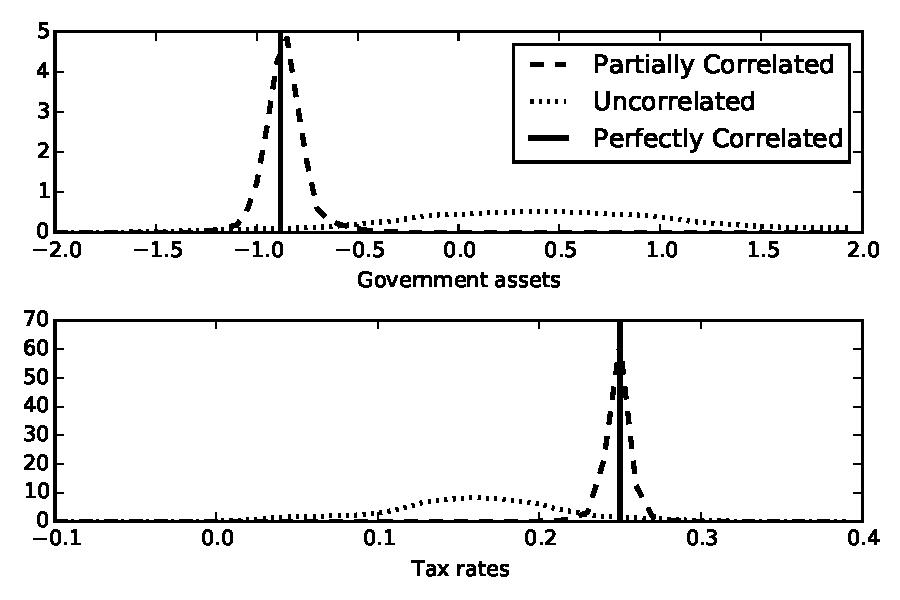
\includegraphics[width=7in]{plots/ErgodicQL.pdf}
 \caption{Ergodic distribution for debt and taxes in the representative agent quasilinear economy for three choices $P(s)$. \textbf{Anmol and David XXXXX: I recommend
 trimming the range so that only positive densities are mostly shown.}}
 \label{fig: ergodic distribution ql}
 \end{figure}



\subsection{Heterogeneous agent economy with quasilinear preferences\label{sec:hetquasilinear}}

We now  turn to a more still restricted special economy, but one that now features both  heterogeneous agents and  transfers. We add to
the setion \ref{Sec: rep agent} representative agent economy  a second agent who has zero productivity and require that  his consumption be nonnegative. 
Given the Ricardian equivalence result discussed in section \ref{sec:Ricardian101}, 
we maintain a normalization that assets of the unproductive agent are zero throughout this section.
\begin{assumption}
 $\theta_1>\theta_2=0$  and $c_{2,t}\geq 0.$
\end{assumption}
The assumption that $\theta_2=0$  allows us to characterize how  the Ramsey plan  depends on the Pareto weights.
The nonnegativity constraint on the unskilled agent 2's consumption  adds enough  curvature to the Ramsy problem to unleash main forces
that will also prevail in more general settings. In these more general settings, risk aversion and Inada restrictions 
unleash the same forces.
%We now state the theorem and then discuss its implications.



\begin{theorem}
\label{thm heterogeneous agents}
Let $(\omega,n) \in [0,1] \times [0,1]$ be a Pareto weight and mass assigned to the  productive type $1$ agent.  Assume that $n<\frac{\gamma}{1+\gamma}$.
The optimal tax rate, transfer, and government asset policies $\{\tau_t,T_t,B_t\}$ are characterized as follows:


\begin{enumerate}
 \item For $\omega\geq n \left(\frac{1+\gamma}{\gamma}\right)$ we have  $T_t=0$ and the optimal policy is same as in the representative agent economy studied in 
 Theorems \ref{thm: rep agent general theorem},and \ref{thm: rep agent linear policies}
 \item For $\omega< n \left(\frac{1+\gamma}{\gamma}\right)$, suppose that $\min_{s}\{P(s)\}>\beta$.
 
 There exist  a $\mathcal{B}(\omega)$  satisfying $\mathcal{B}'(\omega)>0$ and  $\lim_{\omega\to 0}\mathcal{B}(\omega)<0$ and a $\tau^*(\omega)$ such that 
 \begin{enumerate}
  \item $B\_>\mathcal{B(\omega)}$
\[T_t>0, \quad \tau_t=\tau^*(\omega), \textit{ and } B_t=B\_ \quad \forall t \geq 0 \] 
\item $B\_\leq \mathcal{B(\omega)}$, the policies depend on the structure of $P(s)$. 
\begin{enumerate}
 \item For $P(s)\not \in \mathcal{P}^*$
 
   \[ T_t>0 \text{ i.o.},\quad \lim_t\tau_t=\tau^*(\omega) \text{ and } \lim_tB_t=\mathcal{B}(\omega)\quad \textit{a.s}\]

 \item For $P(s)\in \mathcal{P}^*$, we have two cases depending on $B\_$
\begin{enumerate}
 \item For $B\_\leq B^*$ 
 \[T_t = 0, \quad \lim_t \tau_t=\tau^{**} (\omega), \textit{ and } \lim_tB_t=  B^*\quad a.s \]
\item For $\mathcal{B}(\omega)>B\_>B^*$
\small
\[\Pr\{\lim_t T_t = 0, \lim_t \tau_t=\tau^{**}(\omega),\lim_tB_t=  B^* \textrm{ or }  T_t>0 \text{ i.o.},\lim_t\tau_t=\tau^*(\omega), \lim_tB_t=\mathcal{B}(\omega) \}>0 \]
 \normalsize 
\end{enumerate}


 \end{enumerate}

 \end{enumerate}

 \end{enumerate}


\end{theorem}

In the theorem \ref{thm heterogeneous agents} two types economy, 
% using fluctuations in transfers to hedge aggregate shocks imposes utility costs on the zero skilled ($\theta_{2,t} =0$)
% type 2 agents. The Ramsey planner balances these costs against the efficiency costs associated with fluctuations in the tax rate on labor.  How the planner
% strikes this balance depends on the Pareto weight $\omega$ attached to the higher skilled type $1$ agent.  For sufficiently high $\omega$, the planner opts for productive
% efficiency
Ramsey planner bears costs of using  fluctuating transfers to hedge aggregate shocks.
The  environment is simple enough to allow us to pinpoint how these costs depend on the Pareto weights.
For a ``regressive'' planner who cares more about the productive type 1 agents, 
 using transfers is especially costly.   For a high $\omega$ Pareto planner, increasing transfers  entails subsidizing the unproductive type 2 agents
whose consumption he values little. A Ramsey planner who assigns  a Pareto weight $\omega$ to the productive type 1 agent above a 
threshold $\bar{\omega}=n\left(\frac{1+\gamma}{\gamma}\right)$ sets transfers to zero always.  This makes  the Ramsey  plan
in the theorem \ref{thm heterogeneous agents} two-type of agents economy be  identical to the plan for the representative agent economy
of theorem \ref{thm: rep agent general theorem}: when $\omega \geq \bar \omega$, the type type 1 agent
in effect becomes the representative agent of the theorem \ref{thm: rep agent general theorem} economy.   However, 
for a less regressive  $\omega<\bar{\omega}$ Ramsey planner, 
transfers remain a useful tool for subsidizing the unproductive agent. To finance these transfers, the Ramsey planner
chooses to  tax the labor income of the  productive agent and  need not accumulate a large buffer stock of assets. 
Thus, the  limiting stock of government  assets is lower and tax rates are larger  for sufficiently more redistributive Ramsey planners.


\section{More general economies}
\label{Sec: more general economies}
To facilitate analysis, the section \ref{sec:hetquasilinear} economy simplifies things along several dimensions: there is no
curvature in the utility from consumption, shocks lack  persistence  shocks,  and there are only two agents.
These simplifications make the return on debt be exogenous and equal to $\beta^{-1}P(s)$.
Adding curvature to utility from consumption  makes the returns on debt endogenous even for a standard risk-free bond having a payoff vector $P(s)=1$.
Adding curvature requires keeping track of relative marginal utilities of consumption in order to characterize how  the Ramsey planner makes the  tax rate, government debt, 
and transfers respond to shocks.
This confounds the effects of the planner's motives to redistribute and to use the level of government debt in conjunction  with fluctuations in the 
rate of interest  to hedge shocks to government expenditure and  productivity. 


In the next subsection, we first show that with curvature in the utility from consumption, there exists a level of government debt that allows the government
completely to hedge expenditure shocks only if those shocks are binary and IID.
We provide an associated example  with CES preferences in which  as time passes the Ramsey plan approaches  constant ratios of  consumption and a constant
labor tax rate. We also show that how the comovement of the  interest rate with exogenous shocks governs the governments' incentives
to accumulate assets, an outcome reminiscent of  outcomes in the
section \ref{sec:hetquasilinear}  economy with quasilinear preferences.



\subsection{Eventual complete hedging with binary shocks}

For a given state $\left(
\bm{x},\bm{\rho },s\_\right) $, let  $\Psi \left( s;\bm{x},%
\bm{\rho },s\_\right) =\left( x^{\prime }\left( s\right) ,\rho ^{\prime
}\left( s\right) \right) $  solve (\ref{eq:BM2})so that $\Psi \left( s;\bm{x},\bm{\rho },s\_\right) $ is an optimal  law of motion for the state variables
under a Ramsey plan at $t \geq 1$. 
\begin{definition}
 A steady state % $\left( \bm{x}^{SS},\bm{\rho} ^{SS}\right) $  
 satisfies $\left(\bm{ x}^{SS},\bm{\rho}
^{SS}\right) =\Psi \left( s;\bm{x}^{SS},\bm{\rho} ^{SS},s_{-}\right) $ for all $%
\,s,s\_.$
\end{definition}
In a steady state, the ratios  of marginal utilities  $\rho_i =U_{c}^{i}(s)/U_{c}^{1}(s)$ are constant  and so do
not depend on   $s$.
%the ratios of marginal utilities
%of  all agents are constant. 
This means that in a steady state, the continuation allocation depends only on  $s_{t}$ and not on the  history $s^{t-1}$.% These outcomes are reminiscent though not quite identical to those in a complete market economy (see Werning
%2007).\footnote{\textcolor{blue}{David, I have changed it a bit, do you think it reflects our understanding better. The earlier one sounded too cautionary}
%The steady state allocation is optimal for a \emph{modified} complete market problem where the Planner has to additionally adhere to a specific ratio of pairwise consumption (or ``market weights'' as in Werning(2007). However we note that typically, there does not exist an initial distribution of  assets  and list of Pareto weights for which the optimal allocation with complete markets will \emph{coincide} with the aforementioned stationary allocation with incomplete markets.}



A competitive equilibrium  allocation $\{c_i(s),l_i(s)\}_{i}$ associated with a choice for $\{\tau(s), \bm{\rho}(s)\}$ is determined by
equations (\ref{eq:BM2_Wages_cons}), (\ref{eq:BM2_Res_cons}) and (\ref{eq:BM2_rhoprime}).  Denote $U(\tau,\bm{\rho},s)$ as
the value of that competitive equilibrium allocation to a planner with Pareto weights $\{\omega_i\}_i$:
\[U(\tau,\bm{\rho},s)=\sum_{i}\omega_i U^i(s).\]
\textbf{Anmol XXXXX: do you not want $\omega$ as an argument of $U$?}
As before define $Z_i(\tau,\rho,s)$ as
\[Z_i(\tau,\bm \rho,s)=U^i_c(s)c_i(s)+U^i_l(s)l_i(s)-\rho_i(s)\left[U^1_c(s)c_1(s)+U^1_l(s)l_1(s)\right].\]
% Note that $\sum_{i=2}^{N}Z_i(\tau,\bm  \rho,s)$ is the marginal utility adjusted  primary deficit using the implied allocation.
%
%
%
% %Next we define $Z(\tau,\rho,s)$ as the marginal utility adjusted primary deficit using the implied allocation.
% \[Z(\tau, \bm \rho,s)=c_1^{-\sigma}(s)\left\{NT(s)+g-\tau(s)\sum_{i=1}^{N}\left[\theta_il_i(s)\right]\right\}\]
%
%
In the IID case,  the Ramsey optimal policy  solves the following Bellman equation in $\bm{x}(s^{t-1})=\bm{x},\bm{\rho}(s^{t-1})=\bm{\rho}$
%
 \begin{equation}
 \label{eq:ss-obj}
 	V(\bm x,\bm \rho) = \max_{\tau(s),\bm \rho'(s),\bm x'(s)}\sum_s \pi(s)\left[ U(\tau(s),\bm \rho'(s),s) + \beta(s) V(\bm x'(s),\bm \rho'(s))\right]
 \end{equation}
where the maximization is subject to the constraints
subject to the constraints
 \begin{equation}
 \label{eq:ss-imp}
 	Z_i(\tau(s),\bm \rho'(s),s) + x'_i(s) = \frac{x_i \beta^{-1}P(s) U^i_c(\tau(s),\bm \rho'(s),s)}{\mathbb{E} U^i_c(\tau,\rho)}\text{   for all  $s,i \geq 2$,}\\
 \end{equation}
\begin{equation}
\label{eq:bondcondtion}
 	\sum_s \pi(s)P(s)U^1_c(\tau(s),\bm \rho'(s),s)(\rho_i'(s)-\rho_i) = 0 \text{  for $i \geq 2.$}
\end{equation}
 Constraint (\ref{eq:bondcondtion}), which rearranges constraint (\ref{eq:BM2_Bonds_cons}),  implies that $\rho(s)$ is a risk-adjusted martingale.
 
 Our  next job is to study conditions that allow the first-order necessary conditions to be   consistent with the existence of stationary policies 
 for some ($\bm x, \bm \rho$).\footnote{Appendix \ref{apndx: numerical methods} discuses  second-order conditions that ensure these policies are optimal.}
 \textbf{Anmol XXXXX: has a notion of ``stationary policies'' been defined anywhere?  Either it should be or the preceding sentence should be made more precise.}
 \begin{lemma}\label{lemma-simplified-foc}
With the utility is strictly concave in consumption,  $\|S\|=2$ is necessary for a steady state to exist. \textbf{Anmol: is this precisely what you want to say -- necessity
versus sufficiency?}
 \end{lemma}
 \begin{proof}
   Let $\pi(s)\mu_i(s)$ and $\lambda_i$ be Lagrange multipliers on constraints (\ref{eq:ss-imp}) and (\ref{eq:bondcondtion}).  
   Imposing the restrictions $x'_i(s) = x_i$ and $\rho'_i(s) = \rho_i$, at a  steady state  $\{\mu_i,\lambda_i,x_i,\rho_i\}^{N}_{i=2}$ and $\{\tau(s)\}_s$
are determined by  the following equations:
\begin{subequations}
\label{sys-steadystate}
\begin{equation}
\label{eq:ss.imp.simplified}
  	Z_i(\tau(s),\bm \rho,s) + x_i = \frac{\beta^{-1}P(s)x_i U^i_c(\tau(s),\bm \rho,s)}{\mathbb{E} U^i_c(\tau,\rho)}\text{   for all  $s,i \geq 2$,}\\
\end{equation}
 \begin{equation}
	U_{\tau}(\tau(s),\bm \rho,s)-\sum_i\mu_i Z_{i,\tau}(\tau(s),\bm \rho,s)  =0 \text{  for all $s$,} \label{eq:foc.tau.simplified}\\
   \end{equation}
\begin{equation}
	U_{\rho_i}(\tau(s),\bm \rho,s) -\sum_j\mu_jZ_{j,\rho_i}(\tau(s),\bm \rho,s)+ \lambda_iP(s)U^1_c(\tau(s),\bm \rho,s)-\lambda_i\beta\mathbb{E}P(s)U^1_c(\tau(s),\bm \rho(s),s) =0. \text{   for all $s,i \geq 2$ }\label{eq:foc.R.simplified}
 \end{equation}
\end{subequations}
Since the shock $s$ takes only two values, \eqref{sys-steadystate} is a square system in $4(N-1)+2$ unknowns $\{\mu^{SS}_i,\lambda^{SS}_i,x^{SS}_i,\rho^{SS}_i\}^{N}_{i=2}$ and $\{\tau^{SS}(s)\}_{s}$. \end{proof}

At a steady state, outcomes resemble those in  the complete market economy of \citet{Wer07a}. 
The tax rate  and transfers both depend only on the current realization of shock $s_t$. 
Furthermore,  arguments of \citeauthor{Wer07a} can be adapted  to show that the tax rate is
constant when preferences have the CES form $c^{1-\sigma}/(1-\sigma) - l^{1+\gamma}/(1-\gamma) $,  and also that fluctuations in the tax rate
are very small when preferences take forms consistent with the existence of  balanced growth. We return to this point  after we discuss convergence to a steady state.

To 
verify existence of a steady state for a particular set of  parameter values requires checking that there exists a solution of system (\ref{sys-steadystate}). 
Since  (\ref{sys-steadystate}) is a non-linear system, existence can   be verified only numerically in general. However, sometimes more can be established.
Thus, we now provide a simple example with risk averse agents in which the existence of a root of (\ref{sys-steadystate}) can be established analytically. The
analytical characterization of the steady state in this special case will help us  develop some comparative statics and some connections between the quasilinear economy
of section \ref{sec:hetquasilinear} and  the more general economies to be analyzed quantitatively  in section \ref{sec: numerical results}.


\subsubsection{A two-agent example}\label{sec: 2 agent example}


Consider an economy consisting of  two types of households with $%
\theta _{1,t}>\theta _{2,t}=0$ and common one-period utilities  $\ln c-\frac{1}{2}%
l^{2}.$ The shock $s$  takes  two values$ \left\{
s_{L},s_{H}\right\} $ with probabilities $\Pr \left( s|s\_\right) $ that are
independent of $s_{-}.$ We assume that $g\left( s\right) =g$ for all $s,$
and $\theta _{1}\left( s_{H}\right) >\theta _{1}\left( s_{L}\right) .$ We allow the discount factor $\beta(s)$ to depend on  $s.$

\smallskip

\begin{theorem}
\label{thm long run forces}\smallskip Suppose that $g<\theta (s)$ for all $%
s.$ Let $R(s)$ be the gross interest rate and $x=U^2_c(s)\left[b_2(s)-b_1(s)\right]$

\begin{enumerate}
\item \textbf{Countercyclical interest rate.} If $P \left( s_{H}\right) =P\left( s_{L}\right)$, then
there exists a steady state $\left( x^{SS},\rho ^{SS}\right) $ such that $%
x^{SS}>0,\ R^{SS}\left( s_{H}\right) <R^{SS}\left( s_{L}\right) .$
\item \textbf{Procyclical interest rate.} There exists a pair  $\left\{ P \left( s_{H}\right) ,P\left( s_{L}\right)
\right\} $ such that there exists a steady state with $x^{SS}<0$ and  $R^{SS}\left( s_{H}\right) >R^{SS}\left( s_{L}\right) .$
\end{enumerate}
In both cases, the tax rate $\tau(s)=\tau^{SS}$ is independent of $s$.
\end{theorem}


By setting the assets of the unproductive agent to zero, which theorem \ref{theorem: main} tells us amounts only to  a normalization,
we can interpret $x$ as the marginal-utility-adjusted assets of the government. \textbf{Anmol XXXXX: please check the previous important sentence which I edited 
and may have degraded.}
Besides establishing existence of a steady state, theorem \ref{thm long run forces} 
emphasizes the cyclical properties of the real interest rate as a determinant of the the sign of government assets under a Ramsey plan.

Theorem \ref{thm long run forces}  highlights  two main forces that determine the dynamics of the  tax rate
and government assets: fluctuations in inequality and fluctuations in the interest rate. Keeping  the interest rate fixed for the moment, the government can in principle adjust two
instruments in response  to an adverse  shock (i.e., a fall in $\theta_1$): it can either increase the  tax rate $%
\tau $ or it can decrease transfers $T.$ Both  responses are distorting,
but for different reasons. Increasing the tax rate increases distortions because the deadweight loss is convex in the tax rate,
 as in \cite{Barro1979}. The Ramsey planner copes with this distortion  in the present economy in the same way that it does in  representative agent economies.
 But in a  heterogeneous agent economy like ours,  adjusting transfers $T$ is
also costly. When agents' asset holdings are identical, \textbf{Anmol XXXXXX: but they aren't identical in this setting are they?}
a decrease in transfers  disproportionately
affects a low-skilled agent, so his marginal utility
falls by more than does the marginal utility of a high-skilled agent. Consequently, a
decrease in transfers increases inequality, giving rise to a cost  not present in  representative agent economies.

The government can reduce the costs of  inequality distortions by choosing
tax rate policies that make the net asset positions of  the high-skilled agent
decrease over time. That makes the two agents'
after-tax and after-interest income  become closer, allowing decreases in transfers to have smaller effects on inequality in
marginal utilities. If the net asset position of a high-skilled agent is
sufficiently low, then a change in transfers has no effect on inequality and
all  distortions from fluctuations in transfers are eliminated.\footnote{This convergence outcome has
 a similar flavor to "back-loading"\ results  of
 \cite{Ray2002} and \cite{Albanesi2012} that reflect the  optimality of structuring policies intertemporally eventually to disarm  distortions.}




%
% If consumption is ordered i.e it is higher in booms than in recessions, interest rates are countercyclical. The government will hold positive assets as long as the steady state marginal utility adjusted primary deficit$Z(\tau,\rho,s)$ is countercyclical too.

% It is possible to show numerically\footnote{Appendix \ref{apndx: numerical methods} describes a numerical test for existence and local stability cast in terms of  primitives.} that the steady state described in part
% 2 of  proposition \ref{thm long run forces} is stable, so the  economy converges to it. This convergence outcome has
% a similar flavor to "back-loading"\ results  of
% \cite{Ray2002} and \cite{Albanesi2012} that reflect the  optimality of structuring policies intertemporally eventually to disarm  distortions.

% Theorem \ref{theorem: main} provides  a useful way to compare our results with
%  representative agent economies. By that theorem, we can normalize $%
% b_{2,t}=0 $ for all $t$, in which case the negative of net assets of high-skilled agents can be
% interpreted as assets of the government. Because $x^{SS}>0,$
% the government  accumulates assets over time$,$ as in  AMSS.

% the government  accumulates assets over time$,$ as in  AMSS.

 Turning now to the second force, the  interest rate generally fluctuates
 with  shocks.  Parts 1 and 2 of  theorem \ref{thm long run forces} isolates forces that  drive those  fluctuations. 
 Consider again the example of a
 decrease in the productivity of high-skilled agents. If the  tax rate  $\tau $ is left unchanged,
 %the government faces a shortfall of revenues. Since
 since $g$ is constant, the
 government requires  extra revenues. But  suppose that
 the interest rate increases whenever $\theta_1 $ decreases, as happens, for
 example, with a risk free bond. If the government holds positive assets, its earnings from those assets increase. 
 So holding assets allows higher interest income  to offset some of the government's revenue losses from taxes on labor.
 The situation reverses if the interest rate falls at
 times of increased need for government revenues, as in
  part 2 of  theorem \ref{thm long run forces}, so the steady state allocation features the government's owning debt. 
  
  These outcomes have  counterparts in  the representative agent quasilinear economy studied in section \ref{Sec: quasilinear}.
  There, exploiting linearity allowed us to provide a sharper characterization of how the covariance of the interest rate
  and  exogenous shocks affected the sign (and level) of debt through expression \eqref{ss-debt}. 
  In parts 1 and 2 of theorem \ref{thm long run forces}, with binary shocks,  altering the gap $P(s_H)-P(s_L)$ allows 
  us to obtain a corresponding variation in interest rates. The reasoning and  underling forces are the same.
  
\subsection{Stability}\label{sec:stability}
We extend the Theorem \ref{thm: rep agent linear policies}  approximation methods  to more general economies with strictly concave utility functions.
 Unlike  the quasilinear case where we could obtain an analytical characterization, here 
 we present a numerical  convergence criterion and use it to  show local stability of a steady state for a wide range of parameters. 

As before, let $\pi(s)\mu_i(s)$ and $\lambda_i$ be Lagrange multipliers on constraints (\ref{eq:ss-imp}) and (\ref{eq:bondcondtion}). 
In Appendix \ref{apndx: numerical methods} we show that the history-dependent optimal policies 
(they are sequences of functions of $s^t$) can be represented  recursively in terms of $\{\bm \mu(s^{t-1}),\bm \rho(s^{t-1})\}$ and $s_t$.
A recursive representation of an optimal policy can be linearized around  steady state values of the state 
variables  $(\bm{\mu},\bm{\rho})$.\footnote{One could  in principle look for a solution in state variables $\left(\bm{x}(s^{t-1}),\bm{\rho}(s^{t-1})\right)$.
For $I=2$ with $\{\theta_i(s)\}$ different across agents, this would give identical policies and a map that is (locally) invertible between $\bm{x}$ and $\bm{\mu}$ for
a given $\bm{\rho}$. However in other cases, it turns out there are unique linear policies in $(\
bm{\mu},\bm{\rho}
)$ and not necessarily in  $(\bm{x},\bm{\rho})$. This comes from the fact that the set of feasible $(\bm{x},\bm{\rho})$ are restricted at time 0 and may not contain an open set around the steady state values. When we linearize using $(\bm{\mu},\bm{\rho})$ as state variables, the optimal policies for $\bm{x}(s^t),\bm{\rho}(s^t)$ converge to their  steady state levels for all perturbations in $(\bm{\mu},\bm{\rho})$.}
Let $\hat{\Psi}_{t}= \left[\bmat \bm{\mu}_{t} - \bm{\mu}^{SS}\\ \bm \rho_t - \bm \rho^{SS}\emat\right]$ be  deviations from a steady state.
Construct a  linear approximation  
\begin{equation}
 \hat{\Psi}_{t+1}=B(s_{t+1})\hat{\Psi}_t. \label{eq.linear.lom}
\end{equation}
This linearized system has coefficients $B(s)$  that are functions of the shock. The next theorem describes a simple numerical test that allows us to determine whether  this linear system converges to zero in probability.

\begin{theorem}\label{thm: localstability}
If the (real parts) of the eigenvalues of $\mathbb{E}B(s)$ are less than 1,  system (\ref{eq.linear.lom}) converges to zero  in mean.
Further for large $t$, the conditional variance of $\hat{\Psi}$, denoted by $\Sigma_{\Psi,t}$, is governed by
\[\text{vec}(\Sigma_{\Psi,t})=\hat{B} \text{vec}(\Sigma_{\Psi,t-1}),\]	
where $\hat{B}$ is a square matrix of dimension $(2I-2)^2$. In addition,  if the (real parts) of the eigenvalues of $\hat{B}$ are less than 1, system \eqref{eq.linear.lom}
converges in probability.
\end{theorem}

The dominant  eigenvalue is informative not only about whether the system is locally stable but also about  how quickly the steady state is reached. 
The half-life of convergence to the steady state is  $\frac{\log(0.5)}{\|\iota\|}$, where $\|\iota\|$ is the absolute value of the dominant eigenvalue.
Thus, the closer the dominant eigenvalue is to one, the slower is the speed of convergence.

We have applied  Theorem \ref{thm: localstability} to verify local stability for a wide range of examples. 
Since the parameter space is high dimensional, we relegate the comparative statics to Appendix \ref{apndx: stability}.
The typical finding there  is that the steady state is stable but that convergence is slow.
The rates of convergence are increasing in the covariance of interest rates and the government's need for revenue. \textbf{Anmol XXXXX: do we want to tighten up
the concept `govt need for revenue' -- which has not been defined formally but is recurrently used. Is it $g_t + T_t$ or ????}












\section{Numerical example}
\label{sec: numerical results}
In sections \ref{Sec: quasilinear} and \ref{Sec: more general economies},
we studied steady states as a way of summarizing the asymptotic  behavior of Ramsey allocations and the forces that shape  the asymptotic level of government and private assets. 
In this section, we use a calibrated version of the economy  a) to revisit the magnitude of these forces; and  b) to study optimal policy responses 
at business cycle frequencies when the economy is possibly far away from a (stochastic) steady state. 
We choose shocks and initial conditions to match stylized facts from the  recent
recession in US. The numerical calculations use methods adapted from Evans (2014)
\textbf{Anmol and David -- let's add Evans (2014) properly to the *.bib file please.} 
and described  in the Appendix \ref{}. The next section describes how we set  parameters and initial conditions.
 


\subsection{Calibration}

We assume  five types of agents\footnote{We report the results for $N=5$ to capture sufficient heterogeneity in wealth and earnings. 
Our methods let  solve for arbitrary number of agents. We have verified that the main qualitative and quantitative insights are unchanged when  we
have more than five types.} of equal measures with preferences $u(c,l)=\frac{c^{1-\sigma}}{1-\sigma}-\frac{l^{1+\gamma}}{1+\gamma}$. 
These agents stand in for  the $90\textsuperscript{th},75\textsuperscript{th},50\textsuperscript{th},25\textsuperscript{th},  \text{and } 10\textsuperscript{th}$ quantiles
of the  US wage distribution. 

Let $\mathcal{Q}(i)$ be the quantile of agent $i$. We assume i.i.d aggregate shocks $\epsilon_t$ that affect both the labor productivities of all agents $\{\theta_{i,t}\}^{N}_{i=1}$ and the  payoff $p_t$ of the single asset:
\begin{subequations}
\begin{equation*}
 \log \theta_{i,t}=\log\bar{\theta_i}+ \epsilon_t[1+(.9-\mathcal{Q}(i))m]
\end{equation*}
 \begin{equation*}
p_t=1+\chi \epsilon_t 
 \end{equation*}

\end{subequations}
Following \cite{Autor2008},we set average productivities $\{\bar{\theta_i}\}^{N}_{i=1}$  to match
quantiles of  average weekly earnings of full time wage and salary earners from the Current Population Survey (CPS). 

The parameter $m$ allows us to generate recessions associated with different  falls in income for different types of agents.
We calibrate $m$ to match  facts reported by \citet{Fatih2014}.
Figure \ref{fig:fatih_picture} (adapted from \citeauthor{Fatih2014}) reports that in the latest US recession the fall in income for  agents in the first decile of earnings was about  three times 
that experienced by the 90th percentile. Furthermore, between the 10th and the 90th  percentiles, the change in the percentage drop in earnings was almost linear. 
From these facts we infer a slope  $m=\frac{1.5}{0.8}$. 

 {
  \begin{figure}
  \label{fig:fatih_picture}
    \centering
    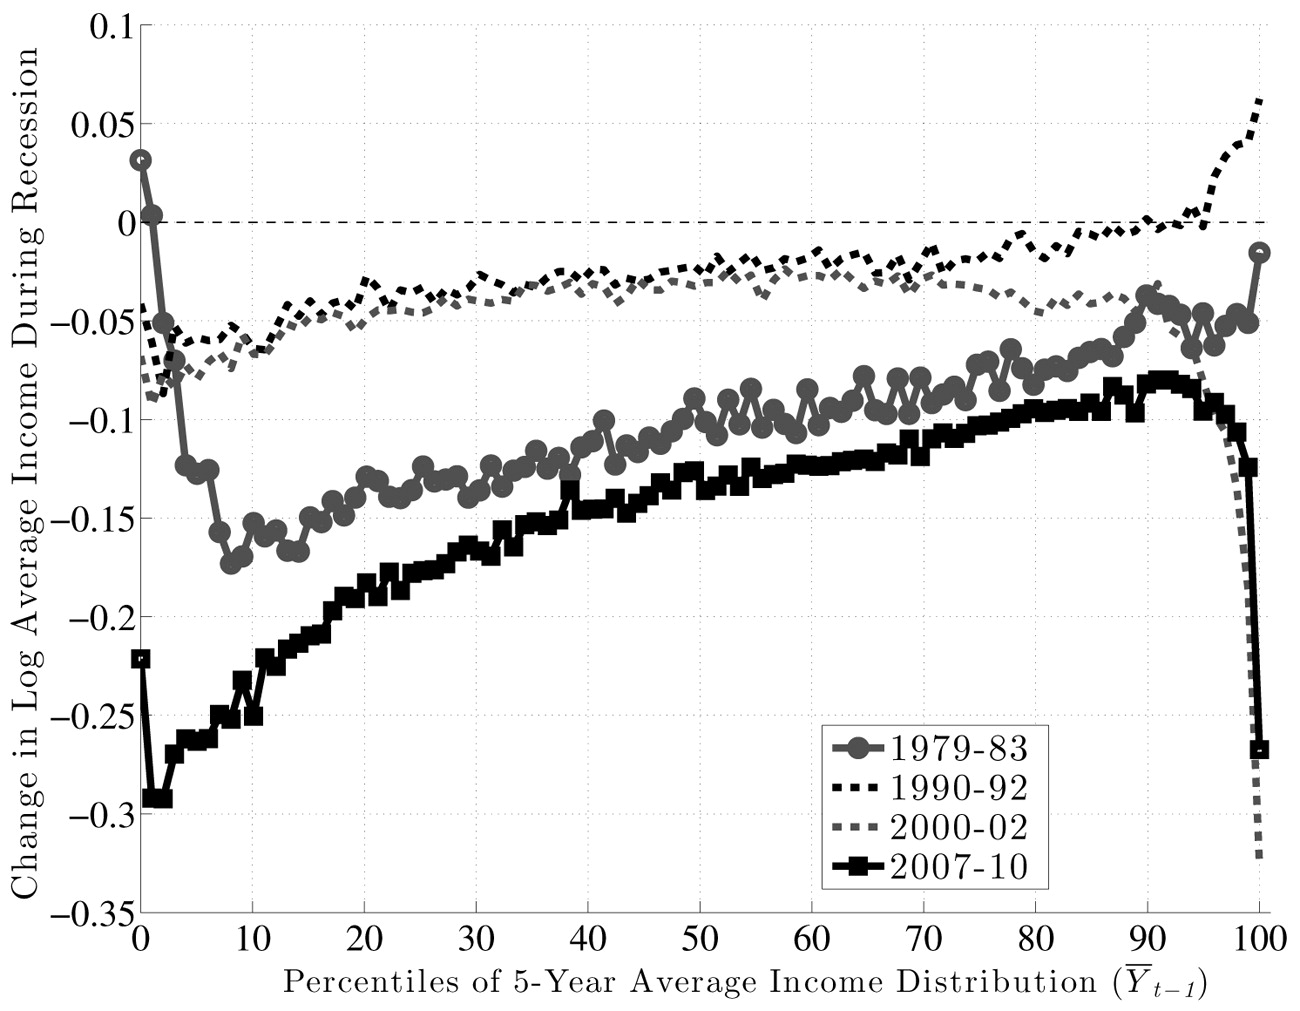
\includegraphics[width = 0.5\textwidth]{fg13.jpeg}
    \caption{ Change in log average earnings during recessions, prime-age males from \cite{Fatih2014}}
  \end{figure}

}

The parameter $\chi$ captures the ex-post comovement in returns on government assets  and aggregate shocks. 
Our model is silent about the source of these comovements. In the data,  they could 
compe from variations in real payoffs due inflation, interest rate risk for longer maturity bonds,  or defaults.
For the purpose of our numerical exercise, we use US data on inflation and interest rates of longer maturities bonds to calibrate $\chi$. 
We calibrate the comovement in the following way. 
Let $q^{(n)}_t$ be the log price of a nominal bond of maturity $n$. We can define  real holding period returns $r^{(n)}_{t,t+1}$ as
 
 \[r^{(n)}_{t,t+1}= q^{(n-1)}_{t+1}-q_t^{(n)}-\pi_{t+1}\]
 With the transfromation $y^{(n)}_t: -\frac{1}{n} q^{(n)}_t$ we can express $r^{(n)}_{t,t+1}$ as follows:
 \[r^{(n)}_{t,t+1}=\underbrace{y^{(n)}_t}_{\text{Ex-ante part}} - (n-1)\left[\underbrace{\left(y^{(n)}_{t+1}-y^{(n)}_{t}\right)}_{\text{Interest rate risk given $n$}}+\underbrace{\left(y^{(n-1)}_{t+1}-y^{(n)}_{t+1}\right)}_{\text{Term structure risk}}\right]-\underbrace{\pi_{t+1}}_{\text{Inflation risk}}\]

 In our model, the holding period returns are given by $\log\left[\frac{p_{t+1}}{q_{t}}\right]$ and $q_t=\frac{\beta \mathbb{E}_tu_{c,t+1}P_{t+1}}{u_{c,t}}$. Note that $p_{t+1}$ allows us to captures ex-post fluctuations in returns to the government's debt  portfolio coming from maturity and inflation. 
 
Table \ref{tab:corr} summarizes the comovement between labor productivity $\{\epsilon_t\}$ and bond prices $\{q^{n}_t\}$ for different maturities inferred from  quarterly US data for the period 1952 to 2003.
 \textbf{Anmol XXXXXX: a latex problem -- the automatic numbering of the table seems mixed up. See table and above sentence.}
The table's first line reports the correlation between the ex post returns and labor productivities. 
In our baseline calibration, $\epsilon_{t}$ is i.i.d over time. Hence the parameter $\chi=\frac{\sigma_{r}}{\sigma_{\epsilon}} Corr(r,\epsilon)$.
By averaging over different maturities we infer a value of $\chi=-0.06$. \footnote{The  second line of table \ref{tab:corr} computes
 the correlation of labor productivity with the  ex-post component of returns. 
For the shortest maturity, 3 month real tbill returns $ Corr(\epsilon_{t+1},y^{1 qtr}_{t}-\pi_{t+1})=-0.11$. These results together give us a 
range for $\chi$ of zero to negative $-0.09$. The numerical results are not sensitive to values of $\chi$ is this range.} Thus,
payoffs are weakly countercyclical for US. Besides the results for the benchmark value of $\chi=-0.06$, 
the long simulations in  section \ref{sec:longrunsimul} include outcomes for a  range of $\chi$'s from $-1.0$ to $1.0$.

\begin{table}[htp]
\begin{tabular}{|l|l| l|l|l|}
\hline
Maturity (n) &2yr & 3yr & 4yr & 5yr\\
\hline
$Corr(\epsilon_{t+1},r^{(n)}_{t,t+1})$ & -0.11 &-0.093 &-0.083 &-0.072\\
$Corr(\epsilon_{t+1},r^{(n)}_{t,t+1}-ny^{(n)}_{t})$& 0.00 & -0.0463 &-0.080& -0.091\\
$Corr(\epsilon_{t+1},y^{(n)}_{t}-\pi_{t+1})$ &-0.097  &-0.086  &-0.080  &-0.073 \\ 
$\frac{\sigma({r^{n}_{t+1}})}{\sigma({\epsilon_{t+1}})}$  &0.820  &0.835  &0.843  &0.845\\ 
\hline 
\end{tabular}
\caption{}
\label{tab:corr}
\end{table}

 
 
 As for  parameters of  household preferences, we set $\sigma=1$, $\gamma=2$, which imply Frisch elasticity of labor supply of $0.5$.
 We set the time discount factor $\beta=0.98$, which implies  the annual interest rate in an economy without shocks would be $2\%$ per year. 
 
 We assume that the initial wealth is perfectly correlated with wages and calibrate the wealth distribution to get the relative quantiles as in \cite{Kuhn2014} and
 Quadrini and Rios-Rull [2014]. \textbf{Anmol XXXXX: let's add appropriate reference to the *.bib file please.}
 These papers document the quantiles of net worth for US households computed up to 2010 Survey of Consumer Finances. 
 
 For the Pareto weights and government expenditures, we use an optimal allocation in an economy without shocks to target a (pre-transfers, federal) expenditure output ratio of $12\%$,
 a tax rate of $23\%$, a ratio of transfers to gdp of $10\%$, and a government debt to gdp of $100\%$. 
 


\begin{table}[htp]
\begin{tabular}{|l|c|p{4cm}|}
\hline
Parameter & Value & Description   \\ \hline
$\{\bar{\theta}_i\} $ & \{4.9,3.24,2.1,1.4,1\} & Wages dispersion for \{90,75,50,25,10\} percentiles   \\
$\gamma$ & 2 & Average Frisch elasticity of labor supply of 0.5 \\
$\beta$ & 0.98  &Average (annual) risk free interest rate of 2\%   \\
$m$ &$\frac{1.5}{.8}$& Heterogeneity in wage growth over business cycles\\
$\chi$ & -0.06 &Covariance between holding period returns and labor productivity\% \\
$\sigma_e$ & 0.03 & vol of labor productivity\\
$g$ & .13 \%&Average pre-transfer expenditure- output ratio of 12 \% \\\hline
\end{tabular}
\caption{Benchmark calibration}
\label{tab:Parameters}
\end{table} 
 
 
 
\subsection{Long run outcomes}\label{sec:longrunsimul}
Figure \ref{fig:long_simulation} simulations of  2000 periods for the government debt to output ratio, the labor tax rate,  and the transfers to output ratio
for three values of $\chi \in \{-1.0,-0.06,1.0\}$ in red, black, and blue, respectively. The three simulations start from the  same initial conditions and 
all share the same sequence of underlying shocks. 

 {
  \begin{figure}
  \label{fig:long_simulation}
    \centering
    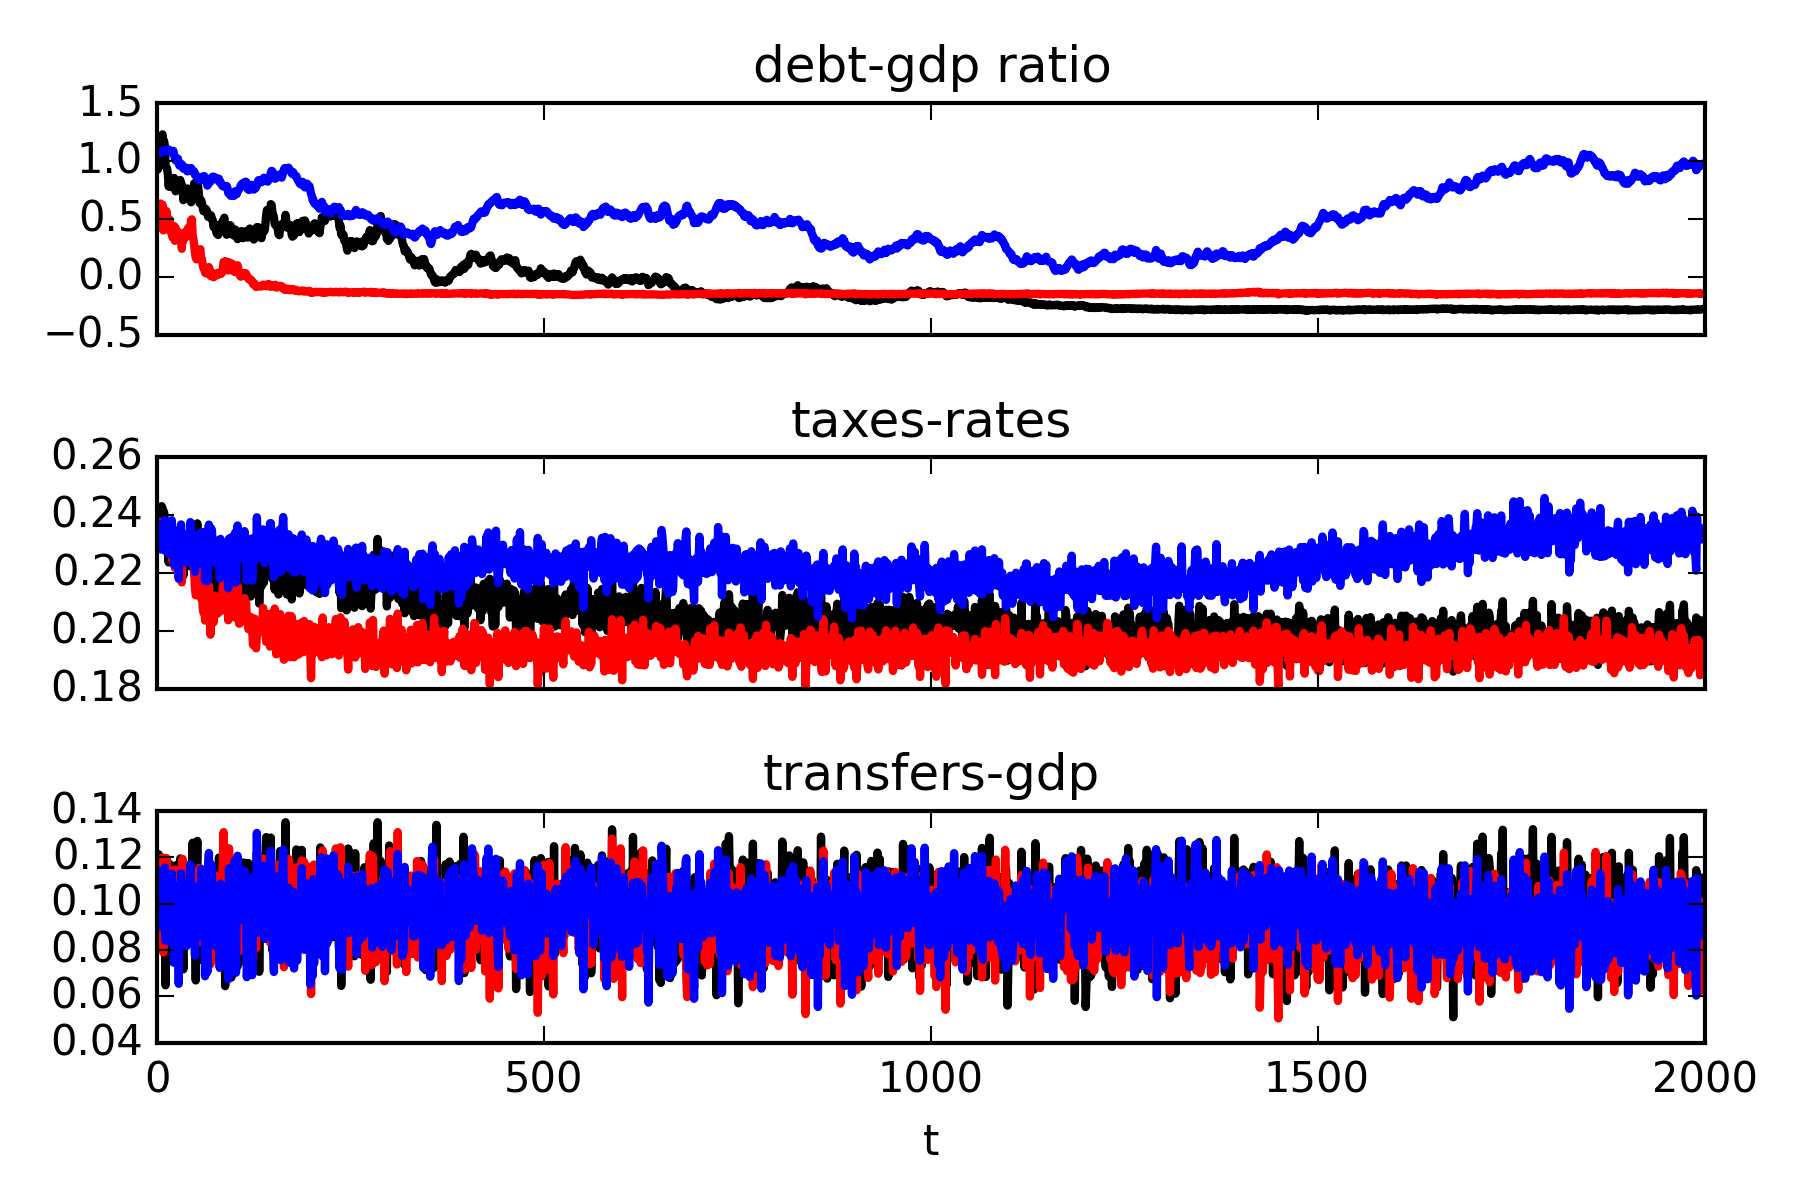
\includegraphics[width = 0.9\textwidth]{cesplots/long_simulation_debt.png}
    \caption{The red, black and blue lines plot simulations for a common sequence of shocks for values of $\chi=-1.0,-0.06,1.0$ respectively}
  \end{figure}

}

Two features emerge.   Different values $\chi$ give rise to different locations of the long-run marginal distribution of government assets and also to different  rates  of convergence 
to that long-run distribution.
A sufficiently positive $\chi$ generates lower payoffs in recessions relative to booms. In line with assertions of  theorems \ref{thm: rep agent general theorem} and  \ref{thm long run forces},
we see from the blue line  that  the government does not repay its initial debt during these 2000 periods. On the other
hand, under the benchmark $\chi$  (black line) or  when $\chi$ is negative (red line), the government accumulates assets. 

In order to get a clearer picture of the speed of convergence, we plot  paths of the conditional means for debt and the  tax rate in figure \ref{fig:speed_of_convergence}. 
To explain how we generated these plots, let $B(s_{t+1},\bm x_t, \bm \rho_t)$ be the Ramsey decision rules
that generate the assets $B$ of the government and let $\Psi \left( s_{t+1};\bm{x}_t,\bm{\rho }_t\right)$ be the law of motion for the state variables for the Ramsey plan.
For a given history, the conditional mean of government assets is:
\begin{subequations}
\begin{equation}
B^{cm}_{t+1}=\mathbb{E}B(s_{t+1},\bm x^{cm}_t,\bm \rho^{cm}_{t}) 
\end{equation}
 \begin{equation}
 \bm x^{cm}_t,\bm \rho^{cm}_{t}=\mathbb{E}\Psi (s_{t}, \bm x^{cm}_{t-1},\bm \rho^{cm}_{t-1}) 
 \end{equation}
\end{subequations}
Note how these conditional mean  paths smooth the high frequency movements in the dynamics of the state variables but retain the low frequency drifts.
 As before,  different lines correspond to  different values of $\chi$ between $-1.0$ and $1.0$ with the blue (red) lines representing positive (negative) values of $\chi$.
 Thicker  lines depict outcomes associated with larger values of $\chi$. The figure  shows that the speed of convergence is increasing and the magnitude of the limiting assets in decreasing 
 in the strength of correlation between productivities and payoffs. This pattern  confirms the approximation results characterized in theorem \ref{thm: rep agent linear policies}.

 {
  \begin{figure}
  \label{fig:speed_of_convergence}
    \centering
    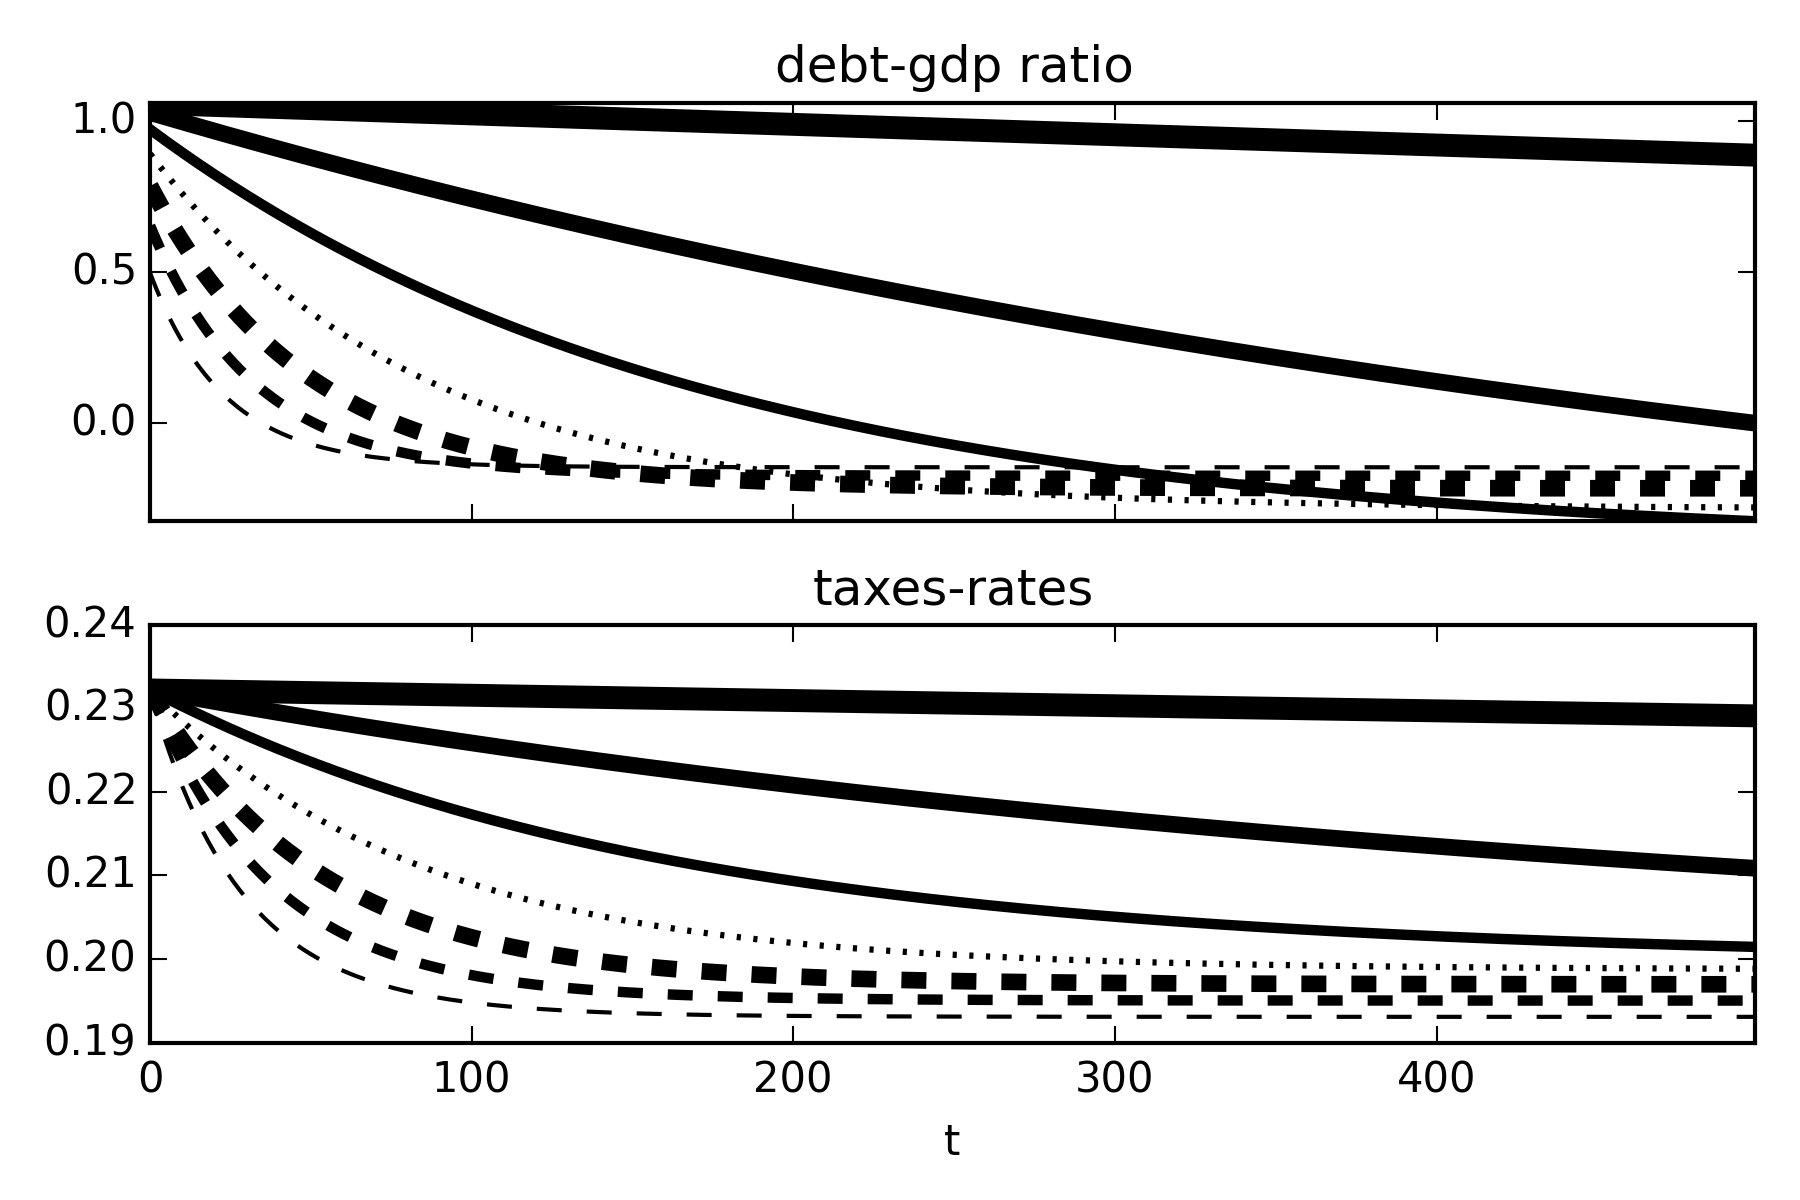
\includegraphics[width = .9\textwidth]{cesplots/speed_of_convergence.png}
    \caption{The plot shows conditional mean paths for different values of $\chi$. The red (blue) lines have $\chi<0$ ($\chi>0$). The thicker lines represent larger values.}
  \end{figure}

}


To verify the wide support of the ergodic distributions,
we take the initial conditions at the end of the long simulation and subject the economy to a sequence of 100 periods of $\epsilon_t$ shocks that  are 2 standard deviations below the mean.  In figure \ref{fig: wide support of taxes} we see that given a sufficiently long sequence of negative productivity  shocks the economy will eventually deviate significantly from its ergodic mean.


{
  \begin{figure}
  \label{fig: wide support of taxes}
    \centering
    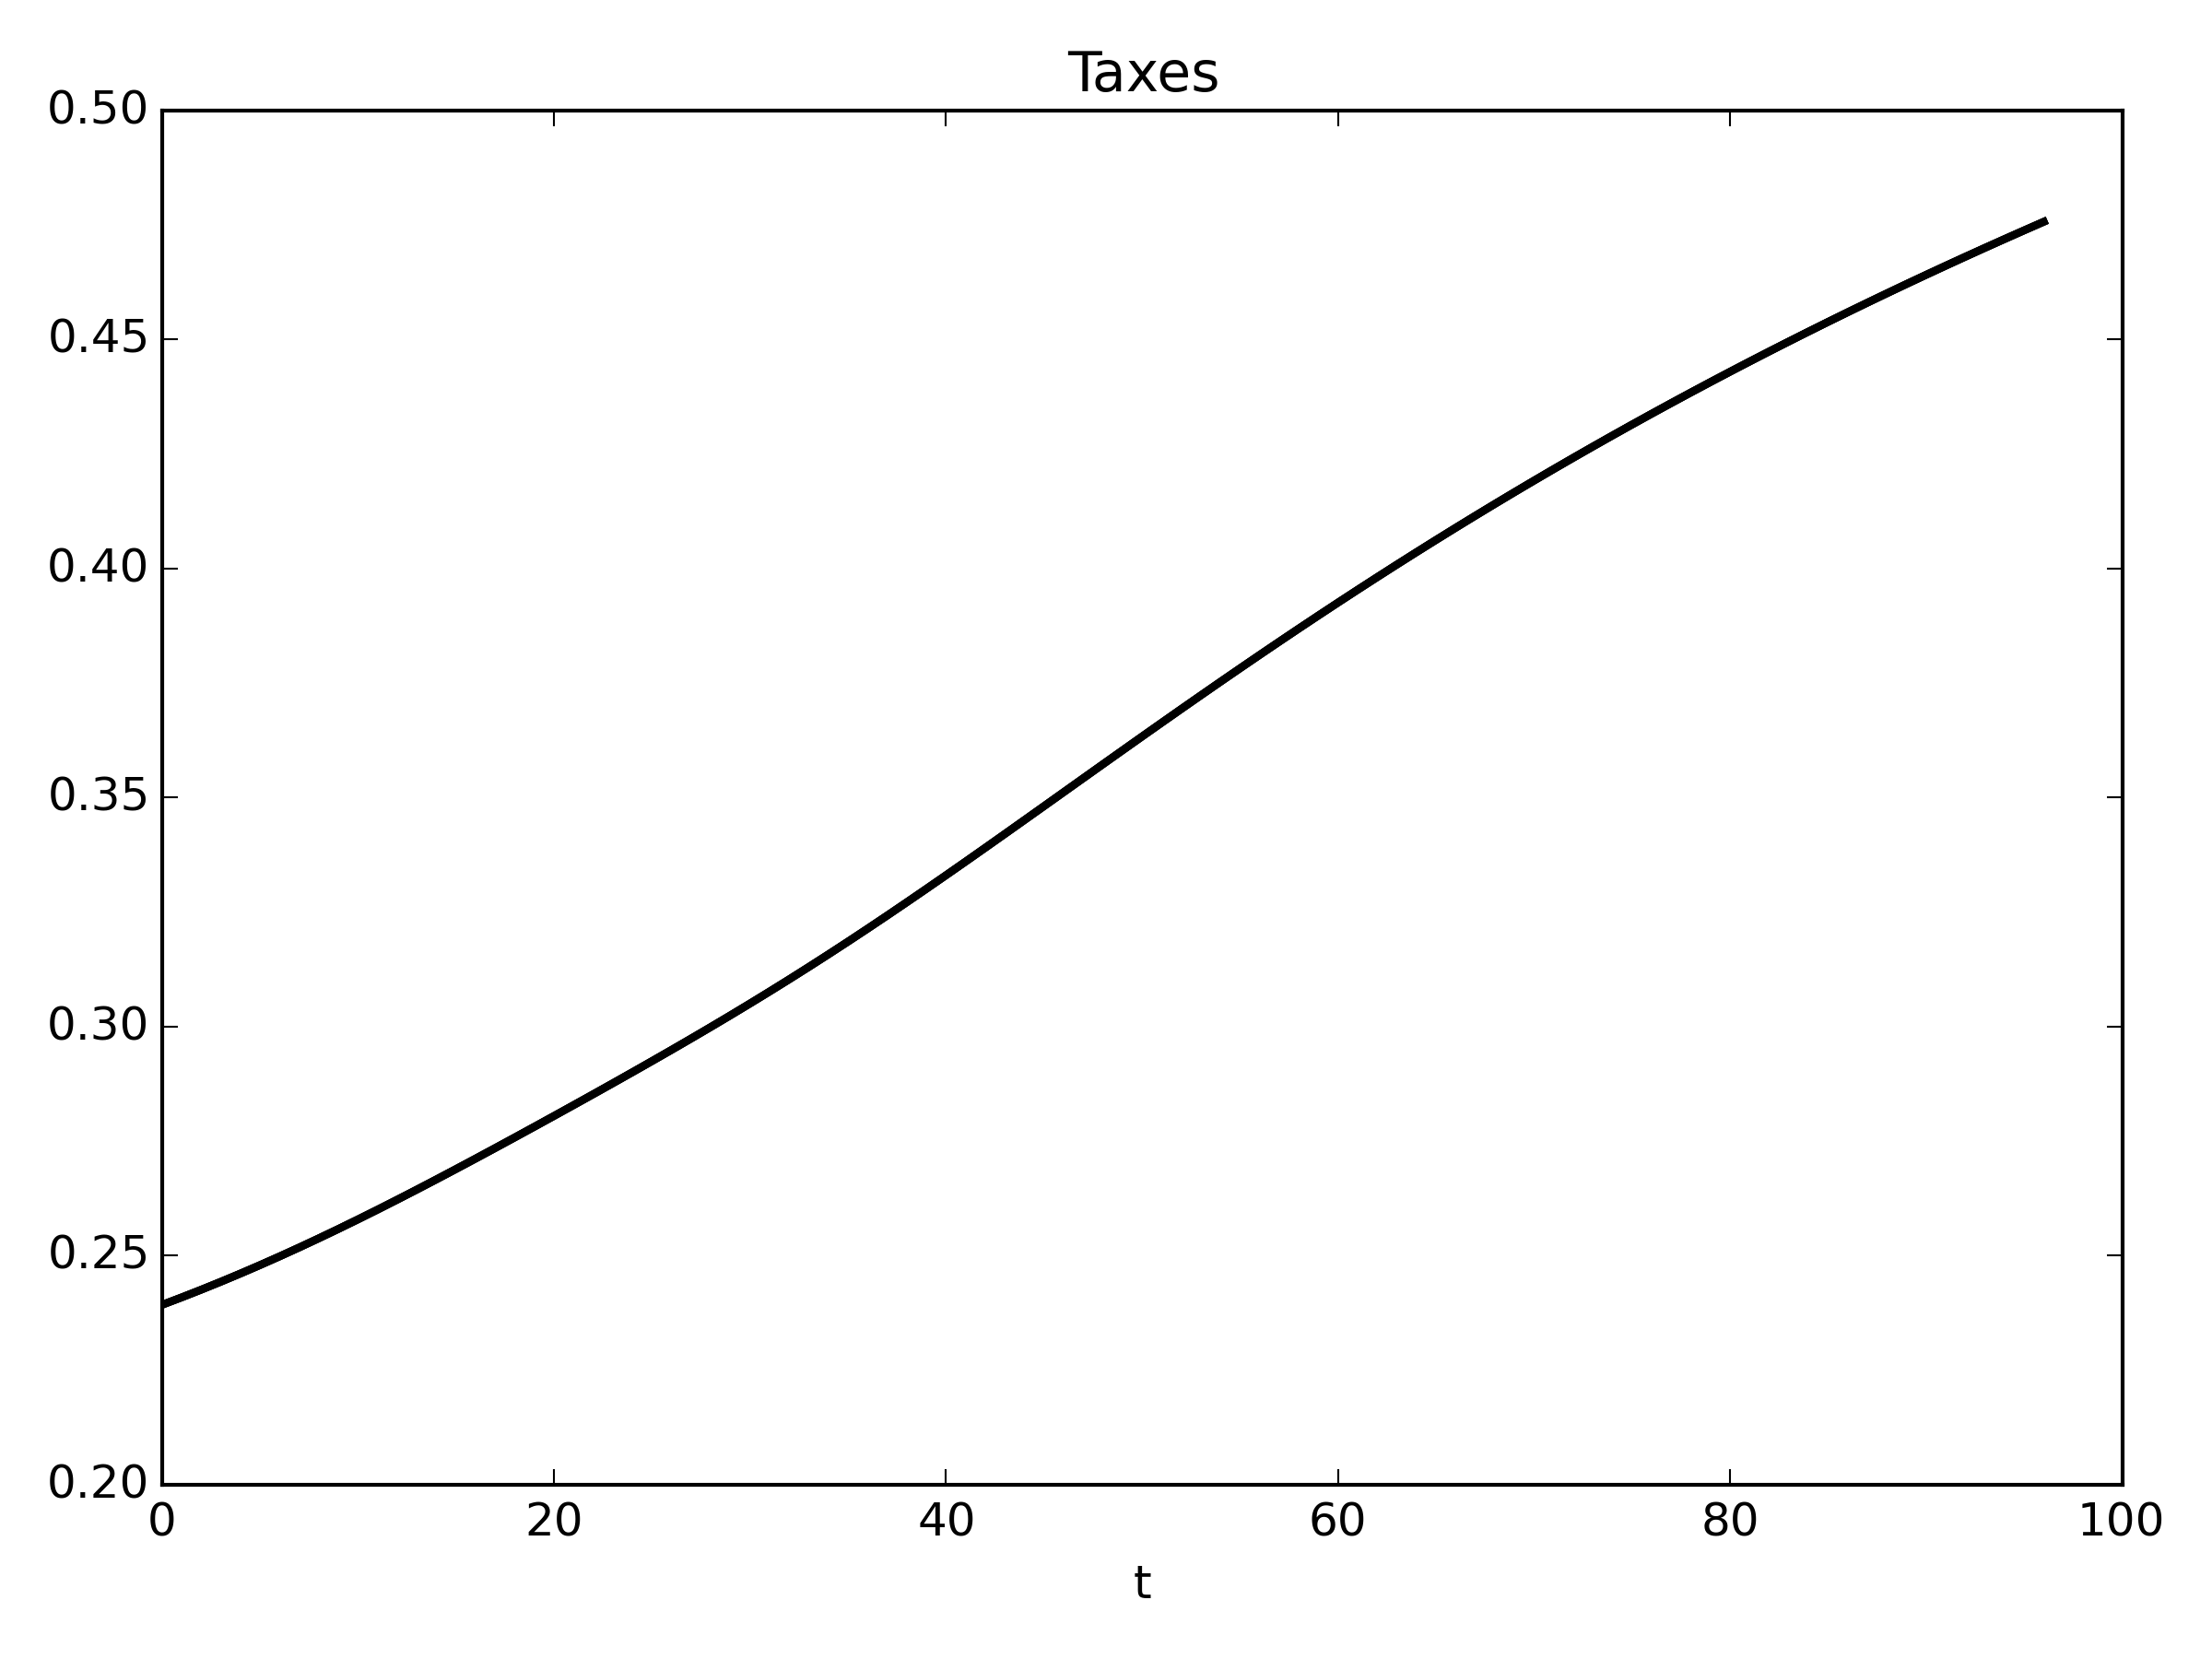
\includegraphics[width = 0.8\textwidth]{cesplots/taxes_only_bad_shocks.png}
    \caption{Taxes for a sequence of -1 s.d shocks to aggregate productivity of length 100}
  \end{figure}

} 

A further inference from the analysis of earlier sections was that government assets $B$  in the steady state are decreasing in the redistributive motive of the government. 
We check this numerically here  by changing  Pareto weights.  In the baseline case analyzed in this section so far, there are equal Pareto weights.
We introduce a redistributive motive through a parameter $\alpha$.  The planner places evenly spaced Pareto weights from $0.2-\alpha$ 
on the lowest productivity agent to $0.2+\alpha$ on the highest productivity agent. 
Increasing $\alpha$ decreases the concerns for redistribution.
We plot total assets of the government in steady state as a function of alpha in figure \ref{fig: comp_statics}
\textbf{Anmol: the following seems to be a note from David to you.  Has the promise been fulfilled?}
[XXXX Anmol: I will add this tonight]and see that the relationship does indeed hold.



 
\subsection{Short run}
The analysis of the previous subsection studied  very low
frequency components of  a Ramsey plan. Here  we focus on business cycle frequencies.
 In our setting,  these higher frequency responses can conveniently be classified  in terms of  magnitudes of changes as we switch from ``boom''
to ``recession,'' and the dynamics during  periods when a recession or boom state persists. A recession is a negative $-1.0$ standard deviation realization for the $\epsilon_t$ process. Given the initial conditions and the benchmark calibration, the plots below trace the paths
for debt, the tax rate,  and transfers for a sequence of shocks that feature a recession of four periods from $t=3$. Before and after this recession, the economy receives $\epsilon_t=0$.

The main exercise here is to compute how the Ramsey tax rate, transfers, and government debt in recessions accompanied by larger inequality differ from those
in a recession that affects all agents alike. Under the benchmark calibration, log wages for agent $i$
are given by $\log \theta_i=\log \overline{\theta}_i+\epsilon [1+(.9-\mathcal{Q}(i))m]$. We decompose the total responses into a
 TFP only component by setting $m=0$ and an inequality only component as follows:
  
\begin{equation*}
\log \theta^{tfp}_i=\log \overline{\theta}_i+\epsilon 
\end{equation*}

\begin{equation*}
 \log \theta^{ineq}_i=\log \overline{\theta}_i+\epsilon [(.9-\mathcal{Q}(i))m]
\end{equation*}

Figure \ref{fig: irf} plots impulse responses. The shaded region is the induced recession and the bold line captures the benchmark (total) response. The dashed (dotted) line
reflects the TFP only  (inequality) effect. 
In the benchmark, the government responds to an adverse shock by a making big increases in transfers, the  tax rate, and  government debt. However, without inequality shocks (dotted line), the government
responds by decreasing transfers and  increasing both debt and
the tax rate, but by  amounts an order of magnitude smaller than in the benchmark. 
{
  \begin{figure}
  \label{fig: irf}
    \centering
    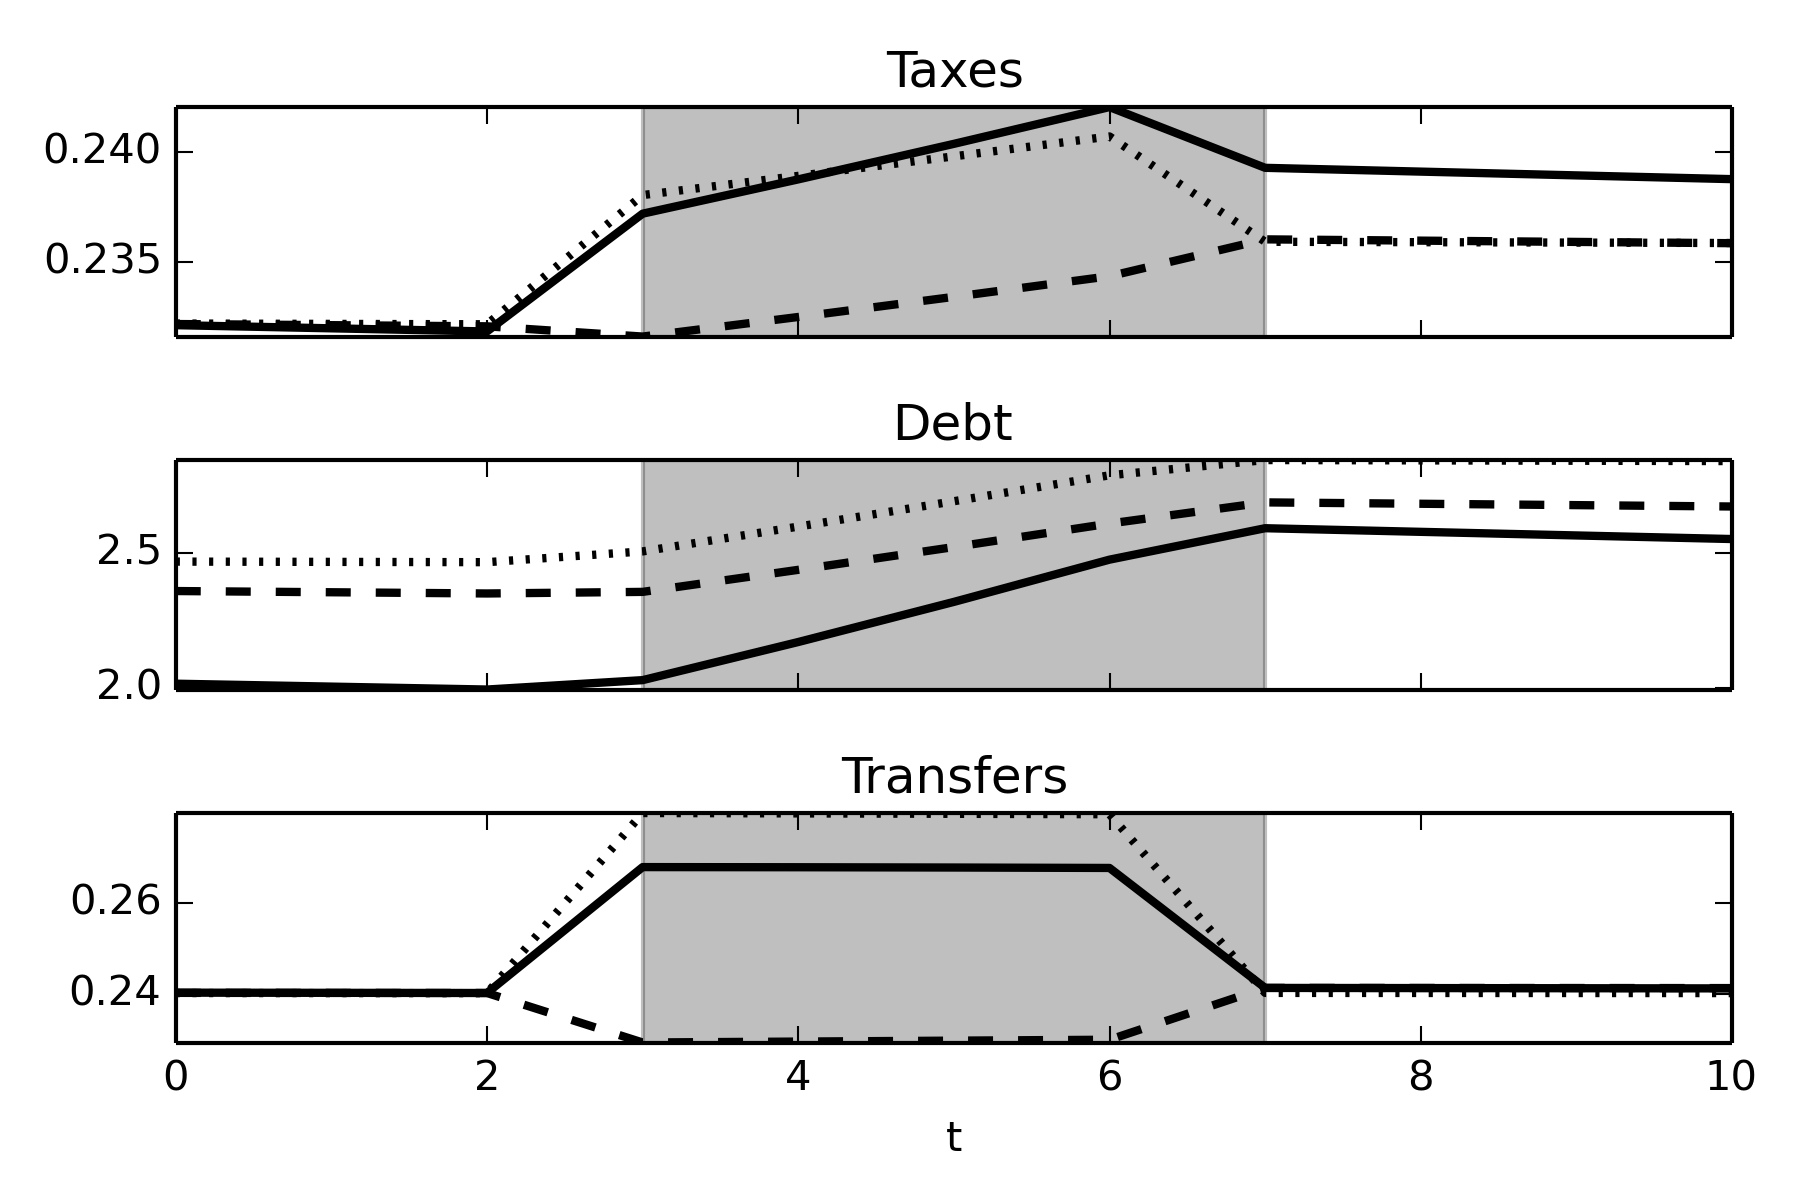
\includegraphics[width = 0.9\textwidth]{cesplots/irf_bm_chi_shocks.png}
    \caption{The bold line is the total response. The dashed (dotted) line reflects the only TFP (inequality) effect. The shaded region is the recession}
  \end{figure}

}
Next we average over sample paths of length 100 periods and report the volatility, autocorrelation, and correlation with exogenous shocks for the  tax rate
and transfers in table \ref{tab:corr}. We see that taxes are twice as volatile and that the correlation between transfers and productivities switches sign.
This  indicates how ignoring redistributive goals affect  prescriptions for government
policy in recessions.

\begin{table}[htp]
\begin{tabular}{|l|l|l|}
\hline
Moments &Tfp& Tfp+Ineq\\\hline
vol. of taxes & 0.003&0.006\\
vol. of transfers &0.01 &0.02\\
autocorr. in taxes& 0.93&0.66\\
autocorr. in transfers& 0.17&0.18\\
corr. of taxes with tfp &0.15 &-0.63\\
corr. of transfers with tfp & 0.99&-0.98\\ \hline
\end{tabular}
\caption{Sample moments for taxes and transfers averaged across simulations of 100 periods}
\label{tab:corr}
\end{table}




\section{Conclusion}
\appendix
\section{Appendix}

\subsection{Extension: Borrowing constraints}\label{Sec: extensions}
%\textcolor{blue}{Anmol : I have removed theorem 2 and addeda mention that the corollary to theorem 1 is valid under adhoc borrowing constraints too. We dont have anything more to say about it. }
%
%\textcolor{blue}{Anmol : I have attempted to re-write the appendix in a way that it is self-contained. The earlier one had forward references and missing arguments.}

Representative agent models  rule out  Ricardian equivalence
either  by assuming distorting taxes or by imposing ad hoc borrowing constraints. %In section \ref{sec:Ricardian101},
By way of contrast, we have verified that Ricardian equivalence holds in our economy even though
there are distorting taxes. % are typically part of an optimal equilibrium.
Imposing ad-hoc borrowing limits also leaves Ricardian equivalence intact in our economy.\footnote{%
\citet{Bryant1984} describe how a government can use borrowing
constraints as part of a welfare-improving policy to finance exogenous
government expenditures. \citet{Sargent1987} describe Modigliani-Miller
theorems for government finance in a collection of economies in which
borrowing constraints on classes of agents produce the kind of rate of
return discrepancies that Bryant and Wallace manipulate.} In economies with
exogenous borrowing constraints, agents' maximization problems  include the
additional constraints
\begin{equation}
b_{i,t}\geq \underline{b}_{i}  \label{borrowing constraint}
\end{equation}%
for some exogenously given $\left\{ \underline{b}_{i}\right\} _{i}.$ %We
%define an equilibrium similarly to Definition \ref{Def: CE with affine taxes}%
\begin{definition}
\label{Def: CE with affine taxes borrowing constraints}For given $\left(
\left \{ b_{i,-1},\underline{b}_{i}\right \} _{i},B_{-1}\right) $ and $%
\left
\{ \tau _{t},T_{t}\right \} _{t},$ a competitive equilibrium with
affine taxes and exogenous borrowing constraints is a sequence $\{ \left \{
c_{i,t},l_{i,t},b_{i,t}\right \} _{i},B_{t},R_{t}\}_{t} $ such that $%
\left
\{ c_{i,t},l_{i,t},b_{i,t}\right \} _{i,t}$ maximizes (\ref{utility
lifetime})\ subject to (\ref{agent bc affine}) and (\ref{borrowing
constraint}), $\{ b_{i,t} \}_{i,t}$ are bounded,
and constraints (\ref{feasibility goods}), (\ref{govmt bc affine})\ and (\ref%
{feasibility bonds})\ are satisfied.
\end{definition}

We can define an \emph{optimal} competitive equilibrium with exogenous borrowing
constraints by extending Definition \ref{Def: optimal CE affine}.

%The role of the initial distribution of assets  is
%unaffected by the introduction of the ad-hoc debt limits and  so is Corollary  \ref{corr: B does not matter}.
The introduction of the ad-hoc debt limits leaves unaltered the conclusions of  Corollary  \ref{corr: B does not matter} and
the role of the initial distribution of assets across agents.
 The next theorem asserts
that ad-hoc borrowing limits do not limit a government's ability to respond to
aggregate shocks.\footnote{%
See \citet{Yared2012,Yared2013}  who shows a closely related result.}
\smallskip

\begin{theorem}
\label{thm:borrowing_constraint}  Given an initial asset distribution $\left(
\left\{ b_{i,-1}\right\} _{i},B_{-1}\right)$, let $\left\{ c_{i,t},l_{i,t}\right\} _{i,t}$ and $\left\{ R_{t}\right\}_t $ be a competitive
equilibrium allocation and interest rate sequence in an economy without
exogenous borrowing constraints. Then for any exogenous
constraints $\left\{ \underline{b}_{i}\right\} _{i}$, there is a government
tax policy $\left\{ \tau _{t},T_{t}\right\} _{t}$ such that $\left\{
c_{i,t},l_{i,t}\right\} _{i,t}$ is a competitive equilibrium
allocation in an economy with exogenous borrowing constraints $\left(
\left\{ b_{i,-1},\underline{b}_{i}\right\} _{i},B_{-1}\right) $ and $\left\{
\tau _{t},T_{t}\right\} _{t}.$
\end{theorem}

\begin{proof}
Let $\left\{ c_{i,t},l_{i,t},b_{i,t}\right\} _{i,t}$
be a competitive equilibrium allocation without exogenous borrowing
constraints. Let $\Delta _{t}\equiv \max_{i}\left\{ \underline{b}%
_{i}-b_{i,t}\right\} .$ Define $\hat{b}_{i,t}\equiv b_{i,t}+\Delta _{t}$ \ for all $t\geq 0$ and $\hat{b}_{i,-1}=b_{-1}.$ By Theorem %
\ref{theorem: main}, $\left\{ c_{i,t},l_{i,t},\hat{b}%
_{i,t}\right\} _{i,t}$ is also a competitive equilibrium allocation without
exogenous borrowing constraints. Moreover, by construction $\hat{b}_{i,t}-%
\underline{b}_{i}=b_{i,t}+\Delta _{t}-\underline{b}_{i}\geq 0$.
Therefore, $\hat{b}_{i,t}$ satisfies (\ref{borrowing constraint}). Since
agents' budget sets are smaller in the economy with exogenous borrowing
constraints, and $\left\{ c_{i,t},l_{i,t},\hat{b}%
_{i,t}\right\} _{i,t}$ are feasible at interest rate process $\left\{
R_{t}\right\} _{t}$, then $\left\{ c_{i,t},l_{i,t},%
\hat{b}_{i,t}\right\} _{i,t}$ is also an optimal choice for agents in the
economy with exogenous borrowing constraints $\left\{ \underline{b}%
_{i}\right\} _{i}.$ Since all market clearing conditions are satisfied, $%
\left\{ c_{i,t},l_{i,t},\hat{b}_{i,t}\right\} _{i,t}$ is a
competitive equilibrium allocation and asset profile.
\end{proof}

To provide some intuition for Theorem \ref{thm:borrowing_constraint}, suppose to the contrary that the exogenous borrowing constraints  restricted a  government's
 ability to achieve a desired allocation. That  means that
the government would want to increase  its borrowing
and to repay agents later, which the borrowing constraints prevent. But the government can just reduce
transfers today and increase them tomorrow. That would  achieve the  desired  allocation
without violating the exogenous borrowing constraints.

Welfare can  be strictly higher in an economy  with exogenous
borrowing constraints  relative to an economy without borrowing constraints because  a government might want to
push some agents against their borrowing limits. When agents' borrowing
constraints bind, their shadow interest rates differ from the
common interest rate that unconstrained agents face. When the government rearranges tax
policies to  affect the  interest rate, it affects constrained and unconstrained agents
 differently.  By facilitating
redistribution, this can improve welfare. %In the next several paragraphs, we will formalize this
%intuition.
We next construct an example without any
shocks in which the government can achieve higher welfare by using borrowing
constraints to improve its ability to redistribute.
In this section we construct an example in which the government can achieve
higher welfare in the economy with ad-hoc borrowing limits. We restrict ourselves to a deterministic economy with $g_t=0$, $\beta_t=\beta$ and $I=2$.  Further the utility function over consumption and labor supply $U(c,l)$ is separable in the arguments and satisfies the Inada conditions. The  planners problem can then be written as the following sequence problem
\begin{equation}
	\max_{\{c_{i,t},l_{i,t},b_{i,t},R_t\}_t} \sum_{t=0}^\infty\beta^t\left[\alpha_1U(c_{1,t},l_{1,t}) +\alpha_2 U(c_{2,t},l_{2,t})\right]\label{eq.A_obj}
\end{equation}subject to
\begin{subequations}
\begin{align}
	c_{2,t}+\frac{U_{l2,t}l_{2,t}}{U_{c2,t}}-\left(c_{1,t}+\frac{U_{l1,t}l_{1,t}}{U_{c1,t}}\right) +\frac{1}{R_t}\left( b_{2,t}-b_{1,t}\right)  = b_{2,t-1}-b_{1,t-1}\label{eq.A_imp}\\
	\frac{U_{l1,t}}{\theta_1U_{c1,t}} = \frac{U_{l2,t}}{\theta_2 U_{c2,t}}\label{eq.A_wage}\\
	c_{1,t}+c_{2,t} \leq \theta_1 l_{1,t}+\theta_2 l_{2,t}\label{eq.A_feas}\\
	\left(\frac{U_{ci,t}}{U_{ci,t+1}}-\beta R_t\right)(b_{i,t}-\underline b_i) = 0\label{eq.A_slack}\\
	\frac{U_{ci,t}}{U_{ci,t+1}} \geq \beta R_t\label{eq.A_euler}\\
	b_{i,t}\geq \underline b_i
\end{align}
\end{subequations}  Where $\underline b_i$ is the exogenous borrowing constraint for agent i.  We obtain equation \eqref{eq.A_imp} by eliminating transfers from the budget equations of the households and using the optimality for labor supply decision. Equations \eqref{eq.A_slack} and \eqref{eq.A_euler} capture the inter-temporal optimality conditions modified for possbily binding constraints.

Let $c^{fb}_i$ and $l^{fb}_i$ be the allocation that solves the first best problem, that is maximizing equation \eqref{eq.A_obj} subject to \eqref{eq.A_feas}, and define
\begin{equation}
	Z^{fb}  = c_{2}^{fb}+\frac{U_{l2}^{fb}l_{2}^{fb}}{U_{c2}^{fb}}-\left(c_{1}^{fb}+\frac{U_{l1}^{fb}l_{1}^{fb}}{U_{c1}^{fb}}\right)
\end{equation}and
\begin{equation}
	\tilde b_2^{fb} = \frac{Z^{fb}}{\frac1\beta -1}
\end{equation}  We will assume that the exogenous borrowing constraints satisfy $\underline b_2 = \underline b_1 + \tilde b_2^{fb}$.  We then have the following lemma

\begin{lemma}  If $\tilde b_2^{fb}>(<)0$ and $b_{2,-1}-b_{1,-1} > (<) \tilde b_2^{fb}$ then the planner can implement the first best.
\end{lemma}
\begin{proof}
We will consider the candidate allocation where $c_{i,t} = c^{fb}_i$, $l_{i,t} = l^{fb}_i$, $b_{i,t} = \underline b_i$ and interest rates are given by $R_t = \frac 1{\beta}$ for $t\geq 1$.  It should be clear then that equations \eqref{eq.A_wage} and \eqref{eq.A_feas} are satisfied as a property of the first best allocation.  Equation \eqref{eq.A_slack} is trivially satisfied since the agents are at their borrowing constraints.  For $t\geq 1$ equations \eqref{eq.A_imp} and \eqref{eq.A_euler} are both satisfied by the choice of $R_t = \frac1\beta$ and the first best allocations.  It remains to check that equation \eqref{eq.A_imp} is satisfied at time $t=0$ for an interest rate $R_0 <\frac1\beta$.  At time zero the constraint is give by
\begin{equation}
	Z^{fb} + \frac 1{R_0} \tilde b^{fb}_2 = b_{2,-1}-b_{1,-1}
\end{equation}  The assumption that $b_{2,-1}-b_{1,-1} > (<) \tilde b_2^{fb}$ if  $\tilde b_2^{fb}>(<)0$ then implies that
\[
	R_ 0 = \frac{\tilde b^{fb}_2}{b_{2,-1}-b_{1,-1}- Z^{fb}} <\frac 1\beta
\] as desired.
\end{proof}

This will improve upon the planners problem without exogenous borrowing constraints, as first best can only be achieved in this scenario when $b_{2,-1}-b_{1,-1} = \tilde b_2^{fb}$.


\newpage

\subsection{Proof of Theorem \ref{theorem: main}}
\label{appndx: thm RE}
 \begin{proof}
 Let
 \begin{equation}
 \hat{T}_{t}=T_{t} + \left(\hat{b}_{1,t} - b_{1,t}\right) -
 R_{t-1}\left(\hat{b}_{1,t-1} - b_{1,t-1}\right) \text{ for
 all }t\geq 0.  \label{construct That}
 \end{equation}%
 Given  a tax policy $\left \{ \tau _{t},\hat{T}_{t}\right \} _{t},$ the
 allocation $\left \{ c_{i,t},l_{i,t},\hat{b}_{i,t}\right \}_{i,t}$ is a feasible choice for consumer $i$ since it satisfies%
 \begin{eqnarray*}
 c_{i,t}&=&\left( 1-\tau _{t}\right) \theta _{i,t}l_{i,t}+R_{t-1}b_{i,t-1}-b_{i,t}+T_{t}\\
 &=&\left( 1-\tau _{t}\right) \theta _{i,t}l_{i,t}+R_{t-1}\left( b_{i,t-1}-b_{1,t-1}\right) -\left(
 b_{i,t}-b_{1,t}\right) +T_{t}+R_{t-1}b_{1,t-1}-b_{1,t} \\
 &=&\left( 1-\tau _{t}\right) \theta _{i,t}l_{i,t}+R_{t-1}\left( \hat{b}_{i,t-1}-\hat{b}_{1,t-1}\right) -\left( \hat{b%
 }_{i,t}-\hat{b}_{1,t}\right) +T_{t}+R_{t-1}b_{1,t-1}-b_{1,t} \\
  &=&\left( 1-\tau _{t}\right) \theta
 _{i,t}l_{i,t}+R_{t-1}\hat{b}_{i,t-1}-\hat{b}_{i,t}+\hat{T}_{t}.
 \end{eqnarray*}%
 Suppose that $\left \{ c_{i,t},l_{i,t},\hat{b}_{i,t}\right \}_{i,t}$ is not the optimal choice for consumer $i$, in the sense that there exists some
 other sequence $\left \{ \hat{c}_{i,t},\hat{l}_{i,t},\hat{b}_{i,t}\right \}_{t}$ that gives strictly higher utility.  Then the choice $%
 \left \{ \hat{c}_{i,t},\hat{l}_{i,t},b_{i,t}\right \}_{t}$ is
 feasible given the tax rates  $\left \{ \tau _{t},T_{t}\right \} _{t}$%
 , which contradicts the assumption that $\left \{ c_{i,t},l_{i,t},b_{i,t}\right \}_{t}$ is the optimal choice for
 the consumer given taxes $\left \{ \tau _{t},T_{t}\right \}
 _{t}$. The new allocation satisfies all other constraints and
 therefore is an equilibrium.
 \end{proof}
\newpage

\subsection{Proof of Theorem \ref{prop: affine eqm nec and suff}}
\label{appndx: affine eqm nec and stuff}
\smallskip

We prove a slight more general version of our result. Consider an infinite
horizon, incomplete markets economy in which an agent maximizes utility
function $U:\mathbb{R}_{+}^{n}\rightarrow \mathbb{R}$ subject to an infinite
sequence of budget constraints. We assume that $U$ is concave and
differentiable. Let $\mathbf{x}(s^t)$ be a vector of $n$ goods and let $%
\mathbf{p}(s^{t})$ be a price vector in state $s^{t}$ with $p_{i}(s^{t})$
denoting the price of good $i.$ We use a normalization $p_{1}\left(
s^{t}\right) =1$ for all $s^{t}.$ 
Let $b(s^{t})$ be the agent's asset holdings, and let $\mathbf{e}\left(
s^{t}\right) $ be a stochastic vector of endowments.

\textbf{Consumer maximization problem}

\begin{equation}
\max_{\mathbf{x}_{t},b_{t}}\sum_{t=0}^{\infty }\beta ^{t}\Pr \left(
s^{t}\right) U(\mathbf{x}\left( s^{t}\right) )
\label{Tech appendix: consumer maximization}
\end{equation}%
subject to%
\begin{equation}
\label{Tech appendix: budget constraint}
\mathbf{p}\left( s^{t}\right) \mathbf{x}\left( s^{t}\right) +q(s^{t})b\left(
s^{t}\right) =\mathbf{p}\left( s^{t}\right) \mathbf{e}\left( s^{t}\right)
+P(s_t)b\left( s^{t-1}\right) 
\end{equation}%
and $\left \{ b\left( s^{t}\right) \right \} $ is bounded and $\left \{
q(s^{t})\right \} $ is the price of the risk-free bond.

The Euler conditions are%
\begin{eqnarray}
\mathbf{U}_{x}(s^{t}) &=&U_{1}(s^{t})\mathbf{p}(s^{t})
\label{Tech appendix: Euler} \\
\Pr \left( s^{t}\right) U_{1}\left( s^{t}\right) q(s^{t}) &=&\beta
\sum_{s^{t+1}>s^{t}}\Pr \left( s^{t+1}\right) U_{1}\left( s^{t+1}\right) .
\notag
\end{eqnarray}

\begin{theorem}

\smallskip Consider an allocation $\left \{ \mathbf{x}_{t},b_{t}\right \} $
that satisfies (\ref{Tech appendix: budget constraint}), (\ref{Tech
appendix: Euler}) and $\left \{ b_{t}\right \} _{t}$ is bounded. Then $%
\left
\{ \mathbf{x}_{t},b_{t}\right \} $ is a solution to (\ref{Tech
appendix: consumer maximization}).

\end{theorem}
\begin{proof}
The proof follows closely Constantinides and Duffie (1996). Suppose there is
another budget feasible allocation $\mathbf{x}+\mathbf{h}$ that maximizes (%
\ref{Tech appendix: consumer maximization}). Since $U$ is strictly concave,
\begin{eqnarray}
&&\mathbb{E}_{0}\sum_{t=0}^{\infty }\beta ^{t}U(\mathbf{x}_{t}+\mathbf{h}%
_{t})-\mathbb{E}_{0}\sum_{t=0}^{\infty }\beta ^{t}U(\mathbf{x}_{t})
\label{Tech appendix: gain from h} \\
&\leq &\mathbb{E}_{0}\sum_{t=0}^{\infty }\beta ^{t}\mathbf{U}_{x}(\mathbf{x}%
_{t})\mathbf{h}_{t}  \notag
\end{eqnarray}

To attain $\mathbf{x}+\mathbf{h}$, the agent must deviate by $\varphi _{t}$
from his original portfolio $b_{t}$ such that $\left\{ \varphi _{t}\right\}
_{t}$ is bounded$,$ $\varphi _{-1}=0$ and
\begin{equation*}
\mathbf{p}(s^{t})\mathbf{h}\left( s^{t}\right) =P(s_t)\varphi
(s^{t-1})-q(s^{t})\varphi (s^{t})
\end{equation*}%
Multiply by $\beta ^{t}\Pr \left( s^{t}\right) U_{1}(s^{t})$ to get:%
\begin{eqnarray*}
\beta ^{t}\Pr \left( s^{t}\right) U_{1}(s^{t})\mathbf{p}(s^{t})\mathbf{h}%
\left( s^{t}\right)  &=&\beta ^{t}\Pr \left( s^{t}\right)
U_{1}(s^{t})\varphi (s^{t-1})-q(s^{t})\beta ^{t}\Pr \left( s^{t}\right)
U_{1}(s^{t})\varphi (s^{t}) \\
&=&\beta ^{t}\Pr \left( s^{t}\right) U_{1}(s^{t})\varphi (s^{t-1})-\beta
^{t+1}\sum_{s^{t+1}>s^{t}}\Pr \left( s^{t+1}\right) U_{1}\left(
s^{t+1}\right) \varphi (s^{t})
\end{eqnarray*}%
where we used the second part of (\ref{Tech appendix: Euler}) in the second
equality. Sum over the first $T$ periods and use the first part of (\ref%
{Tech appendix: Euler}) to eliminate $\mathbf{U}_{x}(\mathbf{x}%
_{t})=U_{1}(s^{t})\mathbf{p}(s^{t})$%
\begin{equation*}
\sum_{t=0}^{T}\beta ^{t}\Pr \left( s^{t}\right) \mathbf{U}_{x}(\mathbf{x}%
_{t})\mathbf{h}\left( s^{t}\right) =-\sum_{s^{T+1}>s^{T}}\beta ^{T+1}\Pr
\left( s^{T+1}\right) U_{1}\left( s^{T+1}\right) \varphi (s^{T}).
\end{equation*}%
Since $\left\{ \varphi _{t}\right\} _{t}$ is bounded there must exist $\bar{%
\varphi}$ s.t. $|\varphi _{t}|\leq \bar{\varphi}$ for all $t$. By Theorem
5.2 of Magill and Quinzii (1994), this equilibrium with debt constraints
implies a transversality condition on the right hand side of the last
equation, so by transitivity we have%
\begin{equation*}
\lim_{T\rightarrow \infty }\sum_{t=0}^{T}\beta ^{t}\Pr \left( s^{t}\right)
\mathbf{U}_{x}(\mathbf{x}_{t})\mathbf{h}\left( s^{t}\right) =0.
\end{equation*}%
Substitute this into (\ref{Tech appendix: gain from h}) to show that $%
\mathbf{h}$ does not improve utility of consumer.
\end{proof}
\newpage

\subsection{Proof of Theorem \protect\ref{thm: rep agent general theorem}}


\begin{proof}
The optimal Ramsey plan solves the following Bellman equation. Let $V(b\_)$ be the maximum ex-ante value the government can achieve with debt $b\_$. 

\begin{equation}
  \label{eq-QLRA obj}
    V(b\_)=\max_{c(s),l(s),b(s)} \sum_{s}\pi(s)\left\{c(s)-\frac{l(s)^{1+\gamma}}{1+\gamma}+\beta V(b(s)) \right\}
\end{equation}   
subject to

   \begin{subequations}
   \label{sys- QLRA constraint}
    \begin{equation}
    \label{rep agent implementability constraint }
    c(s)+b(s)=l(s)^{1+\gamma}+\beta^{-1} P(s)b\_
    \end{equation}
 

 
\begin{equation}
  \label{eq-resoruces}
c(s)+g(s)\leq\theta l(s)
\end{equation}   
Let $\bar{b}=-\underline{B}$
\begin{equation}
  \label{ndl}
\underline{b}\leq b(s)\leq \bar{b}
\end{equation}   


   \end{subequations}
%Let $\mu(s)\pi(s),\phi(s)\pi(s)$ be the Lagrange multipliers on the respective constraints. 

Let $\mu(s),\phi(s),\underline{\kappa}(s),\overline \kappa(s) $ be the Lagrange multipliers on the respective constraints.
\noindent {Part 1 of Theorem \textbf{\ref{thm: rep agent general theorem}}}

\begin{lemma}
There exists  a $\overline{b}$ such that $b_t\leq\overline{b}$. This is the natural debt limit for the government.
\end{lemma}
\begin{proof}
As we drive $\mu$ to $-\infty$, the tax rate approaches a maximum limit, $\bar{\tau}=\frac{\gamma}{1+\gamma}$. In state $s$, the government surplus,
\[
  S(s,\tau) = \theta^\frac\gamma{1+\gamma}(1-\tau)^\frac1\gamma\tau - g(s),
\]  which  is  maximized at $\tau = \frac\gamma{1+\gamma}$ when $(1-\tau)^\frac1\gamma\tau$ is also maximized. This would impose a natural borrowing limit for the government. 

\end{proof}

From now we assume that $\overline{b}$ represents the natural borrowing limit. We begin with some useful lemmas

let $L\equiv l^{1+\gamma }$, to make this problem convex, 

Substitute for $c\left( s\right) $%
\[
V\left( b\_\right) =\max_{L(s),b(s)}\sum_{s\in S}\pi \left(
s\right) \left[ \frac{1}{1+\gamma }L\left( s\right) +\frac{1}{\beta }%
P\left( s\right) b\_-b\left( s\right) +\beta V\left( b\left( s\right)
\right) \right] 
\]%
s.t.%
\begin{eqnarray*}
\frac{1}{\beta }P\left( s\right) b-b\left( s\right) +g\left( s\right) &\leq
&\theta L^{\frac{1}{1+\gamma} }\left( s\right) -L\left( s\right) \\
b\left( s\right) &\leq &\bar{b} \\
L\left( s\right) &\geq &0.
\end{eqnarray*}

\begin{lemma}
\smallskip $V\left( b\right) $ is stictly concave, continuous,
differentiable and $V\left( b\right) <\beta ^{-1}$ for all $%
b<\bar{b}.$ The feasibility constraint binds for all $b\in (-\infty ,\bar{b}%
],\ s\in S$ and $\left( L^{\ast }\left( s\right) \right) ^{1-\frac{1}{1+\gamma} }\geq
\frac{1}{1+\gamma} .\footnote{
This last condition simply means that we do not tax to the right of the peak
of the Laffer curve. The revenue maximizing tax is $1-\bar{\tau}=\frac{1}{%
1+\gamma }.$ At the same time $1-\tau =l^{\gamma}$ so if taxes are always
to the left of the peak, $\frac{1}{1+\gamma }\leq l^{\gamma }=\left(
L^{\frac{1}{1+\gamma} }\right) ^{\gamma}=L^{1-\frac{1}{1+\gamma} }$.}$ 
\end{lemma}

\begin{proof}
\smallskip \textit{Concavity}

$V\left( b\right) $ is concave because we maximize linear objective
function over convex set.

\textit{Binding feasibility}

Suppose that feasibility does not bind for some $b,s.$ Then the optimal $%
L\left( s\right) $ solve $\max_{L\left( s\right) \geq 0}\pi \left( s\right) 
\frac{\gamma}{1+\gamma }L\left( s\right) $ which sets $L\left( s\right)
=\infty .$ This violates feasility for any finite $b,b\left( s\right) .$

\textit{Bounds on }$L$

Let $\phi\left( s\right) >0$ be a Lagrange multiplier on the
feasibility. \ The FOC for $L\left( s\right) $ is 
\[
\frac{1}{1+\gamma }+\phi(s) \left( \frac{1}{1+\gamma }L(s)^{\frac{1}{1+\gamma}
-}-\theta \right) =0. 
\]%
This gives%
\[
\frac{1}{1+\gamma }L^{\frac{1}{1+\gamma} -1}-\theta =-\frac{1}{\lambda }\frac{\gamma}{%
1+\gamma }<0 
\]%
or%
\[
L^{1-\frac{1}{1+\gamma} }\geq \frac{\theta }{1+\gamma }. 
\]

\textit{Continuity}

For any $L$ that satisfy $L^{1-\frac{}{1+\gamma} }\geq \frac{\theta }{1+\gamma} ,$ define function $%
\Psi $ that satisfies $\Psi \left( L^{\frac{1}{1+\gamma} }-\theta L\right) =L.$ Since $%
L^{\frac{1}{1+\gamma} }-L$ is strictly decreasing in $L$ for $L^{1-\frac{1}{1+\gamma} }\geq
\frac{1}{1+\gamma} $, this function is well defined. Note that $\Psi \left(
{}\right) \underbrace{\left( \frac{1}{1+\gamma }L^{\frac{1}{1+\gamma} -1}-\theta \right) }%
_{<0}=1$ (so that $\Psi >0$, i.e. $\Psi $ is strictly decreasing)
and $\Psi ^{\prime \prime }\underbrace{\left( \frac{1}{1+\gamma }L^{\frac{1}{1+\gamma}
-1}-1\right) ^{2}}_{>0}+\underbrace{\Psi }_{<0}\underbrace{\frac{1%
}{1+\gamma }\frac{\gamma }{1+\gamma }L^{\frac{1}{1+\gamma} -2}}_{<0}=0$ (so that $\Psi
^{\prime \prime }\geq 0$, $\Psi ^{\prime \prime }>0,$ i.e. $\Psi $ is
strictly concave on the interior). $\Psi $ is also continuous. When $%
L^{1-\frac{1}{1+\gamma} }=\frac{1}{1+\gamma} ,$ $L=(1+\gamma) ^{-\frac{(1+\gamma)} {\left( \gamma \right)} }.$
Let $D\equiv (1+\gamma) ^{\frac{-1}{ \gamma }-(1+\gamma) ^{-\frac{1+\gamma }{\left(\gamma\right)} }}.$ Then the objective is 
\[
V\left( b\_\right) =\max_{b\left( s\right) }\sum_{s\in S}\pi \left(
s\right) \left[ \Psi \left( \frac{1}{\beta }P\left( s\right) b-b\left(
s\right) +g\left( s\right) \right) +\frac{1}{\beta }P\left( s\right)
b\_-b\left( s\right) +\beta V\left( b\left( s\right) \right) \right] 
\]%
s.t.%
\begin{eqnarray*}
b\left( s\right) &\leq &\bar{b} \\
\frac{1}{\beta }P\left( s\right) b\_-b\left( s\right) +g\left( s\right) &\leq
&D.
\end{eqnarray*}

This function is continuous so $V$ is also continuous.

\textit{Differentiability}

Continuity and convexity implies differentiability everywhere, including the
boundaries.

\textit{Strict concavity}

$\Psi $ is strictly concave, so on the interior $V$ is strictly
concave.

\end{proof}

\smallskip Next we characterize policy functions

\begin{lemma}
\label{lem increasing b}
$b\left( s,b\_\right) $ is an increasing function of $b$ for all $s$ for all $%
s,b\_ $ where $b\left( s\right) $ is interior.
\end{lemma}

\begin{proof}
Take the FOCs for $b\left( s\right) $ from the condition in the previous
problem. If $b\left( s\right) $ is interior%
\[
\Psi \left( \frac{1}{\beta }P\left( s\right) b\_-b\left( s\right)
+g\left( s\right) \right) =\beta V\left( b\left( s\right)
\right) . 
\]

Suppose $b_{1}<b_{2}$ but $b_{2}\left( s\right) <b_{1}\left( s\right) .$
Then from stict concavity%
\begin{eqnarray*}
V\left( b_{2}\left( s\right) \right) &<&V^{\prime
}\left( b_{1}\left( s\right) \right) \\
\Psi \left( \frac{1}{\beta }P\left( s\right) b_{2}-b_{2}\left(
s\right) +g\left( s\right) \right) &>&\Psi \left( \frac{1}{\beta }%
P\left( s\right) b_{1}-b_{1}\left( s\right) +g\left( s\right) \right) .
\end{eqnarray*}
\end{proof}

\begin{lemma}
There exists an invariant distribution of the stochastic process $b_{t+1}=b(s_{t+1},b_t)$ 
\end{lemma}
\begin{proof}
The state spaces for $b_t$ and $s_t$ are compact. Further the transition function on $s_{t+1}|s_{t}$ is trivially increasing under i.i.d shocks. We can apply standard arguments as in \cite{Prescott1992}(see corollary 3) to argue that there exists invariant distribution of assets.  
\end{proof}

Now we characterize the support of this distribution using further properties of the policy rules for $b(s|b\_)$


\begin{lemma}
\label{prop: b(s) relative to b}For any $b\_\in (\underline{b} ,\bar{b}),$ there are $s,s^{\prime \prime }$ s.t. $b\left( s\right) \geq b\_\geq b\left( s^{\prime \prime }\right) .$ Moreover, if there are any states $s^{\prime \prime },s^{\prime \prime \prime }$ s.t. $b\left( s^{\prime \prime
}\right) \neq b\left( s^{\prime \prime \prime }\right) ,$ those inequalities
are strict.
\end{lemma}


\begin{proof}
The FOCs together with the envelope theorem imply that $\mathbb{E}P(s)V'(b(s))=V'(b\_)+\kappa(s)$
We can rewrite this as $\mathbb{\tilde{E}}V'(b(s))=b+\kappa(s)$ with $\tilde{\pi}(s)=P(s)\pi(s)$

Now if there is at least one $b\left( s\right) $ s.t. $b\left(
s\right) >b\_,$ by strict concavity of $V$ there must be some $%
s^{\prime \prime }$ s.t. $b\left( s^{\prime \prime }\right) <b.$

If there is at least one $b\left( s\right) $ s.t. $b\left(
s\right) <b\_,$ the inequality above is strictly only if $b\left(
s^{\prime \prime \prime }\right) =\bar{b}$ for some $s^{\prime \prime \prime
}.$ But $V\left( \bar{b}\right) <V\left(
b\right) $ so there must be some $s^{\prime \prime }$ s.t. $b\left(
s^{\prime \prime }\right) >b.$ Equality is possible only if $b\_=b\left(
s\right) $ for all $s.$
\end{proof}


\begin{lemma}  Let $\mu(b,s)$ be the optimal policy function for the Lagrange multiplier $\mu(s)$.  If $P(s') > P(s'')$ then there exists a $b^*_{s',s''}$ such that for all $b < (>) \; b_{1,s',s''}$ we have $\mu(b,s') > (<) \;\mu(b,s'')$.  If $\underline b < b^*_{s',s''} < \overline b$ then $\mu(b^*_{s',s''},s') = \mu(b^*_{s',s''},s'')$.
\label{lem.order}
\end{lemma}
\begin{proof} 
Suppose that $\mu(b,s')\leq \mu(b,s'')$.  Subtracting the implementability for $s''$ from the implementability constraint for $s'$ we have 
\begin{align*}
	\frac{P(s')-P(s'')}{\beta}b &= S_{s'}(\mu(b,s'))-S_{s''}(\mu(b,s'')) + b'(b,s')-b'(b,s'')\\
						&\geq S_{s'}(\mu(b,s')) -S_{s''}(\mu(b,s')) + b'(b,s')-b'(b,s'')\\
						&\geq  S_{s'}(\mu(b,s')) -S_{s''}(\mu(b,s')) = g(s'')-g(s')
\end{align*}  We get the first inequality from noting that $S_s(\mu')\geq S_s(\mu'')$ if $\mu' \leq \mu''$.  We obtain the second inequality by noting that $\mu(b,s')\leq \mu(b,s'')$ implies $b'(b,s')\geq b'(b,s'')$ (which comes directly from the concavity of $V$).
Thus, $\mu(b,s')\leq \mu(b,s'')$ implies that 
\begin{equation}
\label{pair-wise ss}
b \geq \frac{\beta(g(s'')-g(s'))}{P(s')-P(s'')} = b^*_{s',s''} 
\end{equation}

The converse of this statement is that if $b<b^*_{s',s''}$ then $\mu(b,s') > \mu(b,s'')$.  The reverse statement that $\mu(b,s') \geq \mu(b,s'')$ implies $b \leq b^*_{s,s'}$ follows by symmetry.   Again, the converse implies that if $b > b^*_{s',s''}$ then $\mu(b,s') < \mu(b,s'')$.    Finally, if $\underline b < b^*_{s',s''} <\overline b$ then continuity of the policy functions implies that there must exist a root of $\mu(b,s')-\mu(b,s'')$ and that root can only be at $b^*_{s',s''}$.
\end{proof}


\begin{lemma}
\label{lem: existence and uniqueness of ss}
$P \in \mathcal{P}^*$ is necessary and sufficient for existence of $b^*$ such that $b(s,b^*)=b^*$ for all $s$s
\end{lemma}

\begin{proof}
The necessary part follows from taking differences of the \eqref{rep agent implementability constraint } for $s'$,$s''$. We have 
\[[P(s)-P(s'')]\frac{b^*}{\beta}=g(s)-g(s'')\]
Thus $P\in\mathcal{P}^*$. The sufficient part follows from the Lemma \ref{lem.order}. If $P \not \in \mathcal{P}^*$, equation \eqref{pair-wise ss} that defines $b^*_{s',s''}$ will not be same across all pairs. Thus $b^*$ that satisfies $b(s;b^*)$ independent of $s$ will not exist.
\end{proof}


Lemma  \ref{lem: existence and uniqueness of ss}  implies that under the hypothesis of part 1 of the Theorem \ref{thm: rep agent general theorem} there cannot exist an interior absorbing point for the dynamics of debt. This allows us to construct a sequences $\{b_t\}_t $ such that $b_t<b_{t+1}$ with the property that $\lim_tb_t=\underline{b}$.
Thus, for any $\epsilon>0$, there exists a finite history of shocks that can take us arbitrarily close to $\underline{b}$. Since the shocks are i.i.d this finite sequence will repeat i.o. With a symmetric argument we can show that $b_t$ will come arbitrarily close to its upper limit i.o too





{Part 2 of Theorem \textbf{\ref{thm: rep agent general theorem}}}


In this first section we will show that there exists $b_1$, and if $P(s)$ is sufficiently volatile a $b_2$, such that if $b_t\leq b_1$ then 
\[
	\mu_t \geq \EE_t \mu_{t+1}
\] and if $b_t \geq b_2$ then
\[
	\mu_t \leq \EE_t \mu_{t+1}.
\]  Recall that $b$ is decreasing in $\mu$, so this implies that if $b_t$ is low (large) enough then there will exist a drift away from the lower (upper) limit of government debt.

With Lemma \ref{lem.order} we can order the policy functions $\mu(b,\cdot)$ for particular regions of the state space.  Take $b_1$ to be
\[
	b_1 = \min\left\{b^*_{s',s''}\right\}
\] and WLOG choose $\underline b < b_1$.  For all $b < b_1$ we have shown that $P(s) > P(s')$ implies that $\mu(b,s) > \mu(b,s')$.  The FOC for the problem imply,

\begin{equation}\label{eq.mart}
	\mu\_ = \EE P(s)\mu(s)+\underline{\kappa}(s)
\end{equation}  The inequality in the resource constraint implies that $\phi(s)\geq 0$ implying that $\mu(s) \leq 1$.  With some minor algebra algebra we obtain

By decomposing $\EE \mu(s)P(s)$ in equation \eqref{eq.mart}, we obtain (using $\EE P(s) = 1$)
\begin{equation}
	\mu\_ = \EE\mu(s) +\cov (\mu(s),P(s)) + \underline \kappa(s)
\end{equation}Our analysis has just shown that for $b\_ < b_1$ we have $\cov_t (\mu(s),P(s))  >0$ so 
\[
	\mu\_> \EE\mu(s).
\]  If $p$ is sufficiently volatile:
\[
	P(s') - P(s'') > \frac{\beta(g(s'')-g(s'))}{\overline b}
\] then 
\[
	b_2 = \max\left\{b^*_{s',s''}\right\} <\overline b
\] and through a similar argument  we can conclude that $\cov(\mu(s),P(s)) < 0$ 
\[
	\mu\_ < \EE \mu (s)
\] for $b\_ > b_2$ (note $b\_ >\underline b$ implies $\underline \kappa(s) =0$) which gives us a drift away from the upper-bound. 


{Part 3 of Theorem \textbf{\ref{thm: rep agent general theorem}}}


When $P\in\mathcal{P}^*$, Lemma \ref{lem: existence and uniqueness of ss} implies existence of $b^*$ as the steady state debt level.
\begin{lemma}
\label{sub super martingale}
There exists $\mu^*$ such that $\mu_t$  is a sub-martingale bounded above in the region $(-\infty,\mu^*)$ and super-martingale bounded below in the region $(\mu^*,\frac{1}{1+\gamma})$


\end{lemma}
\begin{proof}
Let $\mu^*$ be the associated multiplier, i.e $V_b(b^*)=\mu^*$.  Using the results of the previous section, we have that $b_1 = b_2 = b^*$, implying that $\mu_t < (>) \EE_t\mu_{t+1}$ for $b_t  < (>) b^*$. 
\end{proof}

Lastly we show that $\lim_t \mu_t=\mu^*$. Suppose $b_{t}<b^*$, we know that $\mu_t>\mu^*$. The previous lemma implies that in this region, $\mu_t$ is a super martingale. The lemma $\ref{lem increasing b}$ shows that $b(s,b\_)$ is continuous and increasing. This translates into $\mu(\mu(b\_),s)$ to be continuous and increasing as well.
 Thus 
 \[\mu_{t}>\mu^* \implies \mu(\mu_{t},s_{t+1})>\mu(\mu^*,s_{t+1}) \]
or
 \[\mu_{t+1}>\mu^*\]
Thus $\mu*$  provides a lower bound to this super martingale. Using standard martingale convergence theorem converges. The uniqueness of steady state implies that it can only converge to $\mu^*$. For $\mu<\mu^*$, the argument is symmetric.


\end{proof}

\newpage

\subsection{Proof of Theorem \protect\ref{thm: rep agent linear policies}}
\label{appndx: ergodic distribution linearization}
Working with the first order conditions of problem \ref{eq-QLRA obj}, we obtain
\[
	l(s)^\gamma = \frac{\mu(s)-1}{(1+\gamma)\mu(s) - 1} = 1-\tau(\mu(s)),
\]
implying the relationship between tax rate $\tau$ and multiplier $\mu$ given by

\begin{equation}\label{eq.tau}
	\tau(\mu) = \frac{\gamma\mu}{(1+\gamma)\mu-1}
\end{equation}

At the interior, the rest of the first order conditions  and the implementability constraints are summarized below
\begin{align*}
	\frac{b\_ P(s)}{\beta }= S(\mu(s),s) + b(s)\\
	\mu(b\_) = \EE P(s) \mu(s)\\
\end{align*} 

where $S(\mu,s)$ is the government surplus in state $s$ given by
\[
	S(\mu,s) = (1-\tau(\mu))^\frac1\gamma \tau(\mu)-g(s) = I(\mu) - g(s)
\]


The proof of the theorem will have four steps:

\textbf{Step 1:} Obtaining a recursive representation of the optimal allocation in the incomplete markets economy with payoffs $P(s)$ with state variable $\mu\_$


Given a pair $\{P(s),g(s)\}$, since $V'(b)$ is one-to-one, so we can re-characterize these equations as searching for a function $b(\mu)$ and $\mu(s|\mu\_)$such that the following two equations can be solved for all $\mu\_$.
\begin{align}\label{eq.lin_imp}
	\frac{b(\mu\_)P(s)}{\beta } = I(\mu(s)) - g(s) +b(\mu(s))\\
	\mu\_ = \EE\mu(s)P(s)\label{eq.lin_mart}
\end{align}  



\textbf{Step 2:} Describe how the policy rules are approximated

Usually perturbation approaches  to solve equilibrium conditions as above look for the solutions to $\{\mu(s|\mu\_)\}$ and $b(\mu\_)$ around deterministic steady state of the model. Thus for any $b^{ss}$, there exists a $\mu^{ss}$ that will solve

\[	\frac{b^{SS}}{\beta } = I(\mu^{SS}) - \bar{g} +b^{SS}\\
\]


For example if we set the perturbation parameter $q$ to scale the shocks, $g(s)=\mathbb{E}g(s)+q\Delta_g(s)$ and $P(s)=1+q\Delta_{P}(s)$, the first order expansion of $\mu(s|\mu\_)$ will imply that it is a martingale. Such approximations are not informative about the ergodic distribution. \footnote{One can do higher order approximations, but part 3 of theorem \ref{thm: rep agent general theorem} hints that for economies with payoffs close to $\mathcal{P}^*$, the stochastic steady state in general is far away from $\mu^{SS}$.}



In contrast we will approximate the functions $\mu(s|\mu\_)$ around 
around economy with payoffs in $\bar{P}\in \mathcal{P}^*$. 

In contrast we a) explicitly recognize that policy rules depend on payoffs: $\mu(s|\mu\_,\{P(s)\}_s)$ and $b(\mu\_,\{P(s)\}_s)$ and then take take the first order expansion with respect to both $\mu\_$ and $\{P(s)\}$ around the vector $(\bar{\mu},\{\bar{P}(s)\}_s)$ where $\bar{P}(s) \in \mathcal{P}^*$: these payoffs support  an allocation such that limiting distribution of debt is degenerate around the some value $\bar{b}$; and  $\overline {\mu}$ is the corresponding limiting value of multiplier. The next two expression make the link between $\bar{\mu}$ and $\bar{b}$ explicit. 
\begin{subequations}
\label{eq.ss.} 
\begin{equation}
\overline b = \frac{\beta}{1-\beta}\left( I(\overline\mu) - \overline g\right) 
\end{equation}
where $\overline g = \EE g$ and $\overline p$ as 
\begin{equation}
	\overline P(s) = 1- \frac\beta{\overline b}(g(s) - \overline g) 
\end{equation}
\end{subequations}

As noted before $b(\overline\mu;\overline p) = \overline b$ solves the the system of equations (\ref{eq.lin_imp}-\ref{eq.lin_mart}) for $\mu'(s) = \overline \mu$ when the payoffs are $\overline{P}(s)$ 

We next obtain the expressions that characterize the linear approximation of $\mu(s|\mu\_,\{P(s)\})$ and $\b(\mu\_,\{P(s)\})$ around some arbitrary point $(\bar{\mu},\{\bar{P}(s)\}_s)$ where $\bar{P}(s) \in \mathcal{P}^*$. We will use these expressions to compute the mean and variance of the ergodic distribution associated with the approximated policy rules. Finally as a last step we propose a particular choice of the point of approximation.

The derivatives $\frac{\delta \mu(s|\mu\_,\{P(s)\}}{\delta \mu\_}$,$\frac{\delta \mu(s|\mu\_,\{P(s)\}}{\delta P(s)}$ and similarly for  $b(\mu\_,\{P(s)\}$ are obtained below:


Differentiating equation \eqref{eq.lin_imp} with respect to $\mu$ around $(\overline \mu,\overline P)$ we obtain
\[
	\frac{\overline{P}(s)}{\beta}\frac{\partial b}{\partial \mu\_} = \left[I'(\mubar)+\frac{\partial b}{\partial \mu\_}\right]\frac{\partial \mu(s)}{\partial \mu\_}.
\]Differentiating equation \eqref{eq.lin_mart} with respect to $\mu\_$ we obtain
\[
	1 = \sum_{s} \pi(s) \overline P(s) \frac{\partial \mu'(s)}{\partial \mu\_}
\]combining these two equations we see that 
\[
	\frac1\beta\left(\sum_s\pi(s)\overline P(s)^2\right)\frac{\partial b}{\partial \mu\_} = I'(\mubar) + \frac{\partial b}{\partial \mu\_}
\]Noting that $\EE\overline P^2(s) = 1 + \frac{\beta^2}{\bbar^2}\sigma^2_g$ we obtain
\begin{equation}
	\frac{\partial b}{\partial \mu\_} = \frac{I'(\mubar)}{\frac{\beta}{\bbar^2}\sigma_g^2 +\frac{1-\beta}{\beta}} < 0
\end{equation}as $I'(\mubar) < 0$.  We then have directly that 
\begin{equation}
	\frac{\partial \mu'(s)}{\partial \mu} = \frac{\overline P(s)}{\frac{\beta^2}{\overline b^2}\sigma^2_g +1} = \frac{\overline P(s)}{\EE\overline P(s)^2}
\end{equation}  We can perform the same procedure for $P(s)$.  Differentiating equation \eqref{eq.lin_imp} with respect to $P(s)$ we around $(\mubar,\pbar)$ we obtain
\begin{equation}\label{eq.dimp_dps}
\frac{\pbar(s')}{\beta}\frac{\partial b}{\partial P(s)} + 1_{s,s'}\frac{\bbar}{\beta} - \frac{\pi(s)\bbar\pbar(s')}{\beta} = \left[I'(\mubar) + \frac{\partial b}{\partial \mu}\right]\frac{\partial \mu(s')}{\partial P(s)}
\end{equation} Here $1_{s,s'}$ is $1$ if $s = s'$ and zero otherwise.  Differentiating equation \eqref{eq.lin_mart} with respect to $P(s)$ we obtain
\[
	0 = \pi(s)\overline \mu - \pi(s)\overline \mu + \sum_{s'} \pi(s) \pbar(s')\frac{\partial \mu(s')}{\partial P(s)} =  \sum_{s'} \pi(s')\pbar(s')\frac{\partial \mu(s')}{\partial P(s)}
\]  Again we can combine these two equations to give us
\[
	\frac{\EE\pbar(s)^2}{\beta}\frac{\partial b}{\partial P(s)} + \frac{\pi(s)\bbar}{\beta}(\pbar(s)-\EE\pbar(s)^2) = 0
\] or
\begin{equation}
	\frac{\partial b}{\partial P(s)} = \pi(s)\bbar \frac{\EE\pbar^2-\pbar(s)}{\EE\pbar^2}
\end{equation}Going back to equation \eqref{eq.dimp_dps} we have
\begin{equation}
	\frac{\partial \mu(s')}{\partial P(s)} = \frac{\bbar}{\beta\left[I '(\mubar) + \frac{\partial b}{\partial \mu}\right]}\left(1_{s,s'}-\frac{\pi(s)\pbar(s)\pbar(s')}{\EE\pbar^2}\right)
\end{equation}


\textbf{Step 3:} Getting expressions for the mean and variance of the ergodic distribution around some arbitrary point of approximation

For an arbitrary $\left (\overline \mu,\{\overline {P}(s )\}_{s}\right)$, using the derivatives that we computed, we can characterize the dynamics of $\hat{\mu}\equiv\mu_t-\mubar$ using our approximated policies.


\[
	\hat \mu_{t+1} = B(s_{t+1}) \hat\mu_t + C(s_{t+1}),
\]  where $B(s)$ and $C(s)$ are respective derivatives. Note that both are random variables and let us denote their means $\barB$ and $\barC$, and variances $\sigma_B^2$ and $\sigma_C^2$ .  Suppose that $\hat\mu$ is distributed according to the ergodic distribution of this linear system with mean $\EE\hat\mu$ and variance $\sigma^2_\mu$.  Since 
\[
	B\hat\mu +C,
\]has the same distribution we can compute the mean of this distribution as
\[
\begin{split}
	\EE\hat\mu &= \EE\left[ B\hat\mu+C\right]\\
			  &= \EE\left[\EE_{\hat\mu}\left[B\hat\mu+C\right]\right]\\
			  &= \EE\left[\barB\hat\mu +\barC\right]\\
			  &=\barB\EE\hat\mu+\barC
\end{split}
\]solving for $\EE\hat\mu$ we get
\begin{equation}
	\EE\hat\mu = \frac{\barC}{1-\barB}
\end{equation}For the variance $\sigma^2_{\hat\mu}$ we know that 
\[
	\sigma^2_{\hat\mu} = \var(B\hat\mu+C) = \var(B\hat\mu) + \sigma_C^2 + 2\cov(B\hat\mu,C)
\]Computing the variance of $B\hat \mu$ we have
\[
\begin{split}
	\var(B\hat\mu) &=\EE\left[(B\hat\mu - \barB\EE\hat\mu)^2\right]\\
			       &=\EE\left[(B\hat\mu-\barB\hat\mu +\barB\hat\mu -\barB\EE\hat\mu)^2\right]\\
			      &=\EE\left[\EE_{\hat\mu}\left[(B-\barB)^2\hat\mu^2 +2(B-\barB)(\hat\mu-\EE\hat\mu)\barB\EE\hat\mu + (\hat\mu-\EE\hat\mu)^2\bar B^2\right]\right]\\
			&=\EE\left[\sigma_B^2\hat\mu^2 +(\hat\mu-\EE\hat\mu)^2\barB\right]\\
			& = \sigma_B^2(\sigma_{\hat\mu}^2+(\EE\hat\mu)^2) + \sigma_{\hat\mu}^2\barB^2
\end{split}
\]while for the covariance of $B\hat\mu$ and $C$
\[
	\cov(B\hat\mu,C) = \sigma_{BC}\EE\hat\mu
\]Putting this all together we have
\begin{equation}
	\sigma_{\hat\mu}^2 = \frac{\sigma_B^2(\EE\hat\mu)^2 + \sigma_{BC}\EE\hat\mu + \sigma_C^2}{1-\barB^2-\sigma_B^2}
\end{equation}


\textbf{Step 4:} Choice of the point of approximation

To get the expressions in Theorem \ref{thm: rep agent general theorem}, we finally choose a particular $\overline{P}=P^*(s) \in \mathcal{P}^*$. This will be the closest complete market economy to our the given $P(s)$ in $L^2$ sense. Formally,

\[
\min_{\tilde{P}\in \mathcal{P}^*} \sum_{s}\pi(s)( P(s)-\tilde{P}(s))^2.
\]
Since all payoffs in $\mathcal{P}^*$ are associated with some $b^*$ and $\mu^*$ via equations \eqref{eq.ss.},  we can re write the above problem as choosing $\mubar$ so as to minimize the variance of the difference between $ P(s)$ and the set of steady state payoffs.  Let $P^*$ be the solution to this minimization problem. The first order condition for this linearization gives us 
\[
	2\sum_{s'}\pi( P(s')-P^*(s',\mu^*)) \frac{\delta P^*(s,\mu^*)}{\delta \mu^*} = 0
\]as noted before 
\[
	P^*(s) =  1 -\frac{\beta}{b^*(\mu^*)}\left(g(s) - \EE g\right)
\]thus
\[
\frac{\delta P^*}{\delta \mu^*}\propto P^*-1
\]Thus we can see the the optimal choice of $\mubar$ is equivalent to choosing $\mubar$ such that 
\begin{equation}
	\begin{split}
		0 &= \sum_{s'}\pi(s')( P(s') - P^*(s',\mu^*))(P^*(s',\mu^*)-1)\\
		&= -\sum_{s'}\pi(s')( P(s')-P^*(s',\mu^*)) + \sum_{s'}\pi(s')( P(s')-P^*(s',\mu^*))P^*(s',\mu^*)\\
		&= \sum_{s'}\pi(s')( P(s')-P^*(s',\mu^*))P^*(s',\mu^*)\\
		&=\EE\left[( P-P^*)P^*\right]
	\end{split}
\end{equation}  At these values of $\pbar=P^*$ and $\mubar=\mu^*$ we have that $C$ for our linearized system is

\[
	C(s') = \sum_s\left\{\frac{{b^{*}}}{\beta\left[I'(\mubar)+\frac{\partial b}{\partial\mu}\right]}\left(1_{s,s'}-\frac{\pi(s) P^*(s)P^*(s')}{\EE\pbar^2}\right)(P(s)-P^*(s)) \right\}
\]Taking expectations we have that 
\begin{equation}
\begin{split}
	\barC &= \sum_s\left\{\frac{{b^{*}}}{\beta\left[I'(\mubar)+\frac{\partial b}{\partial\mu}\right]}\left(\pi(s) - \frac{\pi(s)P^*(s)}{\EE\pbar^2}\right)( P(s)-P^*(s))\right\}\\
	&=\frac{{b^{*}}}{\beta\left[I'(\mubar)+\frac{\partial b}{\partial\mu}\right]}\left(\EE( P-\pbar) -\frac{\EE\left[( P-\pbar)\pbar\right]}{\EE\pbar^2}\right)\\
	&= 0 
\end{split}
\end{equation}  Thus the linearized system will have the same mean for $\mu$, $\mubar$, as the closest approximating steady state payoff structure.

We can also compute the variance of the ergodic distribution for $\mu$.  Note 
\[
\begin{split}
	C(s') &= \sum_s\left\{\frac{{b^{*}}}{\beta\left[I'(\mubar)+\frac{\partial b}{\partial\mu}\right]}\left(1_{s,s'}-\frac{\pi(s) P^*(s)P^*(s')}{\EE{P^*}^2}\right)(P(s)-P^*(s)) \right\}\\
		 &=\frac{{b^{*}}}{\beta\left[I'(\mubar)+\frac{\partial b}{\partial\mu}\right]}\left( P(s')-P^*(s') -P^*(s')\frac{\sum_s\pi(s)P^*(s)( p_s-P^*(s))}{\EE{P^*}^2}\right)\\
		&= \frac{{b^{*}}}{\beta\left[I'(\mubar)+\frac{\partial b}{\partial\mu}\right]}( P(s')-P^*(s))
\end{split}
\]  As noted before
\[
	\sigma_{\mu}^2 = \frac{{b^{*}}^ 2}{\beta^2\left[I'(\mubar)+\frac{\partial b}{\partial\mu}\right]^2\left(1-\barB^2-\sigma_B^2\right)}\| P-{P^*}\|^2
\]  The variance of government debt in the linearized system is 
\[
	\sigma_b^2 = \frac{{b^{*}}^2\left(\frac{\partial b}{\partial\mu}\right)^2}{\beta^2\left[I'(\mubar)+\frac{\partial b}{\partial\mu}\right]^2\left(1-\barB^2-\sigma_B^2\right)}\| P-{P^*}\|^2
\]  This can be simplified using the following expressions: 
\[
	I'(\mubar)+\frac{\partial b}{\partial \mu} = \frac{\EE{P^*}^2}{\beta}\frac{\partial b}{\partial\mu},
\]
\[
	\barB = \frac{1}{\EE{P^*}^2}
\]and
\[
	\sigma_B^2 = \frac{\var({P^*})}{(\EE{P^*}^2)^2}
\] to
\begin{equation}
	\sigma^2_b = \frac{{b^{*}}^2}{\EE{P^*}^2\var({P^*})}\|P-{P^*}\|^2
\end{equation}Noting that $\EE{P^*}^2 = 1 +\var({P^*}) > 1$, we have immediately that up to first order the relative spread of debt is bounded by
\begin{equation}
	\frac{\sigma_b}{{b^{*}}} \leq \sqrt\frac{\|P-{P^*}\|^2}{\var({P^*})}
\end{equation}  


\newpage





\newpage

\subsection{Proof of Theorem \protect\ref{thm heterogeneous agents}}
\begin{proof}
 
Using Theorem \ref{theorem: main} let $\tilde{b}=b_1-b_2$. Under the normalization that $b_2=0$, the variable $\tilde{b}$ represents public debt government or the assets of the productive agent. The  optimal plan solves the following Bellman equation,

\begin{equation}
	\label{eq-2 agent QL obj}
   	V(\tilde{b}\_)=\max_{c_1(s),c_2(s),b'(s)} \sum_{s}\pi(s)\left\{\omega\left[c_1(s)-\frac{l^{1+\gamma}_1(s)}{1+\gamma}\right]+(1-\omega)c_2(s)+\beta V(\tilde{b}(s)) \right\}
\end{equation}   
subject to

   \begin{subequations}
   \label{sys-2 agent QL constraint}
   	\begin{equation}
   	\label{eq-implementability constraint}
   	c_1(s)-c_2(s)+\tilde{b}(s)=l(s)^{1+\gamma}+\beta^{-1} P(s)\tilde{b}\_
   	\end{equation}

 
\begin{equation}
	\label{eq-resoruces}
   	n c_1(s)+(1-n)c_2(s)+g(s)\leq\theta_2 l(s)n
\end{equation}   


\begin{equation}
	\label{eq-non negativity of consumption}
   	c_2(s)\geq0
\end{equation}   

\begin{equation}
	\label{eq-debt limits}
   	\overline{b}\geq\tilde{b}(s)\geq \underline{b}
\end{equation}   
   \end{subequations}

Let $\mu(s),\phi(s),\lambda(s),\underline{\kappa}(s),\overline \kappa(s) $ be the Lagrange multipliers on the respective constraints. The FOC are summarized below

\begin{subequations}
\begin{equation}
\label{eq.het.agent.foc.c1}
\omega-\mu(s) =n \phi(s) 
\end{equation}

\begin{equation}
\label{eq.het.agent.foc.c2}
1-\omega+\mu(s)-\phi(s)(1-n)+\lambda(s)=0
\end{equation}


\begin{equation}
\label{eq.het.agent.foc.l}
-\omega l^\gamma(s)+\mu(s)(1+\gamma)l^{\gamma}(s)+n\phi(s)\theta=0
\end{equation}

\begin{equation}
\label{eq.het.agent.foc.tilde_b}
\beta V'(\tilde{b}(s))-\mu(s)-\overline \kappa(s)+\underline \kappa(s)=0
\end{equation}
and the envelope condition

\begin{equation}
\label{eq.het.agent.foc.envelope}
V'(\tilde{b}\_)=\sum_{s}\pi(s)\mu(s)\beta^{-1}P(s)
\end{equation}

\end{subequations}


To show part 1 of Theorem \ref{thm heterogeneous agents}, we show that $\frac{\omega}{n}>\frac{1+\gamma}{\gamma}$ is sufficient for the Lagrange multiplier $\lambda(s)$ on the non-negativity constraint to bind. 

\begin{lemma} The multiplier on the budget constraint $\mu(s)$ is bounded above
\[\mu(s)\leq \min \left\{\omega-n,\frac{\omega}{1+\gamma}\right\}\]
Similiarly the multiplier of the resource constraint is bounded below,
\[\phi(s)\geq \max \left\{1,\frac{\omega}{n}\left[\frac{\gamma}{1+\gamma}\right]\right\}  \]
\end{lemma}
\begin{proof}

Notice that the labor choice of the productive household implies $\frac{1}{1-\tau}=\frac{\theta_2}{l^{\gamma}(s)}$. 

As taxes go to $-\infty$ \eqref{eq.het.agent.foc.l} implies that $\mu(s)$ approaches $\frac{\omega}{1+\gamma}$ from below. Similiarly the non-negativity of $c_2(s)$ imposes a lower bound of $1$ on $\phi(s)$. This translates into an upper bound of $\omega-n$ on $\mu$. 
\end{proof}



\begin{lemma} 
There exists a $\bar{\omega}$ such that $\omega>\bar{\omega}$ implies $c_2(s)=0$ for all $b$
\end{lemma}
\begin{proof}
 
By the KKT conditions $c_2(s)=0$ if $\lambda(s)>0$. Now \eqref{eq.het.agent.foc.c2} implies this is true if $\mu(s)<\omega-n$.  The previous lemma bounds $\mu(s)$ by $\frac{\omega}{1+\gamma}$. 

We can thus define $\bar{\omega} = n \left(\frac{1+\gamma}{\gamma}\right)$ as the required threshold Pareto weight to ensure that the unproductive agent has zero consumption forever.

\end{proof}




Now for the rest of the parts $\omega<n\left(\frac{1+\gamma}{\gamma}\right)$, we can have postive transfers for low enough public debt. In particular, we can define a maximum level of debt $\mathcal{B}$ that is consistent with an interior solution for the unproductive agents' consumption.

Guess an interior solution $c_{2,t}>0$ or $\lambda_t=0$ for all $t$. This gives us $l_t=l^*$ defined below:

\begin{equation}
\label{eq.opt.int.labor}
l^*=\left[\frac{n\theta}{\omega-(\omega-n)(1+\gamma)}\right]^{\frac{1}{\gamma}}
\end{equation}
As long as $\omega<n \left(\frac{1+\gamma}{\gamma}\right)$
At the interior solution $\tilde{b}(s)=\tilde b\_$ and using the implementability  constraint and resource constraints \eqref{eq-implementability constraint} and \eqref{eq-resoruces} respectively, we can obtain the expression for $c_{2}(s)$

\[c_{2}(s)=n \theta l^{*}-n {l^*}^{1+\gamma}-\tilde{b}\_(1-P(s)\beta^{-1})-g(s)\]

Non-negativity of $c_2$ implies,


\[\tilde{b}\_\leq \frac{g(s)-n\theta l^*+n{l^*}^{1+\gamma}}{\beta^{-1}P(s)-1}\]


We can also express this as 
\[\tilde{b}\_\leq \frac{g(s)-\tau^*y^* }{\beta^{-1}P(s)-1},\]


where the right hand side of the previous equation is just the present discounted value of the primary deficit of the government at the constant taxes $\tau^*$ associated with $l^*$ defined in \eqref{eq.opt.int.labor}.
As long as $\beta^{-1}P(s)-1>0$, this object is well defined, we define $\mathcal{B}=\min_{s}\left[\frac{g(s)-n\theta l^*+n{l^*}^{1+\gamma}}{\beta^{-1}P(s)-1}\right]$.  Thus for $\tilde{b}\_<\mathcal{B}$ the optimal allocation has constant taxes given by $\tau^*$ and debt $\tilde{b}\_$, while  transfers are given by 

\[T(s)=n \theta l^{*}-n {l^*}^{1+\gamma}-\tilde{b}\_(1-P(s)\beta^{-1})-g(s),\]

and are strictly positive.

In the next lemma we show how $\mathcal{B}$ varies with $\omega$. 

\begin{lemma}
\label{lem comparative statics of B with omega}
For $\omega\leq n \frac{1+\gamma}{\gamma} $, we have $\frac{\partial \mathcal{B}}{\partial \omega}>0$.
\end{lemma}
\begin{proof}
The sign of the derivative of $\mathcal{B}$ with respect to $\omega$ is the same as the sign of the following derivative:
\[\frac{\partial \left[{l^*}^{1+\gamma}-\theta l^*\right]}{\partial \omega}\]
Note that \eqref{eq.opt.int.labor} implies that $l^*$  is increasing in $\omega$. Note that,

\[\frac{\partial \left[{l^*}^{1+\gamma}-\theta l^*\right]}{\partial \omega}=\frac{\partial l^*}{\partial \omega}\left [ (1+\gamma){l^*}^{\gamma}-\theta\right]\]

So the sign of the required derivative depends on $\left [ (1+\gamma){l^*}^{\gamma}-\theta\right]$. We now argue that this expression is positive over the range $\omega\leq n \frac{1+\gamma}{\gamma}$.


Again from the expression for $l^*$, we see that 
\[\min_{\omega \leq n\frac{1+\gamma}{\gamma}}{l^*}^{\gamma}=\frac{\theta}{1+\gamma}\]. 

Thus we can see that $\mathcal{B}$ is increasing in $\omega$

\end{proof}

For initial debt greater than $\mathcal{B}$, we distinguish cases when payoffs are perfectly aligned with $g(s)$ i.e belong to the set $\mathcal{P}^*$ and when they are not. For part 2 case b, let $P\not \in \mathcal{P}^*$. 

\begin{lemma}
\label{lem.limit.in.one.step}
There exists a $\check b>\mathcal{B}$ such that there are two shocks $\underline{s}$ and $\overline{s}$ and the optimal choice of debt starting from $\tilde{b}\_\leq \check b$ satisfies the following two inequalities:
\[\tilde{b}(\underline s,\tilde{b}\_)>\mathcal{B}\]
\[\tilde{b}(\overline s,\tilde{b}\_)\leq \mathcal{B}\]
\end{lemma}

\begin{proof}
At $\mathcal{B}$, there exist some $\overline s$ such that $T(\overline{s},\mathcal{B})=\epsilon>0$. Now define $\check b$ as follows:

\[\check b =\mathcal{B}	+ \frac{\epsilon \beta }{2 P(\overline{s})}\]

Now suppose to the contrary $\tilde{b}(\overline s, \tilde{b}\_)>\mathcal{B}$ for some $\tilde{b}\_\leq \check b$. This implies that $\tau(s,\tilde b\_)>\tau^*$ and $T(\overline{s}, \tilde b\_)=0$.

The government budget constraint implies


\[\frac{P(\overline s)\tilde b\_}{\beta}+g(s)=\tilde{b}(\overline s,\tilde{b}\_)+(1-\tau(\overline s, \tilde{b})\_)l(\overline s, \tilde{b}\_).\]


As,
\[\frac{P(\overline s)\tilde{b}\_}{\beta}+g(\overline s)\leq \frac{P(\overline s)\mathcal{B}}{\beta}+g(\overline s)+\frac{\epsilon}{2}< \frac{P(\overline s)\mathcal{B}}{\beta}+g(\overline s)+\epsilon\]

This further implies,
\[\tilde b(\overline s, \tilde b\_)+(1-\tau(\overline s, \tilde b\_))l(\tau(\overline s, \tilde b\_))>	[\tilde b(\overline s, \tilde b\_)+(1-\tau^*)l^*>\mathcal{B}+(1-\tau^*)l^*>\frac{P(\overline s)\tilde{b}\_}{\beta}+g(\overline s)+T(\overline s,\tilde b\_)=\frac{P(\overline s)\tilde{b}\_}{\beta}+g(\overline s)+\epsilon.\]

Combining the previous two inequalities yields a contradiction. The other  inequality, $\tilde{b}(\underline s,\tilde{b}\_)>\mathcal{B}$ follows from the definition of $\mathcal{B}$. This is because if it was not true then $\tilde{b}(s,\tilde{b}\_)\leq \mathcal{B}$ for all shocks. This implies that the solution is interior. However the only initial conditions that have this property are less than equal to $\mathcal{B}$. 


Now define $\overline \mu (\tilde b(s,\tilde{b}\_))$ as $\max_{s} \mu (s,\tilde{b}\_)$ and $\hat{s}(\tilde{b}\_)$ as the shock that achieves this maximum. Now we show that $\hat \mu(\tilde b(s,\tilde{b}\_))$ is finite for all $b\_\leq\overline{b}$. We show the claim for the natural debt limit.


Let $b^{n}(s)=(\beta ^{-1}P(s)-1)^{-1}\left[\theta^{\frac{\gamma}{1+\gamma}}\left(\frac{1}{1+\gamma} \right)^{\frac{1}{\gamma}}\left(\frac{\gamma}{1+\gamma}\right)-g(s)\right]$ be the maximum debt supported by a particular shock $s$. The natural debt limit is defined as $\overline b^{n}=\min_{s}b^{n}(s)$. Note that $\lim_{b\to \overline b^{n}}\mu(\tilde{b}\_)=\infty$

Now choose $s$ such that $b^{n}(s)>\overline b^{n}$ and consider the debt choice next period for the same shock $s$ when it comes in with debt $\overline b^{n}$. 


Suppose it chooses $\tilde{b}(s,\overline {b}^{n})=\overline b^{n}$, then taxes will have to be set to $\frac{\gamma}{1+\gamma}$ and the tax income will be $\frac{\gamma}{1+\gamma}l(\frac{\gamma}{1+\gamma})=\theta^{\frac{\gamma}{1+\gamma}}\left(\frac{1}{1+\gamma}\right)^{\frac{1}{\gamma}}\left(\frac{\gamma}{1+\gamma} \right)$. The budget constraint will then imply that,
\[\frac{\overline  b^{n} P(s)}{\beta}+g(s)=\theta^{\frac{\gamma}{1+\gamma}}\left(\frac{1}{1+\gamma}\right)^{\frac{1}{\gamma}}\left(\frac{\gamma}{1+\gamma} \right)+\overline b^{n}\]
\[\overline b^{n}=(P(s)\beta^{-1}-1)^{-1}\left(\theta^{\frac{\gamma}{1+\gamma}}\left(\frac{1}{1+\gamma}\right)^{\frac{1}{\gamma}}\left(\frac{\gamma}{1+\gamma}\right) -g(s)\right) \]

However the  right hand side is the definition of $b^{n}(s)$ and,

\[b^{n}(s)>\overline b^{n}.\]

Thus we have a contradiction and the optimal choice of debt at the natural debt limit $\tilde{b}(s,\overline {b}^{n})<\overline b^{n}$. 

This inturn means that $\lim_{\tilde b\to \overline b^{n}}\overline \mu (\tilde b) <\infty$. 


Now note that $\overline \mu(\tilde b\_)-\mu(\tilde b\_)$ is continuous on $[\check b, \quad \overline b^{n}]$ and is bounded below by zero, therefore attains a minimum at $\tilde b^{min}$. Let $\delta=\hat \mu(\tilde b^{min})-\mu(\tilde b^{min})>\eta>0$. If this was not true then $P(s)\in \mathcal {P}^*$ as $\mu$ will have an absorbing state. 


Let $\mu(\omega,n)=\omega-n$. This is the value of $\mu$ when debt falls below $\mathcal{B}$. 

Now consider any initial $\tilde b\_ \in [\mathcal{B},\overline b^{n}]$. If $\tilde{b}\_\leq \check b$, then by lemma \ref{lem.limit.in.one.step}, we know that $\mathcal{B}$ will be reached in one shock. Otherwise if $\tilde b\_>\check b$, we can construct a sequence of shocks $s_t=\hat s (\tilde b_{t-1})$ of length $N=\frac{\mu(\omega,n)-\mu(\tilde b\_)}{\delta}$. There exits $t<N$ such that $\tilde b_t<\check b$, otherwise,
\[\mu_t>\mu(\tilde b\_)+N\delta>\mu(\omega,n)\]

Thus we can reach $\mathcal{B}$ in finite steps. Since shocks are i.i.d, this is an almost sure statement. At $\mathcal{B}$, transfers are strictly positive for some shocks $T_t>0$ a.s. and taxes are given by $\tau^*$.




Now consider the payoffs $P\in \mathcal {P}^*$ such that the associated steady state debt $b^*>\mathcal{B}$. Under the guess $T_t=0$, the same algebra as in Theorem \ref{thm: rep agent general theorem} goes through and we can show that $\tilde b\_=b^*$ is a steady state for the heterogeneous agent economy. Thus the heterogeneous agent economy for a given $P\in \mathcal{P}^*$ has a continuum of steady states given by the set $[\overline b, \quad \mathcal{B}] \cup \{b^*\}$.



In the region $\tilde b\_>b^*$, as before $\mu_t$ is supermartingale bounded below by $b^*$. Since there is a unique fixed point in the region $\tilde b\_ \in [b^*, \overline b^{n}]$, $\mu_t$ converges to $\mu^*$ associated with $b^*$. Transfers are zero and taxes are given by $\tau^{**}$


\begin{equation}
\tau^{**} = \frac{\gamma\mu^*}{(1+\gamma)\mu^*-1}
\end{equation}



In the region $[\mathcal{B},\quad b^*]$ the outcomes depend on the exact sequence of shocks we can show that $\mu_t$ is a submartingale. This follows from the observation that for all $\tilde b\_> \mathcal{B}$, we have $T(s)=0$ and the outcomes from the representative agent economy allow us to order $\mu(s)$ relative $P(s)$. At $\tilde{b}\_=\mathcal{B}$, $\mu(s)=\omega-n$ and is constant. Thus in the region $[\mathcal{B},\quad B^*]$, $\mu_t$ is sub martingale and it converges. However if $\tilde b_t$ gets sufficiently close to $\check b$, then it can converge to $\mathcal{B}$ and if it gets sufficiently close to $b^*$, it can converge to $b^*$. Either of this can happen with strictly positive probability.
\end{proof}


\newpage

\subsection{Proof of Theorem \protect\ref{prop: long run forces}}

The Bellman equation for the optimal planners problem with log quadratic
preferences and IID shocks can be written as
\begin{equation*}
V(x,\rho) = \max_{c_1,c_2,l_1,x^{\prime },\rho^{\prime }} \sum_s \pi(s)\left[%
\alpha_1\left(\log c_1(s) -\frac{l_1(s)^2}{2}\right)+\alpha_2\log
c_2(s)+\beta V(x^{\prime }(s),\rho^{\prime }(s))\right]
\end{equation*}%
subject to the constraints
\begin{align}
1+\rho^{\prime }(s)[l_1(s)^2-1]+\beta x^{\prime }(s) - \frac{x\frac{P(s)}{%
c_2(s)}}{\mathbb{E}[\frac{P(s)}{c_2(s)}]}=0  \label{eq.conStart} \\
\mathbb{E}\frac{P(s)}{c_1(s)}(\rho^{\prime }(s)-\rho) = 0 \\
\theta_1(s)l_1(s) -c_1(s)-c_2(s)-g = 0 \\
\rho^{\prime }(s) c_2(s)-c_1(s) = 0  \label{eq.conEnd}
\end{align}
where the $\pi(s)$ is the probability distribution of the aggregate state $s$. If
we let $\pi(s)\mu(s)$, $\lambda$, $\pi(s)\xi(s)$ and $\pi(s)\phi(s)$ be the
Lagrange multipliers for the constraints (\ref{eq.conStart})-(\ref{eq.conEnd}%
) respectively then we obtain the following FONC for the planners problem \footnote{Appendix \ref{apndx: numerical methods} discuses the associated second order conditions that ensure these policies are optimal}

\begin{enumerate}
\item[$c_1(s):$]
\begin{equation}
\frac{\alpha_1\pi(s)}{c_1(s)}-\frac{\lambda \pi(s)}{c_1(s)^2}(\rho^{\prime
}(s)-\rho)-\pi(s)\xi(s)-\pi(s)\phi(s) = 0  \label{eq.c1FOC}
\end{equation}

\item[$c_2(s):$]
\begin{equation}
\frac{\alpha_2 \pi(s)}{c_2(s)} + \frac{x P(s)\pi(s)}{c_2(s)^2\mathbb{E}[\frac{P}{c_2}]}%
\left[\mu(s)-\frac{\mathbb{E}[\mu\frac{P}{c_2}]}{\mathbb{E}[\frac{P}{c_2}]}%
\right]-\pi(s)\xi(s)+\pi(s)\rho^{\prime }(s)\phi(s)=0  \label{eq.c2FOC}
\end{equation}

\item[$l_1(s):$]
\begin{equation}
-\alpha_1\pi(s)l_1(s)+2\mu(s)\pi(s)\rho^{\prime
}(s)l_1(s)+\theta_1(s)\pi(s)\xi(s)=0
\end{equation}

\item[$x^{\prime }(s):$]
\begin{equation}
V_x(x^{\prime }(s),\rho^{\prime }(s)) + \mu(s) = 0
\label{eq.x'FOC}
\end{equation}

\item[$\rho^{\prime }(s):$]
\begin{equation}
 \beta V_{\rho}(x^{\prime }(s),\rho^{\prime }(s))+\frac{\lambda \pi(s)}{%
c_1(s)}+\mu(s)[l_1(s)^2-1]+\pi(s)\phi(s)c_2(s) = 0  \label{eq.FOCNend}
\end{equation}
\end{enumerate}

In addition there are two envelope conditions given by
\begin{align}
V_x(x,\rho) = -\sum_{s^{\prime }}\frac{\mu(s^{\prime })\pi(s^{\prime
})\frac{P(s)}{c_2(s^{\prime })}}{\mathbb{E}[\frac{P}{c_2}]} = -\frac{\mathbb{E}%
[\mu\frac{P}{c_2}]}{\mathbb{E}[\frac{P}{c_2}]} \\
V_{\rho}(x,\rho) = -\lambda\mathbb{E}[\frac{P}{c_1}]  \label{eq.rho_env}
\end{align}

In the steady state, we need to solve for a collection of allocations, initial conditions and Lagrange multipliers $%
\{c_1(s),c_2(s),l_1(s),x,\rho,\mu(s),\lambda,\xi(s),\phi(s)\}$ such that
equations (\ref{eq.conStart})-(\ref{eq.rho_env}) are satisfied when $%
\rho^{\prime }(s) = \rho$ and $x^{\prime }(s) = x$. It should be clear that if we replace $\mu(s) = \mu$, equation (\ref{eq.x'FOC})  and the envelope condition with respect to $x$ is
always satisfied. Additionally under this assumption equation (\ref{eq.c2FOC}%
) simplifies significantly,since
\begin{align*}
\frac{xP(s)\pi(s)}{c_2(s)^2\mathbb{E}[\frac{P}{c_2}]}\left[\mu(s)-\frac{\mathbb{E}%
[\mu\frac{P}{c_2}]}{\mathbb{E}[\frac{P}{c_2}]}\right] = 0
\end{align*}
The first order conditions for a
steady can then be written simply as
\begin{align}
1+\rho[l_1(s)^2-1]+\beta x-\frac{x P(s)}{ c_2(s)\mathbb{E}[\frac{P}{c_2}]} = 0
\label{eq.imp} \\
\theta_1(s) l_1(s) - c_1(s)-c_2(s)-g=0  \label{eq.res} \\
\ \rho c_2(s)-c_1(s) = 0  \label{eq.rhoFOC} \\
\frac{\alpha_1}{c_1(s)}-\xi(s)-\phi(s) = 0  \label{eq.c1} \\
\frac{\alpha_2}{c_2(s)}-\xi(s)+\rho\phi(s) = 0  \label{eq.c2} \\
[2\mu \rho-\alpha_1]l_1(s)+\theta_1(s)\xi(s) = 0  \label{eq.l1} \\
\lambda\left(\frac{P(s)}{c_1(s)}-\beta\mathbb{E}\left[\frac{P}{c_1}\right]\right)+\mu[%
l_1(s)^2-1]+\phi(s)c_2(s) = 0  \label{eq.R}
\end{align}
We can rewrite equation (\ref{eq.c1}) as
\begin{equation*}
\frac{\alpha_1}{c_2(s)} - \rho\xi(s) -\rho\phi(s) = 0
\end{equation*}%
by substituting $c_1(s) = \rho c_2(s)$. Adding this to equation (\ref{eq.c2}%
) and normalizing $\alpha_1+\alpha_2 = 1$ we obtain
\begin{equation}
\xi(s) = \frac1{\left(1+\rho\right)c_2(s)}\label{eq.xi}
\end{equation}%
which we can use to solve for $\phi(s)$ as
\begin{equation}
\phi(s) = \frac{\alpha_1-\rho\alpha_2}{\left(\rho(1+\rho)\right)c_2(s)}
\label{eq.phi}
\end{equation}
From equation (\ref{eq.imp}) we can solve for $l_1(s)^2 -1$ as
\begin{equation*}
l_1(s)^2-1 = \frac{x}{\rho\mathbb{E}[\frac{P}{c_2}]}\left(\frac
{P(s)}{c_2(s})-\beta\mathbb{E}\left[\frac{P}{c_2}\right]\right)-\frac1\rho
\end{equation*}%
This can be used along with equations (\ref{eq.R}) and (\ref{eq.phi}) to
obtain
\begin{equation*}
\left(\frac\lambda \rho+\frac{\mu x}{\rho\mathbb{E}[\frac{P}{c_2}]}%
\right)\left(\frac{P(s)}{c_2(s)}-\beta\mathbb{E}\left[\frac{P}{c_2}\right]%
\right) = \frac{\mu}{\rho}+\frac{\rho\alpha_2-\alpha_1}{\rho(1+\rho)}
\end{equation*}
Note that the LHS depends on $s$ while the RHS does not, hence the solution to
this equation is
\begin{equation}
\lambda = - \frac{\mu x}{\mathbb{E}[\frac{P}{c_2}]}
\end{equation}%
and
\begin{equation}
\mu = \frac{\alpha_1-\rho\alpha_2}{1+\rho}  \label{eq.mu}
\end{equation}
Combining these with equation (\ref{eq.l1}) we quickly obtain that
\begin{equation*}
\left[2\rho\frac{\alpha_1-\rho\alpha_2}{1+\rho}-\alpha_1\right]%
l_1(s)+\frac{\theta_1(s)}{\left(1+\rho\right)c_2(s)} = 0
\end{equation*}%
Then solving for $l_1(s)$ gives
\begin{equation*}
l_1(s) = \frac{\theta_1(s)}{\left(\alpha_1(1-\rho)+2\rho^2\alpha_2\right)c_2(s)}
\end{equation*}

\begin{remark}
Note that the labor tax rate is given by $1-\frac{c_1(s)l_1(s)}{\theta(s)}$. The previous expression shows that labor taxes are constant at the steady state. This property holds generally for CES preferences separable in consumption and leisure
\end{remark}

This we can plug into the aggregate resource constraint (\ref{eq.res}) to
obtain
\begin{equation*}
l_1(s) = \left(\frac{1+\rho}{\alpha_1(1-\rho)+2\rho^2\alpha_2}\right)\frac{1}{l_1(s)} +
\frac{g}{\theta_1(s)}
\end{equation*}%
letting $C(\rho) = \frac{1+\rho}{\alpha_1(1-\rho)+2\rho^2\alpha_2}$ we can
then solve for $l_1(s)$ as
\begin{equation*}
l_1(s) = \frac{g\pm\sqrt{g^2+4C(\rho)\theta_1(s)^2}}{2\theta_1(s)}
\end{equation*}
The marginal utility of agent 2 is then
\begin{equation*}
\frac1{c_2(s)} = \left(\frac{1+\rho}{C(\rho)}\right)\left(\frac{g\pm\sqrt{g^2+4C(\rho)%
\theta_1(s)^2}}{2\theta_1(s)^2}\right)
\end{equation*}%
Note that in order for either of these terms to be positive we need $%
C(\rho)\geq 0$ implying that there is only one economically meaningful root.
Thus
\begin{equation}
l_1(s) = \frac{g+\sqrt{g^2+4C(\rho)\theta_1(s)^2}}{2\theta_1(s)}
\end{equation}
and
\begin{equation}
\frac1{c_2(s)} = \left(\frac{1+\rho}{C(\rho)}\right)\left(\frac{g+\sqrt{g^2+4C(\rho)%
\theta_1(s)^2}}{2\theta_1(s)^2} \right) \label{eq.uc2}
\end{equation}
A steady state is then a value of $\rho$ such that
\begin{equation}
x(s) = \frac{1+\rho[l_1(\rho,s)^2-1]}{\frac{P(s)/c_2(\rho,s)}{\mathbb{E}%
[\frac{P}{c_2}](\rho)}-\beta}  \label{eq.xSS}
\end{equation}%
s independent of $s$.

The following lemma, which orders consumption and labor across states, will
be useful in proving the parts of theorem \ref{prop: long run forces}.  As a notational aside we
will often use $\theta_{1,l}$ and $\theta_{1,h}$ to refer to $%
\theta_{1}(s_l) $ and $\theta_{1}(s_h)$ respectively. Where $s_l$ refers to
the low TFP state and $s_h$ refers to the high TFP state.

\begin{lemma}
Suppose that $\theta_1(s_l) < \theta_2(s_h)$ and $\rho$ such that $C(\rho) >
0$ then
\begin{equation*}
l_{1,l} = \frac{g+\sqrt{g^2+4C(\rho)\theta_{1,l}^2}}{2\theta_{1,l}} > \frac{%
g+\sqrt{g^2+4C(\rho)\theta_{1,h}^2}}{2\theta_{1,h}} = l_{1,h}
\end{equation*}
and
\begin{equation*}
\frac1{c_{2,l}} = \frac{1+\rho}{C(\rho)}\frac{g+\sqrt{g^2+4C(\rho)%
\theta_{1,l}^2}}{2\theta_{1,l}^2} > \frac{1+\rho}{C(\rho)}\frac{g+\sqrt{%
g^2+4C(\rho)\theta_{1,h}^2}}{2\theta_{1,h}^2} = \frac1{c_{2.h}}
\end{equation*}%
\label{lem.1}
\end{lemma}

\begin{proof}
The results should follow directly from showing that
the function
\begin{equation*}
l_1(\theta) = \frac{g+\sqrt{g^2+4C(\rho)\theta}}{2\theta}
\end{equation*}%
is decreasing in $\theta$. Taking the derivative with respect to $\theta$
\begin{align*}
\frac{d l_1}{d\theta}(\theta) &=- \frac g{2\theta^2}-\frac{\sqrt{%
g+4C(\rho)\theta^2}}{2\theta^2} +\frac{4C(\rho)\theta}{2\theta\sqrt{%
g^2+4C(\rho)\theta^2}} \\
&=-\frac g{2\theta^2}-\frac{g+4C(\rho)\theta^2-4C(\rho)\theta^2}{2\theta^2%
\sqrt{g^2+4C(\rho)\theta^2}} \\
&=-\frac g{2\theta^2}-\frac{g}{2\theta^2\sqrt{g^2+4C(\rho)\theta^2}}<0
\end{align*}
That $\frac1{c_{2,l}}>\frac1{c_{2,h}}$ follows directly.
\end{proof}

Now we use these lemma to prove the part 1 and part 2 of theorem \ref{thm long run forces}



\begin{proof}

\textbf {[Part 1.]} For a riskfree bond when $P(s)=1$.
In order for there to exist a $\rho$ such that equation (\ref%
{eq.xSS}) is independent of the state (and hence have a steady state) we
need the existence of root for the following function
\begin{equation*}
f (\rho) = \frac{1+\rho[l_1(\rho,s_h)^2-1]}{1+\rho[l_1(\rho,s_l)^2-1]}-\frac{%
\frac{1/c_2(\rho,s_h)}{\mathbb{E}[\frac{P}{c_2}](\rho)}-\beta }{\frac{%
1/c_2(\rho,s_l)}{\mathbb{E}[\frac{P}{c_2}](\rho)}-\beta}
\end{equation*}
From lemma \ref{lem.1} we can conclude that
\begin{equation}
1+\rho[l_1(\rho,s_l)^2-1] > 1+\rho[l_1(\rho,s_h)^2-1]  \label{eq.inc_order}
\end{equation}%
and
\begin{equation}
\frac{1/c_2(\rho,s_l)}{\mathbb{E}[\frac{P}{c_2}](\rho)}-\beta >\frac{%
1/c_2(\rho,s_h)}{\mathbb{E}[\frac{P}{c_2}](\rho)}-\beta  \label{eq.int_order}
\end{equation}%
for all $\rho > 0$ such that $C(\rho)\geq 0$. To begin with we will define $%
\underline \rho$ such that $C(\rho) > 0$ for all $\rho > \underline\rho$.
Note that we will have to deal with two different cases.

\begin{description}
\item[$\protect\alpha_1(1-\protect\rho)+2\protect\rho^2\protect\alpha_2 > 0$
for all $\protect\rho\geq 0$:] In this case we know that $C(\rho)\geq 0$ for
all $\rho$ and is bounded above and thus we will let $\underline \rho =0$.

\item[$\protect\alpha_1(1-\protect\rho)+2\protect\rho^2\protect\alpha_2 = 0$
for some $\protect\rho>0$:] In this case let $\underline \rho$ be the
largest positive root of $\alpha_1(1-\rho)+2\rho^2\alpha_2$. Note that $%
\lim_{\rho\rightarrow \underline \rho^+}C(\rho) = \infty$
\end{description}

With this we note that\footnote{In the first case $\underline {\rho}=0$ and in the second case $l_1(\rho,s_l)=l_1(\rho,s_h)$ as $\rho \to \underline{\rho}^{+}$}
\begin{equation*}
\lim_{\rho\rightarrow \underline \rho^+} \frac{1+\rho[l_1(\rho,s_h)^2-1]}{1+%
\rho[l_1(\rho,s_l)^2-1]} = 1
\end{equation*}%
We can also show that
\begin{equation*}
\lim_{\rho\rightarrow\underline \rho^+} \frac{\frac{1/c_2(\rho,s_h)}{\mathbb{%
E}[\frac{P}{c_2}](\rho)}-\beta }{\frac{1/c_2(\rho,s_l)}{\mathbb{E}%
[\frac{P}{c_2}](\rho)}-\beta} < 1
\end{equation*}
which implies that $\lim_{\rho\rightarrow \underline \rho^+} f(\underline
\rho) > 0$.

Taking the limit as $\rho\rightarrow\infty$ we see that $C(\rho)\rightarrow
0 $, given that $\frac g{\theta(s)} <1$, we can then conclude that
\begin{equation*}
\lim_{\rho\rightarrow\infty } 1+ \rho[l_1(\rho,s)^2-1] = -\infty
\end{equation*}
Thus, there exists $\overline \rho$ such that $1+\overline \rho[%
l_1(\overline \rho,s_l)^2-1] = 0$. \footnote{This can be seen from the fact $\lim_{\rho\rightarrow \underline
\rho^+} 1+\rho[l_1(\rho,s_l)^2 -1] > 0$ and $\lim_{\rho\rightarrow \infty } 1+\rho[l_1(\rho,s_l)^2 -1] > -\infty$, thus $\overline{\rho}$ exists in $(\underline{\rho},\infty)$ } From equation (\ref{eq.inc_order}), we
know that
\begin{equation*}
0 = 1+\overline \rho[l_1(\overline \rho,s_l)^2-1] > 1+\overline \rho[%
l_1(\overline \rho,s_h)^2-1]
\end{equation*}
which implies in the limit
\begin{equation*}
\lim_{\rho\rightarrow \overline \rho^-}\frac{1+\rho[l_1(\rho,s_h)^2-1]}{1+%
\rho[l_1(\rho,s_l)^2-1]} = -\infty
\end{equation*}
which along with
\begin{equation*}
\frac{\frac{1/c_2(\rho,s_h)}{\mathbb{E}[\frac{P}{c_2}]}-\beta }{\frac{%
1/c_2(\rho,s_l)}{\mathbb{E}[\frac{P}{c_2}]}-\beta} \geq -1
\end{equation*}
allows us to conclude that $\lim_{\rho\rightarrow \overline \rho^-} f(\rho)
= -\infty$. The intermediate value theorem then implies that there exists $%
\rho_{SS}$ such that $f(\rho_{SS}) = 0$ and hence that $\rho_{SS}$ is a
steady state.

Finally, as $\rho_{SS} < \overline \rho$ we know that
\begin{equation*}
1+\rho_{SS}[l_1(\rho_{SS},s_l)-1] >0
\end{equation*}%
as $\frac{1/c_2(\rho,s_l)}{\mathbb{E}[\frac{P}{c_2}]} >1$ we can
conclude
\begin{equation*}
x_{SS} = \frac{1+\rho_{SS}[l_1(\rho_{SS},s_l)-1]}{\frac{1/c_2(\rho,s_l)}{%
\mathbb{E}[\frac{P}{c_2}](\rho)}-\beta} >0
\end{equation*}%
implying that the government will hold assets in the steady state (under the
normalization that agent 2 holds no assets).

\textbf {[Part 2]} As noted before, since $g/\theta (s)<1$ for all $s$ we have
\begin{equation*}
\lim_{\rho \rightarrow \infty }1+\rho \lbrack l_{1}(\rho ,s)^{2}-1]=-\infty
\end{equation*}%
Thus, there exists $\rho_{SS}$ such that
\begin{equation*}
0>1+\rho_{SS}[l_{1}(\rho_{SS},s_{l})^{2}-1]>1\rho_{SS}[l_{1}(\rho_{SS},s_{h})^{2}-1]
\end{equation*}%
It is then possible to choose $P (s)$ such that $\beta <\frac{P(s)/c_{2}(\rho_{SS},s)}{%
\mathbb{E}[\frac{P}{c_{2}}]}$ such that
\begin{equation}
1>\frac{1+\rho_{SS}[l_{1}(\rho_{SS},s_{l})^{2}-1]}{1+\rho_{SS}[l_{1}(\rho_{SS},s_{h})^{2}-1]}=\frac{\frac{P(s_l)/c_{2}(\rho_{SS},s_{l})%
}{\mathbb{E}[\frac{P}{c_{2}}]}-\beta}{\frac{%
P(s_h)/c_{2}(\rho_{SS},s_{h})}{\mathbb{E}[\frac{P}{c_{2}}]}%
-\beta }  \label{eq.beta_cond}
\end{equation}%
Implying that for Payoff shocks $P(s)$, $\rho_{SS}$ is a
steady state level for the ratio of marginal utilities, with steady state
marginal utility weighted government debt
\begin{equation*}
x_{SS}=\frac{1+\rho_{SS}[l_{1}(\rho_{SS},s_{l})^{2}-1]}{\frac{%
P(s_l)/c_{2}(\rho_{SS},s_{l})}{\mathbb{E}[\frac{P}{c_{2}}]}%
-\beta}<0
\end{equation*}%
Thus, in the steady state, the government is holding debt, under the
normalization that the unproductive worker holds no assets. Note this imposes a restriction of $\frac{P(s_l)}{P(s_h)}$.

\[\frac{P(s_l)c_2^{-1}(\rho_{SS},s_l)-\beta \mathbb{E}Pc_2^{-1}}{P(s_h)c_2^{-1}(\rho_{SS},s_h)-\beta \mathbb{E}Pc_2^{-1}}<1\]
or

\[\frac{P(s_l)}{P(s_h)}<\frac{c_2^{-1}(\rho_{SS},s_h)}{c_2^{-1}(\rho_{SS},s_l)}<1\]

or 

Thus $P(s_l)<P(s_h)$ i.e payoffs have to be sufficiently procyclical.

\end{proof}

    


\end{proof}
 

\subsection{Linearization Algorithm}\label{apndx: numerical methods}
This section will outline our numerical methods used to solve for and linearize around the steady state in the case of a 2 state iid process for the aggregate state.
\begin{equation}
	V(\bm x,\bm \rho) = \max_{c_i(s),l_i(s),\bm x'(s),\bm\rho'(s)} \sum_s P(s)\left(\left[\sum_i\pi_i \alpha_i U(c_i(s),l_i(s))\right] + \beta(s) V(\bm x'(s),\bm \rho'(s))\right)\label{eq.obj}
\end{equation}
\begin{subequations}
\begin{align}
	&U_{c,i}(s)c_i(s)+U_{l,i}(s)l_i(s) - \rho_i'(s)\left[U_{c,1}(s)c_1(s)+U_{l,1}(s)l_1(s)\right]+ \beta(s)x_i'(s) = \frac{x_i U_{c,i}(s)}{\mathbb{E} U_{c,i}}\label{eq.imp_con}\\
	&\sum_s \Pr(s) U_{c,1}(s)(\rho_i(s) -\rho_i) = 0\\
	&\frac{\rho'(s)}{\theta_1(s)}U_{l,1}(s) = \frac{1}{\theta_i(s)}U_{l,i}(s)\\
	& \sum_{j=0}^I\pi_j c_j(s)  + g(s) = \sum_{j=0}^{I} \pi_j\theta_j(s)l_j(s)\\
	& U_{c,i}(s) = \rho_i'(s) U_{c,1}(s)\label{eq.rho_con}
\end{align}\end{subequations}  For $i=2,\ldots,I$.  Note that some of the constraints have been modified a little for ease of differentiation.  Associated with these constraints we have the Lagrange multipliers $\Pr(s)\mu'_i(s)$, $\lambda_i$,$\Pr(s)\phi_i(s)$,$\Pr(s)\xi(s)$, and $P(s)\zeta_i(s)$.
%\subsubsection{Steady State}

%By taking first order conditions it is possible to numerically determine the location of a stationary steady state.
The first order conditions with respect to the choice variables are as follows (note we will be using the notation $\mathbb E z$ to represent $\sum_s \Pr(s) z(s)$ for some variable $z$)
\begin{subequations}
\begin{description}
	\item[$c_1(s)$:]
	\begin{align}
		&\pi_1\alpha_1U_{c,1}(s)+\sum_{i=2}^I\left(\mu'_i(s)\rho_i'(s)\right)\left[U_{cc,1}(s)c_1(s)+U_{c,1}(s)\right]\nonumber\\&\quad\quad+\lambda U_{cc,1}(s)\sum_{i=2}^I(\rho_i'(s)-\rho_i)-\pi_1\xi(s)+\sum_{i=2}^N\zeta_i(s)\rho'_i(s)U_{cc,1}(s) = 0\label{eq.foc_c1}
	\end{align}
	\item[$c_i(s)$: ] for $i\geq 2$
	\begin{equation}
		\pi_i\alpha_i U_{c,i}(s)-\mu'_i(s)\left[U_{cc,i}(s)c_i(s)+ U_{c,i}(s)\right] +\frac{x_iU_{cc,i}(s)}{\mathbb E U_{c,i}}\left(\mu'_i(s) - \frac{\mathbb E \mu'_i U_{c,i}}{\mathbb E U_{c,i}}\right) - \pi_i\xi(s) -\zeta_i(s) U_{cc,i}(s) = 0
	\end{equation}
	\item[$l_1(s)$:]
	\begin{equation}
		\pi_1\alpha_1 U_{l,1}(s)+\sum_{i=2}^I\mu'_i(s)\rho_i(s)\left[U_{ll,1}(s)l_1(s)+U_{l,1}(s)\right]-\sum_{i=2}^N\frac{\rho_i'(s)\phi_i(s)}{\theta_1(s)}U_{ll,1}(s)+\pi_1\theta_1(s)\xi(s) = 0
	\end{equation}
	\item[$l_2(s)$:]
	\begin{equation}
		\pi_i \alpha_i U_{l,i}(s) -\mu'_i(s)\left[ U_{ll,i}(s)l_i(s)+U_{l,i}(s)\right] + \frac{\phi_i(s)}{\theta_i(s)}U_{ll,i}(s) +\pi_i\theta_i(s)\xi(s) = 0
	\end{equation}
	\item[$\rho_i'(s)$:]
	\begin{equation}
		\beta(s) V_{\rho_i}(\bm x'(s),\bm \rho_i'(s)) +\mu'_i(s)\left[U_{c,1}(s)c_1(s)+U_{l,1}(s)l_1(s)\right] + \lambda_i U_{c,1}(s) - \phi_i(s) \frac{U_{l,1}(s)}{\theta_1(s)} + U_{c,1}(s)\zeta_i(s) = 0\label{eq.foc_rho}
	\end{equation}
	\item[$x_i'(s)$:]
	\begin{equation}
		 V_{x_i}(\bm x'(s),\bm \rho'(s)) - \mu_i'(s) = 0 \label{eq.foc_x}.
	\end{equation}
\end{description} \end{subequations} Equations (\ref{eq.imp_con})-(\ref{eq.rho_con}) and (\ref{eq.foc_c1})-(\ref{eq.foc_rho}) then define the necessary conditions for an interior maximization of the planners problem for the state $(\bm x, \bm \rho)$.  In addition to these we have the two envelop conditions
\begin{subequations}
\begin{equation}
	V_{x_i}(\bm x,\bm \rho)= \frac{\sum_sP(s) \mu'_i(s) U_{c,i}(s)}{\mathbb E U_{c,i}(s)} = \frac{\mathbb E\mu_i' U_{c,i}}{\mathbb E U_{c,i}}\label{eq.env_x},
\end{equation}and
\begin{equation}
	V_{\rho_i}(\bm x,\bm \rho) = -\lambda_i \mathbb E U_{c,1}\label{eq.env_rho}.
 \end{equation}\end{subequations}

%  A steady state will then be a set of allocations and Lagrange multipliers $\{c_1(s),c_i(s),l_1(s),l_i(s),\bm x,\bm \rho,\bm \mu'(s),\bm \lambda,\bm \phi(s),\xi(s),\bm \zeta(s)\}$  that solve equations (\ref{eq.imp_con})-(\ref{eq.rho_con}), (\ref{eq.foc_c1})-(\ref{eq.foc_rho}), and (\ref{eq.env_x})-(\ref{eq.env_rho}).  It should be noted that taking $\mu_i(s) = \mu_i = V_{x_i}(\bm x,\bm \rho)$ will solve both equations (\ref{eq.foc_x}) and (\ref{eq.env_x}).  Thus a steady state will be a set of allocations and Lagrange multipliers $\{c_1(s),c_i(s),l_1(s),l_i(s),\bm x,\bm \rho,\bm \mu,\bm \lambda,\bm \phi(s),\xi(s),\bm \zeta(s)\}$ that solves the following system of equations
% \begin{subequations}
% \begin{align}
% 	U_{c,i}(s)c_i(s)+U_{l,i}(s)l_i(s) - \rho_i\left[U_{c,1}(s)c_1(s)+U_{l,1}(s)l_1(s)\right]+\beta(s)x_i -\frac{x_i U_{c,i}(s)}{\mathbb E U_{c,i}}\label{eq.FSS_start}\\
% 	\frac{U_{l,i}(s)}{\theta_i(s)} - \frac{\rho U_{l,1}(s)}{\theta_1(s)}=0\\
% 	\sum_{i=1}^N\pi_i c_i(s)+g(s) = \sum_{i=1}^N\pi_i \theta_i(s) l_i(s)\\
% 	\rho_i U_{c,1}(s)-U_{c,i}(s) =0
% 	\pi_1\alpha_1 U_{c,1}(s) + \sum_{i=2}^N\mu_i\rho_i\left[ U_{cc,1}(s) c_1(s)+U_{c,1}(s)\right] -\pi_1\xi(s)  +\sum_{i=2}^N \rho_i\eta_i(s)U_{cc,1}(s) = 0\\
% 	\pi_i\alpha_i U_{cc,i}(s) - \mu_i\left[ U_{cc,i}(s)c_i(s)+U_{c,i}(s)\right] - \pi_i\xi(s) -\eta_i(s) U_{cc,i}(s) = 0\\
% 	\pi_1 \alpha_1 U_{l,1}(s) +\sum_{i=2}^N\mu_i\rho_i\left[U_{ll,1}(s) l_1(s) + U_{l,1}(s)\right] - \sum_{i=2}^N\frac{\rho_i\phi_i(s)}{\theta_1(s)} U_{ll,1}(s) + \pi_1\theta_1(s)\xi(s) = 0\\
% 	\pi_i\alpha_i U_{l,i}(s)  -\mu_i\left[U_{ll,i}(s)l_i(s) + U_{l,i}(s)\right] +\frac{\phi_i(s)}{\theta_i(s)} U_{ll,i}(s) + \pi_i\theta_i(s)\xi(s) = 0\\
% 	\lambda_i\left[U_{c,1}(s)-\beta(s)\mathbb E U_{c,1}\right] + \mu_i\left[ U_{c,1}(s)c_1(s) + U_{l,1}(s) l_1(s)\right] - \phi_i(s)\frac{U_{l,1}(s)}{\theta_1(s)} + U_{c,1}(s)\eta_i(s) = 0\label{eq.FSS_end}
% \end{align}\end{subequations}  Taking $z$ to be the stacked vector $\{c_1(s),c_i(s),l_1(s),l_i(s),\bm x,\bm \rho,\bm \mu,\bm \lambda,\bm \phi(s),\xi(s),\bm \zeta(s)\}$, the equations (\ref{eq.FSS_start})-(\ref{eq.FSS_end}) then define a vector function $F_{SS}(X)$ for which the steady state must satisfy $F_{SS}(X_{SS}) = 0$.  An observant reader will have noted that the system $F_{SS}(X) = 0$ is only square when then number of aggregates states is 2.   In the case of where there are 2 aggregate states we have verified numerically ( using a non-linear equation solver ) that a steady state does exist for nearly all of the parameter space.  When the number of states is greater than two, there generically does not exist a steady state, however we find numerically that there exists an $\tilde X$ such that $F_{SS}(\tilde X) \approx 0$.  Our solutions to Bellman equation find that the economy will converge in the long run to a region a round this point.
% \subsubsection{Linearization}
In order to check local stability we linearize locally around the steady state. Furthermore we find that the policy functions have better numerical properties when the state variables are chosen to be ($\bm \mu,\bm \rho$) rather than ($\bm x,\bm \rho$), and thus, we will proceed with the linearization procedure using $(\bm \mu,\bm \rho)$ as the endogenous state vector.  The evolution of the state variable $\bm  \mu$ must follow the weighted martingale
\begin{equation}
	\mu_i - \frac{\sum_s P(s) \mu_i'(s)U_{c,i}(s)}{\sum_s P(s) U_{c,i}(s)} = 0\label{eq.mu_mart}.
\end{equation}  The optimal policy function, which we will denote as $z(\bm \mu,\bm\rho)$, must satisfy $F(z,y,g(z)) = 0$ where $F$ represents the system of equations (\ref{eq.imp_con})-(\ref{eq.foc_rho})and \eqref{eq.mu_mart}, $y$ is the state vector $(\bm x,\bm \rho)$, and $g$ is the mapping of the policies into functions of future variables, namely $\bm x'(s)$ and $V_{\bm \rho}(\bm \mu'(s),\bm \rho(s))$.  In other words
\[
	g(z) = \left(\bmat \bm x(\bm \mu'(1),\bm \rho'(1))\\ V_{\bm \rho}(\bm \mu'(1),\bm \rho'(1)\\ \bm x(\bm \mu'(2),\bm \rho'(2))\\ V_{\bm \rho}(\bm \mu'(2),\bm \rho'(2))\emat\right).
\]  Finally $z(\bm \mu,\bm \rho)$ are the stacked variables $\{c_1(s),c_i(s),l_1(s),l_i(s),\bm x,\bm \rho'(s),\bm \mu'(s),\bm \lambda,\bm \phi(s),\xi(s),\bm \zeta(s)\}$.  The optimal policy function is then a function $z(y)$ that satisfies the relationship $F(z(y),y,g(z(y))) = 0$.  Taking total derivatives around the steady state $\ov y$ and $\ov z = z(\ov y)$
\[
	D_zF(\ov z,\ov y, g(\ov z))D_yz(\ov y)+D_yF(\ov z, \ov y, g(\ov z)) + D_g F(\ov z, \ov y, g(\ov z)) D g(\ov z) D_y z(\ov z) = 0
\]  In order to linearize $z(y)$ around the steady state $\ov y$ we need to compute $D_y z(\ov y)$.   The envelope condition (\ref{eq.env_rho}) tell us that $V_{\bm \rho}$ can be computed from the optimal policies, i.e.
\[
	\left(\bmat \bm x(\bm \mu,\bm \rho)\\\ V_{\bm \rho}(\bm \mu,\bm \rho)\emat\right) = w( z(\bm \mu,\bm \rho) ) =  \left(\bmat \bm x\\ -\bm \lambda \mathbb E\left[U_{c,1}\right]\emat\right)
\]  If we let $\Phi_s$ be the matrix that maps $z(\bm \mu,\bm \rho)$ into $\left(\bmat \bm \mu'(s)\\ \bm \rho'(s)\emat\right)$ then we can write $g(\bm \mu,\rho)$ using $z$ and $w$ as follows
\[
	g(z) = \left(\bmat w(z(\Phi_1 z))\\ w(z(\Phi_2 z))\emat\right)
\]taking derivatives we quickly obtain that
\begin{align*}
	D_z g(\ov z) &= \left(\bmat D w(z(\Phi_1 \ov z)) & 0 \\ 0&  D w(z(\Phi_2 \ov z))\emat\right)\left(\bmat D_y z(\Phi_1 \ov z) & 0\\ 0& D_y z(\Phi_1\ov z)\emat\right) \underbrace{\left(\bmat \Phi_1\\ \Phi_2\emat\right)}_{\Phi}\\
	&=\left(\bmat Dw(\ov z) &0\\0& D w(\ov z)\emat\right)\left(\bmat D_y z(\ov y) &0\\0&D_y z(\ov y)\emat\right)\Phi\\
	&=\left(\bmat Dw(\ov z)D_y z(\ov y) &0\\0& D w(\ov z)D_y z(\ov y)\emat\right)\Phi
\end{align*}  We can then go back to our original matrix equation to obtain
\begin{align}
	D_zF(\ov z,\ov y, \ov w)D_yz(\ov y)+D_yF(\ov z, \ov y, \ov w) + D_w F(\ov z, \ov y, \ov w)\left(\bmat Dw(\ov z)D_y z(\ov y) &0\\0& D w(\ov z)D_y z(\ov y)\emat\right)\Phi D_y z(\ov z) = 0\label{eq.linearization},
\end{align} where $\ov w = g(\ov z) = w(\ov z)$.  This is now a non-linear matrix equation for $D_y z(\ov y)$,  where all the other terms can be computed using the steady state values $\ov z$ and $\ov y$ (note $g(\ov z)$ is known from the envelope conditions at the steady state).  Furthermore, $D_y z(\ov y)$ gives us the linearization of the policy rules since to first order
\[
	z \approx \ov z + D_y z(\ov y)(y-\ov y)
\]Our procedure for computing the linearization proceeds as follows
	\begin{enumerate}
		\item Find the steady state by solving the system of equations (\ref{sys-steadystate}).  Numerically, we have found that this is very robust to the parameters of the model.
		\item  Compute $D_zF(\ov z,\ov y,g(\ov z))$, $D_zF(\ov z,\ov y,g(\ov z))$ and $D_vF(\ov z,\ov y,g(\ov z))$ by numerically differentiating $F$.  This is straightforward using auto-differentiation.
		\item  Compute $Dw(\ov z)$ using auto-differentiation.
		\item  Construct a matrix equation as follows.  Given policies $A = Dw(\ov z)D_yz(\ov y)$ (these are the linearized policies of $\bm x$ and $V_{\bm \rho}$ with respect to $(\bm \mu,\bm \rho)$), it is possible to solve for $D_yz(\ov y)$ from
		\[
			  D_y z(\ov z) =-\left(D_zF(\ov z,\ov y, \ov w)+D_w F(\ov z, \ov y, \ov w)\left(\bmat A &0\\0&A\emat\right)\Phi\right)^{-1}D_yF(\ov z,\ov y,\ov w)
		\]  We wish to find an $A$ such that
		\[
			A = Dw(\ov z)   D_y z(\ov z)
		\]
	\end{enumerate}
Given the linearized policy rules it is then possible to evaluate the local stability of the steady state.  We find that in the absence of discount factor shocks the steady state is stable generically across the parameter space.

This linearization can be used to construct the bordered hessian of the problem (\ref{eq:ss-obj}) at the steady state. We can then apply second order tests to verify that the first order necessary conditions are sufficient.
%The code for computing the Bellman equations, steady states and the linearized policies is available at https://github.com/dgevans/Golosov-Sargent.git
\subsection{Proof for Theorem \ref{thm: localstability}}
\label{apndx: stability}
 \begin{proof}

 The state at time $t$ can be written as
 	\[
 		\hat{\Psi}_t = B_tB_{t-1}\cdots B_1\hat{\Psi}_0.
 	\]where the $B_i$ are all random variables being $B(s)$ with probability $\Pr(s)$. Taking expectations and applying independence we then obtain
% 	
 	\begin{align}
 	\mathbb{E}_0[\hat{\Psi}_t] &= \mathbb{E}_0[B_tB_{t-1}\cdots B_1] \hat{\Psi}_0\\
 	&=\mathbb{E}[B_t] \mathbb{E}[B_{t-1}]\cdot\mathbb{E}[B_1] \hat{\Psi}_0\\
 	&=\overline B^t \hat{\Psi}_0
 	\end{align}
 	where $\overline B = \mathbb{E}B(s)$.  If eigenvalues of $\overline B$ are positive and strictly less than 1, at least, in expectation the linearized system converges that is
 	\begin{equation}
 		 \bar{\hat{\Psi}}_{t|0} \equiv \mathbb{E}_0[\hat{\Psi}_t] = \overline {B}^t \hat{\Psi}_0\to\bm 0.
 	\end{equation}It should be noted that the conditional expectation actually captures a significant portion of the linearized dynamics.
	The remaining question is does the distribution converge to $\bm 0$.  This can be done by analyzing the variance.  Let
 	\[
 		\Sigma_{\Psi,t|0} = \mathbb{E}_0\left[(\hat{\Psi}_t-\bar {\hat{\Psi}}_t)(\hat{\Psi}_{t|0}-\bar {\hat{\Psi}}_{t|0})'\right]
 	\]
 	
 	or
 	\begin{equation}
 	 \Sigma_{\Psi,t|0}=\mathbb{E}_{0}\hat{\Psi}_t\hat{\Psi}_t'- \bar{\hat{\Psi}}_{t|0} \bar{\hat{\Psi}}_{t|0} '.
 	\end{equation}
Note that  if eigenvalues of $\overline B$ are positive and strictly less that 1, $\bar{\hat{\Psi}}_{t|0} $ converges to 0.  Using the independence of $\hat{\Psi}_{t-1}$ and $B_t$, and $\hat{\Psi}_t = B_t \hat{\Psi}_{t-1}$, we quickly obtain that for large $t$
 	
%  	\begin{align}
%  		\Sigma_{\Psi,t} &= \mathbb{E}_0\left[\hat{\Psi}_t\hat{\Psi}_t'-B_t \hat{\Psi}_{t-1}\hat{\Psi}_{t-1}'\overline B'-\overline B \hat{\Psi}_{t-1}\hat{\Psi}_{t-1}'B_t'+\overline B\hat{\Psi}_{t-1}\hat{\Psi}_{t-1}'\overline B'\right]\nonumber\\
%  		&=\mathbb{E}_0[B_t \hat{\Psi}_{t-1}\hat{\Psi}_{t-1}'B_t']-\overline B\hat{\Psi}_{t-1}\hat{\Psi}_{t-1}'\overline B'\nonumber\\
%  		&=\mathbb{E}_0[\sum_s \Pr(s) B(s) \hat{\Psi}_{t-1}\hat{\Psi}_{t-1}' B(s)']-\overline B\hat{\Psi}_{t-1}\hat{\Psi}_{t-1}'\overline B'\nonumber\\
%  		&=\sum_s \Pr(s) B(s)(\Sigma_{\Psi,t-1}+\hat{\Psi}_{t-1}\hat{\Psi}_{t-1}')B(s)-\overline B\hat{\Psi}_{t-1}\hat{\Psi}_{t-1}'\overline B'\nonumber\\
%  		&=\sum_s \Pr(s)\left[ B(s)\Sigma_{\Psi,t-1} B(s)' +(B(s)-\overline B)\hat{\Psi}_{t-1}\hat{\Psi}_{t-1}'(B(s)-\overline B)'\right]\nonumber\\
%  		&= \mathbb{E}[B\Sigma_{\Psi,t-1}B'] +\mathbb{E}[(B-\overline B)\hat{\Psi}_{t-1}\hat{\Psi}_{t-1}'(B-\overline B)']\label{eq:SigmaFull}
%  	\end{align}
% 	The first term is the transformation of the previous variance by $B$ and the second term is the additional variance introduced by  $B$.  Note, though, that this term depends on $\hat{\Psi}_{t-1}$ being away from $\bm 0$.  Thus, taking the limit as $t\rightarrow\infty$, we obtain
	\begin{equation}
		\Sigma_{\Psi,t|0} \approx \mathbb{E}[B \Sigma_{\Psi,t-1|0} B'.] \label{eq:Sigma}
	\end{equation}  Showing that $\hat{\Psi}_{t|0} \rightarrow \bm 0$ in distribution, amounts to showing that $\Sigma_{\Psi,t|0}\rightarrow 0$ for any starting point $\Sigma_{\Psi}$ and following the process in equation (\ref{eq:Sigma}).  One can obtain a necessary condition for $\|\Sigma_{\Psi,t|0}\|\rightarrow 0$ under the process in equation (\ref{eq:Sigma}).
	That process can be rewritten as follows
	\begin{align}
		\Sigma_{\Psi,t|0} &= \mathbb{E}[B \Sigma_{\Psi,t-1|0} B']\\
				    &=\sum_s \Pr(s) B(s) \Sigma_{\Psi,t-1|0} B(s)'\\
				   &=\sum_s \Pr(s) (\overline B+(B(s)-\overline B))\Sigma_{\Psi,t-1|0}(\overline B+(B(s)-\overline B))'\\
				  &=\overline B \Sigma_{\Psi,t-1|0}\overline B' +\sum_s\Pr(s) (B(s)-\overline B)\Sigma_{\Psi,t-1|0}(B(s)-\overline B)'.\label{eq:sigma_trasnsition}
	\end{align}
% 	
 	This is a deterministic linear system in $\Sigma_{\Psi,t|0}$. Suppose we reshape $\Sigma_{\Psi,t|0}$  as a vector (denoted by $\text{vec}(\Sigma_{\Psi,t|0})$) and let $\hat{B}$ be a (square) matrix such that equation \ref{eq:sigma_trasnsition} is written as
% 	
 \[\text{vec}(\Sigma_{\Psi,t|0})=\hat{B}\text{vec}( \Sigma_{\Psi,t-1|0}).\]	
%
 The stability of this system is guaranteed if the (real part) of eigenvalues of $\hat{B}$ are less than 1.
 \end{proof}

We used theorem \ref{prop: localstability} to verify local stability of a wide range of examples. The typical finding is that the steady state is generically stable and that convergence is slow. In figure \ref{fig: Eigenvalues} we plot the comparative statics for the dominant eigenvalue and the associated  half-life for a two-agent economy with CES preferences. % with respect to the size of the shock and risk aversion.
We set the other parameter to match a Frisch elasticity of 0.5,  a real interest rate of 2\%, marginal tax rates  around 20\%, and a 90-10 percentile ratio of wage earnings of 4. In the first exercise, we vary the size of the expenditure shock keeping risk aversion $\sigma$ at one The $x$- axis plots the spread in expenditure normalized by the undistorted GDP and reported in percentages. In the bottom panel, we fix the size of shock such that it produces a 5\% fall in expenditure fall at risk aversion of one and vary $\sigma$ from 0.8 to 7. We see that the dominant eigenvalue is everywhere less than one but very close to one, so that the steady state is stable but convergence is slow for reasonable values of curvatures and shocks.  We return to this feature in section \ref{Sec: numerical} where we study low frequency components of government debt. Both increasing the size of the shock or risk aversion increases the volatility of the interest rates, speeding up the transition towards the steady state.


  \begin{figure}[htp]
 \centering
 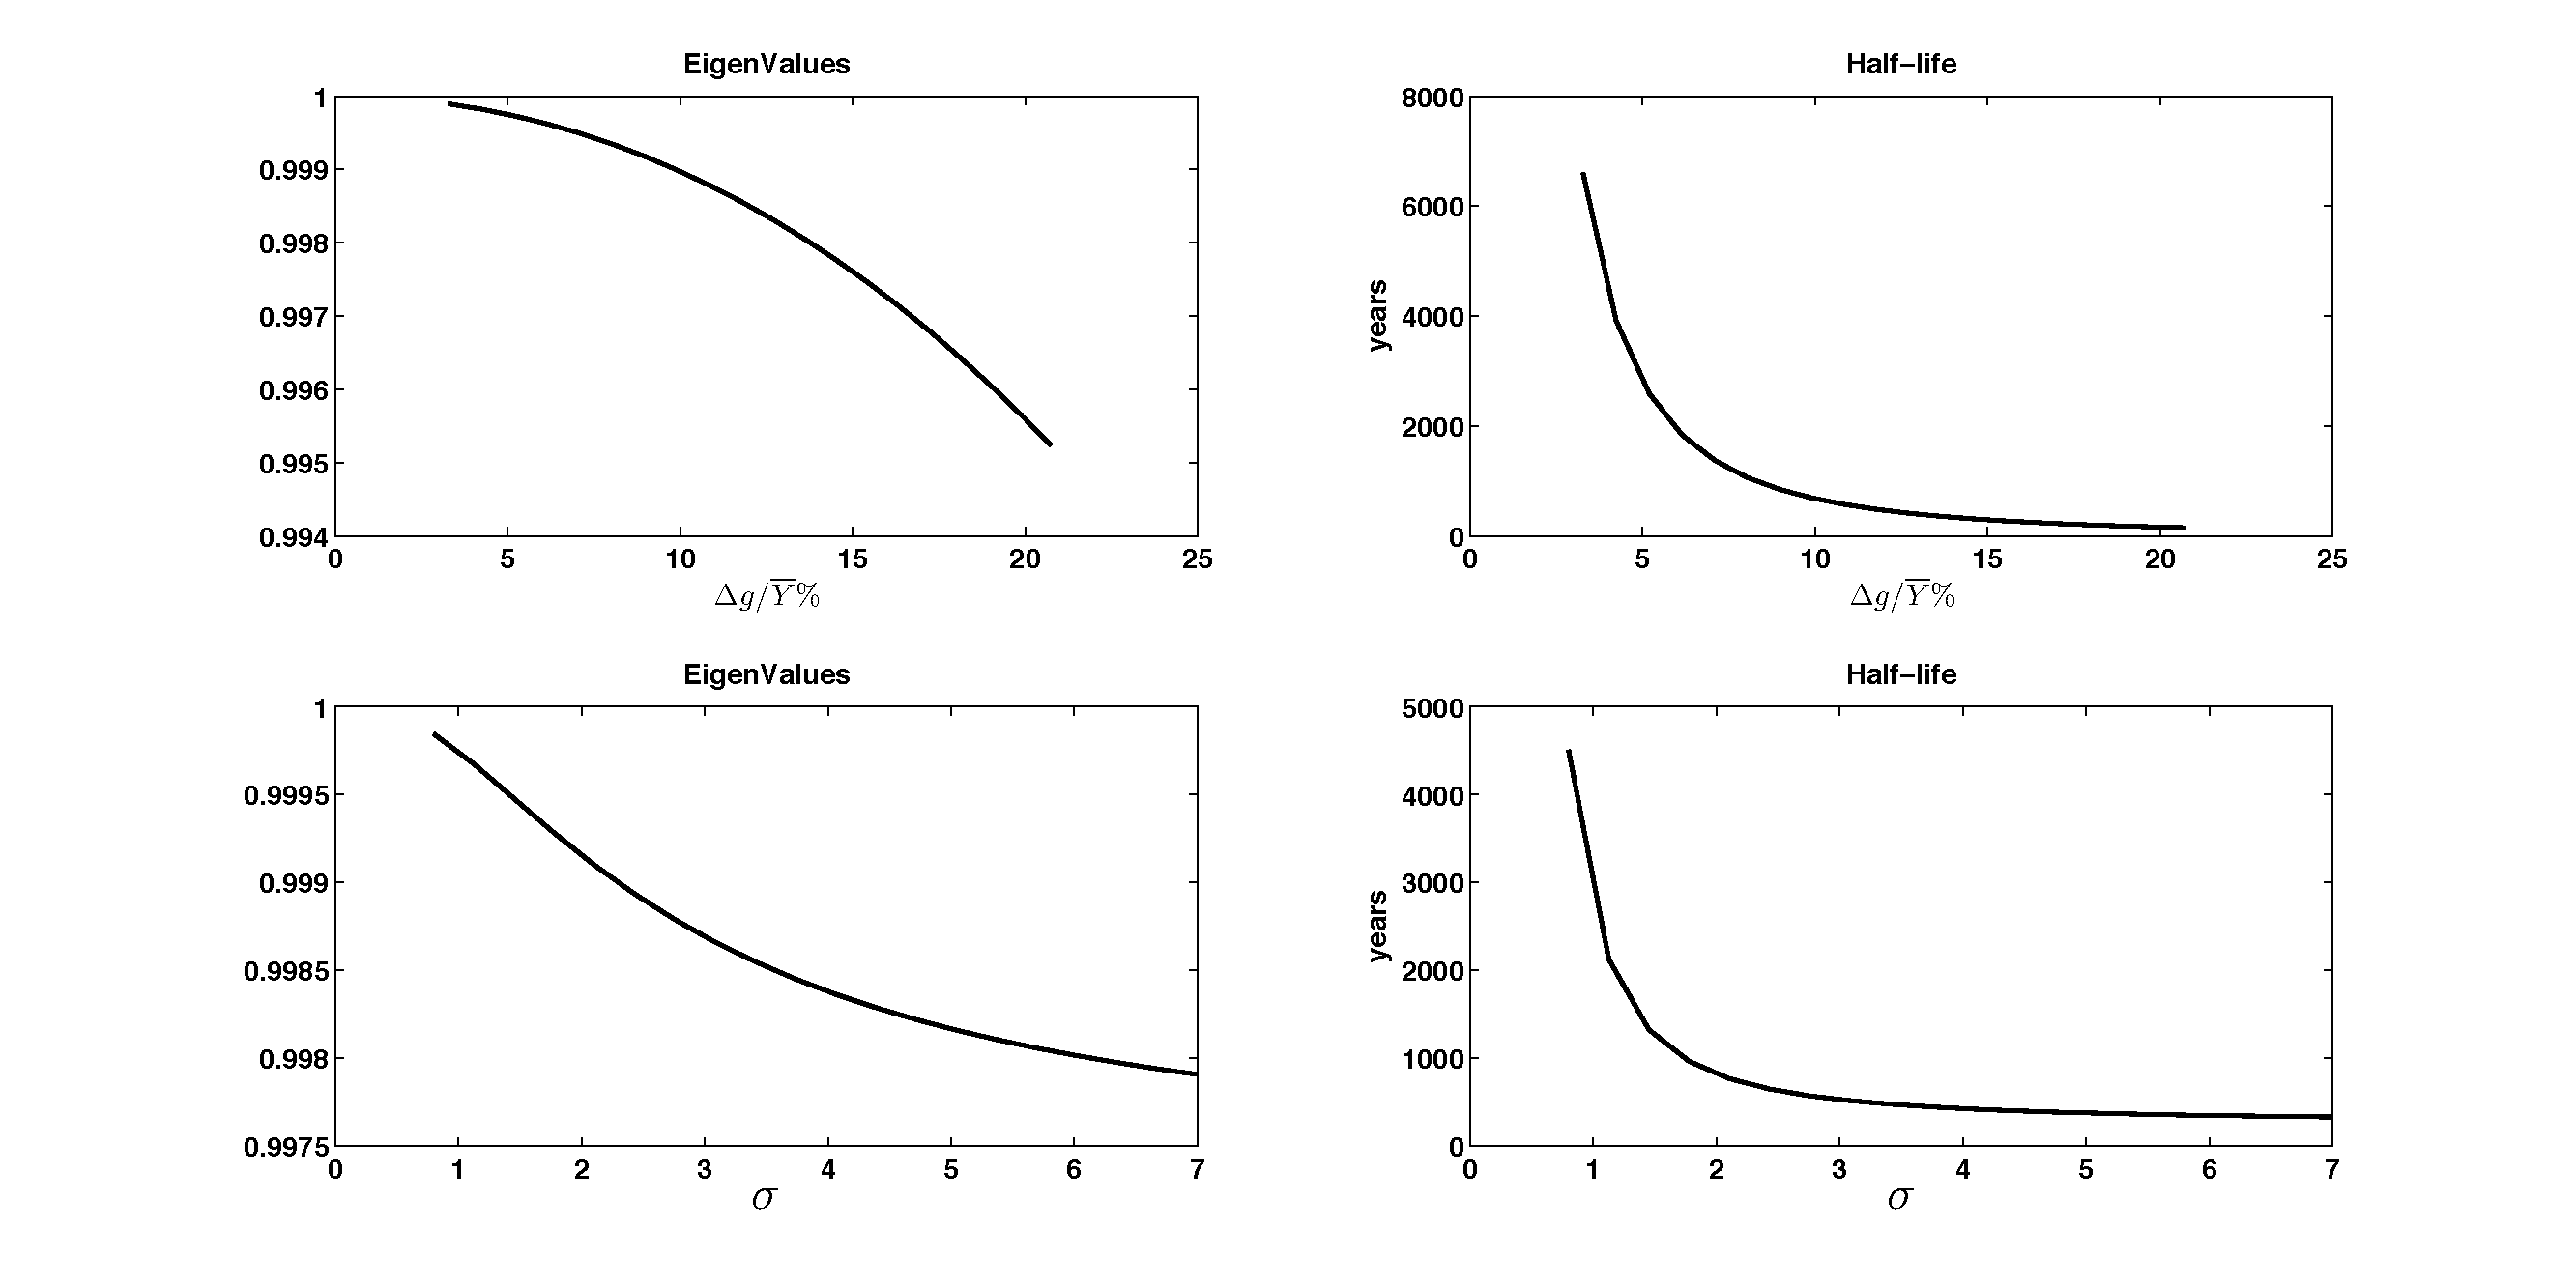
\includegraphics[width=\textwidth]{eigenvalues.pdf}
 \caption{The top (bottom) panel plots the dominant eigenvalue of $\hat{B}$ and the associated half life as we increase
the spread between the expenditure levels (risk aversion). }
 \label{fig: Eigenvalues}
 \end{figure}

\appendix


\bibliographystyle{econ_aer}
\bibliography{BEGS}
\newpage
\end{document}





\subsection{Representative agent}
\label{Sec: rep agent}
This section describes the representative agent environment with risky debt and no transfers. The household values consumption and leisure using a quasilinear utility function and
solves
\begin{equation}
W_0(b_{-1})\max_{\{c_t,l_t,b_{t}\}_t}\mathbb{E}_0\beta^t\left \{c_t-\frac{l_t^{1+\gamma}}{1+\gamma}\right\}
\end{equation}
subject to
\begin{equation}
c_t+b_{t}=(1-\tau_t)\theta l_t+R_tP_tb_{t-t}
\end{equation}
Using the optimality condition for labor and savings we can summarize the set of implementability constraints for the government as follows
\begin{equation}
\label{rep agent QL seq implementability}
b_{t-1} \frac{P_t}{E_{t-1}P_t}=\mathbb{E}_t\sum_{j}\beta^{t+j}[c_{t+j}-l_{t+j}^{1+\gamma}] \quad \forall t
\end{equation}
We also have the feasibility constraint
\begin{equation}
\label{feasibility}
c_t+g_t\leq\theta l_t,
\end{equation}
and the market clearing for bonds $b_t+B_t=0$.





\noindent The optimal Ramsey allocation solves  $\max_{\{c_t,l_t\}_t}W_0(b_{-1})$ subject to \eqref{rep agent QL seq implementability}, feasibility \eqref{feasibility} and natural debt limits for the government $\underline{B}$\footnote{These will be explicitly derived for the examples we solve in this section.}. For the rest of the note we assume i.i.d exogenous shocks to expenditures denote expenditure and payoffs by $g_t=g(s_t)$and $P_t=P(s_t)$ with the normalization $\mathbb{E}P(s)=1$


\begin{theorem}
\label{rep agent general payoffs}

Suppose $P(s)$ satisfies \[P(s)-P(s')>\beta \frac{g(s)-g(s')}{\underline{B}} \quad \forall \quad s,s, \] there exists an invariant distribution of assets with unbounded support. Further for large enough assets (or debt) there is a drift towards the interior region. 

In particular $V$ is strictly concave and there exists $\underline{B}>B_1>B_2>-\infty$ such that

\[\mathbb{E}V'(B(s))>V'(B\_) \quad B\_>B_2 \]
and
\[\mathbb{E}V'(B(s))<V'(B\_) \quad B\_<B_1 \]

\end{theorem}


\begin{theorem}
\label{rep agent policy}
For the two special payoff structures, the optimal tax and asset policies $\{\tau_t,B_t\}_t$ are characterized as follows,
\begin{enumerate}
\item If $P(s)=1$ 
\[\lim_t \tau_t=-\infty, \quad \lim_t B_t=\infty    \quad a.s\]
\item If $P(s) = 1+ \frac{\beta}{ B^*}(g(s) - \mathbb{E} g)$ \quad for some $B^*\geq\underline{B}$
\[\lim_t \tau_t=\tau^*>\infty, \quad \lim_tB_t=  B^*\quad a.s \quad \forall B_{-1} \]

\end{enumerate}
 
\end{theorem}
%When the risky payoff on the bond $P(s)$ perfectly spans $g(s)$,
\begin{remark}
In the case where payoffs are perfectly correlated with expenditure shocks (case 2), we can express the long run assets \[B^*=\beta \frac{\var(g(s))}{\cov(P(s),g(s))}\]. Keeping tax rates (and hence tax revenues in this case) the government needs to finance a higher primary deficit when it gets positive expenditure shock. If in such states the assets pays off more, then optimally the government holds positive assets and uses the these high returns to finance this deficit. On the other hand if payoff are lower in times when the government needs resources, holding debt is valuable since it lowers the interest burden. Thus using the level of its assets $B^*$ it can perfectly span the fluctuations in deficits and the sign is given by the sign of the covariance of $P(s)$ with $g(s)$


The long run tax rate is inversely related to $B^*$ with the following limits,\[\lim_{B^*\to\underline{B}}\tau^*=\frac{\gamma}{1+\gamma}\quad \lim_{B^*\to\infty}\tau^*=-\infty\] 
 
\end{remark}


\begin{corollary}
Let $\underline{B}>-\infty$ be the natural debt limit for the government. Suppose we impose an upper bound on assets $\overline{B}<\infty$,

\begin{enumerate}
\item If $P(s) = 1+ \frac{\beta}{ B^*}(g(s) - \mathbb{E} g)$ \quad for some $\overline{B}>B^*\geq\underline{B}$
\[\exists \epsilon>0, \quad \Pr\{B_t<\underline{B}+\epsilon \text{ or } B_t>\overline{B}-\epsilon\}=0\]

\item For all other payoffs
\[\forall \epsilon>0, \quad \Pr\{B_t<\underline{B}+\epsilon \text{ and } B_t>\overline{B}-\epsilon \}=1\]
\end{enumerate}

\end{corollary}




  

\begin{theorem}
\label{rep agent ergodic distribution}
Consider a orthogonal decomposition of $P(s)$ as follows
\[P(s)=\hat{P}(s)+P^*(s)\] where
\[
  P^*(s) = 1+\frac{\beta}{B^*}( g - \mathbb{E} g) \text{ for some } B^*\geq \underline{B}
\]  
and $\hat{P}(s)$ is orthogonal to $g(s)$. Expanding the policy rules around the steady state of the $P^*(s)$ economy we have the following characterization,

\begin{itemize}
 \item The ergodic distribution of debt of the policy rules linearized around $(B^*, P^*(s))$ will have mean $B^*$, 
 \item The coefficient of variation is given by
  \[
    \frac{\sigma(B)}{\mathbb E(B)} = \sqrt\frac{\var(P(s)) - |\cov(g(s),P(s))|}{(1+|\cov(g(s),P(s))|)|\cov(g(s),P(s))|}\leq\sqrt\frac{\var(P(s)) - |\cov(g(s),P(s))|}{|\cov(g(s),P(s))|}
  \]
  \item The speed of convergence to the ergodic distribution described by
  \[
    \frac{\EE_{t-1}(B_t-B^*)}{(B_{t-1} - B^*)} = \frac1{1+|\cov(P(s),g(s))|}
  \]

\end{itemize}
  

\end{theorem}





\subsection{Heterogeneous agent: Quasilinear unproductive agent}
Suppose the unproductive agent has quasilinear preferences and we additionally impose a non negativity constraint on his consumption.
\begin{theorem}
Let $\omega,n$ be the Pareto weight and mass of the productive agent with $n<\frac{\gamma}{1+\gamma}$. The government trades a risky bond with payoffs $P(s)$ and faces i.i.d expenditure shocks.  The optimal tax, transfer and asset policies $\{\tau_t,T_t,B_t\}$ are characterized as follows,


\begin{enumerate}
 \item For $\omega\geq n \left(\frac{1+\gamma}{\gamma}\right)$ we have  $T_t=0$ and the optimal policy is same as in a representative agent economy studied in theorems \ref{rep agent general payoffs}, \ref{rep agent policy} and \ref{rep agent ergodic distribution}
 \item For $\omega< n \left(\frac{1+\gamma}{\gamma}\right)$, suppose we further assume that $\min_{s}\{P(s)\}>\beta$. We have two parts:
 
 There exists $\mathcal{B}(\omega)$ and $\tau^*(\omega)$ with $\mathcal{B}'(\omega)>0$ and $\lim_{\omega\to 0}\mathcal{B}(\omega)<0$ such that 
 \begin{enumerate}
  \item $B\_>\mathcal{B(\omega)}$
\[T_t>0, \quad \tau_t=\tau^*(\omega), \textit{ and } B_t=B\_ \quad \forall t\] 
\item $B\_\leq \mathcal{B(\omega)}$, the policies depend on the structure of $P(s)$. 
\begin{enumerate}
 \item For a risky bond with $P(s) = 1+ \frac{\beta}{ B^*}(g(s) - \mathbb{E} g)$ \quad for some $B^*<\mathcal{B}(\omega)$ we have two cases depending on $B\_$
\begin{enumerate}
 \item For $B\_\leq B^*$ 
 \[T_t = 0, \quad \lim_t \tau_t=\tau^{**} (\omega), \textit{ and } \lim_tB_t=  B^*\quad a.s \]
\item For $\mathcal{B}(\omega)>B\_>B^*$
\small
\[\Pr\{\lim_t T_t = 0, \lim_t \tau_t=\tau^{**}(\omega),\lim_tB_t=  B^* \textit{ or } \lim_t T_t>0 \text{ i.o.},\lim_t\tau_t=\tau^*(\omega), \lim_tB_t=\mathcal{B}(\omega) \}>0 \]
 \normalsize 
\end{enumerate}

\item For all other payoffs 
   \[\lim_t T_t=0 \text{ i.o.},\quad \lim_t\tau_t=\tau^*(\omega) \text{ and } \lim_tB_t=\mathcal{B}(\omega)\quad \textit{a.s}\]

 \end{enumerate}

 \end{enumerate}

 \end{enumerate}


\end{theorem}




% \begin{theorem}
% \label{main theorem}
% Suppose the Pareto weight of the agents are interior and we normalize the assets of the unproductive agent to zero. 
% Let $n$ and $\omega$ denote the mass and the Pareto weight of the productive agents. The optimal tax, transfer and debt policy $\{\tau_t,T_t,B_t\}_t$ is characterized as follows,
% \begin{enumerate}
% \item As $n\to 0$,
% \[\lim_t T_t=0,\quad \lim_t\tau_t=-\infty \text{ and } \lim_t B_t=\infty\]
% \item As $n\to 1$,
% \[\lim_t T_t=0 \text{ i.o.},\quad \lim_t\tau_t=\frac{-\gamma(\omega-n)}{\omega-(\omega-n)(1+\gamma)} \text{ and } \lim_tB_t=\mathcal{B}(\omega)<\infty\]
% \end{enumerate}
% 
% Furthermore $\mathcal{B}'(\omega)>0$ and $\lim_{\omega\to 0}\mathcal{B}(\omega)<0$
% \end{theorem}
% 
% \begin{corollary}
% Let $\underline{B}>-\infty$ be the natural debt limit for the government. Suppose we impose an upper bound on assets such that, $\mathcal{B}(\omega)<\overline{B}<\infty$. 
% \begin{enumerate}
% \item As $n\to 0$,
% \[\forall \epsilon>0, \quad \Pr\{B_t<\underline{B}+\epsilon \text{ and } B_t>\overline{B}-\epsilon \}=1\]
% \item As $n\to 1$,
% \[\exists \epsilon>0, \quad \Pr\{B_t<\underline{B}+\epsilon \text{ or } B_t>\underline{B}-\epsilon\}=0\]
% \end{enumerate}
% 
% 
% \end{corollary}


\section{Old Discussion}


The purpose of this note is to study the roles of transfers and debt as tools to hedge aggregate shocks in presence of  incomplete markets. 

We begin with the representative agent model studied in AMSS and make two changes:  first, the government trades a ``risky'' bond and second, the government  is prohibited 
from using transfers. The ``risky'' bond is a security whose payoffs $P_t(s^t)$ are correlated with the aggregate shocks. This feature allows us to vary the government's ability to span aggregate shocks while keeping markets incomplete. Below we will characterize two polar cases analytically: a) risk-free bond where $P_t(s^t)=1$ and b) perfect spanning where $\corr(P_t,g_t)=\pm 1$. Lastly we develop an approximation result for intermediate cases.

The main finding is that  the  levels and fluctuations in tax rates and government debt are both
driven by the covariance between  payoff on the bonds and the exogenous  needs for revenue  driven by exogenous government purchases.
With perfect spanning, the joint distribution of  long-run debt and taxes is degenerate, taxes and debt both  diverge in an economy with only
a risk-free bond being traded. The approximation result allows us to estimate the rates of convergence and volatility of debt and taxes for intermediate cases.

The restriction on transfers is meant to capture costs of using this instrument to hedge aggregate shocks. So far these costs are {\em ad hoc}
and assumed to be arbitrarily high. In the next section we endogenize these costs by adding concerns for redistribution and  allowing the government to choose transfers optimally. These concerns are be modeled by adding a positive
mass of unproductive but risk averse agents and assigning to  them a non-zero Pareto weight. Under the assumption that the government trades a risk free bond\footnote{The results for arbitrary payoffs extend analogously, i.e with perfect spanning the government eventually smooths fluctuations in both taxes and transfers.}
we construct two limiting cases of a representative agent economy by varying the mass of either type of agent.

The key insight is that the welfare costs of using fluctuating transfers to hedge aggregate shocks comes from 
the presence (and mass) of the unproductive risk averse agents. As their mass vanishes,
the optimal policy smooths labor taxes and all shocks are hedged by fluctuating transfers. 
In this case, asymptotically transfers diverge and tax rates approach zero. But when the mass of the productive agents is low, 
limiting transfers are constant. Eventually as their mass goes to zero, the optimal policy has unbounded labor subsidies and the level of transfers approaches zero.
In both cases the implied government assets (under the normalization that the unproductive agent holds no assets) diverge.

These limits can be contrasted with an alternative economy in which  the unproductive agents have quasilinear preferences and 
we impose a non-negativity constraint on their consumption. As the mass of these unproductive agents approaches zero, 
limiting taxes are constant (they approach zero if their Pareto weight approaches zero too) but transfers are also zero infinitely often. The government accumulates a  finite level assets (typically positive). Thus the limiting allocation is similar to  that studied in AMSS with a non-negativity constraint on transfers where the government eventually accumulates first best level of assets. However, in our case these levels vary  inversely with the governments' preferences for redistribution and can switch signs for a low enough Pareto weight
on the productive agent. More regressive governments employ
tax subsidies and deficits that are financed by issuing debt. The optimal policy uses transfers as against accumulating assets to hedge aggregate shocks.

\section{Results left on the cutting board}

Besides the results mentioned before we have some things we proved that I could not fit. They mainly pertain to existence of steady state for more general preferences and shocks. I list them in this section


\subsection{Persistence}
\begin{theorem}
Consider a representative agent model studied in section \ref{Sec: rep agent} but with persistence shocks. For every complete market allocation indexed by $\mu^*$ there exists a payoff vector $P(s)$ such that there exists a  steady state in the risky debt economy that supports the same allocation. For an arbitrary payoff vector $P(s)$ (generically) there exists a steady state only if $\|S\|=2$
\end{theorem}


\subsection{Risk Aversion}
We have some scattered results for risk aversion and existence of steady state.
\begin{theorem}
Assume that $U$ is  separable and iso-elastic,	 $U(c,l) = \frac{c^{1-\sigma}}{1-\sigma} -\frac{ l^{1+\gamma}}{1+\gamma}$.
and shocks are i.i.d with $s_b$  being the ``adverse'' state (either low TFP or high govt. expenditures)
and $s_g$ begin the good state. Let $x_{fb}$ be the discounted present value of marginal utility weighted government surpluses associated with the first best allocation.
%\st{ be a value of  %\st{the state $x$ from which a government can implement first=best with complete markets}
%marginal utility weighted debt associated with the first-best allocation with complete markets.}\tjs{David: the phrase
%``first-best allocation with complete markets'' remains imprecise?  What does it mean?}
	 Let $q_{fb}(s)$ be the shadow price of government debt in state $s$ at the first best allocation.
	If
	\begin{equation}\label{eqn:prop52sufficient}
		\frac{1-q_{fb}(s_b)}{1-q_{fb}(s_g)} > \frac{g(s_b)}{g(s_g)}\geq 1 ,
	\end{equation}
		then there exists a steady state with $x_{fb}>x^*>0$
		\end{theorem}



\begin{theorem}
\label{thm long run forces}
Consider an economy consisting of  two types of households with $%
\theta _{1,t}>\theta _{2,t}=0$. One period utilities are $\ln c-\frac{1}{2}%
l^{2}.$ The shock $s$  is i.i.d and takes  two values, $s\in \left\{
s_{L},s_{H}\right\}.$ We assume that $g\left( s\right) =g$ for all $s,$
and $\theta _{1}\left( s_{H}\right) >\theta _{1}\left( s_{L}\right) .$ We allow the discount factor $\beta(s)$ to depend on  $s.$

\smallskip Suppose that $g<\theta (s)$ for all $%
s.$ Let $R(s)$ be the gross interest rates and $x=U^2_c(s)\left[b_2(s)-b_1(s)\right]$

\begin{enumerate}
\item \textbf{Countercyclical interest rates.} If $\beta \left( s_{H}\right) =\beta \left( s_{L}\right)$, then
there exists a steady state $\left( x^{SS},\rho ^{SS}\right) $ such that $%
x^{SS}>0,\ R^{SS}\left( s_{H}\right) <R^{SS}\left( s_{L}\right) .$
\item \textbf{Acyclical interest rates.}  There exists a pair $\left\{ \beta \left( s_{H}\right) ,\beta \left( s_{L}\right)
\right\} $ such that there exists a steady state with $x^{SS}>0$ and $R^{SS}\left(
s_{H}\right) =R^{SS}\left( s_{L}\right)$.
\item \textbf{Procyclical interest rates.} There exists a pair  $\left\{ \beta \left( s_{H}\right) ,\beta \left( s_{L}\right)
\right\} $ such that there exists a steady state with $x^{SS}<0$ and  $R^{SS}\left( s_{H}\right) >R^{SS}\left( s_{L}\right) .$
\end{enumerate}
In all cases, taxes $\tau(s)=\tau^{SS}$ are independent of the realized state.
\end{theorem}

\begin{remark}
 We can extend this result to the case with payoff shocks instead of discount factor shocks
\end{remark}
		
\begin{theorem}
\label{theorem}

Suppose the Pareto weight of the agents are interior and we normalize the assets of the unproductive agent to zero. 
Let $n \in [0,1]$ denote the mass of the productive agents. The optimal tax, transfer and debt policy $\{\tau_t,T_t,B_t\}_t$ is characterized as follows:
\begin{enumerate}
\item As $n\to 0$,
\[\lim_t T_t=0,\quad \lim_t\tau_t=-\infty.\]
\item As $n\to 1$,
\[\lim_t T_t=\infty,\quad \lim_t\tau_t=0.\]
\end{enumerate}
In both cases limiting government assets, $\lim_tB_t=\infty$ 


\end{theorem}
\begin{corollary}
Let $\underline{B}>-\infty$ be the natural debt limit for the government. Suppose we impose an upper bound on assets, $B_t\leq\overline{B}<\infty$
\[\forall \epsilon>0, \quad \Pr\{B_t<\underline{B}+\epsilon \text{ and } B_t>\overline{B}-\epsilon \}=1\]
\end{corollary}

		
		
\begin{theorem}
Consider an economy with at least two agents that are strictly risk averse and a shock process such that there exists a steady state. There do no exists initial conditions i.e a distribution of asset and a choice of Pareto weights such that this allocation can be supported as a complete market Ramsey allocation.
\end{theorem}
		
		

\newpage
\section{Appendix}
\appendix
{\textbf{Theorem 1}}
\begin{proof}




The optimal Ramsey plan solves the following Bellman equation. Let $V(b\_)$ be the maximum ex-ante value the government can achieve with debt $b\_$. 

\begin{equation}
  \label{eq-QLRA obj}
    V(b\_)=\max_{c(s),l(s),b(s)} \sum_{s}\pi(s)\left\{c(s)-\frac{l(s)^{1+\gamma}}{1+\gamma}+\beta V(b(s)) \right\}
\end{equation}   
subject to

   \begin{subequations}
   \label{sys- QLRA constraint}
    \begin{equation}
    \label{rep agent implementability constraint }
    c(s)+b(s)=l(s)^{1+\gamma}+\beta^{-1} P(s)b\_
    \end{equation}
 

 
\begin{equation}
  \label{eq-resoruces}
c(s)+g(s)\leq\theta l(s)
\end{equation}   
Let $\bar{b}=-\underline{B}$
\begin{equation}
  \label{ndl}
b\leq \bar{b}
\end{equation}   


   \end{subequations}
Let $\mu(s)\pi(s),\phi(s)\pi(s)$ be the Lagrange multipliers on the respective constraints. 


\begin{lemma}
There exists  a $\overline{b}$ such that $b_t\leq\overline{b}$. This is the natural debt limit for the government.
\end{lemma}
\begin{proof}
As we drive $\mu$ to $-\infty$, the tax rate approaches a maximum limit, $\bar{\tau}=\frac{\gamma}{1+\gamma}$. In state $s$, the government surplus,
\[
  S(s,\tau) = \theta^\frac\gamma{1+\gamma}(1-\tau)^\frac1\gamma\tau - g(s),
\]  which  is  maximized at $\tau = \frac\gamma{1+\gamma}$ when $(1-\tau)^\frac1\gamma\tau$ is also maximized. This would impose a natural borrowing limit for the government. 

\end{proof}

We begin with some useful lemmas

\smallskip To make this problem convex, let $L\equiv l^{1+\gamma }.$ 

Substitute for $c\left( s\right) $%
\[
V\left( b\_\right) =\max_{L(s),b(s)}\sum_{s\in S}\pi \left(
s\right) \left[ \frac{1}{1+\gamma }L\left( s\right) +\frac{1}{\beta }%
P\left( s\right) b\_-b\left( s\right) +\beta V\left( b\left( s\right)
\right) \right] 
\]%
s.t.%
\begin{eqnarray*}
\frac{1}{\beta }P\left( s\right) b-b\left( s\right) +g\left( s\right) &\leq
&\theta L^{\frac{1}{1+\gamma} }\left( s\right) -L\left( s\right) \\
b\left( s\right) &\leq &\bar{b} \\
L\left( s\right) &\geq &0.
\end{eqnarray*}

\begin{lemma}
\smallskip $V\left( b\right) $ is stictly concave, continuous,
differentiable and $V\left( b\right) <\beta ^{-1}$ for all $%
b<\bar{b}.$ The feasibility constraint binds for all $b\in (-\infty ,\bar{b}%
],\ s\in S$ and $\left( L^{\ast }\left( s\right) \right) ^{1-\frac{1}{1+\gamma} }\geq
\frac{1}{1+\gamma} .\footnote{
This last condition simply means that we do not tax to the right of the peak
of the Laffer curve. The revenue maximizing tax is $1-\bar{\tau}=\frac{1}{%
1+\gamma }.$ At the same time $1-\tau =l^{\gamma}$ so if taxes are always
to the left of the peak, $\frac{1}{1+\gamma }\leq l^{\gamma }=\left(
L^{\frac{1}{1+\gamma} }\right) ^{\gamma}=L^{1-\frac{1}{1+\gamma} }$.}$ 
\end{lemma}

\begin{proof}
\smallskip \textit{Concavity}

$V\left( b\right) $ is concave because we maximize linear objective
function over convex set.

\textit{Binding feasibility}

Suppose that feasibility does not bind for some $b,s.$ Then the optimal $%
L\left( s\right) $ solve $\max_{L\left( s\right) \geq 0}\pi \left( s\right) 
\frac{\gamma}{1+\gamma }L\left( s\right) $ which sets $L\left( s\right)
=\infty .$ This violates feasility for any finite $b,b\left( s\right) .$

\textit{Bounds on }$L$

Let $\phi\left( s\right) >0$ be a Lagrange multiplier on the
feasibility. \ The FOC for $L\left( s\right) $ is 
\[
\frac{1}{1+\gamma }+\phi(s) \left( \frac{1}{1+\gamma }L(s)^{\frac{1}{1+\gamma}
-}-\theta \right) =0. 
\]%
This gives%
\[
\frac{1}{1+\gamma }L^{\frac{1}{1+\gamma} -1}-\theta =-\frac{1}{\lambda }\frac{\gamma}{%
1+\gamma }<0 
\]%
or%
\[
L^{1-\frac{1}{1+\gamma} }\geq \frac{\theta }{1+\gamma }. 
\]

\textit{Continuity}

For any $L$ that satisfy $L^{1-\frac{}{1+\gamma} }\geq \frac{\theta }{1+\gamma} ,$ define function $%
\Psi $ that satisfies $\Psi \left( L^{\frac{1}{1+\gamma} }-\theta L\right) =L.$ Since $%
L^{\frac{1}{1+\gamma} }-L$ is strictly decreasing in $L$ for $L^{1-\frac{1}{1+\gamma} }\geq
\frac{1}{1+\gamma} $, this function is well defined. Note that $\Psi \left(
{}\right) \underbrace{\left( \frac{1}{1+\gamma }L^{\frac{1}{1+\gamma} -1}-\theta \right) }%
_{<0}=1$ (so that $\Psi >0$, i.e. $\Psi $ is strictly decreasing)
and $\Psi ^{\prime \prime }\underbrace{\left( \frac{1}{1+\gamma }L^{\frac{1}{1+\gamma}
-1}-1\right) ^{2}}_{>0}+\underbrace{\Psi }_{<0}\underbrace{\frac{1%
}{1+\gamma }\frac{\gamma }{1+\gamma }L^{\frac{1}{1+\gamma} -2}}_{<0}=0$ (so that $\Psi
^{\prime \prime }\geq 0$, $\Psi ^{\prime \prime }>0,$ i.e. $\Psi $ is
strictly concave on the interior). $\Psi $ is also continuous. When $%
L^{1-\frac{1}{1+\gamma} }=\frac{1}{1+\gamma} ,$ $L=(1+\gamma) ^{-\frac{(1+\gamma)} {\left( \gamma \right)} }.$
Let $D\equiv (1+\gamma) ^{\frac{-1}{ \gamma }-(1+\gamma) ^{-\frac{1+\gamma }{\left(\gamma\right)} }}.$ Then the objective is 
\[
V\left( b\_\right) =\max_{b\left( s\right) }\sum_{s\in S}\pi \left(
s\right) \left[ \Psi \left( \frac{1}{\beta }P\left( s\right) b-b\left(
s\right) +g\left( s\right) \right) +\frac{1}{\beta }P\left( s\right)
b\_-b\left( s\right) +\beta V\left( b\left( s\right) \right) \right] 
\]%
s.t.%
\begin{eqnarray*}
b\left( s\right) &\leq &\bar{b} \\
\frac{1}{\beta }P\left( s\right) b\_-b\left( s\right) +g\left( s\right) &\leq
&D.
\end{eqnarray*}

This function is continuous so $V$ is also continuous.

\textit{Differentiability}

Continuity and convexity implies differentiability everywhere, including the
boundaries.

\textit{Strict concavity}

$\Psi $ is strictly concave, so on the interior $V$ is strictly
concave.

\end{proof}


\begin{lemma}
With $P(s)=1$, the multiplier on the implementability constraint,$\lim_t\mu_t=\mu*$
\end{lemma}
\begin{proof}
 

The envelope theorem together with the FOC with respect to $b(s)$ imply that the multiplier on the implementability constraint is a martingale

\[\mathbb{E}\mu_{t+1}=\mu_t\]

The FOC with respect to labor $l(s)$ can be expressed as 

\[\mu=\frac{\frac{\theta}{l^{\gamma}-1}}{\frac{\theta}{l^{\gamma}-(1+\gamma)}}\]. Note that $(1-\tau)^{-1}=\theta/l^{\gamma}$. Thus, as tax rates go to $-\infty$, $\mu$ approaches $\frac{1}{1+\gamma}$ from below.

Given this bound, the standard martingale convergence theorems imply that $\mu\to \mu^*$ almost surely. 
\end{proof}



We first show that  if $\mu^*=\frac{1}{1+\gamma}$, $b_t\to-\infty$ and then argue that $\mu^*$ cannot converge to any other value. 



Strict concavity of $V$ implies $\mu$ converges, either $b_t$ converges to a constant or diverges to $-\infty$. Suppose $\lim_tb_t$ is finite. The government's budget constraint would imply

\begin{equation}
\label{gbc}
\lim_t \tau_t\theta l_t-\lim_tg_t=(\beta^{-1}-1)\lim_t b_t
\end{equation}



However the left hand side of the previous expression diverges to $-\infty$. However under the hypothesis the right hand side is finite. This gives us a contradiction and hence $\lim_tb_t=-	\infty$. 

Now suppose $\mu^*<\frac{1}{1+\gamma}$. Again strict concavity of $V$ implies $\lim_t b^*>-\infty$.  However, labor supply and taxes will be constant and finite in the limit. Thus, the left hand side of \eqref{gbc} is stochastic and the right hand side approaches a constant. This yields a contradiction.


Thus, combining the above, $\mu^*=\frac{1}{1+\gamma}$ and $\lim_tb_t=-\infty$.







The second part of the theorem is to prove convergence to $B^*$ for a the class of payoffs that are perfectly aligned with the expenditure shocks. We first begin with some characterization of the policy rules
\smallskip Next we characterize policy functions

\begin{lemma}
\label{lem increasing b}
$b\left( b\_,s\right) $ is an increasing function of $b$ for all $s$ for all $%
\left( b\_,s\right) $ where $b\left( s\right) $ is interior.
\end{lemma}

\begin{proof}
Take the FOCs for $b\left( s\right) $ from the condition in the previous
problem. If $b\left( s\right) $ is interior%
\[
\Psi \left( \frac{1}{\beta }P\left( s\right) b\_-b\left( s\right)
+g\left( s\right) \right) =\beta V\left( b\left( s\right)
\right) . 
\]

Suppose $b_{1}<b_{2}$ but $b_{2}\left( s\right) <b_{1}\left( s\right) .$
Then from stict concavity%
\begin{eqnarray*}
V\left( b_{2}\left( s\right) \right) &<&V^{\prime
}\left( b_{1}\left( s\right) \right) \\
\Psi \left( \frac{1}{\beta }P\left( s\right) b_{2}-b_{2}\left(
s\right) +g\left( s\right) \right) &>&\Psi \left( \frac{1}{\beta }%
P\left( s\right) b_{1}-b_{1}\left( s\right) +g\left( s\right) \right) .
\end{eqnarray*}
\end{proof}



\begin{lemma}  Let $\mu(b,s)$ be the optimal policy function for the Lagrange multiplier $\mu(s)$.  If $P(s') > P(s'')$ then there exists a $b^*_{s',s''}$ such that for all $b < (>) \; b_{1,s',s''}$ we have $\mu(b,s') > (<) \;\mu(b,s'')$.  If $\underline b < b^*_{s',s''} < \overline b$ then $\mu(b^*_{s',s''},s') = \mu(b^*_{s',s''},s'')$.
\label{lem.order}
\end{lemma}
\begin{proof} 
Suppose that $\mu(b,s')\leq \mu(b,s'')$.  Subtracting the implementability for $s''$ from the implementability constraint for $s'$ we have 
\begin{align*}
	\frac{P(s')-P(s'')}{\beta}b &= S_{s'}(\mu(b,s'))-S_{s''}(\mu(b,s'')) + b'(b,s')-b'(b,s'')\\
						&\geq S_{s'}(\mu(b,s')) -S_{s''}(\mu(b,s')) + b'(b,s')-b'(b,s'')\\
						&\geq  S_{s'}(\mu(b,s')) -S_{s''}(\mu(b,s')) = g(s'')-g(s')
\end{align*}  We get the first inequality from noting that $S_s(\mu')\geq S_s(\mu'')$ if $\mu' \leq \mu''$.  We obtain the second inequality by noting that $\mu(b,s')\leq \mu(b,s'')$ implies $b'(b,s')\geq b'(b,s'')$ (which comes directly from the concavity of $V$).
Thus, $\mu(b,s')\leq \mu(b,s'')$ implies that 
\[
	b \geq \frac{\beta(g(s'')-g(s'))}{P(s')-P(s'')} = b^*_{s',s''}
\]The converse of this statement is that if $b<b^*_{s',s''}$ then $\mu(b,s') > \mu(b,s'')$.  The reverse statement that $\mu(b,s') \geq \mu(b,s'')$ implies $b \leq b^*_{s,s'}$ follows by symmetry.   Again, the converse implies that if $b > b^*_{s',s''}$ then $\mu(b,s') < \mu(b,s'')$.    Finally, if $\underline b < b^*_{s',s''} <\overline b$ then continuity of the policy functions implies that there must exist a root of $\mu(b,s')-\mu(b,s'')$ and that root can only be at $b^*_{s',s''}$.
\end{proof}

The FOC and the envelope theorem now modify the martingale equation for $\mu_t$ as follows,
\begin{equation}
\label{eq.mart}
\sum_{s}\pi(s)P(s)\mu(s)=\mu\_
\end{equation}

With Lemma \ref{lem.order} we can order the policy functions $\mu(b,\cdot)$ for particular regions of the state space.  Take $b_1$ to be
\[
	b_1 = \min\left\{b^*_{s',s''}\right\}
\] and WLOG choose $\underline b < b_1$.  For all $b < b_1$ we have shown that $P_s > P(s')$ implies that $\mu(b,s) > \mu(b,s')$.  By decomposing $\EE \mu_{t+1}P_{t+1}$ in equation \eqref{eq.mart}, we obtain (using $\EE_t P_{t+1} = 1$)
\begin{equation}
	\mu_t = \EE\mu_{t+1} +\cov_t(\mu_{t+1},P_{t+1})
\end{equation}Our analysis has just shown that for $b_t < b_1$ we have $\cov_t (\mu_{t+1},P_{t+1})  >0$ so 
\[
	\mu_t > \EE_t\mu_{t+1}.
\]  If $p$ is sufficiently volatile:
\[
	P(s') - P(s'') > \frac{\beta(g(s'')-g(s'))}{\overline b}
\] then 
\[
	b_2 = \max\left\{b^*_{s',s''}\right\} <\overline b
\] and through a similar argument  we can conclude that $\cov_t(\mu_{t+1},P_{t+1}) < 0$ 
\[
	\mu_t < \EE_t \mu_{t+1}
\] for $b_t > b_2$


\begin{lemma}
For payoff structures of the form
if \[
  P(s) = 1 + \alpha(g(s)- \EE g)\]
 then  there exists a unique $b^*$ such that $b(b^*,s)=b^*$ for all $s$  
\end{lemma}
\begin{proof}
This follows from taking differences of the \eqref{rep agent implementability constraint } for $s'$,$s''$. We have 
\[[P(s)-P(s'')]\frac{b^*}{\beta}=g(s)-g(s'')\]
We have used the fact that if $b(b^*,s)$ is invariant across states, $\mu(s)=\mu^*$ and this implies that tax rates are constant. Thus, the fluctuations in the surplus of the government only come from $g(s)$.

\end{proof}

Since are payoffs $P(s)$ in this second part are linear in $g(s)$, we can immediately see that by setting $\alpha=\frac{\beta}{b^*}$
 


\begin{lemma}
\label{sub super martingale}
$\mu_t$  is a sub-martingale bounded above in the region $(-\infty,\mu^*)$ and super-martingale bounded below in the region $(\mu^*,\frac{1}{1+\gamma})$


\end{lemma}
\begin{proof}
Let $\mu^*$ be the associated multiplier, i.e $V_b(b^*)=\mu^*$.  Using the results of the previous section, we have that $b_1 = b_2 = b^*$, implying that $\mu_t < (>) \EE_t\mu_{t+1}$ for $b_t  < (>) b^*$. 
\end{proof}

Lastly we show that $\lim_t \mu_t=\mu^*$. Suppose $b_{t}<b^*$, we know that $\mu_t>\mu^*$. The previous lemma implies that in this region, $\mu_t$ is a super martingale. The lemma $\ref{lem increasing b}$ shows that $b(b\_,s)$ is continuous and increasing. This translates into $\mu(\mu(b\_),s)$ to be continuous and increasing as well.
 Thus 
 \[\mu_{t}>\mu^* \implies \mu(\mu_{t},s_{t+1})>\mu(\mu^*,s_{t+1}) \]
or
 \[\mu_{t+1}>\mu^*\]
Thus $\mu*$  provides a lower bound to this super martingale. Using standard martingale convergence theorem converges. The uniqueness of steady state implies that it can only converge to $\mu^*$. For $\mu<\mu^*$, the argument is symmetric.



\end{proof}

{\textbf{Corollary 1}}


\begin{proof}
Here we show that for $P(s)=1$ we show that with probability one, $b_t$ gets arbitrary close to both the boundaries. Adding a lower bound to debt imposes a constraint
\begin{equation}
\label{bound on b}
b(s)\geq\underline{b}
\end{equation}
The foc with respect to $b(s)$ will now be modified to

\[\beta \pi(s) V'(b(s))+\pi(s)\kappa(s)=\mu(s)\]
where $\kappa(s)$ is the Lagrange multiplier on the \eqref{bound on b}.  We first show a lemma that allows us to strictly order $b(b\_,s)$ across $s$

\begin{lemma}
\label{prop: b(s) relative to b}For any $b\_\in (-\underline{b} ,\bar{b}),$ there are $s,s^{\prime \prime }$ s.t. $b\left( s\right) \geq b\_\geq b\left( s^{\prime \prime }\right) .$ Moreover, if there are any states $s^{\prime \prime },s^{\prime \prime \prime }$ s.t. $b\left( s^{\prime \prime
}\right) \neq b\left( s^{\prime \prime \prime }\right) ,$ those inequalities
are strict.
\end{lemma}


\begin{proof}
The FOCs together with the envelope theorem imply that $\mathbb{E}P(s)V'(b(s))=V'(b\_)+\kappa(s)$
We can rewrite this as $\mathbb{\tilde{E}}V'(b(s))=b+\kappa(s)$ with $\tilde{\pi}(s)=P(s)\pi(s)$

Now if there is at least one $b\left( s\right) $ s.t. $b\left(
s\right) >b\_,$ by strict concavity of $V$ there must be some $%
s^{\prime \prime }$ s.t. $b\left( s^{\prime \prime }\right) <b.$

If there is at least one $b\left( s\right) $ s.t. $b\left(
s\right) <b\_,$ the inequality above is strictly only if $b\left(
s^{\prime \prime \prime }\right) =\bar{b}$ for some $s^{\prime \prime \prime
}.$ But $V\left( \bar{b}\right) <V\left(
b\right) $ so there must be some $s^{\prime \prime }$ s.t. $b\left(
s^{\prime \prime }\right) >b.$ Equality is possible only if $b\_=b\left(
s\right) $ for all $s.$
\end{proof}

For payoffs $P(s)=1$, it is easy to see that there does not exists any $b^*$ in the interior that has the property $b(b^*,s)=b^*$. Thus, the relevant inequalities in the previous lemma are strict. This allows us to construct a sequences $\{b_t\}_t $ such that $b_t<b_{t+1}$ with the property that $\lim_tb_t=\underline{b}$.
Thus, for any $\epsilon>0$, there exists a finite history of shocks that can take us arbitrarily close to $\underline{b}$. Since the shocks are i.i.d this finite sequence will repeat i.o. With a symmetric argument we can show that $b_t$ will come arbitrarily close to its upper limit i.o too




The second part of the corollary states that $P(s)=1+\frac{\beta}{B^*}(g(s)-\mathbb{E}g)$ then we never approach the boundaries. This essentially follows from lemma \ref{sub super martingale}. We have the covariance $\cov(\mu_{t+1},P(s_{t+1})<0$ for $\mu<\mu^*$ and vice versa. The only change is that the martingale equation for $\mu$ will read
\[\mathbb{E}\mu_{t+1}=\mu_t-\cov(\mu_{t+1},P(s_{t+1})-\kappa_{t+1}\]

Note that for $\mu<\mu^*$ $\kappa_{t+1}$ will be zero and the analysis is same as before. For $\mu>\mu^*$ we have the covariance term positive and the Lagrange multiplier positive too. Thus
\[\mathbb{E}\mu_{t+1}<\mu_t\]
Thus, it remains a super-martingale drifting towards $\mu^*$.
\end{proof}



{\textbf{Theorem 2}}
\begin{proof}
The first order conditions for a planning problem given portfolio $p_s$ are given by
\begin{align*}
	\frac{b p_s}{\beta \EE p}= S(\mu'(s),s) + b'(s)\\
	V'(b) = \frac{\EE p \mu'}{\EE p}\\
	\mu'(s) = V'(b'(s))
\end{align*} where $S(\mu,s)$ is the government surplus in state $s$ given by
\[
	S(\mu,s) = (1-\tau(\mu))^\frac1\gamma \tau(\mu)-g(s) = I(\mu) - g(s)
\]where
\[
	\tau(\mu) =\frac{\gamma\mu}{(1+\gamma)\mu-1}
\]We note that $V'(b)$ is one-to-one, so we can re-characterize these equations as searching for a function $b(\mu)$ such that the following two equations can be solved for all $\mu$.
\begin{align}\label{eq.lin_imp}
	\frac{b(\mu)p_s}{\beta \EE p} = I(\mu'(s)) - g(s) +b(\mu'(s))\\
	\mu = \frac{\EE\mu' p}{\EE p}\label{eq.lin_mart}
\end{align}  This defines, implicitly, a function $b(\mu; p)$ .  For a given $\overline \mu$ define 
\[
	\overline b = \frac{\beta}{1-\beta}\left( I(\overline\mu) - \overline g\right)
\]where $\overline g = \EE g$ and $\overline p$ as 
\[
	\overline p_s = 1+ \frac\beta{\overline b}(g_s - \overline g)
\]  As noted before $b(\overline\mu;\overline p) = \overline b$ solves the the system of equations (\ref{eq.lin_imp}-\ref{eq.lin_mart}) for $\mu'(s) = \overline \mu$.  We can linearize around this steady state with respect to both $\mu$ and $p$.  Differentiating equation \eqref{eq.lin_imp} with respect to $\mu$ around $(\overline \mu,\overline p)$ we obtain
\[
	\frac{\pbar_s}{\beta}\frac{\partial b}{\partial \mu} = \left[I'(\mubar)+\frac{\partial b}{\partial \mu}\right]\frac{\partial \mu'(s)}{\partial \mu}.
\]Differentiating equation \eqref{eq.lin_mart} with respect to $\mu$ we obtain
\[
	1 = \sum_{s'} \Pi_s \overline p_s \frac{\partial \mu'(s)}{\partial \mu}
\]combining these two equations we see that 
\[
	\frac1\beta\left(\sum_s\Pi_s\pbar_s^2\right)\frac{\partial b}{\partial \mu} = I'(\mubar) + \frac{\partial b}{\partial \mu}
\]Noting that $\EE\overline p^2 = 1 + \frac{\beta^2}{\bbar^2}\sigma^2_g$ we obtain
\begin{equation}
	\frac{\partial b}{\partial \mu} = \frac{I'(\mubar)}{\frac{\beta}{\bbar^2}\sigma_g^2 +\frac{1-\beta}{\beta}} < 0
\end{equation}as $I'(\mubar) < 0$.  We then have directly that 
\begin{equation}
	\frac{\partial \mu'(s)}{\partial \mu} = \frac{\overline p_s}{\frac{\beta^2}{\overline b^2}\sigma^2_g +1} = \frac{\pbar_s}{\EE\pbar^2}
\end{equation}  We can perform the same procedure for $p_s$.  Differentiating equation \eqref{eq.lin_imp} with respect to $p_s$ we around $(\mubar,\pbar)$ we obtain
\begin{equation}\label{eq.dimp_dps}
\frac{\pbar_{s'}}{\beta}\frac{\partial b}{\partial p_s} + 1_{s,s'}\frac{\bbar}{\beta} - \frac{\Pi_s\bbar\pbar_{s'}}{\beta} = \left[I'(\mubar) + \frac{\partial b}{\partial \mu}\right]\frac{\partial \mu'(s')}{\partial p_s}
\end{equation} Here $1_{s,s'}$ is $1$ if $s = s'$ and zero otherwise.  Differentiating equation \eqref{eq.lin_mart} with respect to $p_s$ we obtain
\[
	0 = \Pi_s\mubar - \Pi_s\mubar + \sum_{s'} \Pi_{s'}\pbar_s\frac{\partial \mu'(s')}{\partial p_s} =  \sum_{s'} \Pi_{s'}\pbar_s\frac{\partial \mu'(s')}{\partial p_s}
\]  Again we can combine these two equations to give us
\[
	\frac{\EE\pbar^2}{\beta}\frac{\partial b}{\partial p_s} + \frac{\Pi_s\bbar}{\beta}(\pbar_s-\EE\pbar^2) = 0
\] or
\begin{equation}
	\frac{\partial b}{\partial p_s} = \Pi_s\bbar \frac{\EE\pbar^2-\pbar_s}{\EE\pbar^2}
\end{equation}Going back to equation \eqref{eq.dimp_dps} we have
\begin{equation}
	\frac{\partial \mu'(s')}{\partial p_s} = \frac{\bbar}{\beta\left[I '(\mubar) + \frac{\partial b}{\partial \mu}\right]}\left(1_{s,s'}-\frac{\Pi_s\pbar_s\pbar_{s'}}{\EE\pbar^2}\right)
\end{equation}
\subsection{Ergodic Distribution of the Linearized System}
The linearized system for $\mu$ now follows
\[
	\hat \mu_{t+1} = B \hat\mu_t + C
\]  where $B$ and $C$ are both random with means $\barB$ and $\barC$, and variances $\sigma_B^2$ and $\sigma_C^2$ .  Suppose that $\hat\mu$ is distributed according to the ergodic distribution of this linear system with mean $\EE\hat\mu$ and variance $\sigma^2_\mu$.  Since 
\[
	B\hat\mu +C
\]has the same distribution we can compute the mean of this distribution as
\[
\begin{split}
	\EE\hat\mu &= \EE\left[ B\hat\mu+C\right]\\
			  &= \EE\left[\EE_{\hat\mu}\left[B\hat\mu+C\right]\right]\\
			  &= \EE\left[\barB\hat\mu +\barC\right]\\
			  &=\barB\EE\hat\mu+\barC
\end{split}
\]solving for $\EE\hat\mu$ we get
\begin{equation}
	\EE\hat\mu = \frac{\barC}{1-\barB}
\end{equation}For the variance $\sigma^2_{\hat\mu}$ we know that 
\[
	\sigma^2_{\hat\mu} = \var(B\hat\mu+C) = \var(B\hat\mu) + \sigma_C^2 + 2\cov(B\hat\mu,C)
\]Computing the variance of $B\hat \mu$ we have
\[
\begin{split}
	\var(B\hat\mu) &=\EE\left[(B\hat\mu - \barB\EE\hat\mu)^2\right]\\
			       &=\EE\left[(B\hat\mu-\barB\hat\mu +\barB\hat\mu -\barB\EE\hat\mu)^2\right]\\
			      &=\EE\left[\EE_{\hat\mu}\left[(B-\barB)^2\hat\mu^2 +2(B-\barB)(\hat\mu-\EE\hat\mu)\barB\EE\hat\mu + (\hat\mu-\EE\hat\mu)^2\bar B^2\right]\right]\\
			&=\EE\left[\sigma_B^2\hat\mu^2 +(\hat\mu-\EE\hat\mu)^2\barB\right]\\
			& = \sigma_B^2(\sigma_{\hat\mu}^2+(\EE\hat\mu)^2) + \sigma_{\hat\mu}^2\barB^2
\end{split}
\]while for the covariance of $B\hat\mu$ and $C$
\[
	\cov(B\hat\mu,C) = \sigma_{BC}\EE\hat\mu
\]Putting this all together we have
\begin{equation}
	\sigma_{\hat\mu}^2 = \frac{\sigma_B^2(\EE\hat\mu)^2 + \sigma_{BC}\EE\hat\mu + \sigma_C^2}{1-\barB^2-\sigma_B^2}
\end{equation}
\subsection{What is the best $\pbar$}
We want to study the properties of the ergodic distribution of an economy with payoff structure $ p_s$, normalized so that $\EE p = 1$.  The immediate question to ask is where we should linearize around?  The natural answer is to choose $\mubar$ so as to minimize 
\[
\| p-\pbar(\mubar)\|^2 = \sum_{s'}\Pi_{s'}( p_{s'}-\pbar(\mubar)_{s'})^2.
\]That is to choose $\mubar$ so as to minimize the variance of the difference between $ p$ and the set of steady state payoffs.  We shall see how this is the ``best'' choice by another metric.  The first order condition for this linearization gives us 
\[
	2\sum_{s'}\Pi_s'( p_{s'}-\pbar(\mubar)_{s'}) \pbar'(\mubar)_{s'} = 0
\]as noted before 
\[
	\pbar(\mubar)_s =  1 -\frac{\beta}{\bbar(\mubar)}\left(g_s - \EE g\right)
\]thus
\[
	\pbar'(\mubar) \propto \pbar(\mubar)-1
\]Thus, we can see the the optimal choice of $\mubar$ is equivalent to choosing $\mubar$ such that 
\begin{equation}
	\begin{split}
		0 &= \sum_{s'}\Pi_{s'}( p_{s'} - \pbar(\mubar)_{s'})(\pbar(\mubar)_{s'}-1)\\
		&= -\sum_{s'}\Pi_{s'}( p_{s'}-\pbar(\mubar)_{s'}) + \sum_{s'}\Pi_{s'}( p_{s'}-\pbar(\mubar)_{s'})\pbar(\mubar)_{s'}\\
		&= \sum_{s'}\Pi_{s'}( p_{s'}-\pbar(\mubar)_{s'})\pbar(\mubar)_{s'}\\
		&=\EE\left[( p-\pbar(\mubar))\pbar(\mubar)\right]
	\end{split}
\end{equation}  Using this $\pbar$ and $\mubar$ we have that $C$ for our linearized system is
\[
	C_{s'} = \sum_s\left\{\frac{\bbar}{\beta\left[I'(\mubar)+\frac{\partial b}{\partial\mu}\right]}\left(1_{s,s'}-\frac{\Pi_s \pbar_s\pbar_{s'}}{\EE\pbar^2}\right)({p}_s-\pbar_s) \right\}
\]Taking expectations we have that 
\begin{equation}
\begin{split}
	\barC &= \sum_s\left\{\frac{\bbar}{\beta\left[I'(\mubar)+\frac{\partial b}{\partial\mu}\right]}\left(\Pi_s - \frac{\Pi_s\pbar_s}{\EE\pbar^2}\right)( p_s-\pbar_s)\right\}\\
	&=\frac{\bbar}{\beta\left[I'(\mubar)+\frac{\partial b}{\partial\mu}\right]}\left(\EE( p-\pbar) -\frac{\EE\left[( p-\pbar)\pbar\right]}{\EE\pbar^2}\right)\\
	&= 0 
\end{split}
\end{equation}  Thus, the linearized system will have the same mean for $\mu$, $\mubar$, as the closest approximating steady state payoff structure.

We can also compute the variance of the ergodic distribution for $\mu$.  Note 
\[
\begin{split}
	C_{s'} &= \sum_s\left\{\frac{\bbar}{\beta\left[I'(\mubar)+\frac{\partial b}{\partial\mu}\right]}\left(1_{s,s'}-\frac{\Pi_s \pbar_s\pbar_{s'}}{\EE\pbar^2}\right)({p}_s-\pbar_s) \right\}\\
		 &=\frac{\bbar}{\beta\left[I'(\mubar)+\frac{\partial b}{\partial\mu}\right]}\left( p_{s'}-\pbar_{s'} -\pbar_{s'}\frac{\sum_s\Pi_s\pbar_s( p_s-\pbar_s)}{\EE\pbar^2}\right)\\
		&= \frac{\bbar}{\beta\left[I'(\mubar)+\frac{\partial b}{\partial\mu}\right]}( p_{s'}-\pbar_{s})
\end{split}
\]  As noted before
\[
	\sigma_{\mu}^2 = \frac{\bbar^2}{\beta^2\left[I'(\mubar)+\frac{\partial b}{\partial\mu}\right]^2\left(1-\barB^2-\sigma_B^2\right)}\| p-\pbar\|^2
\]  The variance of government debt in the linearized system is 
\[
	\sigma_b^2 = \frac{\bbar^2\left(\frac{\partial b}{\partial\mu}\right)^2}{\beta^2\left[I'(\mubar)+\frac{\partial b}{\partial\mu}\right]^2\left(1-\barB^2-\sigma_B^2\right)}\| p-\pbar\|^2
\]  This can be simplified using the following expressions: 
\[
	I'(\mubar)+\frac{\partial b}{\partial \mu} = \frac{\EE\pbar^2}{\beta}\frac{\partial b}{\partial\mu},
\]
\[
	\barB = \frac{1}{\EE\pbar^2}
\]and
\[
	\sigma_B^2 = \frac{\var(\pbar)}{(\EE\pbar^2)^2}
\] to
\begin{equation}
	\sigma^2_b = \frac{\bbar^2}{\EE\pbar^2\var(\pbar)}\|p-\pbar\|^2
\end{equation}Noting that $\EE\pbar^2 = 1 +\var(\pbar) > 1$, we have immediately that up to first order the relative spread of debt is bounded by
\begin{equation}
	\frac{\sigma_b}{\bbar} \leq \sqrt\frac{\|p-\pbar\|^2}{\var(\pbar)}
\end{equation}  Thus, as $p$ approaches a the steady state payoff vector the ergodic distribution becomes degenerate.
\end{proof}


{\textbf{Theorem 3}}

\begin{proof}

Suppose the unproductive agent has CRRA utility function with risk aversion $\sigma$. Under these assumption we can formulate the Bellman equation that solves for the Ramsey plan as follows:


\begin{equation}
  \label{eq-QLRA obj}
    V(b\_,\rho\_)=\max_{c_1(s),c_2(s),\rho(s), b(s)} \sum_{s}\pi(s)\left\{\omega \left[u(c_1(s),l_1(s))\right]+(1-\omega )\left[\frac{c_2(s)^{1-\sigma}}{1-\sigma}\right]+\beta V(b(s),\rho(s)) \right\}
\end{equation}   
subject to

   \begin{subequations}
   \label{sys- QLRA constraint}
    \begin{equation}
    \label{eq-implementability constraint}
    c_1(s)-c_2(s)+b(s)=l(s)^{1+\gamma}+\beta^{-1} b\_
    \end{equation}
 
\begin{equation}
   \label{eq-ee}
\mathbb{E}c_2^{-\sigma}(s)=\rho\_
\end{equation}   

\begin{equation}
   \label{eq-definition rho}
   \rho(s)=c_2^{-\sigma}(s)
\end{equation}   

 
\begin{equation}
  \label{eq-resoruces}
    n c_1(s)+(1-n)c_2(s)+g(s)\leq\theta_2 n l(s)
\end{equation}   


   \end{subequations}

Let $\mu(s)\pi(s),\lambda\_,\kappa(s)\pi(s),\phi(s)\pi(s)$ be the Lagrange multipliers on the respective constraints. The FOC and the envelope conditions are summarized below


\begin{subequations}
   \label{sys-FOC QLRA}
   \begin{equation}
   \label{eq- foc c1 QLRA}
    \phi(s)=\omega-\frac{\mu(s)}{n}
   \end{equation}

   \begin{equation}
   \label{eq-foc c_2 QLRA}
   c_2(s)^{1-\sigma}=\frac{\phi(s)-\omega }{1-\omega}-\sigma c_2(s)^{-\sigma-1}\left(\lambda\_ \pi(s)+\beta\lambda[s]\right)
   \end{equation}

    \begin{equation}
\label{eq-foc l_1 QLRA}
   \mu(s)= \frac{\omega\left[\frac{\theta}{l^{\gamma}(s)}-1\right]  }{\left[\frac{\theta}{l^{\gamma}(s)}-1-\gamma\right]}
    \end{equation}

    \begin{equation}
\label{eq-foc b(s) QLRA}
   \mu\_=\mathbb{E}\mu(s)
    \end{equation}    
 \end{subequations}

We begin with some useful lemmas
\begin{lemma}
\label{lem-convergence mu}
The multiplier on the implementability constraint \eqref{eq-implementability constraint} $\mu_t\to\mu^*$ a.s
\end{lemma}

\begin{proof}
Notice that the labor choice of the productive household implies $\frac{1}{1-\tau}=\frac{\theta_2}{l^{\gamma}(s)}$. 

As taxes go to $-\infty$ \eqref{eq-foc l_1 QLRA} implies that $\mu(s)$ approaches $\frac{\omega}{1+\gamma}$ from below. This provides us an upper bound .
\[\mu(s)\leq  \frac{\omega }{(1+\gamma)}\].
Applying the standard martingale convergence theorems we get the result
\end{proof}

\begin{lemma}
There exists  a $\overline{b}$ such that $b_t\leq\overline{b}_n$. This is the natural debt limit for the government.
\end{lemma}
\begin{proof}
As we drive $\mu$ to $-\infty$, the tax rate approaches a maximum limit, $\bar{\tau}=\frac{\omega \gamma}{1+\gamma}$. Further transfers are bounded below by zero. Applying the same steps in Lemma \ref{lem-natural debt limit} we get the natural debt limit for the government.
\end{proof}



\begin{lemma}
\label{lem-slack EE}
\[\lim_t \lambda_t=0\]
\end{lemma}
\begin{proof}
Equations \eqref{eq-ee} and \eqref{eq-definition rho} imply that $E\rho_{t+1}=\rho_t$ and the Inada conditions provide us a lower bound on $\rho_t$. Thus, again applying the Martingale convergence theorem we have $\rho_t\to \rho^*$ almost surely. This also implies that $E (\rho_{+1}-\rho_t)\to 0$. Thus asymptotically \eqref{eq-ee} is slack and the multiplier $\lim_t\lambda_t=0$.
 \end{proof}

 \noindent Now we can prove the main theorem,

 
Under the normalization in the theorem we have $c_t=T_t$ and $-B_t=b_t$ is the government debt. 
 
Lemma \ref{lem-slack EE} shows $\lim_t\lambda_t=0$. Now we verify the first order constraints along with feasibility of the resulting allocation. By Lemma \ref{lem-convergence mu}, $\mu_t$ and $\phi_t$ converge to $\mu^*$ and $\phi^*$ respectively. Note that \eqref{eq-foc c_2 QLRA} implies that $\phi^*\geq \omega$. This provides us with another bound on $\mu^*$. 
\[\mu^*\leq  \min \left \{\frac{\omega }{(1+\gamma)},(1-n)\omega \right\}\].
We first show that $\mu^*= \min\{(1-n)\omega,\frac{\omega}{1+\gamma}\}$. Suppose $\mu^*$ is strictly lower than the bound. Then we have that  $c_{2,t}$ converges to a finite positive number $c_2^*$ and $\lim_tc_{1,t}=\frac{n\theta l^*-g(s_t)-(1-n)c_2^*}{n}$.The implementability constraint \eqref{eq-implementability constraint} further implies that $\lim_tb_t$ has to diverge. Suppose $\lim_tb_t=\infty$, this yields a contradiction as the maximum revenue the government can collect is finite in this economy. On the other hand if $\lim_tb_t=-\infty$, we will violate the productive agent's natural debt limit. This is because $\tau^*>-\infty$ and $T^*<\infty$ and hence his post tax income is bounded. \footnote{Since we do not impose  non-negativity constraint on his consumption, in prnciple he could sustain arbitrary debt with arbitrary negative consumption, but under the current guess $\min{c_t}>-\infty$.} 

Now we have two cases to consider for $\mu^*$. Suppose $\mu^*=(1-n)\omega$. This implies $\phi^*=\omega$ and $c_2^*=\infty$. This makes limiting transfers,$T^*$ diverge to infinity and we can construct a solution where $\lim_tb_t=-\infty$. However tax rates will be bounded and given by 
\[\tau^*=\frac{-\gamma (1-n)}{1-(1+\gamma)(1+n)}\]
\footnote{Under this solution $c_{1,t}$ diverges to $-\infty$ and we do not violate any natural debt limits for the productive agent.}

Lastly if $\mu^*=\frac{\omega}{1+\gamma}$, $\tau^*\to -\infty$. In this case, we have $c_2^*$ finite and again the government debt $b_t$ diverges to $-\infty$. The transfers are given by the following expression,
\[T^*=\left(\frac{\omega(1-n)-\frac{\omega}{1+\gamma}}{n(1-\omega)}\right)^{-\frac{1}{\sigma}}\]

Which of this case characterizes the solution depends on $n$ relative to $\frac{\gamma}{1+\gamma}$ and is independent of $\omega$. As $n\to 0$ we have $\frac{\omega}{1+\gamma}<\omega$ and conversely when $n \to 1$, we have $\omega(1-n)<\frac{\omega}{1+\gamma}$

\end{proof}

\textbf{Corollary 1}
\begin{proof}
\end{proof}


\textbf{Theorem 4}
\begin{proof}
\end{proof}

\textbf{Corollary 2}
\begin{proof}
\end{proof}


\end{document}



 Suppose $P(s)=1\end{lemma}




\begin{theorem}
 Suppose $P(s)=1$ and we have an lower bound on debt $\underline{b}>-\infty$. For $n<1$ there is an invariant distribution $\psi .$ Morever, for any $\hat{b}\in \left( \underline{b},\bar{b}_n\right) ,$ $\psi \left( \left[ \underline{b},\hat{b}%
\right] \right) >0$ and $\psi \left( \left[ \hat{b},\bar{b}_n\right] \right)$. 

If $n>\frac{\gamma}{1+\gamma}$, there exists a $\underline{\tau}$ independent of $\underline{b}$ such that
 \begin{itemize}
  \item $\tau_t\geq\underline{\tau}>-\infty$, and
  \item As $\underline{b} =-\infty$, we have $\tau_t\to \underline{ \tau}$ a.s
 \end{itemize}

 \end{theorem}

 
 
\begin{proof}
Consider the case when $\underline{b}=-\infty$.   Lemma \ref{lem-bounds on multipliers} gives us bounds on $\mu_t$. The super-martingale converge theorem implies $\lim_t\mu_t=\mu^*$. First we show that $b_t\to-\infty$

\[\mu^* \leq \min \left \{\frac{\omega (1-n)}{n},\frac{\omega }{(1+\gamma)} \right\}\]

Suppose not. As $\mu_t\to \mu^*$. Thus taxes, labor supply and output converges to a constant.  

If $n<\frac{\gamma}{1+\gamma}$, $\mu_t\to\frac{\omega}{1+\gamma}$. In this case taxes diverge to $-\infty$. Also$\phi_t\to \phi^*=\frac{\omega \gamma}{n(1+\gamma)} >\omega$. Thus  $T_t \to T^*<\infty$ and The fluctuations $g(s)$ are absorbed by $c_1(s)$. With sufficient stochasticity of $g(s)$, the implementability constraint implies that $b_t$ will violate any bounds. 

Now if $n>\frac{\gamma}{1+\gamma}$, the multiplier $\mu_t$ converges to $\frac{\omega (1-n)}{n}$. The limiting taxes $\underline{\tau} $ can be obtained from the FOC \eqref{eq-foc l_1 QLRA}. In this case $


T_t\to \infty$ and $c_{1,t}\to-\infty$.  

\end{proof}


\begin{remark}
 The results for the perfectly aligned payoffs and approximation results are analogously extended
\end{remark}
